% Options for packages loaded elsewhere
\PassOptionsToPackage{unicode}{hyperref}
\PassOptionsToPackage{hyphens}{url}
\PassOptionsToPackage{dvipsnames,svgnames,x11names}{xcolor}
%
\documentclass[12pt, oneside]{report}

% Inputs the Document Packages
\usepackage{array}
\usepackage{blindtext}
\usepackage[
    citestyle=verbose-ibid,
    bibstyle=authoryear,
    autocite=footnote,
    notetype=endonly,
    backend=biber,
    isbn=false, 
    doi=false,
    labeldateparts
]{biblatex}
\usepackage{booktabs}
\usepackage{ctable}
\usepackage{fancyhdr}
\usepackage{graphicx}
\usepackage{hyperref}
%\usepackage[hidelinks]{hyperref}
\usepackage[utf8]{inputenc}
\usepackage{mobilizing-justice}
\usepackage{multicol}
\usepackage{pdfpages}
% Change font size
\usepackage{relsize}
\usepackage{setspace}
\usepackage{subfig}
\usepackage{tcolorbox}
\tcbuselibrary{theorems}
\usepackage{wrapfig}


% Pointing to a bib resource here
\addbibresource[label=main]{bibliography.bib} % REPLACE WITH WORKS CITED BIB FILE

% Remove URL and DOI for cleaner citations (optional, obviously)
\AtEveryBibitem{
    \clearfield{url}
    \clearfield{doi}
}

\let\oldheadrule\headrule% Copy \headrule into \oldheadrule
\renewcommand{\headrule}{\color{Maroon}\oldheadrule}% Add colour to \headrule
\renewcommand{\headrulewidth}{12.5pt}

% HERE GOES THE TITLE FOR THE DOCUMENT
  \title{Searching for standards of fairness in the transportation
justice literature}


\usepackage{amsmath,amssymb}
\usepackage{iftex}
\ifPDFTeX
  \usepackage[T1]{fontenc}
  \usepackage[utf8]{inputenc}
  \usepackage{textcomp} % provide euro and other symbols
\else % if luatex or xetex
  \usepackage{unicode-math}
  \defaultfontfeatures{Scale=MatchLowercase}
  \defaultfontfeatures[\rmfamily]{Ligatures=TeX,Scale=1}
\fi
\usepackage{lmodern}
\ifPDFTeX\else  
    % xetex/luatex font selection
\fi
% Use upquote if available, for straight quotes in verbatim environments
\IfFileExists{upquote.sty}{\usepackage{upquote}}{}
\IfFileExists{microtype.sty}{% use microtype if available
  \usepackage[]{microtype}
  \UseMicrotypeSet[protrusion]{basicmath} % disable protrusion for tt fonts
}{}
\makeatletter
\@ifundefined{KOMAClassName}{% if non-KOMA class
  \IfFileExists{parskip.sty}{%
    \usepackage{parskip}
  }{% else
    \setlength{\parindent}{0pt}
    \setlength{\parskip}{6pt plus 2pt minus 1pt}}
}{% if KOMA class
  \KOMAoptions{parskip=half}}
\makeatother
\usepackage{xcolor}
\setlength{\emergencystretch}{3em} % prevent overfull lines
\setcounter{secnumdepth}{-\maxdimen} % remove section numbering
% Make \paragraph and \subparagraph free-standing
\ifx\paragraph\undefined\else
  \let\oldparagraph\paragraph
  \renewcommand{\paragraph}[1]{\oldparagraph{#1}\mbox{}}
\fi
\ifx\subparagraph\undefined\else
  \let\oldsubparagraph\subparagraph
  \renewcommand{\subparagraph}[1]{\oldsubparagraph{#1}\mbox{}}
\fi


\providecommand{\tightlist}{%
  \setlength{\itemsep}{0pt}\setlength{\parskip}{0pt}}\usepackage{longtable,booktabs,array}
\usepackage{calc} % for calculating minipage widths
% Correct order of tables after \paragraph or \subparagraph
\usepackage{etoolbox}
\makeatletter
\patchcmd\longtable{\par}{\if@noskipsec\mbox{}\fi\par}{}{}
\makeatother
% Allow footnotes in longtable head/foot
\IfFileExists{footnotehyper.sty}{\usepackage{footnotehyper}}{\usepackage{footnote}}
\makesavenoteenv{longtable}
\usepackage{graphicx}
\makeatletter
\def\maxwidth{\ifdim\Gin@nat@width>\linewidth\linewidth\else\Gin@nat@width\fi}
\def\maxheight{\ifdim\Gin@nat@height>\textheight\textheight\else\Gin@nat@height\fi}
\makeatother
% Scale images if necessary, so that they will not overflow the page
% margins by default, and it is still possible to overwrite the defaults
% using explicit options in \includegraphics[width, height, ...]{}
\setkeys{Gin}{width=\maxwidth,height=\maxheight,keepaspectratio}
% Set default figure placement to htbp
\makeatletter
\def\fps@figure{htbp}
\makeatother
\newlength{\cslhangindent}
\setlength{\cslhangindent}{1.5em}
\newlength{\csllabelwidth}
\setlength{\csllabelwidth}{3em}
\newlength{\cslentryspacingunit} % times entry-spacing
\setlength{\cslentryspacingunit}{\parskip}
\newenvironment{CSLReferences}[2] % #1 hanging-ident, #2 entry spacing
 {% don't indent paragraphs
  \setlength{\parindent}{0pt}
  % turn on hanging indent if param 1 is 1
  \ifodd #1
  \let\oldpar\par
  \def\par{\hangindent=\cslhangindent\oldpar}
  \fi
  % set entry spacing
  \setlength{\parskip}{#2\cslentryspacingunit}
 }%
 {}
\usepackage{calc}
\newcommand{\CSLBlock}[1]{#1\hfill\break}
\newcommand{\CSLLeftMargin}[1]{\parbox[t]{\csllabelwidth}{#1}}
\newcommand{\CSLRightInline}[1]{\parbox[t]{\linewidth - \csllabelwidth}{#1}\break}
\newcommand{\CSLIndent}[1]{\hspace{\cslhangindent}#1}

% TODO: Add custom LaTeX header directives here

\usepackage{xstring}

\newcommand*{\ExtractFirstChar}[1]{%
    %% #1 = string to extract first char from
    %\fullexpandarg
    %\IfBeginWith{#1}{\{}{%
    %    \StrChar{#1}{2}[\FirstChar]%
    %}{%
        \StrChar{#1}{1}[\FirstChar]%
    %}%
    \FirstChar
}
\usepackage{fontspec}
\usepackage{multirow}
\usepackage{multicol}
\usepackage{colortbl}
\usepackage{hhline}
\newlength\Oldarrayrulewidth
\newlength\Oldtabcolsep
\usepackage{longtable}
\usepackage{array}
\usepackage{hyperref}
\usepackage{float}
\usepackage{wrapfig}
\makeatletter
\makeatother
\makeatletter
\makeatother
\makeatletter
\@ifpackageloaded{caption}{}{\usepackage{caption}}
\AtBeginDocument{%
\ifdefined\contentsname
  \renewcommand*\contentsname{Table of contents}
\else
  \newcommand\contentsname{Table of contents}
\fi
\ifdefined\listfigurename
  \renewcommand*\listfigurename{List of Figures}
\else
  \newcommand\listfigurename{List of Figures}
\fi
\ifdefined\listtablename
  \renewcommand*\listtablename{List of Tables}
\else
  \newcommand\listtablename{List of Tables}
\fi
\ifdefined\figurename
  \renewcommand*\figurename{Figure}
\else
  \newcommand\figurename{Figure}
\fi
\ifdefined\tablename
  \renewcommand*\tablename{Table}
\else
  \newcommand\tablename{Table}
\fi
}
\@ifpackageloaded{float}{}{\usepackage{float}}
\floatstyle{ruled}
\@ifundefined{c@chapter}{\newfloat{codelisting}{h}{lop}}{\newfloat{codelisting}{h}{lop}[chapter]}
\floatname{codelisting}{Listing}
\newcommand*\listoflistings{\listof{codelisting}{List of Listings}}
\makeatother
\makeatletter
\@ifpackageloaded{caption}{}{\usepackage{caption}}
\@ifpackageloaded{subcaption}{}{\usepackage{subcaption}}
\makeatother
\makeatletter
\@ifpackageloaded{tcolorbox}{}{\usepackage[skins,breakable]{tcolorbox}}
\makeatother
\makeatletter
\@ifundefined{shadecolor}{\definecolor{shadecolor}{rgb}{.97, .97, .97}}
\makeatother
\makeatletter
\makeatother
\makeatletter
\makeatother
\ifLuaTeX
  \usepackage{selnolig}  % disable illegal ligatures
\fi
\IfFileExists{bookmark.sty}{\usepackage{bookmark}}{\usepackage{hyperref}}
\IfFileExists{xurl.sty}{\usepackage{xurl}}{} % add URL line breaks if available
\urlstyle{same} % disable monospaced font for URLs
\hypersetup{
  pdftitle={Searching for standards of fairness in the transportation justice literature},
  colorlinks=true,
  linkcolor={blue},
  filecolor={Maroon},
  citecolor={Blue},
  urlcolor={Blue},
  pdfcreator={LaTeX via pandoc}}

\title{Searching for standards of fairness in the transportation justice
literature}
\usepackage{etoolbox}
\makeatletter
\providecommand{\subtitle}[1]{% add subtitle to \maketitle
  \apptocmd{\@title}{\par {\large #1 \par}}{}{}
}
\makeatother
\subtitle{Searching for standards of fairness}
\author{Anastasia Soukhov \and Ignacio Tiznado-Aitken \and Matthew
Palm \and Steven Farber \and Antonio Páez}
\date{2023-11-15}

\begin{document}
%-----------------------------------------------------------------------------%
%                            Set Page STYLE                                   %
%-----------------------------------------------------------------------------%

% THIS IS THE DEFAULT PAGE STYLE
\pagestyle{fancy}
\fancyhf{}
\renewcommand{\footrulewidth}{0pt}
\fancyfoot[R]{\textbf{\thepage}}
\fancyfoot[L]{Searching for standards of fairness}
\renewcommand{\footrulewidth}{1pt}

% THE TABLE OF CONTENTS PAGE USES THIS STYLE
\fancypagestyle{plain}{%
  \renewcommand{\headrulewidth}{0pt}%
  \fancyhf{}%
  \renewcommand{\footrulewidth}{1pt}
  \fancyfoot[R]{\textbf{\thepage}}%
  % THE TITLE IS NOT ACTUALLY GOING HERE WHY??
  \fancyfoot[L]{Searching for standards of
fairness} % HERE GOES THE TITLE
}

% IT IS ALSO POSSIBLE TO USE STYLE empty AS IN THE TITLE PAGE AND FINAL PAGE

%-----------------------------------------------------------------------------%
% START OF TITLE PAGE
%-----------------------------------------------------------------------------%
\thispagestyle{empty}

% Define a dimension for the height of the banner for the title page
\newdimen\bannerheight

% Set \bannerheight to the height of the banner
\settoheight{\bannerheight}{%
  
\includegraphics[width=\paperwidth]{images/title-banner.png}%
}

% Title banner top
\AddToShipoutPictureBG*{%
 \AtPageUpperLeft{\raisebox{-\height}{
\includegraphics[width=\paperwidth]{images/title-banner.png}}}
 }

% Cover picture
\AddToShipoutPictureBG*{%
 %\AtPageLowerLeft{\raisebox{0.5\height}{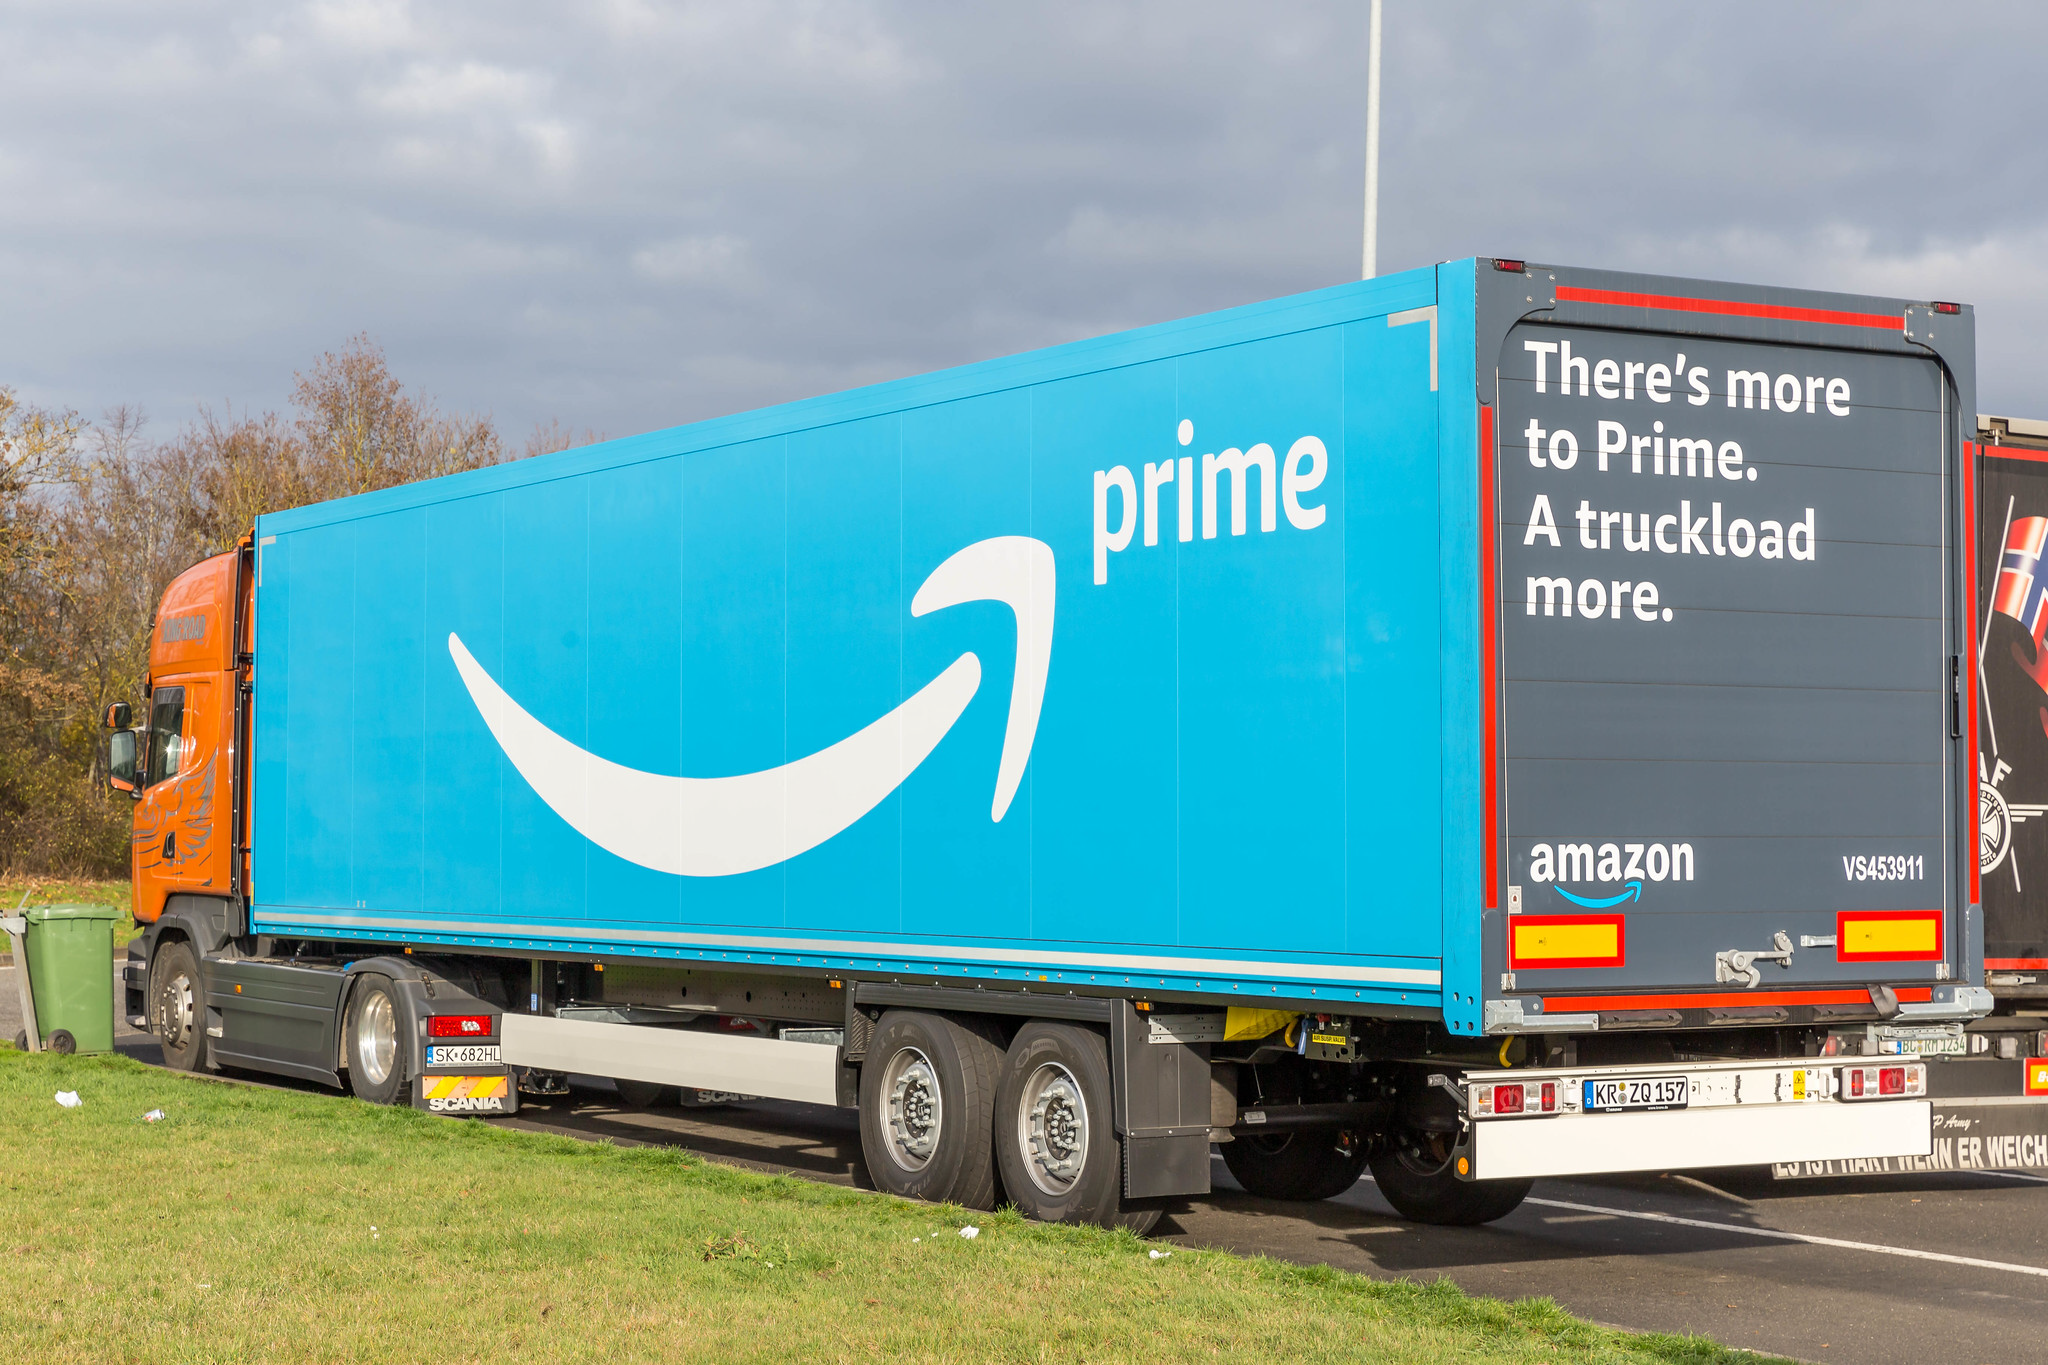
\includegraphics[width=\paperwidth]{images/cover-picture.png}}}
 \AtPageUpperLeft{\raisebox{-\bannerheight-\height}{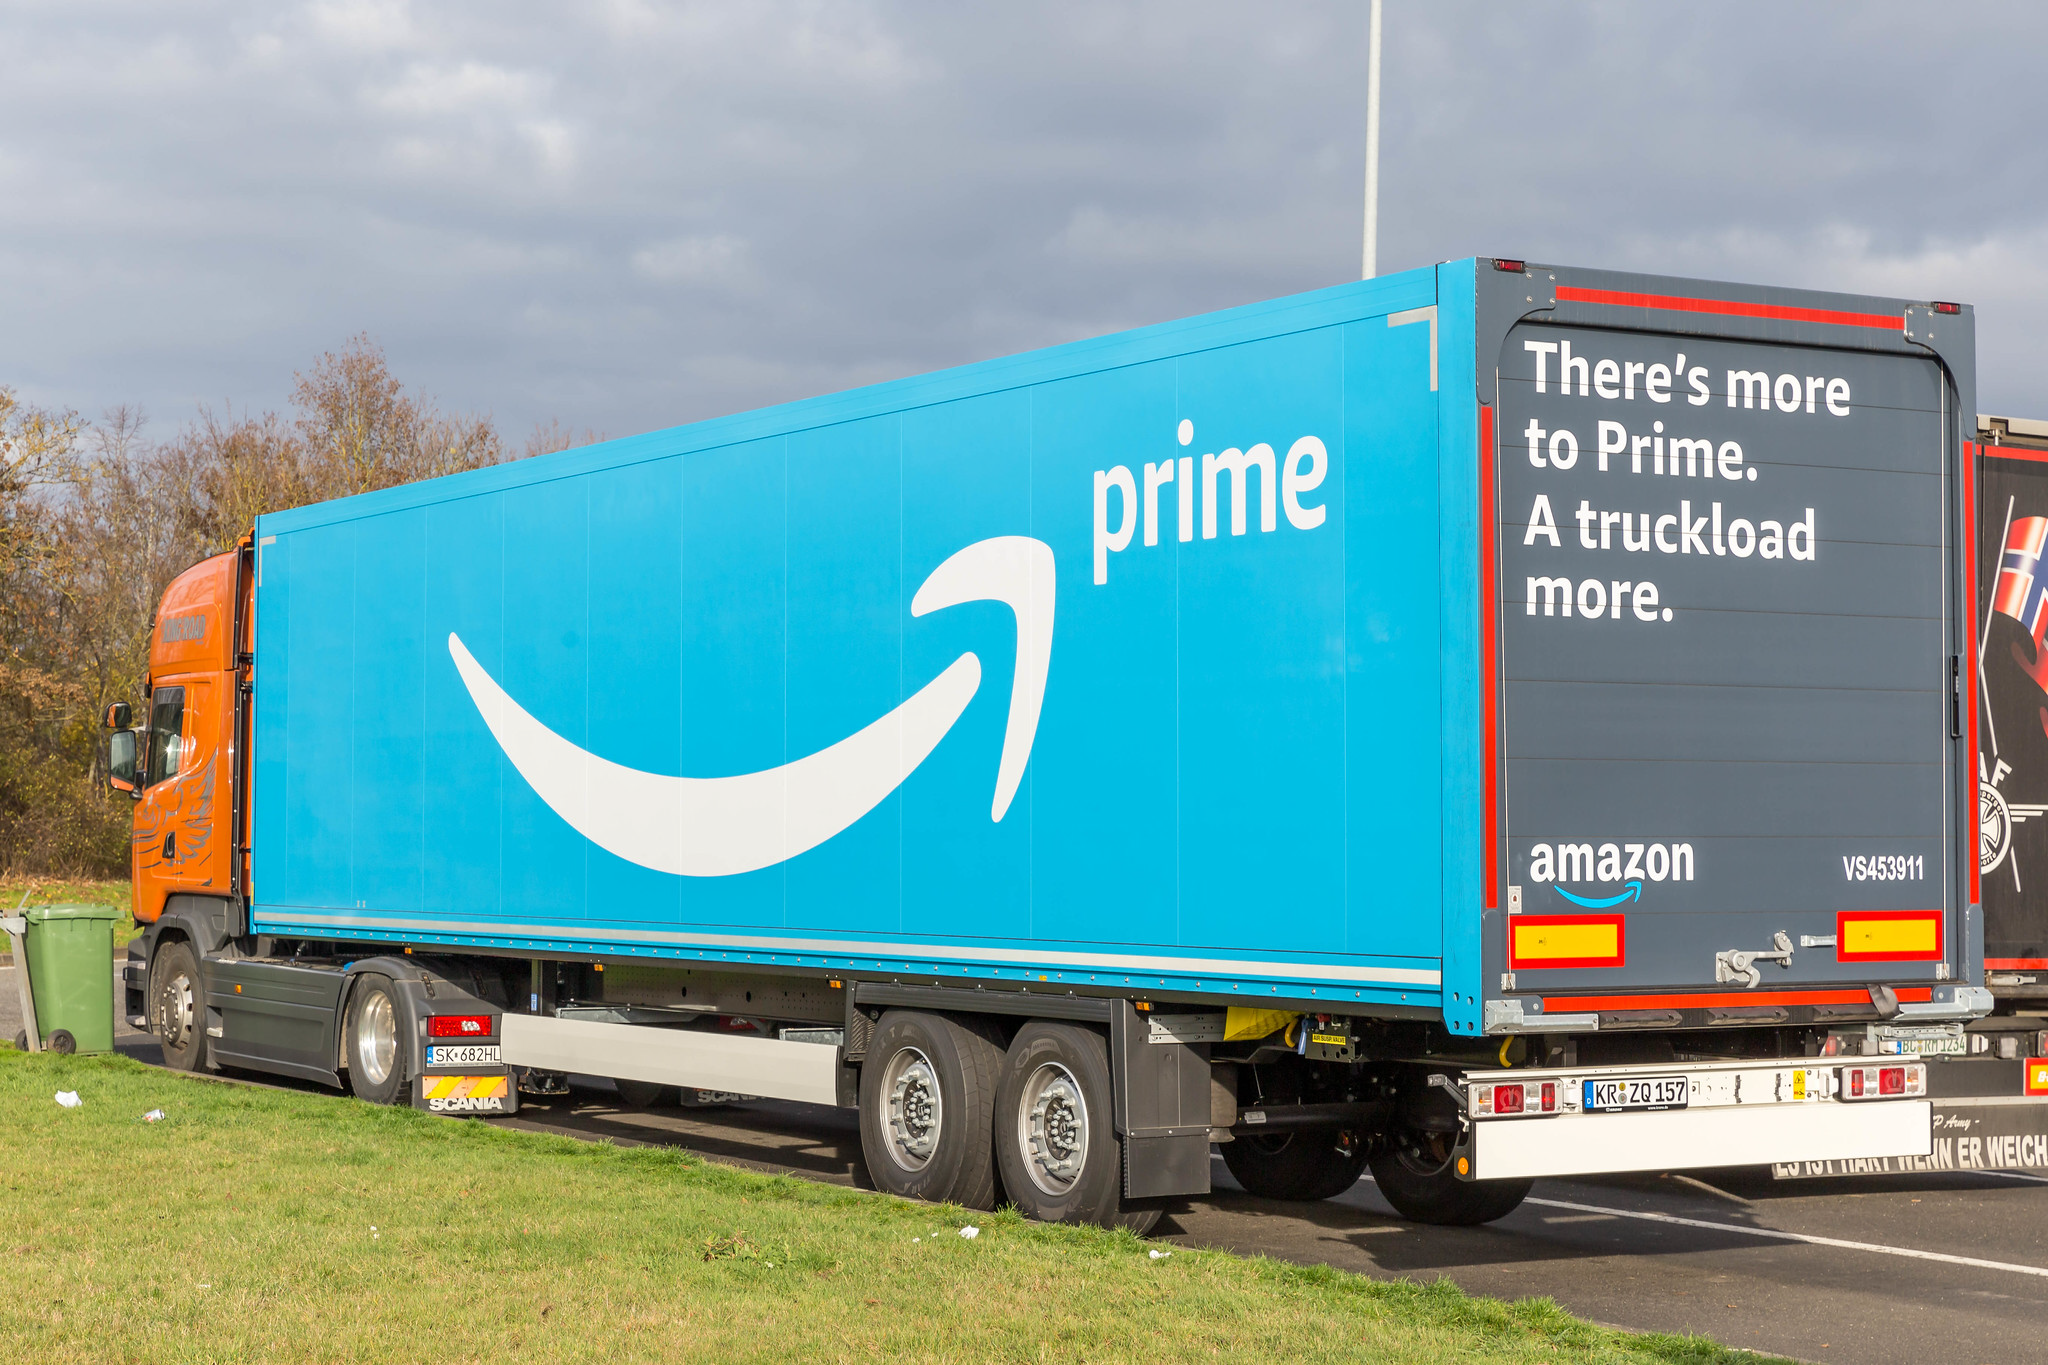
\includegraphics[width=\paperwidth]{images/cover-picture.png}}}
 }

% HERE GOES THE TITLE OF THE DOCUMENT
  \vspace{-5cm}{\relscale{1.75}{\textcolor{white}{Searching for
standards of fairness in the transportation justice literature}}}\par%
% HERE GOES THE DOCUMENT TYPE; CURRENTLY HARDCODED BUT COULD BE AN INPUT IN template.qmd
{\relscale{1.25}{\textcolor{Yellow}{Report (Draft)}}}\hfill
% HERE GOES THE DATE OF PUBLICATION
{\relscale{1.0}{\textcolor{LightGray}{2023-11-15}}}
        
% Report information: Needs information that is in file template.qmd
\begin{flushleft}
  \vspace{0.5cm} 
  % HERE GO THE AUTHORS AFFILIATIONS (ONLY NAME OF ORGANIZATION)
  % Needs to iterate by authors
      {\relscale{1.25}{\textcolor{Yellow}{Anastasia Soukhov}}} 
    % Needs to iterate by affilitations
          \hskip 10pt{\relscale{0.75}{\textcolor{LightGray}{McMaster
University}}} \par%
     
      {\relscale{1.25}{\textcolor{Yellow}{Ignacio Tiznado-Aitken}}} 
    % Needs to iterate by affilitations
          \hskip 10pt{\relscale{0.75}{\textcolor{LightGray}{University
of Toronto}}} \par%
     
      {\relscale{1.25}{\textcolor{Yellow}{Matthew Palm}}} 
    % Needs to iterate by affilitations
          \hskip 10pt{\relscale{0.75}{\textcolor{LightGray}{The
University of North Carolina at Chapel Hill}}} \par%
     
      {\relscale{1.25}{\textcolor{Yellow}{Steven Farber}}} 
    % Needs to iterate by affilitations
          \hskip 10pt{\relscale{0.75}{\textcolor{LightGray}{University
of Toronto}}} \par%
     
      {\relscale{1.25}{\textcolor{Yellow}{Antonio Páez}}} 
    % Needs to iterate by affilitations
          \hskip 10pt{\relscale{0.75}{\textcolor{LightGray}{McMaster
University}}} \par%
     
  \end{flushleft}

% Mobilizing Justice Logo
\AddToShipoutPictureBG*{\put(50,30)%
{
\includegraphics[width=0.5\textwidth]{images/mj-logo.png}%
}}

%-----------------------------------------------------------------------------%
% END OF TITLE PAGE
%-----------------------------------------------------------------------------%
\newpage

%-----------------------------------------------------------------------------%
% START OF HOW TO CITE PAGE
%-----------------------------------------------------------------------------%
\thispagestyle{empty}

\section*{Citing This Document}

This \href{https://example.com/summarizing-output}{report} is published under a Creative Commons \href{https://creativecommons.org/licenses/by/4.0/}{CC-BY Licence} 
\includegraphics[height=11pt]{images/cc-by.png}.

% HERE GOES THE TITLE OF THE DOCUMENT

  \vskip 20pt
  % APA style citation
  For attribution, please cite this work as:\\
  \vskip 1pt
  % This loop is for all authors but last! Check https://stackoverflow.com/questions/42354800/pandoc-template-different-separator-for-last-item
  % Also, it uses a custom function for extracting the first letter of the given name of authors (see partial header.tex). NOTE: IF THERE IS A MIDDLE NAME IT SADLY VANISHES
            {Soukhov, \ExtractFirstChar{Anastasia}.,}
          {Tiznado-Aitken, \ExtractFirstChar{Ignacio}.,}
          {Palm, \ExtractFirstChar{Matthew}.,}
          {Farber, \ExtractFirstChar{Steven}.,}
              {Páez, \ExtractFirstChar{Antonio}.}
          %  %  {Anastasia Soukhov},
    %  {Ignacio Tiznado-Aitken},
    %  {Matthew Palm},
    %  {Steven Farber},
    %  {Antonio Páez},
   (\the\year). \textit{Searching for standards of fairness in the
transportation justice
literature} (Report No. MJ-0001). Mobilizing Justice. \url{https://example.com/summarizing-output}
  \vskip 20pt
  %
  % Bibtex citation card
  %
  Or use this bibtex card:\\
  \vskip 1pt
  @report\{MJ-0001,\\
          % This loop is for all authors but last! Check https://stackoverflow.com/questions/42354800/pandoc-template-different-separator-for-last-item
           \hspace*{1.6cm} author = \{                                                                                  {Soukhov, Anastasia and} 
                                                                                  {Tiznado-Aitken, Ignacio and} 
                                                                                  {Palm, Matthew and} 
                                                                                  {Farber, Steven and} 
                                                                                                                          {Páez, Antonio}
                                                                                \},\\
           \hspace*{1.6cm} title = \{Searching for standards of fairness
in the transportation justice literature\},\\
           \hspace*{1.6cm} year = \{\the\year\},\\
           \hspace*{1.6cm} institution = \{Mobilizing Justice\},\\
           \hspace*{1.6cm} number = \{MJ-0001\},\\
           \hspace*{1.6cm} url = \{https://example.com/summarizing-output\}\\
  \}

\vspace*{\fill}
{\relscale{0.75}{\textbf{Image on the cover.} {Source: Marco Verch
(https://www.flickr.com/photos/160866001@N07/50597690137/)}.\\
\textbf{Image on the table of contents.} {Source: Progressive
Charlestown
(https://www.progressive-charlestown.com/2020/01/amazon-drivers-die-for-you.html)}.}}

%-----------------------------------------------------------------------------%
% END OF HOW TO CITE PAGE
%-----------------------------------------------------------------------------%
\newpage

%-----------------------------------------------------------------------------%
% START OF ABOUT PAGE
%-----------------------------------------------------------------------------%

\section*{About Mobilizing Justice}

The Mobilizing Justice Partnership is funded by the Social Sciences and Humanities Research Council (SSHRC). Based at the University of Toronto Scarborough, the national intersectoral research partnership aims to understand and address transportation poverty in Canada and to improve the well-being of Canadians at risk of transport poverty. Learn more at \url{www.mobilizingjustice.ca}.

% TABLE OF PARTNERS

\section*{Our Partners}
\begin{center}
\ctable[
%label = width,
width = \textwidth,
pos = ht,
left,
doinside = \relscale{0.87}{}
]{| >{\setlength{\baselineskip}{0.1\baselineskip}}>{\raggedright}X | >{\setlength{\baselineskip}{0.1\baselineskip}}>{\raggedright}X | >{\setlength{\baselineskip}{0.1\baselineskip}}>{\raggedright}X |}{}
{ \FL
Amalgamated Transit Union Canada                                                & Infrastructure Canada              & Transit App                                \LL
Autorité régionale de transport métropolitain (ARTM)                            & McGill University                  & TransLink                      \LL
Canadian Institute of Planners                                                  & McMaster University                & United   Way Greater Toronto   \LL
Canada Mortgage and Housing Corporation (CMHC)                                  & Memorial University                & University of British Columbia \LL
Canadian Urban Institute                                                        & Metrolinx                          & University of Manitoba         \LL
Canadian Urban Transit Association                                              & Ontario Ministry of Transportation & University of Oregon           \LL
The Centre for Active Transportation (TCAT), a project of Clean Air Partnership & Pantonium                          & University of Texas Austin     \LL
CIRODD (École de technologie supérieure)                                        & Pembina Institute                  & University of Toronto          \LL
CIRRELT (Université de Montréal)                                                & Region of Waterloo                 & University of Waterloo         \LL
City of Calgary                                                                 & RideShark                          & Urban Strategies               \LL
City of Edmonton                                                                & Simon Fraser University            & Via Transportation Inc.        \LL
City of Toronto                                                                 & Spare Labs                         & Ville de Montréal              \LL
City of Vancouver                                                               & SPIN                               & York Region                    \LL
Esri Canada                                                                     & Statistics Canada                  &    \LL
Federation of Canadian Municipalities	& Toronto Transit Commission (TTC)	& \LL
}
\end{center}

%-----------------------------------------------------------------------------%
% END OF ABOUT PAGE
%-----------------------------------------------------------------------------%
\newpage

%-----------------------------------------------------------------------------%
% START OF AUTHORS PAGE
%-----------------------------------------------------------------------------%

\section*{About the Author(s)}

  {\relscale{1.25}{\textcolor{Maroon}{Anastasia Soukhov}}}%
  % Needs to iterate by affilitations department
      \vskip 1pt{\relscale{0.75}{\textcolor{black}{School of Earth,
Environment and Society}}}%
   
  % Needs to iterate by affilitations name
      \vskip -8pt{\relscale{0.75}{\textcolor{black}{McMaster
University}}}%
   
  % Needs to iterate by email
      \vskip -8pt{\relscale{0.75}{\textcolor{black}{email: \url{soukhoa@mcmaster.ca}}}}%
   
  \vskip 15pt
  {\relscale{1.25}{\textcolor{Maroon}{Ignacio Tiznado-Aitken}}}%
  % Needs to iterate by affilitations department
      \vskip 1pt{\relscale{0.75}{\textcolor{black}{Department of
Geography and Planning}}}%
   
  % Needs to iterate by affilitations name
      \vskip -8pt{\relscale{0.75}{\textcolor{black}{University of
Toronto}}}%
   
  % Needs to iterate by email
      \vskip -8pt{\relscale{0.75}{\textcolor{black}{email: \url{i.tiznadoaitken@utoronto.ca}}}}%
   
  \vskip 15pt
  {\relscale{1.25}{\textcolor{Maroon}{Matthew Palm}}}%
  % Needs to iterate by affilitations department
      \vskip 1pt{\relscale{0.75}{\textcolor{black}{Department of City
and Regional Planning}}}%
   
  % Needs to iterate by affilitations name
      \vskip -8pt{\relscale{0.75}{\textcolor{black}{The University of
North Carolina at Chapel Hill}}}%
   
  % Needs to iterate by email
      \vskip -8pt{\relscale{0.75}{\textcolor{black}{email: \url{palmmatt@unc.edu}}}}%
   
  \vskip 15pt
  {\relscale{1.25}{\textcolor{Maroon}{Steven Farber}}}%
  % Needs to iterate by affilitations department
      \vskip 1pt{\relscale{0.75}{\textcolor{black}{Department of
Geography and Planning}}}%
   
  % Needs to iterate by affilitations name
      \vskip -8pt{\relscale{0.75}{\textcolor{black}{University of
Toronto}}}%
   
  % Needs to iterate by email
      \vskip -8pt{\relscale{0.75}{\textcolor{black}{email: \url{steven.farber@utoronto.ca}}}}%
   
  \vskip 15pt
  {\relscale{1.25}{\textcolor{Maroon}{Antonio Páez}}}%
  % Needs to iterate by affilitations department
      \vskip 1pt{\relscale{0.75}{\textcolor{black}{School of Earth,
Environment and Society}}}%
   
  % Needs to iterate by affilitations name
      \vskip -8pt{\relscale{0.75}{\textcolor{black}{McMaster
University}}}%
   
  % Needs to iterate by email
      \vskip -8pt{\relscale{0.75}{\textcolor{black}{email: \url{paezha@mcmaster.ca}}}}%
   
  \vskip 15pt

%-----------------------------------------------------------------------------%
% END OF AUTHORS PAGE
%-----------------------------------------------------------------------------%
\newpage

%-----------------------------------------------------------------------------%
% START OF ACKNOWLEDGMENTS PAGE
%-----------------------------------------------------------------------------%

\section*{Acknowledgements}

  This report would not have been possible without the help and
  inspiration of many individuals not listed as authors. In the early
  stages of this report we received invaluable help from specialists at
  the University of Toronto as we learned about various approaches to
  literature reviews, particularly the Research Services and Liaison
  Librarians. These experts provided guidance in cornering down the
  topic, identifying guidance material on literature synthesis and
  relevant databases, and eased us into the world of knowledge
  synthesis. Though our path diverged from a traditional scoping review,
  the protocol published on September 2022 (found
  \href{https://osf.io/rsb92}{here}) was followed with only minor
  changes, with only a reduction in the databases searched due to
  resource constraints. We also wish to acknowledge the many hours of
  work by undergraduate and graduate research assistants who poured
  through title and abstract screening to help determine full-text
  eligibility at the earliest stages of our search. The volume of
  literature initially reviewed was greater than any of us had
  experienced before, but important to be as inclusive as possible. For
  this support, we are deeply thankful to Jan Domalaon, Dancel Gayle,
  Eryn Maloney, Mahdis Moghadasi, Anika Munir, and Subaita Refaaf. The
  views and opinions expressed here, as well as any equivocations and/or
  awkwardness are the authors' and the authors' alone.

%-----------------------------------------------------------------------------%
% END OF ACKNOWLEDGMENTS PAGE
%-----------------------------------------------------------------------------%
\newpage

%-----------------------------------------------------------------------------%
% START OF TABLE OF CONTENTS PAGE
%-----------------------------------------------------------------------------%

% Change the geometry of this one page so that the table of contents begins below the banner image instead of on top of it

\settoheight{\bannerheight}{%
  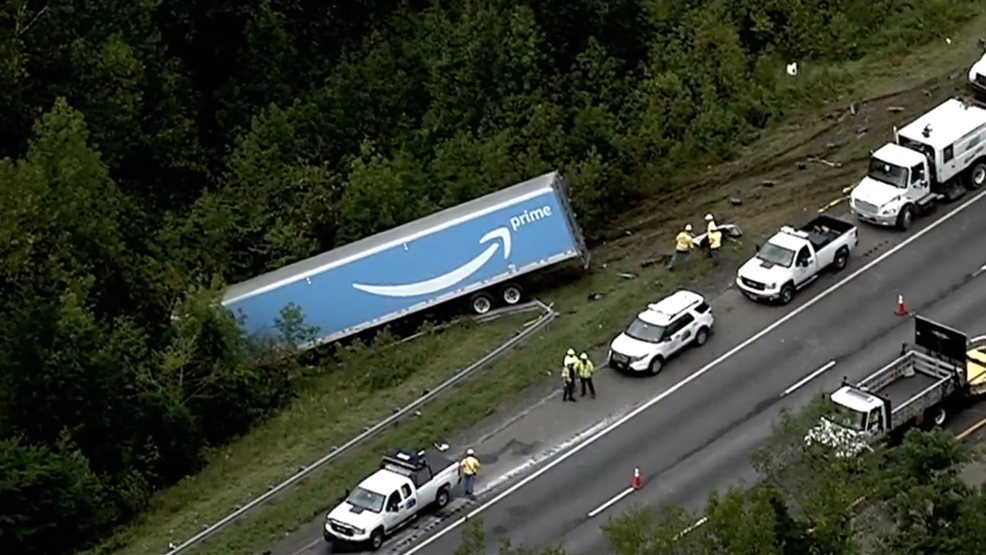
\includegraphics[width=\paperwidth]{images/toc-picture.png}%
}

\newgeometry{left=1.9cm, right=1.9cm, top=\bannerheight, bottom=1.9cm}


% Table of contents picture top
\AddToShipoutPictureBG*{%
 \AtPageUpperLeft{\raisebox{-\height}{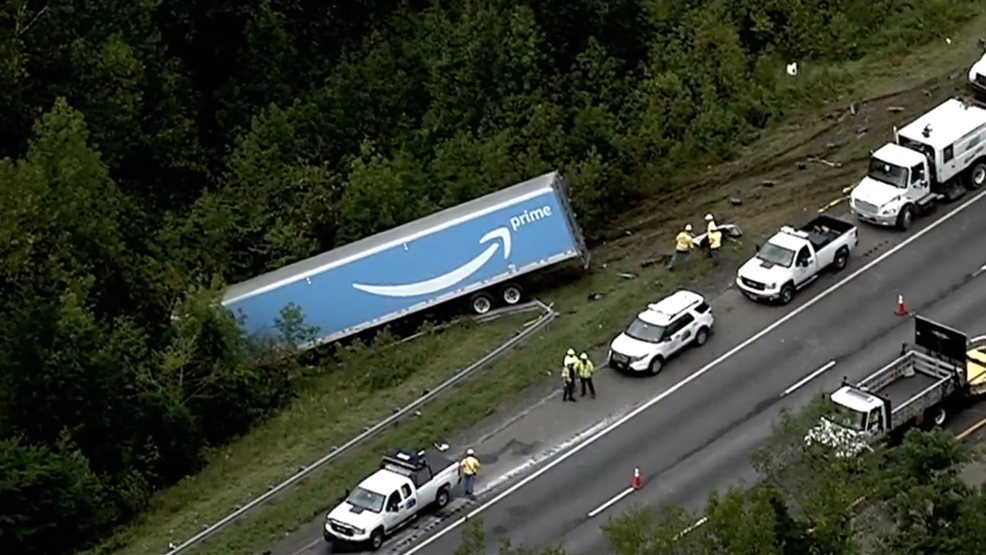
\includegraphics[width=\paperwidth]{images/toc-picture.png}}}}

% Title for the table of contents
\setcounter{tocdepth}{1}
\tableofcontents
\restoregeometry

%-----------------------------------------------------------------------------%
% END OF TABLE OF CONTENTS
%-----------------------------------------------------------------------------%
\newpage\ifdefined\Shaded\renewenvironment{Shaded}{\begin{tcolorbox}[enhanced, interior hidden, borderline west={3pt}{0pt}{shadecolor}, breakable, sharp corners, frame hidden, boxrule=0pt]}{\end{tcolorbox}}\fi

\hypertarget{executive-summary}{%
\section{Executive Summary}\label{executive-summary}}

Modern societies provide people with varying degrees of mobility and
accessibility, from low wage Amazon workers' depending on infrequent bus
service, to Jeff Bezos taking private flights into space. Societies
implicitly tolerate different levels of inequality in access, though
these levels are occasionally made legible through policy standards. For
example, U.S. transit agencies are required to set and adhere to maximum
levels of disparity in service quality between minority and non-minority
routes as defined by the U.S. Civil Rights Act. In contrast to prior
reviews on how to measure inequality in transportation systems, this
report is concerned with the implied or explicit standards that are used
to judge whether the measured inequalities are fundamentally ``fair'' or
unacceptable. The present study achieves this objective by scanning the
state of academic knowledge in defining ``fairness'' in the transport
domain.

Borrowing from philosophers of justice (Jaggar 2009), the report's
authors ask the following questions about existing standards of fairness
in practice:

\begin{itemize}
\tightlist
\item
  \textbf{Where and when} are equity standards applied within the
  research depending on location and time of publication? How are
  context-specific planning processes changing?\\
\item
  \textbf{Who} benefits and is burdened by transportation systems? Along
  which lines of identity are transportation inequities examined?\\
\item
  \textbf{What} are those benefits and burdens of transportation
  systems? Are they qualified in sidewalk widths, bus frequency, travel
  times, accessibility, or some other consideration?\\
\item
  \textbf{How}: are equity standards and inequities measured? Are they
  infrastructure provision thresholds, acceptable pollution levels, or
  some other kind of cut off? How are these studies born out of broader
  notions of justice, i.e.~disability rights, environmental justice,
  egalitarianism, or something else?
\end{itemize}

\textbf{Methods}

The authors conducted a scoping review of the literature. The review
involves entering combinations of equity-related keywords into academic
databases to identify relevant studies. The team initially discovered
6,832 references from three diverse databases that they shrunk to a
final corpus of studies using a four-step process:

\begin{enumerate}
\def\labelenumi{\arabic{enumi}.}
\tightlist
\item
  A total of 611 duplicate studies were removed.\\
\item
  The researchers, supported by a team of trained research assistants,
  reviewed the remaining titles and abstracts for relevance, with 4,511
  studies excluded for not sufficiently addressing transportation
  equity.\\
\item
  The full-texts of the remaining 1,711 studies were reviewed. At least
  two trained research assistants reviewed each document, with one of
  the the main researchers (listed as authors) breaking any ties. This
  resulted in 1,545 additional studies being excluded. At this stage,
  studies could be excluded if they did not include any standard for, or
  conceptual grounding for, equity.\\
\item
  The researchers examined the final corpus of 165 studies to extract
  data on the ``When'', ``Where'', ``Who'', ``What'', and ``How'' of
  transport equity in each study. This included annotating the methods
  used, standards suggested, and inferring conceptualizations of equity
  that may connect to broader notions of justice.
\end{enumerate}

\textbf{Results}

\textbf{When and Where: the contexts of justice}. Most (60\%) studies
that deployed standards for equity stem from the Global North, including
cases from Europe, the U.S., Canada, Australia, New Zealand, Japan, and
Israel. The focus of these studies is on groups seen as disadvantaged
within their respective national contexts, and strive to relate
standards to national policies or issues. In contrast, research stemming
from the Global South tends to adopt international standards in
analyses, such as the U.N.'s Sustainable Development Goals (SDGs).
Within the Global South, studies most commonly cover Asia, followed by
Latin America. Studies in the latter region focus disproportionately on
mobility barriers and the financial affordability of transportation.
Studies pertaining to Africa are numbered, though they cover a broader
scope of issues including informal transportation, citizens'
accessibility needs, and infrastructure development needs. Across the
globe, the studies reviewed apply equity standards overwhelmingly to
urban contexts (85\%) and are concerned with a focused set of issues
around the need for and the impacts of daily mobility. Studies on rural
contexts are broader in the topics examined, from the equity of ferry
service in the Philippines to the impacts of road construction on remote
Amazonian communities.

\textbf{Who: the subjects of justice.} Income groups are studied most,
followed by age groups, and people with disabilities. People with low
incomes generally experience the least benefits and greatest burdens of
transportation systems, including regarding costs and pollution
exposure. Studies examining equity with respect to age demonstrate how
older adults and children face different levels of access to key
destinations due to differences in their capabilities. Many studies
apply universal design guidelines and laws as equity standards to
evaluate the equity of transportation systems for people with
disabilities. Finally, researchers also frequently develop composite
indices of vulnerability to identify neighbourhoods with high
concentrations of multiple vulnerable populations. This approach is
common when examining environmental justice impacts.

\textbf{What: the tools of mobility.} Most studies that deploy equity
standards apply them to either transit (37\%) or pedestrian modes
(25\%). Many transit analyses are multimodal in nature, comparing
accessibility by transit to accessibility by automobiles as an implicit
standard. Others combine transit with non-auto modes to examine access
for households without vehicles. These studies focus on delivering
equitable mobility, sometimes in context of also meeting climate goals.
However, they often fail to include explicit minima of service that
should be provided to different populations. In contrast, rights-based,
infrastructure-focused studies apply principles of universal design in
the study of transport systems and related infrastructure.

\textbf{What: the benefits of mobility.} Studies measure either movement
(i.e., trips taken, trip quality, etc.) or the potential for movement
(i.e.~accessibility to specific destinations, or generally), with most
studies focused on the latter. Over a quarter of the papers that focus
on accessibility do not consider specific destinations, but instead
concentrate on the accessibility of the trip (i.e., level of service,
barriers of infrastructure) or bundles of destinations. Other studies
are centred on particular destinations considered as essential,
including employment, healthcare, grocery stores, and greenspace. Access
to community support or places of worship, as well as childcare
activities are far less common in the literature reviewed.

\textbf{How: concepts and standards of justice.} The most common
standards found in the literature, which we term opportunity standards,
are defined using cut offs in access to opportunities (37.2\%). Almost
as common is the formulation of standards that use thresholds related to
the perceptions or activities of specific populations (35.8\%); we call
these population standards. The latter often includes standards informed
by public health, such as the number of physical activities undertaken
in a week and perceived life satisfaction. Opportunity standards are
evaluated through horizontal equity and spatial equity lenses, while
population ones are evaluated through well-being frameworks. Another
category of standards that emerged from the literature are based on
infrastructure, and these include adherence to universal design
guidelines or specific benchmarks for road network characteristics.
Standards of thsi kind are comparatively less common in the literature
and are often framed in terms of rights, particularly as they relate to
achieving universal design. Infrastructure standards around sustainable
infrastructure (i.e.~block lengths or distance between transit stops)
are also evaluated through vertical, horizontal and spatial lenses. The
distribution of studies with respect to the kinds of standards deployed,
and the broader concepts of justice used, are presented in the Figure
below:

\begin{figure}

{\centering 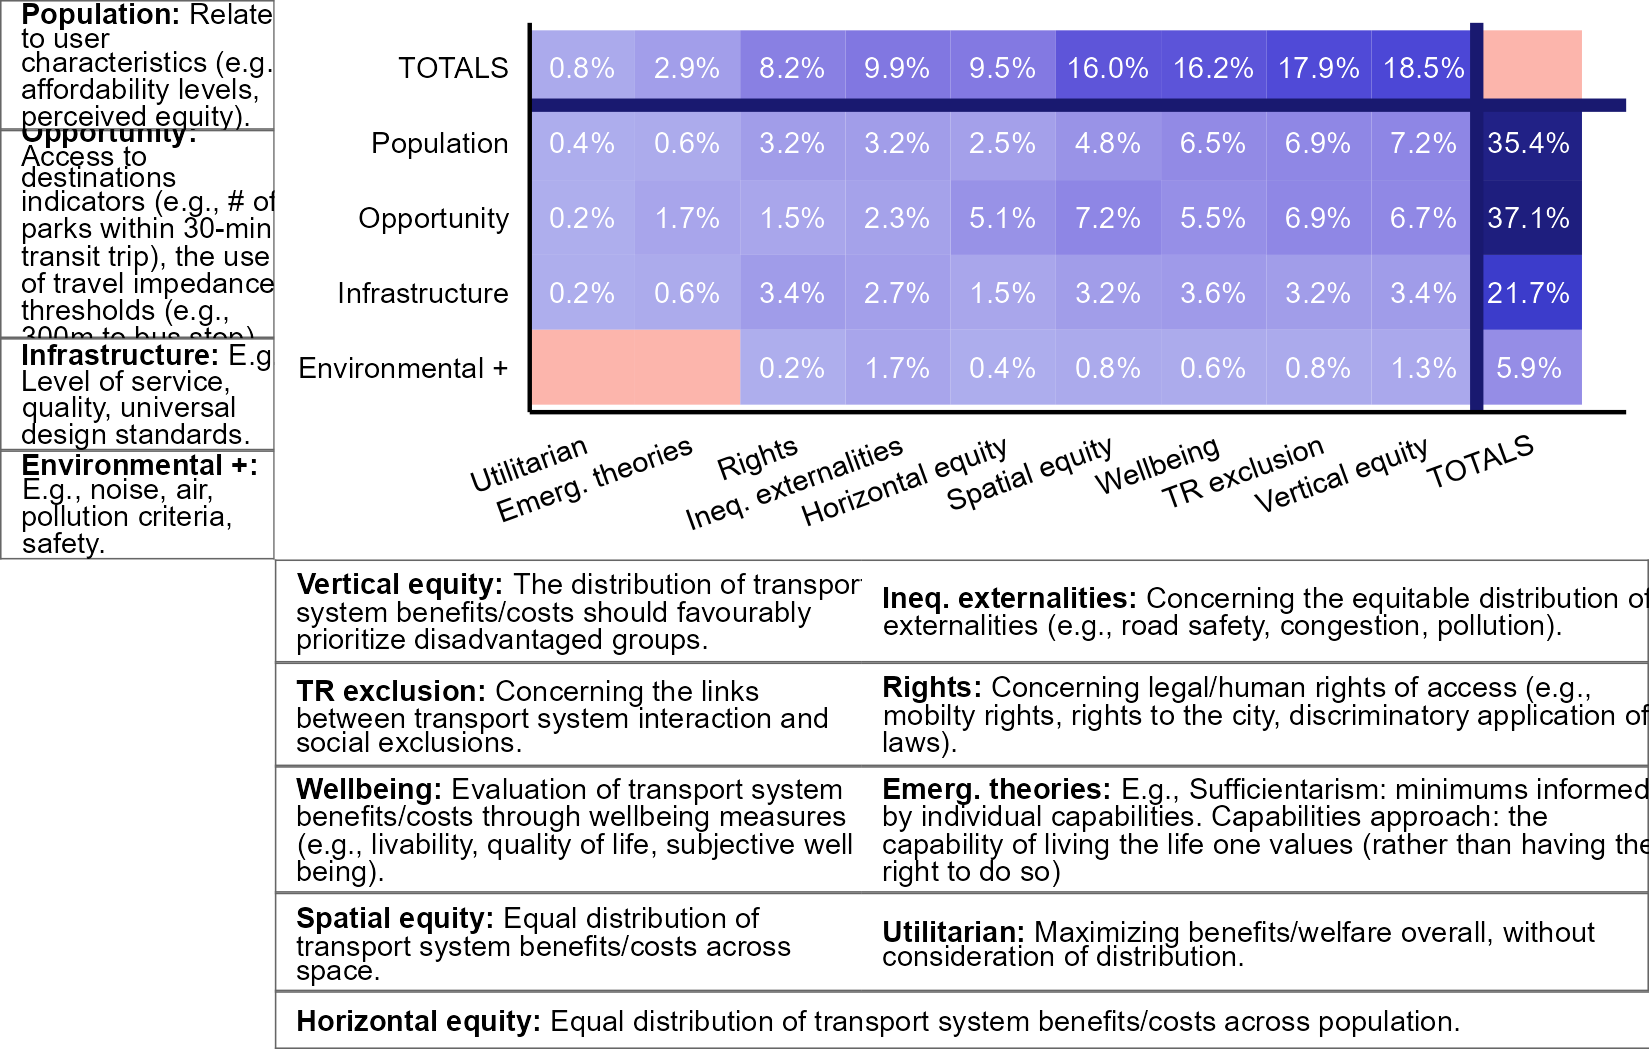
\includegraphics{figures/standards_conc_percentages_plot_and_table.png}

}

\caption{The proportion of equity standards (vertical axis) within each
type of equity conceptualization (horizontal axis) category.}

\end{figure}

\textbf{Calls to Action}

The review conducted for this report provides a snapshot of the state of
knowledge today in terms of how standards of fairness are developed and
deployed. The review is telling both in terms of what it reveals about
the literature, what is covered and what is not. Based on these, the
authors challenge practitioners, researchers, advocates, and governments
to commit to five calls to action:

Call 1: Underpin standards in rigorous concepts of justice.

The standards of equity used in research are often weakly linked to any
legally, intellectually, or publicly accepted concepts of justice. Many
standards are arbitrary. For example, the 15-minute city sets a
threshold that is easy to remember, but is this really what is needed to
achieve sufficient sustainable mobility for urban residents, as opposed
to a 10 or 20 minute city? And what conceptualization of human need
should determine what services are essential enough to be included
within this threshold, and for whom?

Call 2: Develop creative methods for systems-thinking approaches to
equity.

Mixed-methods research can help governments set meaningful standards by
better linking quantitative thresholds with qualitative assessments of
well-being, as well as freedom of movement and perceived access, among
other facets of transportation. Yet most of the research reviewed is
purely quantitative or, to a much lesser degree, purely qualitative. The
constant deployment of metrics Lorenz Curves of Gini coefficients
without research on where such measures need to be to improve quality of
life (i.e., a standard), will not help governments with limited
resources achieve the best possible equity outcomes within their
respective contexts. Mobilizing Justice's Priority Populations working
group was inaugurated to advance new research in this area.

Call 3: Making data available is a matter of justice.

Several areas of critical importance, such as access to care and
community, are under-researched, and the authors suspect this relates to
lack of data on these kinds of destinations. Furthermore, data issues
prevent the application of many methods of equity analyses in the Global
South. The production, availability, transparency, and ownership of data
is a matter of justice on which governments and NGOs should act. In the
Canadian context, Mobilizing Justice's National Survey working group is
working to advance data practices by conducting the first national
survey on transportation poverty and striving to make data available in
the form of Open Data Products.

Call 4: Develop more direct and explicit links between standards and
lived experiences.

Linking standards to lived experiences and individual outcomes can help
increase the likelihood of their adoption by governments. Further, they
can help decision makers understand the role of transportation in
improving policy outcomes in other domains like nutrition, physical and
mental health, education, and human development. These links can help
make the standards used in research and policy more comprehensible and
relatable to community members and people with lived experience
navigating unequal mobility systems. Mobilizing Justice launched it's
Data Driven Standards working group to advance research in this area.

Call 5: Rigorously evaluate interventions and policies.

Approximately 10\% of the studies reviewed aimed to assess
interventions. Delivering new equity-focused policies and programs that
do not actually advance equity harms communities, metastasizes mistrust,
and delegitimates future efforts to promote transportation justice.
Furthermore, policies that benefit one group of people in one context
may not benefit other groups in other situations. A deep breadth of
equity evaluations is needed to avoid failure and guide policymakers
towards interventions that will work for the communities they serve.
Mobilizing Justice launched its Innovative Pilots working group to begin
filling this gap, through further work is needed.

\newpage

\hypertarget{reading-guide}{%
\section{Reading guide}\label{reading-guide}}

This is your guide to scanning this document.

If you are primarily interested in the motivation behind this report,
read the first section, \protect\hyperlink{sect1}{Just transportation?}

Keen to jump straight to a description of the conceptual framework for
transport justice? See the second section, particularly the subsection:
\protect\hyperlink{sect2.2}{A framework to analyze questions of
justice}.

Interested in the methodological details of the literature review? See
\protect\hyperlink{sect3}{section three} and extended information in the
\protect\hyperlink{sect8}{Appendix}

Care more about the results and the critical appraisal of the results
from the review? See sections \protect\hyperlink{sect4}{four} and
\protect\hyperlink{sect5}{five}, respectively.

Want to know about our calls for action to move transport equity
analysis and standard-setting substantively towards questions of
transport justice? Read the sixth section
\protect\hyperlink{sect6}{Moving forward: calls for action} and the
final concluding section \protect\hyperlink{sect7}{Final remarks}. These
sections are geared to both researchers and decision-makers.

\newpage

\hypertarget{glossary}{%
\section{Glossary}\label{glossary}}

\begin{itemize}
\tightlist
\item
  \textbf{Accessibility}: the potential to reach destinations.
\end{itemize}

\begin{itemize}
\item
  \textbf{Equality}: a state where every group is treated identically.
\item
  \textbf{Equity}: the distribution of benefits and burdens of things
  among the population, with a particular emphasis on those with the
  least advantage and quality in their outcomes.
\item
  \textbf{Equity standards}: tools for answering the question of how to
  distribute the burdens and benefits and to whom? When operationalized
  standards effectively define what is fair.
\item
  \textbf{Fairness}: a state of being that is achieved when a collective
  and individuals are treated equally and without bias as defined by
  their morals and values.
\item
  \textbf{Justice}: A political ideal whereby people give and receive
  what they are due.
\item
  \textbf{The temporal-spatial context of justice}: the answers to
  ``Where?'' and ``When?''. What regions, within what countries, spatial
  contexts, point of time, and processes of planning are impacting
  transport systems?
\item
  \textbf{The subjects of justice}: the answer to ``Who?'' is the focus
  of justice.
\item
  \textbf{The objects of justice}: the answer to ``What?'' is the focus
  of justice; what are the things that characterise (in)justice.
\item
  \textbf{The methods for justice determination}: the answer to ``How?''
  is justice defined and markers towards it tracked.
\item
  \textbf{The rationale to justice}: the ``Why?''. The rationale
  connects with the context, subject, object and methods used for
  justice determination.
\item
  \textbf{Mobility}: The potential to move.
\item
  \textbf{Policy}: A deliberate system of principles to guide decisions
  and achieve desired outcomes.
\end{itemize}

\begin{itemize}
\tightlist
\item
  \textbf{Space-time convergence}: the main product of a transportation
  system is to reduce the time needed to cover a unit of distance; this
  effect makes space and time converge.
\end{itemize}

\newpage

\hypertarget{sect1}{%
\section{Just transportation?}\label{sect1}}

\begin{quote}
``\emph{To be wealthy and honored in an unjust society is a
disgrace.}''\\
--- Confucius, The Annalects
\end{quote}

The fiery wake of a rocket could be seen ascending, piercing the sky
above West Texas. It was the morning of July 20, 2021, and on board of
the rocket was a small group of four passengers that included Jeff
Bezos, the founder of Amazon and then the world's richest person
(Harwood 2021). The mission that day was among the first-ever private
suborbital passenger flights, and the adventure (described as
``intense'' by one of the passengers) lasted a total of 10 minutes and
10 seconds (Harwood 2021). In addition to intense, the undertaking was
expensive: a seat for the flight had previously been auctioned for no
less than \$28 million USD (Griffin 2021). Before it was even 10:00 am
(EDT), Bezos was back from his excursion, and he took time to declare
that this was the ``{[}b{]}est day ever''. To reporters covering the
event he said ``I want to thank every Amazon employee and every Amazon
customer, because you guys paid for all of this'' (Johnson and Anilkumar
2021).

Meanwhile, firmly grounded on planet Earth, the employees whom Bezos
thanked for his suborbital jaunt were struggling with some very mundane
problems of their own, and none as lofty as conflicting schedules that
prevented them from flying in rockets (Griffin 2021). According to
reports, people employed directly or indirectly by Amazon for warehouse
or delivery work had, for years, been treated to ``inhumane'' conditions
(Fung 2018; Scott 2019; Greene 2021), and subjected to surveillance on
the job, degrading schedules that drove drivers to urinate in bottles,
crushing demands for productivity quotas that led to injury, all the
while facing little or no job security. From this perspective, they were
treated less with gratitude and more as disposable inputs to feed
Amazon's earnings and consumers' demands (Tung and Berkowitz 2020; BBC
2021; Reese and Alimahomed-Wilson 2022; Middleton 2023).

Coverage of the July 20 launch by the mainstream media was in many cases
uncritical. ``We're going to build a road to space so that our kids and
their kids can build a future'' Bezos declared, before adding
``\ldots we need to do that to solve the problems here on Earth''
(Johnson and Anilkumar 2021). Few reporters saw it fit to ask what
problems the billionaire planned to solve on Earth, or what kind of
future Bezos was trying to build, and for whose children. In other
words, the billionaire was not confronted with questions about what his
trip did \emph{for whom} and \emph{to whom}. A less dispassionate
observer might have been excused for wondering (possibly aloud) about
the basic \emph{fairness} of a man amassing a nigh unimaginable fortune
that allowed him to build and fly his own spaceship, while masses of his
employees were treated as throwaway cogs in the vast apparatus of his
emporium\footnote{Not unlike in the empire of another space billionaire,
  where things feel like the future except for the lives of workers
  (Wong 2017), and everything soars---including worker injuries (Taylor
  2023).}.

The question of \emph{fairness} is not a simple one. Most of us would
probably have been stumped to explain in a precise way just why the
above picture was disturbing. \emph{Justice} is a political ideal based
on the principle that individuals should be treated in a \emph{fair} and
\emph{equitable} manner (Gössling 2016, 2), giving and receiving
whatever they are \emph{due} (Jaggar 2009, 1--2). The political (and
contested; Vanoutrive and Cooper (2019)) nature of the concept presents
challenges that are only narrowly amenable to scientific inquiry. For
starters, the notion that people are ``due'' something depends on the
values of a society, as embodied in its systems and institutions (Karner
et al. 2020a). Values, in turn, are not subject to natural laws, but
rather are the result of intersubjective realities, which is to say
illusions whose legitimacy derives from a collective will to believe.
For example, justice would likely mean something very different to a
person in a democratic society, than to another in a society where they
owed their all to some collective illusion (e.g., the state, or a
monarch). As well, the meaning of ``justice'' would likely differ in yet
another society where very few owned most, and most owned very little
due to a different illusion (e.g., that wealth equates merit). In these
two hypothetical cases, elucidating the meaning of ``fair'' would in all
certainty be beyond the dreams of most, since fair would be whatever
organizational structures with power (e.g., the state, the monarch, or
the extremely wealthy) said it was. In contrast, in democratic
societies\footnote{Paraphrasing, democracy is the worst of collective
  illusions, except for all others.} individual rights tempered by a
collective vision are valued above the whims of the few. In such a
setting, the task of defining a ``just'' distribution of the burdens and
benefits of things---from income, to roads, to space travel---quickly
becomes muddled, encumbered even, by the necessity to pay attention to a
multitude of voices, not all of them equally loud.

The rocket that took Bezos to the edge of space is a somewhat rare
example of a transportation technology, a tool of space-time
convergence. By enabling movement at very high speeds, rockets
might---one day, at some indeterminate point in the future---prove
essential to the expansion of the human species beyond our home planet.
But in the present moment, the benefits of a private suborbital flight
(e.g., the joy of movement, the sense of adventure, the awe of seeing
Earth from space) are for a few, whereas the burdens (e.g., the use of
non-renewable resources, the climate-altering emissions) affect us all,
and not evenly at that. The benefits of public transportation, a much
more common transportation technology, are for most, but in many cases
we have penny-pinched these systems, leaving them moribund, while
concentrating the costs on those who have less (Jeff Allen and Farber
2020; Kaeoruean et al. 2020). In a plutocratic society, those with most
can (and often do argue\footnote{Either directly, as in the so-called
  Techno-optimist Manifesto (Andreessen 2023), or through their
  mouthpieces (McArdle 2021)}) that this distribution of burdens and
benefits is fair since both benefits and burdens are earned. The fact
that the likes of Bezos do travel to space is proof that the likes of
Bezos are due those trips. In a democratic society, the members of the
collective might actually agree that large rewards (e.g., space flight)
must be offered to highly qualified individuals (e.g., Bezos) to entice
them to take important responsibilities (e.g., founding and leading
Amazon). The fact that some must give up jobs because it is too time
consuming to reach them by public transportation would constitute proof
that those people should have studied more, been earlier risers, worked
harder (Spurr 2015; Greisman 2017). Again, the members of the collective
might believe that this is a fine state of affairs, having come to this
conclusion of their own accord or after being persuaded by billionaires.
Or, contrariwise, the members of the collective might decide that this
state of affairs is \emph{unjust}: the \emph{values} of those in charge
of defining what is ``fair'' matter.

Multiple national and cross-national studies suggest that people in many
societies do indeed have some tolerance for inequality (Kiatpongsan and
Norton 2014): it would appear that \emph{some} stratification, as
suggested by Davis and Moore (1945), is perceived as fulfilling a
valuable function. However, extreme inequality is often frowned upon,
and can lead to social dysfunction and other ills (Acemoglu and Robinson
2000; Taydas and Peksen 2012; Du, King, and Chi 2019; Houle et al.
2022). But the perceptions of what is ``fair'' are neither universal or
static. Instead, they are malleable, and can be affected by the
existence of opportunities for social mobility (Shariff, Wiwad, and
Aknin 2016; Artige, Lubart, and Neuss 2019), by exposure to inequality
(Schröder 2017; García-Castro et al. 2023), by learned helplessness (Y.
Kim, Jung, and Na 2022), and even by how information about inequality is
communicated to the public (Walker, Tepper, and Gilovich 2021). It
follows that, in general terms, there are at least three different
manners of thinking about inequality\footnote{Karel Martens (2016), in
  the introduction of his landmark text, talks about explanatory and
  prescriptive theories of justice; despite the saying ``the arc of
  history is long and bends toward justice'', it is unlikely that a
  predictive theory of justice exists.}: 1) in a \emph{positive} (or
descriptive) manner, as the current or historic state of the
distribution of benefits and burdens of things; 2) also descriptively,
as the \emph{perceptions} about the distribution of those benefits and
burdens; and 3) normatively (or prescriptively), as the desired or ideal
state of the same. Clearly, the three may coincide (e.g, if the
perceived levels of inequality matched actual inequality and also how
much of it the public desired). However, they do not necessarily have
to, and in many cases will differ from one another. Measuring inequality
as it is and in the most objective way possible, is an essential task to
decide whether there is a need to develop inequality-related policies to
increase fairness. In turn, measuring the perceptions of inequality, in
the most accurate way possible, may be important to achieve sufficient
public buy-in in order to enhance the chances that given policies will
succeed.

Transportation systems, as a class of essential technologies that
facilitate or impede social inclusion and activity participation
(Church, Frost, and Sullivan 2000; Lucas, Grosvenor, and Simpson 2001;
Social Exclusion Unit 2003; Cass, Shove, and Urry 2005; Casas 2007;
Preston and Raje, n.d.; Páez et al. 2009), have increasingly come into
focus from the perspective of equity. In response to this focus, a
lively and rapidly growing literature has emerged on the topic (see
\emph{inter alia} (Karel Martens 2016; Di Ciommo and Shiftan 2017; Guo
et al. 2020; Karner et al. 2020a; Vecchio, Tiznado-Aitken, and Hurtubia
2020; R. H. M. Pereira and Karner 2021; Wee and Mouter 2021; Zhang and
Zhao 2021; E. Desjardins, Higgins, and Paez 2022; Karner, Pereira, and
Farber 2023)). A cynical rationale for this interest could be that
keeping track of objective and perceived inequalities can serve \emph{at
the very least} as a gauge of social discontent (as Chilean authorities
discovered to their woe when an increase in Santiago Metro's fares
became a flashpoint for social inequalities, and sparked a period of
massive demonstrations and unrest in October 2019; (BBC News, Latin
America 2019; Díaz Pabón and Palacio Ludeña 2021)). More optimistically,
in democratic systems, tracking objective and perceived inequalities
could be of interest for governing bodies to respond to popular demands
for fairness. Several challenges arise when approaching this endeavor.
The notorious complexity of transportation systems is one of them:
transport systems simultaneously move people, goods, and information.
Emerging technologies and service models can swiftly change the balance
of benefits and burdens among a population (Guo et al. 2020), turning
both users and service providers into digital rentiers (Birch and
Cochrane 2022). The benefits and burdens of transportation systems are
diffuse over space and time. For example, transportation systems
engineered to offer higher mobility for people \emph{somewhere}, can
simultaneously cut others off from essential opportunities
\emph{elsewhere}, as Raje (2004) poignantly illustrated with examples of
infrastructure in the UK. Furthermore, the shades of policies past can
continue to haunt a region and even the planet for decades or longer, as
shown by the legacy of displacement and decay caused by urban highways
all across the US (Archer 2020) and the time horizon for the impacts of
climate change to be fully felt (Markolf et al. 2019).

But complexity is no excuse to shirk the task.

The objective of this report is to scan the state of knowledge in terms
of defining and operationalizing ``fairness'' in the transportation
domain. Much research has been devoted to the issues of \emph{measuring}
equity in transportation, including (among many others) Ramjerdi (2006),
A. Delbosc and Currie (2011a), T. F. Welch and Mishra (2013), Karel
Martens, Bastiaanssen, and Lucas (2019), and Pritchard, Zanchetta, and
Martens (2022). Further, there are multiple sources that discuss the
conceptual and philosophical foundations of equity and fairness in
transportation (e.g., Karel Martens 2016; R. H. M. Pereira, Schwanen,
and Banister 2017; Vanoutrive and Cooper 2019). Finally, previous
reviews of planning documents have investigated equity from narrowly
scoped perspectives, such as accessibility (Boisjoly and El-Geneidy
2017) or a particular mode of transportation {[}e.g., cycling; Doran,
El-Geneidy, and Manaugh (2021){]}. These inquiries are valuable to
scholars, planning agencies, the public, and decision-makers alike, and
the present review will tread similar, but not completely overlapping
ground. In our estimation, there remains a gap in the literature in
terms of understanding how standards for equity are developed and
implemented in the transportation domain. In contrast, we do know that
adoption of equity concepts in planning practice has lagged developments
in academic work (R. H. M. Pereira and Karner 2021; Boisjoly and
El-Geneidy 2017; Doran, El-Geneidy, and Manaugh 2021; Linovski 2020;
Litman 2022).

To illustrate this gap, we note how Oswald Beiler and Mohammed (2016),
in their exploration of transport equity, cite the following strategies
identified by the US DOT to address matters of justice {[}p.~287{]}:

\begin{itemize}
\tightlist
\item
  Reduce adverse human health and environmental effects on minority and
  low-income populations.
\item
  Include all potentially affected communities in the transportation
  decision-making process.
\item
  Ensure that minority and low-income populations receive equitable
  benefits.
\end{itemize}

While commendable, the strategies are too vague, which means it is
possible to implement them in a myriad ways, either genuinely to comply
with the spirit of justice, or else performatively to deceive it
(McCullough and Erasmus 2023). Some relevant questions include: how much
should the adverse effects be reduced? To zero? Or to some tolerable
level of adversity greater than zero? What should that level be? What
are the criteria for deciding that a community is ``potentially
affected''? What benefits should be distributed? Should the benefits be
based on simple population weights? Or, contrariwise, should more
deprived individuals be eligible for a larger share of the benefits?

These questions boil down to the development and use of \emph{standards}
for transportation justice. The term ``standard'' connotes ``something
set up and established by authority as a rule for the measure of
quantity, weight, extent, value, or quality''\footnote{https://www.merriam-webster.com/dictionary/standard}.
How much pollution is allowed to be generated, and where, depends on who
is affected, and how much health is valued overall, as well as by whom.
For example, firms may or may not adopt lower standards for the emission
of pollutants in poorer areas; it might be that poor people end up being
relegated to areas that already had lower emission standards (Gouldson
2006). Regardless of the cause, the result is the same: pollution tends
to be worse were poorer people are (Deluca, Buist, and Johnston 2012).

Supporting the creation of (more) just transportation systems involves
understanding the production and management of transportation benefits
and costs; how they are distributed; and what values are implemented
(and by whom) in the form of standards (R. H. M. Pereira, Schwanen, and
Banister 2017; Sheller 2018; R. H. M. Pereira and Karner 2021). Thus,
for this review we engage the literature with the following questions in
mind: 1) what is our current understanding of the things that
transportation systems do, for whom, and to whom; 2) what does the
literature say about the distribution of the benefits and costs of
transportation systems; and 3) what values are embodied in normative
statements about said distribution. Ultimately, this review aims to
collate the existing academic knowledge on the matter, and present it in
a manner useful to support the development and implementation of
standards for equity in transportation planning and policy. In this, we
aim to provide relief to planners, especially in those places where
calls for justice are explicitly made through legislation\footnote{(As
  recently as 2021, Martens and Golub note that Federal directives
  related to Title VI in the US ``do not provide guidelines that can
  help agencies develop explicit standards to assess the distribution of
  accessibility benefits from projects or plans.'')}.

The rest of this report is structured as follows.

After this introduction, we set the stage for our investigation by
laying out some important definitions. We then describe the methods used
for searching, selecting, and reviewing the relevant literature. This is
followed by a description of the findings from the review, which is then
appraised critically. We conclude with some calls for action to improve
the practice of setting and using standards of fairness for
transportation justice.

\hypertarget{sect2}{%
\section{Setting the stage}\label{sect2}}

\begin{quote}
``\emph{Man's capacity for justice makes democracy possible, but man's
inclination to injustice makes democracy necessary.}''\\
― Reinhold Niebuhr
\end{quote}

\begin{quote}
``\emph{Never forget that justice is what love looks like in
public}.''\\
― Cornel West
\end{quote}

\hypertarget{sect2.1}{%
\subsection{Justice, equity, fairness, and standards}\label{sect2.1}}

In the introductory paragraphs we used the terms ``justice'',
``fairness'', and ``equity'' relatively loosely. This was done
purposefully. As we noted, people often have strong intuitions of what
is ``fair'', ``just'', and ``equitable''. These conceptions may or may
not match those of the authorities who set the standards of fairness.
But in democratic societies, the authority of political leaders,
bureaucrats, planners, and all those charged with the business of
governing, derives from the will of the people. It is therefore
important to explicitly state how we plan to use these words, to clearly
spell out our intuitions of ``justice'', ``fairness'', and ``equity''. A
clear mutual understanding of these concepts is essential for
constructive debate, and for participants of a democratic society to be
effective arbiters of what is just.

Let us begin by stating that justice is an end goal, that is, a
desirable state of affairs that we are morally obligated to achieve.

It is said that justice is attained when people ``give and receive
whatever they are due'' (Jaggar 2009, 1--2), and it ceases to exist when
there are persons or groups that are denied ``access to the
opportunities they need to lead a meaningful and dignified life''
(Karner et al. 2020b, 440). Justice is a fluid concept, because it
depends on the desirability of different states of affairs, which may
change between populations and over time. That said, it is possible to
distinguish several forms of justice, including those listed below (see
Jaggar 2009; R. H. M. Pereira, Schwanen, and Banister 2017; Karner et
al. 2020b).

\textbf{Retributive justice} is concerned with the proportional
retribution of wrongdoers with relation to legitimate punishers and the
innocent (Walen 2023).

\textbf{Reparative (or restorative) justice} focuses on the reparation
of caused harm; it centers `reintegrative shaming' to restore victims,
wrongdoers, and the community according to moral values (Tyler 2006).

\textbf{Procedural justice} strives to ensure that the views and
preferences of all stakeholders are fairly accounted for in the
decision-making and inter-personal procedures affecting their lives and
communities (Tyler 2006).

\textbf{Distributive justice} is perhaps the most commonly studied form
of justice (see Jaggar 2009, 2; R. H. M. Pereira, Schwanen, and Banister
2017), and its main concern is the way the benefits and burdens of the
tangible and intangible products of society are collected by different
segments of a population.

It might be argued that all of the above touch on forms of distributive
justice. Retributive justice, for example, could be framed as being
concerned with the distribution of the benefits and burdens of being a
member of society; the way it is usually achieved is by distributing
intangibles of a society's moral values like ``freedom'' (e.g., of
movement, of association) as benefits, and/or the distribution of
tangible resources as burdens (e.g., fines as a punishment). Reparative
justice could look like the distribution of benefits and burdens to
redress past wrongs, for example by asking those who have benefited from
said wrongs, even if unwittingly, to shoulder a bigger fiscal burden in
order to cover programs that mete benefits to those who are still harmed
by past wrongs. Procedural justice could be the distribution of the
benefits (e.g., the right to voice an opinion as a recognized
stakeholder in the process) and burdens (e.g., the effort required to
develop an educated opinion) of the processes that lead to decisions
with collective consequences.

We can then speak of the \emph{purposes} of distributive justice: to
mete out retribution \emph{fairly}, to repair past harms, and to ensure
that procedures offer \emph{equitable} opportunities to influence
outcomes. Equity and fairness from this perspective are the instruments
of justice, the tools by which society advances towards the end goal of
justice.

The term ``equity'', as conceptualized alongside distributive justice,
tends to encompass various tools to understand the distribution of
benefits and burdens of things among a population; there is a particular
emphasis on those with the least advantage and equality in their
outcomes. In the transportation domain, the term is somewhat loaded
because it is perceived as stemming from the authority of the state, and
meant to assist with decisions about regulating and financing
transportation spending (Karner et al. 2020b). Here, we are in agreement
with Karner et al. (2020b) that equity analysis should not be seen as an
end in and of itself, but rather as a means to gather information about
actual and perceived inequities. In this respect, the analytical
tradition of equity, at least in transportation planning, means that the
relevant models become embedded in the ``political ecology of the
estimated truth'' (King and Kraemer 1993): in principle their
assumptions and scope must be open and transparent, or else they may be
more vulnerable to misuse and even abuse as tools of subjugation.

Fairness, in contrast to equity, is somewhat more complicated to define.
The concept does not have the same history of development as an
analytical tool, and can be interpreted in numerous, and possibly
discordant ways. That this is the case is convincingly demonstrated by
Karel Martens and Golub (2021) in their study of the application of
Title VI of the Civil Rights Act of 1964 in accessibility planning in
the US. Title VI explicitly talks about the distribution of benefits
derived from Federal funding: ``{[}n{]}o person in the United States
shall, on the ground of race, color, or national origin, be excluded
from participation in, be denied the benefits of, or be subjected to
discrimination under any program or activity receiving Federal financial
assistance.'' However, as Karel Martens and Golub (2021) show, there are
several ways to comply with regulations while achieving different
outcomes, ranging from the banal (do not \emph{knowingly} discriminate),
to the substantive (compensation for past discrimination within a
societal context that recognizes harm was done, i.e., reparative
justice). What kind of justice does fairness serve in each case? It
depends on what was the rationale for seeking justice in the first
place. Our reading of Karel Martens and Golub (2021) is that fairness is
a yardstick that is best deployed \emph{a priori} than \emph{a
posteriori}, for doing the latter risks rationalizing the outcomes
rather than driving them.

The last concept that we discuss in this section is that of a standard.
Briefly, standards are a way of making concrete statements about
fairness. Returning to the ambiguities in Title VI discussed by Karel
Martens and Golub (2021), the attainment of justice depends on the
standard used to indicate fairness. For example, explicit
non-discrimination constitutes a very weak standard that takes aim at
the actions of agencies instead of the recipients of the benefits;
accordingly, any distribution of benefits would be considered fair, as
long as the agency does not explicitly and knowingly target or deny
benefits to particular groups. The standard provides conditions to
determine whether a situation is \emph{fair}. A similarly weak standard
is a \emph{Pareto improvement}, whereby it is possible to concentrate
the benefits as long as no group is worse off compared to the status
quo. A policy is fair as long it does no harm. A somewhat more strict
standard, a Pareto-Plus improvement, stipulates that an intervention is
fair when all groups receive at least \emph{some} (non-trivial)
benefits; the size of the benefits for each group is irrelevant. In
contrast to the notion of ``do no harm'', such a standard embodies the
ideal that no one is denied benefits. An egalitarian standard would
weigh the benefits or burdens by population, and fairness is achieved
when each group gives or receives in proportion to their size. In
contrast, an affirmative action standard is even stricter, since it
requires the benefits to be distributed in a non-egalitarian way that
favors those who are still harmed by past or present discriminatory
practices.

To recap the discussion of definitions so far, justice is a goal of
social progress. But to understand what that goal is, we must clearly
define standards of fairness. Equity analysis is tool to measure where
the actual or perceived distribution of the burdens and benefits of the
products of transportation systems stand with respect to the standard,
in other words, instruments to see how close or far we are from a just
situation.

In the following section we discuss the analytical apparatus that we use
to interrogate the literature on equity standards in transportation.

\hypertarget{sect2.2}{%
\subsection{A framework to analyze questions of justice}\label{sect2.2}}

For this report, we are inspired by the framing of Jaggar (2009) for
philosophical questions of justice\footnote{Similar questions are found
  peppered throughout the literature. This is done either explicitly, as
  for example in Karner et al. (2020b), who ask ``of what'', ``for
  whom,'' and ``how much'' in reference to equity; or implicitly, as in
  Gössling (2016), who asks of the outputs of transportation ``what?''
  (exposure, space, access) and ``for whom?'' (gender, age, ethnicity).}.
According to Jaggar (2009), Western philosophy has approached the issue
of justice by asking ``Where?'', ``When?'', ``Who?'', ``What?'', and
``How?''. Conventionally, discussions about justice have been aspatial,
or rather, seen from the point of view of social space instead of
geographical space, despite an early interest of geographers on the
matter (Pirie 1983). The texture of the questions becomes more immediate
and crisp when talking about transportation, which is inherently about
space and time.

\begin{itemize}
\item
  \textbf{``Where?''}: Such questions traditionally relate to the
  applicable domain or sphere of life relevant for justice.
  Conventionally this meant the in-group e.g., members of the same
  nation state (Jaggar 2009, 3). In the case of justice in
  transportation, the question of ``where?'' is paramount, as it might
  be argued that, by their very nature, transportation generates
  inequalities. By concentrating the effects of space-time convergence
  (for instance, by providing access to a transit system or a highway),
  an inequality is automatically generated. The burdens of
  transportation, in contrast, are often diffuse. They are incrementally
  paid, for example by a distributed population in the form of taxes, or
  by a population with a different spatial distribution in the form of
  poor health. As such, the definition of the spatial boundaries in the
  analysis is the answer to ``where?''.
\item
  Conventionally, the question of \textbf{``When?''} refers to the
  temporal circumstances within which the demands of justice have
  application. In the cause of transportation justice, we ask about the
  temporal aspects of transportation systems, as examples: \emph{when}
  did the equity analysis take place and under what historical policy
  context, \emph{the right time} to invest in transportation
  infrastructure (e.g., Rabello Quadros and Nassi 2015) (and as a result
  when to generate a spatial inequality), for \emph{how long} the
  burdens and benefits can still be associated to a specific
  transportation intervention, or even \emph{timelines} of reparative
  justice interventions that reconcile the shadows of past
  transportation-related injustices.
\item
  When answering \textbf{``Who?''}, we inquire about which entities
  should be regarded as subjects or arbiters of justice, meaning those
  entitled to make claims of moral consideration from the perspective of
  justice. To make it tractable, this question is often approached
  through the filter of population groups, which may include several
  concurrent traits, such as gender identity, ableness, ethnicity, age,
  caste, and income. Often, it is appropriate to reflect on the
  intersections between traits, given evidence that the lived
  experiences of, say, a White woman and a Black women, can be markedly
  different between each other, in addition to being different from
  those of White men. A possible complication in the case of
  transportation is that disentangling the ``who'' from their mobility
  tools is not always straightforward. Clearly, a person is not their
  mode of transportation; however in practice, there are large segments
  of the population who live in situations where they cannot extricate
  themselves from the mobility tools mobility that they can use, either
  because they have driven themselves out of choices (see Lavery, Paez,
  and Kanaroglou 2013), or have been driven out of choices by factors
  beyond their control (e.g., captive users of a single mode Jacques,
  Manaugh, and El-Geneidy 2012; Cheranchery and Maitra 2018). In
  societies that have grown into transportation monocultures with a
  predilection for automobility (Miller 2011) there may actually be less
  choice about mobility tools than we would like to assume. So, while it
  is important to avoid conflating the ``who'' with the ``what'', for
  analytical purposes we need to be mindful of the connection between
  person and their mobility tools. In the case of transportation, in
  addition to members of the public who use transportation systems,
  there is another category of \textbf{who}, that stands possibly in
  opposition to users, namely the entities charged with providing
  services, maintaining infrastructure, and so on. These could be
  ministries or departments of transportation, transit agencies, public
  works departments and others having the power to act upon
  transportation (in)justices. Identifying these entities is relevant to
  ellucidate who is responsible, for example for apportioning the
  benefits or mitigating the burdens of transportation.
\item
  \textbf{``What?''} asks which entities should be regarded as objects
  of inequities, meaning which kinds or categories of things should be
  distributed in a just manner. To understand the distributional
  implications of transportation systems, it is essential that we are
  clear about what they do. In other words, what do transportation
  systems \emph{produce}? At their most fundamental, transportation
  systems are space-time convergence technologies, tools that improve
  the rate at which time is traded for space. They usually do this by
  increasing the speed of movement: sidewalks facilitate walking,
  traffic lights facilitate the ordered flow of vehicular traffic, and a
  launching pad makes it possible for a rocket to take off. With complex
  interlocking parts (sidewalk, road, traffic sign, parking
  regulations), transportation systems produce \emph{mobility}, the
  potential for movement. The realization of this potentials happens
  through travel. However, as the adage goes, travel is derived demand,
  which seems to hold for most (even if not all) situations (e.g.,
  Mokhtarian, Salomon, and Redmond 2001; Redmond and Mokhtarian 2001; A.
  Paez and Whalen 2010; Whalen, Paez, and Carrasco 2013). For this
  reason, we cannot stop at considering mobility, but the ulterior goal
  of mobility, which is to reach destinations. In combination with land
  use systems (the spatial distribution of opportunities on the
  landscape), mobility produces \emph{accessibility}, the potential to
  reach places where activities that the traveler values take place. In
  this manner, we can think of the objects of transportation justice as
  being \emph{proximate} (the tools of mobility, mobility itself), and
  \emph{ulterior} (accessibility, opportunities for activity
  participation). The burdens of transportation are also many and
  varied. Some are direct and paid directly by the traveler (e.g.,
  travel time, out-of-pocket costs), but many others are indirect and
  related to network externalities (e.g., exposure to pollution).
\item
  The next question is \textbf{``How?''}, and it relates to the
  allocation of various objects of justice (``what'') to various
  subjects of justice (``who'') in various circumstances (``when'' and
  ``where''). \textbf{Equity standards} are a tool for answering this
  distributive question: how do we allocate burdens and benefits and to
  whom? Standards are thresholds that when operationalized effectively
  define what is fair, that is, (in)equitable. The thresholds can be
  quantitative (e.g., square meters of green space per capita), or they
  can be qualitative descriptions (e.g., do not knowingly discriminate),
  or a mix of the two. Some examples include: maximum travel
  distance/cost/time to or from key destinations, levels of maximum
  exposure to externalities (i.e., noise or air pollution),un/fulfilled
  needs, and dis/satisfaction with travel. A number of theoretical and
  conceptual frameworks exist to support us when approaching this
  question, and we can draw from concepts in transport-related social
  exclusion, transport disadvantage, and/or transport poverty, which are
  typically based on equity principles, such as utilitarianism, Sen's
  capabilities approach, and sufficientarism.
\item
  Lastly, convincing answers to the above questions require a supporting
  rationale: a \textbf{``Why?''} (Jaggar 2009). This is perhaps the most
  slippery of all the questions posed here. Justice is an inherently
  social construct. Asking \textbf{why?} amounts to asking what sort of
  social contracts regulate human interactions, or in other words, what
  are the rules that our collective will to believe imposes on each of
  us. These contracts can be defined by constitution, but there are
  often unwritten and possibly contested variants. To give an example
  drawing from the Canadian Charter of Rights and Freedoms, a number of
  rights and fundamental freedoms {[}including the liberty to move
  freely; see Department of Justice (2023){]} are recognized to exist in
  Canada ``without discrimination by reason of race, national origin,
  colour, religion or sex''. Notice that this declaration includes
  several individual traits that define the subjects of justice, but
  does not consider age as one aspect of the person. Does this mean that
  they apply universally irrespective of age? Surely not, since no
  reasonable person would consider a toddler's demands for freedom of
  association as absolute. So, when do these rights fully apply in the
  life of a person? In 2017, Adrian Crook of Vancouver, B.C., was warned
  by the province's Ministry of Children and Family Development that his
  kids could not be out of home in the community, alone or with other
  kids the same age, without supervision. The Ministry's argument was
  that children riding the bus unsupervised compromised the parent's
  ability to provide care and placed them at risk (Brend 2017). Crook
  argued that the goal of teaching his kids (then aged 7, 8, 9 and 11)
  to ride transit to school was to raise self-reliant children (Stueck
  2017). While both sides discovered to everyone's surprise that no
  clear rules existed regarding children's independent transit use
  (Brend 2017), statistically there is evidence that travel by car is
  riskier than travel by bus (Morency et al. 2018). If the public good
  is to reduce risk, shouldn't children be banned from riding in cars?
  The Canadian legal system concerns itself with fundamental freedoms
  and rights, one of which is the liberty to move freely. This provides
  an answer (of many) as to ``why'' we would even consider children as
  subjects of justice. But the devil is in the details, and answering
  the other questions discussed above is essential to pin the devil by
  the tail. Are children under the age of 10 subjects of justice (i.e.,
  are they a ``who'') and who decides if they are (i.e., the courts or
  the parents in this case)? If so, is the ability to use transit
  unsupervised an object of justice that should be justly distributed
  (i.e., the ``what'') and under what circumstances (e.g, to school, to
  a social event; during the day, or late at night?). ``When'' (e.g.,
  for all children going forward, for only 5 years) and ``where'' (e.g.,
  only in the suburbs, across the country) do these questions apply?
  Eventually, in 2020, a court of appeals ruled in Crook's favor,
  allowing his children to continue to ride the bus, thus providing much
  needed clarity with respect to the use of transit by children who
  desire and are encouraged to exercise independent mobility (Stueck
  2020). In actuality, the courts \emph{created} a standard of equity:
  starting at a certain age, children are objects of justice from the
  perspective of freedom of movement, and they are due the benefits of
  independent mobility by transit.
\end{itemize}

Another perspective on the answer to ``Why?'' are cultural \emph{norms}
that provide a rationale. In this case, the liberty of movement for
all---including children---reigns supreme. But a competing concern is
that the outside is dangerous, and it is so in part due to vehicular
traffic (Morency et al. 2018), and in part because of potential violence
from others. Parents may have over-pronounced `stranger danger' based on
neighbourhood and socio-economic characteristics of neighbourhoods
(Francis et al. 2017) and children themselves may fear potential
violence based on real threats of victimization (Pain 2006). Whose
voice, what perception of fear, and actions we take to intervene define
and reproduce cultural norms, all play into the rationale behind the
question ``Why?''. In this way, analyzing the ``Why?'' in the reviewed
literature is not the focuse of this review, partly because answers to
``Why?'' are not explicitly stated and challenge inference. As such, the
focus of this report is on the standards of fairness that, combined with
the use of equity analysis, can help us understand how better to move
towards just transportation systems and better formulate answers to
``Why?''.

\hypertarget{sect3}{%
\section{Scanning the lay of the land: Methods}\label{sect3}}

\begin{quote}
``\emph{Not everything that is faced can be changed. But nothing can be
changed until it is faced.}''\\
--- James A. Baldwin
\end{quote}

This review examines the breadth and depth of the academic literature on
transportation to identify the extent to which standards for equity are
defined and employed. In this task, we follow the Joanna Briggs
Institute (JBI) approach to the conduct of scoping reviews, an approach
that builds upon the Arksey and O'Malley (2005) framework (Peters et al.
2020).

Further, the review is also guided by the Preferred Reporting Items for
Systematic Reviews and Meta-Analyses, particularly the extension for
scoping reviews (PRISMA-ScR), which is consistent with the JBI approach
(Tricco et al. 2018). The use of these methods allows us to explore, in
a consistent and organized manner, a relatively specialized topic within
the broader transportation literature. In this way, we aim to collate
the current knowledge as found in the landscape of published research.

The primary research question and the protocol were initially defined in
consultation among the authors of the report. In other words, the
starting point for the review was the level of knowledge of a group of
experts in the field of transportation. The initial draft of the
protocol was refined from preliminary searches of related-reviews (e.g.,
Iglesias et al. 2019; Sagaris, Berrios, and Tiznado-Aitken 2020; Vecchio
and Martens 2021), and in consultation with a University of Toronto
Research Services Librarian and a Liaison Librarian in City Studies. The
methods are described in two parts: (i) development of the search
strategy and (ii) selection of evidence and data extraction. The
framework for analyzing questions of justice discussed in the preceding
section was used in both stages, but was particularly valuable for
selecting the evidence and for analysis for data extraction.

\hypertarget{search-strategy}{%
\subsection{Search strategy}\label{search-strategy}}

To guide the selection of search terms within the search query,
\textbf{inclusion} and \textbf{exclusion} criteria were developed
(Peters et al. 2020). For the inclusion criteria, the mnemonic PCC
(population, concept, and context) was adopted (see Appendix
Figure~\ref{fig-A1}: for details).

Next, the inclusion and exclusion criteria were deployed to develop the
search strategy. The search strategy was refined iteratively, adding
topic search terms by stages (e.g., terms in the title, abstract or key
words). The terms were bundled by means of logical connector terms
``AND'' and ``OR''. These stages are summarized next. The full search
term queries can be consulted in Appendix Figure~\ref{fig-A1}.

\begin{enumerate}
\def\labelenumi{\arabic{enumi}.}
\item
  An initial limited search of Web of Science (WoS) Core Collection was
  undertaken to identify key documents This collection contains
  documents in journals, conference proceedings, and books published all
  over the world. Separate searches using the terms `transportation' and
  `equity' were generated. From these searches, we examined the text
  contained in the titles and abstracts of relevant papers, the index
  terms used to describe the papers, and subject heading searches when
  available. As we developed a clearer outline of the literature, we
  continued with this process by adjusting the terms used for the
  search. This took the form: (``Transport'' OR ``Transit'' OR ``Car*''
  OR ``Walk'' OR ``Bike''\ldots{}\textbf{1}) AND (``Equity'' OR
  ``Justice'' OR ``Fair''\ldots{}\textbf{2}), where \textbf{1} and
  \textbf{2} signify additional terms relating to `transportation' and
  `equity', respectively.
\item
  Upon inspection of the preliminary search results and after achieving
  a consensus among the authors, the set of search terms related to
  `equity' was expanded into three sets of terms. The first set
  describes theories and concepts of equity, the second describes the
  object of justice (i.e., the ``what'' in our analytical framework),
  and the third describes terms referring to standards (i.e., the
  ``how''). All three sets of terms were augmented following an
  iterative process of refinement. The final search query took the
  following general form: (``Transport'' OR ``Transit'' OR ``Car*'' OR
  ``Walk'' OR ``Bike''\ldots{}\textbf{1}) AND (``Equity'' OR ``Justice''
  OR ``Equity'' OR ``Fair''\ldots{}\textbf{2}) AND (``Accessibility'' OR
  ``Mobility'' OR \ldots{}\textbf{3}) AND (``Standard'' OR ``Threshold''
  OR \ldots{}\textbf{4}) where \textbf{1},\textbf{2},\textbf{3}, and
  \textbf{4} signify additional terms included in the sets combined with
  ``OR'' logical connectors.
\end{enumerate}

After testing the search strategy on WoS Core Collection, we proceeded
to apply to an augmented list of databases, that expanded on our search
using the Core Collection of WoS. The databases used are: WoS General
Collection-Science Citation Index Expanded, WoS Social Sciences Citation
Index, and Transportation Research International Documentation (TRID).
The definitive version of the search was completed and exported by the
lead author on March 21st, 2021.

\hypertarget{evidence-selection-and-data-extraction}{%
\subsection{Evidence selection and data
extraction}\label{evidence-selection-and-data-extraction}}

The semi-automated nature of the search strategy tends to be overly
inclusive, which serves our purpose well, since we aim to begin with
more documents than are strictly needed, and so reduce the risk of
omitting relevant material. The next stage is to trim the corpus of
documents, a task that can no longer be automated, and requires expert
knowledge. Selection of evidence is where this expert knowledge really
comes to bear, and it consists of scanning the literature retrieved by
the search strategy to retain in the corous only those papers that fit
the inclusion and exclusion criteria. This process was pilot-tested with
a subset of papers before being implemented on the full set.
\emph{Covidence}\footnote{https://www.covidence.org/}, an online
application for literature screening, was used for all steps of
selection and data extraction on the full export of literature.
Covidence is designed for collaborative work, and helps to document the
work of multiple reviewers. The steps of this process are shown in
Figure~\ref{fig-fig1}.

\begin{figure}

{\centering 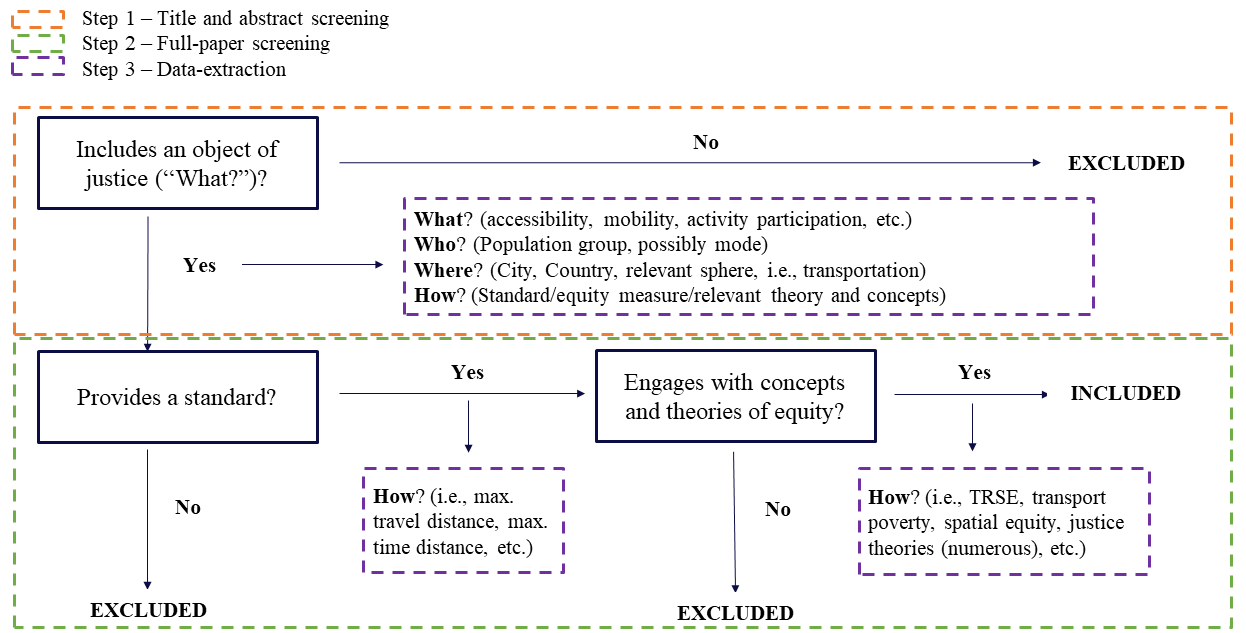
\includegraphics[width=4.15in,height=\textheight]{figures/Methods_framework.png}

}

\caption{\label{fig-fig1}Evidence selection process framework. Step 1
(orange) is title and abstract screening, step 2 (green) is full-text
review, and step 3 (purple) is data extraction.}

\end{figure}

The following steps summarize the process:

\begin{enumerate}
\def\labelenumi{\arabic{enumi}.}
\item
  The first step (orange box in Figure~\ref{fig-fig1}) included
  screening all titles and abstracts of papers on whether they included
  transportation equity as defined by the PCC. Each paper was screened
  by two independent reviewers who then voted for inclusion, exclusion,
  or uncertain inclusion. All uncertain papers, conflicting papers, and
  papers missing abstracts were reviewed by a third person for inclusion
  or exclusion.
\item
  The second step (green box in Figure~\ref{fig-fig1}) included scanning
  all full-text papers which passed step 1. These papers were reviewed
  to determine if they included a relevant ``how'', i.e., an standard
  and/or relevant theoretical or conceptual discussion. At this stage,
  papers were evaluated again by two independent reviewers who voted for
  inclusion or exclusion. If an article was voted to be excluded, it was
  tagged with one of five possible reasons for exclusion, namely (1) no
  standards included; (2) no relevant conceptual elements included; (3)
  no standard and no conceptual elements included; (4) send back -- QA
  issue; or (5) other. Discrepancies were resolved by a third reviewer.
\item
  In the last step, a data extraction template for each record was
  filled by one reviewer (purple box in Figure~\ref{fig-fig1}). The data
  extraction template was created with the aim of striking a balance
  between the complexity of categories and the simplicity of summary;
  information related to ``Where?'' (the geographical context and sphere
  of life), ``When?'' (temporal circumstances for the application of
  justice), ``Who?'' (the subject of justice), ``What?'' (the object of
  justice), and ``How?'' (equity standard(s) and concepts) was filled
  out for each study. Figure~\ref{fig-A2} contains the template that was
  input into \emph{Covidence} and used throughout.
\end{enumerate}

\begin{figure}

{\centering 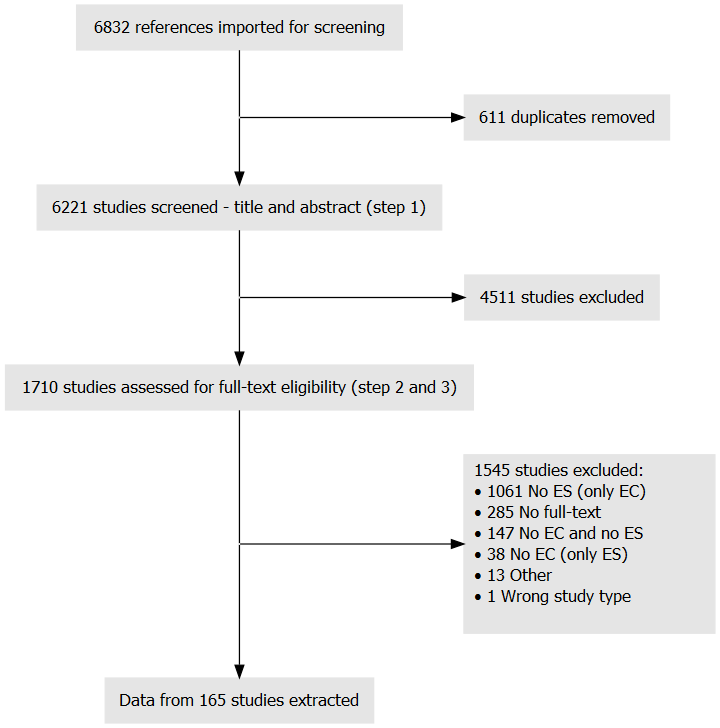
\includegraphics[width=2.4in,height=\textheight]{figures/Pflow_chart.png}

}

\caption{\label{fig-fig2}PRISMA flow diagram for the evidence selection
process. ES signifies equity standard and EC signifies equity
conceptualization.}

\end{figure}

The evidence selection process is also represented using the Preferred
Reporting Items for Systematic Reviews and Meta-Analyses (PRISMA) flow
diagram (Page et al. 2021) in Figure~\ref{fig-fig2}. Notably, two rounds
of exclusion occurred during the assessment for full-text eligibility.
1710 studies entered step 2, 1223 were excluded and the remaining 487
papers entered step 3. The data extraction template used by the
reviewers (authorship team) in step 3 revealed that, as expected,
inclusion was initially too generous, and some papers were not
sufficiently relevant, because of a lack of content on standards and/or
conceptual/theoretical elements. In this fashion, 322 papers were
further excluded and data extraction was completed to give a final
corpus of 165 papers. A summary of the reasons for exclusion of the 1545
papers (between steps 2 and 3) are included in Figure~\ref{fig-fig2}.

\hypertarget{sect4}{%
\section{The lay of the land: a summary of findings}\label{sect4}}

\begin{quote}
``\emph{Give me knowledge, so that I may have kindness for all.}''\\
--- Native American Proverb
\end{quote}

A synthesis of the findings from the data extraction process (based on
the template shown in Figure~\ref{fig-A2}) is detailed in this section.
The presentation of findings is less granular than the template to
highlight the key trends in the literature.

\hypertarget{when-and-where-the-context-for-justice}{%
\subsection{``When'' and ``Where'': the context for
justice}\label{when-and-where-the-context-for-justice}}

Figure~\ref{fig-fig3} displays the papers included in this review by
year of publication and geographical provenance. The literature related
to transportation equity has grown evidently voluminous, particularly
since 2019. Of note is the geographic scope of the relevant literature.
The majority of papers (60\%) contain case studies based in the Global
North, with many studies from North America (particularly USA and
Canada), Europe (particularly UK, France, Spain and Scandinavia),
Oceania (Australia and New Zealand), and Asia (Japan and Israel). For
the reasons previously discussed, setting standards (that is, making
statements of fairness) is a highly context-specific endeavor.
Publication patterns, being what they are, display a disproportionately
low number of items from the Global South where equity issues are
perhaps as, or even more pressing, than in the Global North (e.g., BBC
News, Latin America 2019). While our search strategy and review tries to
be as faithful to the literature as possible, it does not allow us to
lay claim to reporting about on-the-ground transportation justice
efforts from a truly global perspective.

\begin{figure}

{\centering 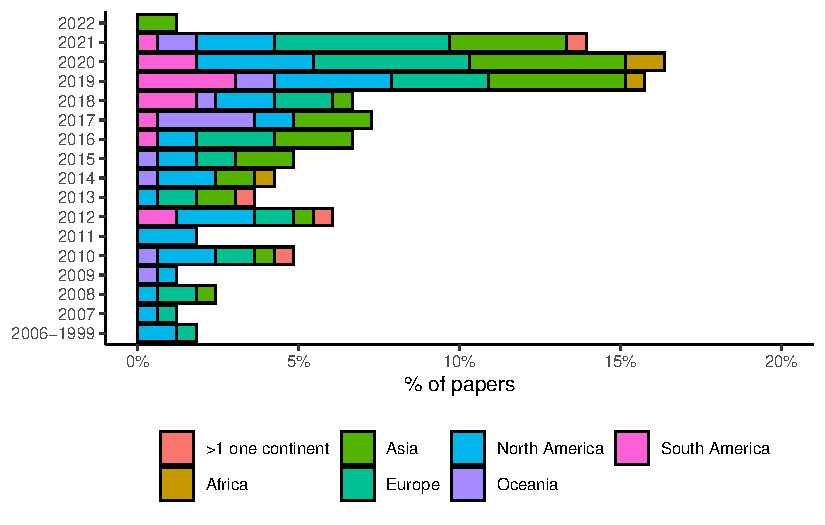
\includegraphics{just-transportation_files/figure-pdf/fig-fig3-1.pdf}

}

\caption{\label{fig-fig3}Papers included in the review by year of
publication and case study continent.}

\end{figure}

The smattering of studies from the Global South are predominately from
\textbf{Asia}, notably China, but also India, Thailand, Iran,
Philippines, and Indonesia. The next most common focus within the
literature from the Global South is from \textbf{South America}. Many of
these studies mention a systemic absence of evidence relevant to the
region (Vecchio, Tiznado-Aitken, and Hurtubia 2020). Despite the growing
recognition in the literature of the interconnections between transport
development, social exclusion, and poverty (Benevenuto and Caulfield
2020), a number of studies underscore an ongoing neglect of the social
dimension of transport during the planning stage (Benevenuto and
Caulfield 2020; Boisjoly et al. 2020). Many studies also point at
affordability as one of the main mobility barriers in the region
(Falavigna and Hernandez 2016; Rivas, Serebrisky, and Suárez-Alemán
2018), while some highlight multi-dimensional concerns such as public
transport accessibility and quality of walking environments that
contribute to mobility inequalities (Tiznado-Aitken, Munoz, and Hurtubia
2018).

Studies pertaining to \textbf{Africa} are even less numerous compared to
the South American literature. A shared characteristic among the studies
from these two continents is a scarcity of official transport data
(Fried et al. 2020) and a reliance on policy guidelines developed by
international organizations. These studies also incorporate the use of
informal transportation options and the pressures to develop road
network infrastructure (which tends to support car dependency) over
meeting the mobility/accessibility needs of citizens (Thondoo et al.
2020). To address these challenges, researchers compile databases based
on open and geo-referenced data, calculate objective and/or subjective
measures (Berhe, Martinez, and Verplanke 2014), and focus on advancing
transport justice for low to medium income countries (LMIC) by aligning
their goals with external policy guidelines such as the Sustainability
Development Goals (SDGs), particularly those related to universal
accessibility (Fried et al. 2020).

Of all the studies reviewed, 85\% focus on urban and suburban settings
and are highly varied in their research aims. To give an example, Cox
and Bartle (2020) qualitatively examine cycling as a mode of travel for
people with disabilities in a typical mid-size town in the UK. Ampe et
al. (2020), on the other hand, work to identify the lateral clearance
that motorists should maintain when passing cyclists with children
seats. While both studies refer to the same objects of justice
(``what'', i.e., the right to the road and cycling), the subjects of
inequities (the ``who'') are different (people with disabilities and
children), and the ``where'', that is, the geographical context for the
examination of fairness, differs as well.

The remainder of the studies reviewed focus on rural regions (14\%). To
illustrate, we highlight the work of Cao and Stanley (2017), who
examined transportation disadvantage in remote places which rely on
inter-island ferry trips in the rural Philippines. Similarly, Parry et
al. (2018) studied remote communities in the Amazonian region, and
suggest that ``increasing accessibility through road building would be
maladaptive, exposing marginalized people to further harm and
exacerbating climatic change by driving deforestation'' (pp.~125).

\hypertarget{who-the-subjects-of-justice}{%
\subsection{``Who'': the subjects of
justice}\label{who-the-subjects-of-justice}}

Figure~\ref{fig-fig4} showcases the population group types that are the
focus of the papers in our review. From this tally, papers that consider
population by income groups are the most widely represented in the
literature reviewed. Particularly, most papers that center income
usually focus on the lowest-income groups, as they experience the least
benefits in terms of mobility and accessibility, and usually the
greatest burdens as well, in terms of cost, exposure, and so on
(Peungnumsai et al. 2020; PJ Zhao, Li, and Liu 2020; Falavigna and
Hernandez 2016).

\begin{figure}

{\centering 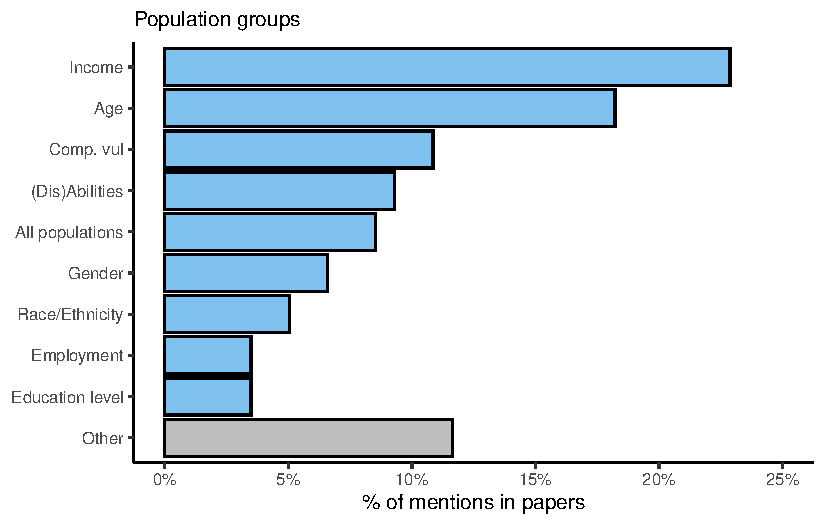
\includegraphics{just-transportation_files/figure-pdf/fig-fig4-1.pdf}

}

\caption{\label{fig-fig4}The proportion of papers that focus on each
type of population group. Categories for population groups were
generated upon data extraction.}

\end{figure}

For example, there is an abundance of evidence to suggest that
low-levels of household income is a significant determinant of
transport-related inequities (e.g., access to public transport supply in
Bangkok region (Thailand) (Peungnumsai et al. 2020), access to
employment opportunities in various cities in Brazil (Boisjoly et al.
2020), and unfavorable rates of environmental noise, air pollution, and
green space per resident in Rijnmond region (Netherlands) (Kruize et al.
2007). However, this should be kept in context, as low-income is not
universally associated with lower transport-related benefits for every
object of justice. For instance, in Sheffield (UK), Mears et al. (2019)
demonstrates that historically working-class neighbourhoods (i.e., lower
income working population) have more access to green space than other
neighbourhoods due to urban planning approaches during the
Victorian-era. However, the quality of green spaces are less than
average. Similarly, Bertrand, Therien, and Cloutier (2008) finds that
lower income groups do not always have below average accessibility
depending on the granularity of analysis (i.e., the distance-to-food
threshold for the cumulative opportunity measure).

Age is the second most common category of population group of focus
within the reviewed literature. Many papers that focus on this category
highlight differences in age-related capabilities; for instance,
Martinez-Jimenez and Salinas-Perez (2019) and Arranz-Lopez, Soria-Lara,
and Pueyo-Campos (2019) investigate travel distances and times to
various opportunities based on specific age groups, acknowledging that
age is an important consideration, and associated with differences in
access to opportunities. The most commonly studied age groups are
school-aged children and older populations. Research on school-aged
children analyzes their wellbeing (Laszkiewicz and Sikorska 2020),
exposure to green space (Corazza et al. 2020), access to schools (Sharma
and Patil 2022), and aims at understanding and encouraging active travel
journeys (Mackie 2009; Mehdizadeh, Mamdoohi, and Nordfjaern 2017).
Papers that focus on older adults often have similar aims as those on
children, and try to understand transport-related impacts on wellbeing
(e.g, Y. Chen et al. 2020), measuring accessibility to key destinations
by population group (e.g. Cheng et al. 2019), and seeking to understand
how to better meet travel needs (e.g., Nordbakke and Schwanen 2015).

The third population group most commonly studied is what might be called
`composite vulnerable population groups': the intersection of several
individual traits. These papers use composite vulnerability indices that
captures multiple population characteristics, including low-income,
unemployment, immigrant status, family household characteristics, and so
on. These indices are typically generated from official government
sources or author-informed census data creation, and produced using a
variety of methodologies. For instance, Awuor and Melles (2019) use the
Neighbourhood Equity Index (NEI) to investigate disparities in premature
death in Toronto (Canada). The NEI is a composite index that was
developed by the city to capture differences in the City's
neighbourhoods by ranking them based on socio-economic characteristics
(e.g., social assistance, unemployment, income) and physical
environmental characteristics such as green space availability. Other
works use national census indicators such as the social and housing
deprivation index {[}e.g., Pucci et al. (2019) or explore transport
disadvantage, equity in policy implementation, or transport-related
mortality burden by means of census measures (e.g., household poverty)
and transport-related indicators {[}e.g., accessibility; Aldred et al.
(2021); Iungman et al. (2021); Sun and Thakuriah (2021); Scheurer,
Curtis, and McLeod (2017){]}. Similarly, Environmental Justice (EJ)
indicators have been used in the US literature to identify
neighbourhoods that have a higher than average proportion of low-income
and non-white populations (i.e., a composite vulnerable population
group'). Numerous studies have used EJ analysis to evaluate the equity
impacts of transportation projects (e.g., D. Rowangould, Karner, and
London 2016; K. Park et al. 2021; Reddy, Chennadu, and Lu 2010).

Papers that exclusively focus on populations with (dis)abilities e.g.,
(J. Park et al. 2017; Chiscano 2021; Orellana et al. 2020) are
relatively common in the literature. They often assess universal design
guidelines and the capabilities of people who face disabilities to
travel. However, from another perspective, papers with an exclusive
focus on gender, race/ethnicity, or education level/employment are less
common in the literature reviewed. Only two papers focus on gendered
differences in cycling/active transportation (e.g., Adlakha and Parra
(2020)`s case study in Chennai (India) and Xie and Spinney (2018)'s case
study in Cardiff (UK)). Only two papers focus on race/ethnicity
exclusively focusing on how minority ethnicity communities are in
proximity to green space (Silva et al. 2018) and culturally diverse
family physicians in Toronto (Canada) (Wang and Roisman 2011).
Furthermore, papers that focus \emph{solely} on education/employment
status are not present in the reviewed papers. This is to say, papers
that feature gender, race/ethnicity, or education level/employment
population groups often feature them alongside other population group
characteristics (as a trait in 'composite vulnerability measures'). This
contrasts the prominence of studies that exclusively center on
disabilities.

We include a catch-all category of papers (\emph{Other}) that include
group populations that less commonly have been the subject of research.
Examples include: veterans and access to specific-healthcare needs
(Mooney et al. 2000), pregnant people and access to services (Vadrevu
and Kanjilal 2016), and youths who live in foster care (Batsche and
Reader 2012). Overall, the diversity of the \emph{Other} population
group classification demonstrates the diversity of transportation-equity
concerns across population groups in the reviewed literature and the
interplay of characteristics in the literature (Vecchio et al. 2022).

\hypertarget{who-and-what-the-tools-of-mobility}{%
\subsection{``Who'' and ``What'': the tools of
mobility}\label{who-and-what-the-tools-of-mobility}}

\begin{figure}

{\centering 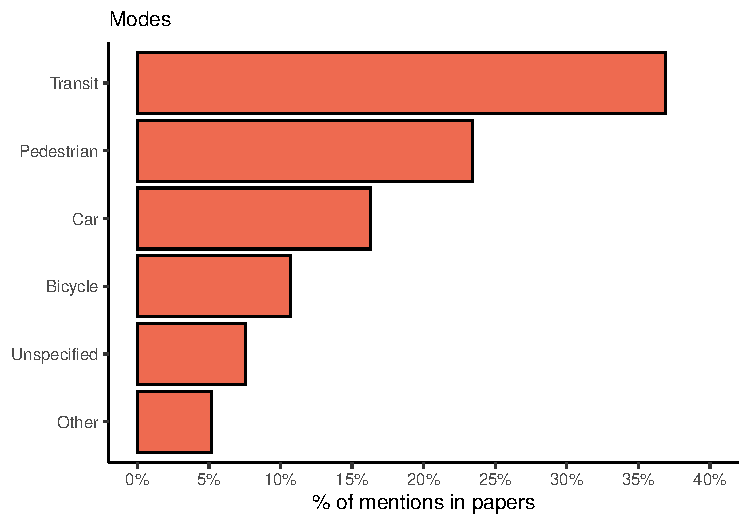
\includegraphics{just-transportation_files/figure-pdf/fig-fig5-1.pdf}

}

\caption{\label{fig-fig5}The proportion of papers that investiage each
type of mode. Categories for modes were generated upon data extraction.}

\end{figure}

As previously noted, mode of travel is not a trait of the individual,
but in principle is a modifiable factor. That said, the existence of
captive users by mode makes it challenging at times to extricate the
mobility tool from the individual. In this section, we choose to view
the mode of travel primarily as an object of justice (i.e., a ``what''),
but occasionally this will be enjoined to the subject of justice (i.e.,
the ``who'').

It is interesting to note that the primary emphasis within the
literature reviewed centers on public transit (Figure~\ref{fig-fig5}), a
mode that often is perceived by users as less than ideal (A. Paez and
Whalen 2010; Mella Lira and Paez 2021) and that yet is often reckoned as
the only realistic mobility tool for many (Jacques, Manaugh, and
El-Geneidy 2012; T. F. Welch and Mishra 2013; Cheranchery and Maitra
2018). The variety of topics assessed from the perspective of public
transit are varied. For instance, McKey, Kim, and Seo (2020) identifies
`food deserts' in Dallas (USA) considering public transit accessibility.
Other contributions intersect public transport and individual needs.
Examples include the study of universal design and barrier-free
transportation for people who face disabilities (e.g., Jiménez-Espada
and González-Escobar 2021; Liu et al. 2019) or possible improvements to
public transport for people with autism (Lim et al. 2021; Feeley 2019).
The strong focus on public passenger transport systems could be due to
their policy importance. They are a clear public good, and seen as a
natural object of justice. Accordingly, public transportation is seen as
adaptable to meet the demands of justice, for example by funding it
sufficiently to provide barrier-free transport for most. In this
respect, the literature points at a variety of factors that conspire
against it, including low population and opportunity density (the
outcome of decades of deliberate policy choices), fiscal prudence (the
public face of the choice to lower taxes), and political will {[}to
maintain or further unsustainable socio-technological systems, from SUVs
to space tourism; Markard et al. (2023){]}.

Transit is also often central to multi-modal or holistic comparisons
that may serve transport equity analysis. As an example, Brussel et al.
(2019) compares three different approaches to measure accessibility in
the context of the Sustainability Development Goals (11.2) for the case
of Bogota (Colombia), all of which capture some/all of the public
transit system while others capture road and/or pedestrian systems. From
a different perspective, Renne and Mayorga (2018) reviews natural
disaster emergency evacuation plans from the lens of car-less (and
oftentimes vulnerable) households in regions across the USA, paying
particular attention to transit and pedestrian networks.

In contrast, only a few papers in the literature frame transit as a
`car-free' option and compare transit to car access. This framing is
notable as car travel can be seen as a direct competitor to transit or
as a benchmark for travel times and accessibility levels (Golub and
Martens 2014; K. Martens, Golub, and Robinson 2012). As an example,
Warren et al. (2015) propose a standard for per capita car ownership for
Havana (Cuba), in recognition that car mobility is needed to alleviate
transportation disadvantage in the short-term where public transit has
yet to be sufficiently addressed. In this context, Warren et al. (2015)
acknowledge the tension between household vulnerability and their need
for mobility against GHG emission reduction goals and car-dependency
cycles. However, not all papers see transit as a direct competitor, but
as a mode that can be used to satisfy individual capabilities. For
instance, Smith, Hirsch, and Davis (2012) focus on rural areas in the UK
and various types of households (e.g., retired, no-children, with
children, single, etc.). In this investigation, perspectives about
minimum transport needs and costs for a variety of living standards are
explored. The papers reviewed vary in the importance they place on
climate urgency, with some focusing more on satisfying \emph{all}
sufficient individual needs while planning for less car-dependent cities
in the future.

Following a focus on transit, a focus on pedestrian travel is the second
most common object of justice considered in the literature. Pedestrians
are the most extreme case of confluence between the ``what'' and the
``who'', since the mobility tool is the person's own body, with its
inherent range of abilities. In papers that focus exclusively on
walking, many use or develop walkability scores to explore perceptions
of neighbourhood quality (Evans 2015) or pedestrian mobility with a
focus on middle-aged and older adults (Towne et al. 2016), gender (H.
Kim et al. 2016), or urban peripherical regions (Blecic et al. 2021).
These papers use `walkability' as a way to measure the equity in its
distribution. Other papers use walkability as an indicator for public
health and urban vitality (Sung and Lee 2015; McCormack et al. 2012).

Additionally, papers that focus on pedestrians also often see walking as
a bridge to connect multiple modes: they often discuss `walkability' as
part of active transportation, which focuses on both walking and bicycle
and/or transit. Concepts discussed include how active transport
contributes to children's physical activity levels (Mammen et al. 2014),
walkability as an alternative to car predominance (Bertrand, Therien,
and Cloutier 2008) or tension that exists between modes, creating unsafe
conditions for walking (Siu 2019; Ferenchak and Marshall 2019).

In contrast to transit and walking, cars are seldom the only mode
examined within a paper. When car as a mobility tool is studied, it is
often used as a comparison with transit or as the only mode of transport
for areas with sub-standard transit systems e.g., (Kimmel et al. 2018;
Aljoufie 2016). Similarly, a number of car studies focus on
externalities such as air pollution or safety (Tao Feng and Timmermans
2014; Houston et al. 2006).

\hypertarget{what-the-benefits-of-mobility-and-accessibility}{%
\subsection{``What'': the benefits of mobility and
accessibility}\label{what-the-benefits-of-mobility-and-accessibility}}

The most fundamental benefits of transportation systems are mobility
(enabling or impeding movement) and accessibility (the ease of reaching
destinations). These benefits, however, are not necessarily valued by
themselves, but rather are seen as instrumental to achieve an ulterior
goal (e.g., activity participation). For example, although vehicle
kilometers travelled (VKT) is still sometimes seen as a useful policy
instrument (Pengjun Zhao and Li 2021), travelling more is not
necessarily a sign of advantage when accessibility is low (A. Paez et
al. 2010), and similarly short trips may be a sign of advantage (K. Park
et al. 2021). For this reason, although the right to the road (and to
transportation systems more generally) is important, the literature
leans heavy on the ulterior object, namely accessibility to
destinations.

In this respect, we find that most papers tend to be wide sighted, in
that they do not focus on a particular destination (e.g., 28\% of
studies). Within these papers, a variety of equity dimensions, often in
combination with different modes of transportation. Typically, they are
multi-modal and focus on factors that impact the \textbf{trip itself}
(e.g., the trip experience, the quality of infrastructure, the level of
service) or on the \textbf{people and relevant destinations that can be
accessed} (e.g., a bundle of trips made by specific population groups,
and whether they are enough for `sufficient' quality of life). For the
first, the focus is on the quality of infrastructure, safety issues,
perceived accessibility and facets of the level of service such as
frequency (Zhe et al. 2008; Prasertsubpakij and Nitivattananon 2012;
Fürst and Vogelauer 2013 ; Lattman, Friman, and Olsson 2016). For the
second, the focus is on bundles of trips tailored for specific
population groups, such as women (Russell et al. 2021) or people who
face physical disabilities (Wilkinson-Meyers et al. 2015). More broadly
there is the question of what is enough for the quality of life to be
`sufficient' (Churchill and Smyth 2019). These papers further
demonstrate the multi-dimensional role of transportation systems: they
provide a utilitarian service that can be used to get from A to B but
they too are experienced by the people that use them. Papers that
examine `all trips' best exemplify this trend in the transportation
equity literature.

In terms of papers that study specific destinations, healthcare services
(11\%) and employment (15\%) are activities commonly studied. Papers
that exclusively focus on healthcare typically originate from the
healthcare planning literature, and look to inform planners about
disparities in services and corrective actions. For instance, Wang and
Roisman (2011) model access of Chinese-language speakers in Toronto
(Canada) to Mandarin-speaking family physicians. These authors infer an
inequity from the spatial mismatch between language competent healthcare
providers and Chinese speakers. Papers that exclusively focus on
employment typically focus on these trips as they are the most common
trip purpose and are often correlated with other trip activities like
shops, recreation, and other services. For instance, J. Allen and Farber
(2019) propose a low employment-based accessibility threshold and a
composite population vulnerability index to identify transportation-poor
neighbourhoods in urban Canada. Papers that focus on healthcare and
employment typically source data from representative travel
surveys/diaries, census data, and points-of-interest databases. In other
words, these studies often benefit from well developed and institutional
data that represents `typical trips', especially in the Global North
where these data are more readily available.

But what about non-healthcare and non-employment activity types? Papers
that focus on other activities are not framed as `typical travel
patterns' and they often have different intentions. For instance, papers
that focus on shopping destinations, such as grocery stores or markets
(12\%), frequently aim to identify food deserts (e.g., Choi and Suzuki
2013; Jiao et al. 2012; McKey, Kim, and Seo 2020; D. Kim and Park 2020).
Papers that focus on educational facilities, including primary,
secondary, and post-secondary schools, represent only 11\% of the
studies, and examine children's active transportation to school (e.g.,
Laszkiewicz and Sikorska 2020) or universal design (e.g., Larkins,
Dunning, and Ridout 2011). When green space or other places of leisure
is the exclusive focus (11\% of papers), studies examine different
accessibility questions such as the spatial distribution of green space
e.g., (Xu et al. 2017), for whom its accessible to (e.g., Mavoa et al.
2015), and the reasons why the distribution of these spaces may be
unequitable (e.g., Mears et al. 2019). Very few of the papers we
reviewed include `community' destinations (e.g., public service centres,
places of community support, and places of worship (6\% of studies) or
childcare activity types (3\% of studies). In the few papers that do
include them, these destinations are considered in a holistic
representation of activity participation (Alberts, Pfeffer, and Baud
2016; Smith, Hirsch, and Davis 2012). The lack of information about
community destinations is particularly pronounced in the case of
children, as per Elise Desjardins et al. (2022).

The literature offers a variety of conclusions and recommendations that
span across the benefits of transportation (e.g., destinations types),
often co-mingled with population groups and the tools of mobility. In
addition, as we will discuss next, there is a variety of perspectives in
terms of the philosophical foundations and the standards of fairness.

\hypertarget{how-concepts-of-justice-and-standards-of-fairness}{%
\subsection{``How'': concepts of justice and standards of
fairness}\label{how-concepts-of-justice-and-standards-of-fairness}}

\begin{figure}

{\centering 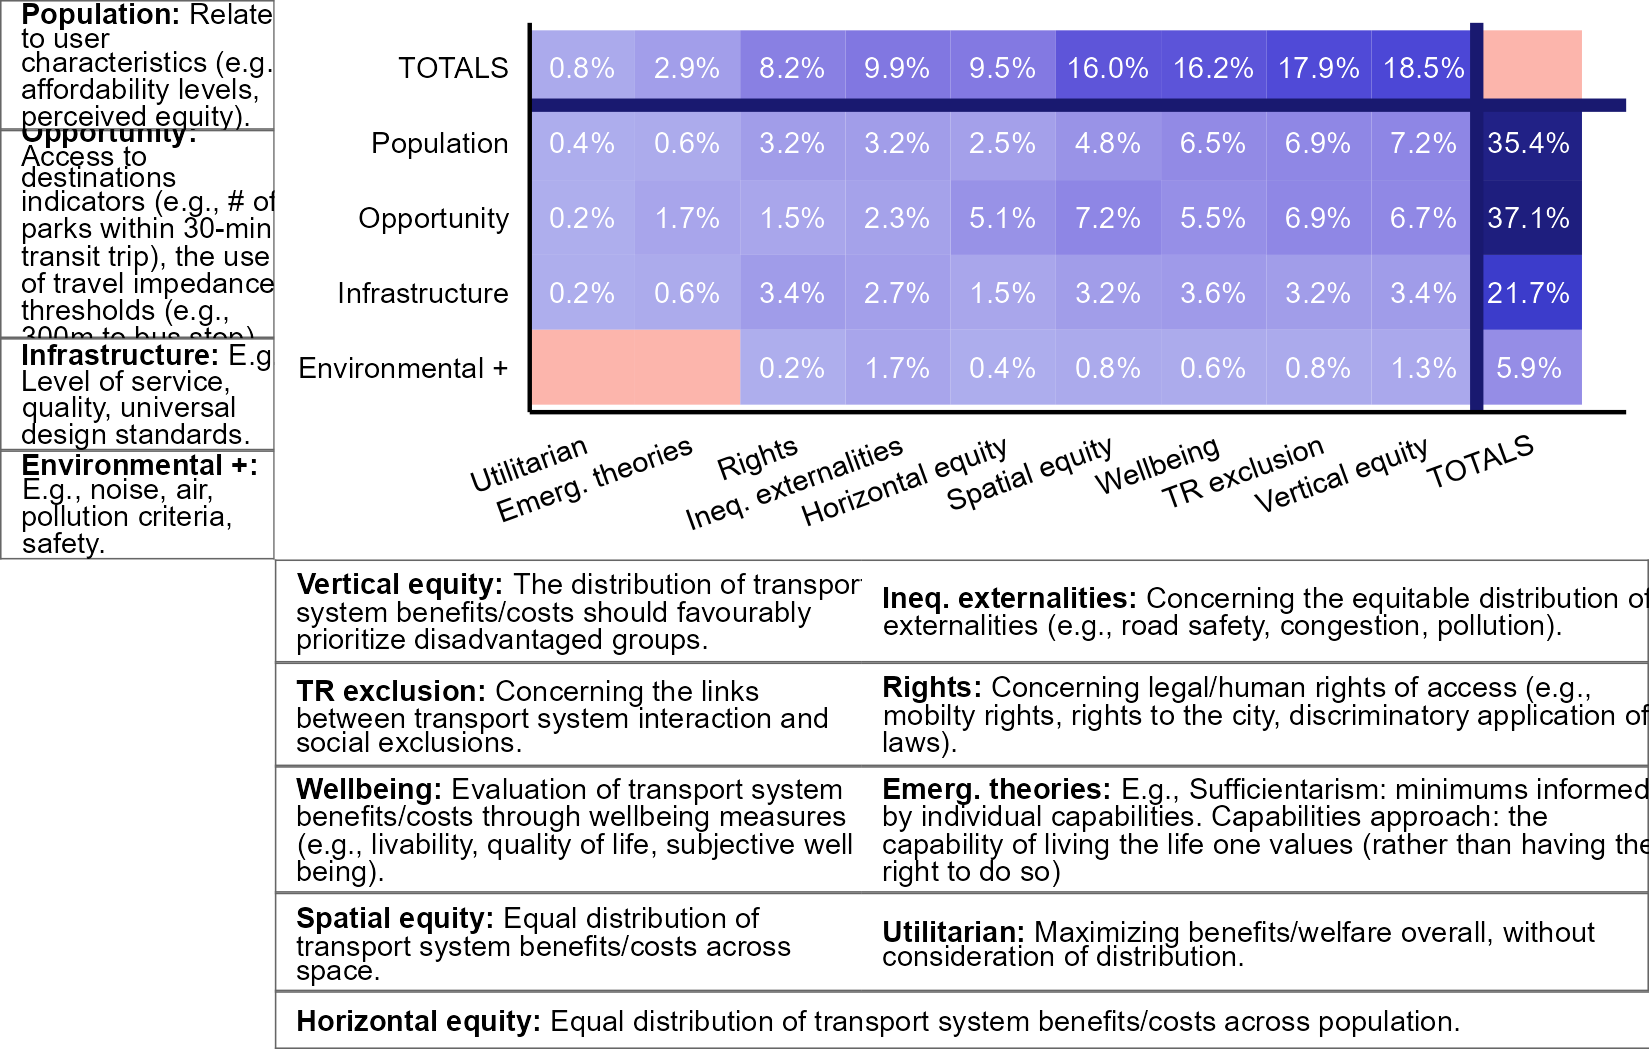
\includegraphics[width=5.5in,height=\textheight]{figures/standards_conc_percentages_plot_and_table.png}

}

\caption{\label{fig-fig6}The proportion of equity standards (vertical
axis) within each type of equity conceptualization (horizontal axis)
category.}

\end{figure}

We begin this section with our reflections about the way equity
standards connect with conceptual and theoretical frameworks of justice.
Broadly speaking, some trends emerge in terms of the methods used
depending on the way equity is conceptualized and the type of standard
suggested; See Figure~\ref{fig-fig6} for definitions of of
conceptualizations along the horizontal axis and types of standards
along the vertical axis. These categories emerged as we reviewed the
literature and we use them to discuss trends; they are by no means an
exhaustive list of equity conceptualizations and types of standards.

Referring to Figure~\ref{fig-fig6}, \textbf{Opportunity} and
\textbf{population} are the most commonly suggested standards in the
literature reviewed; they appear in the literature in similar
proportions ( 37.2\% vs.~35.8\%), but frequently correspond to different
conceptualizations of equity. Papers suggesting \textbf{opportunity
standards} often address questions of \textbf{horizontal equity} and
\textbf{spatial equity} and suggest standards that relate to travel
impedance; these standards describes how fast, far, or costly it is to
travel from one place to another. We think of this as a type of
opportunity standard because travel impedance is essential to the
measurement of accessibility (i.e., the ease of reaching opportunities).
Some examples include the work of Z. Chen and Haynes (2017), who uses a
standard of 4 hours or less by high-speed rail for municipalities to be
considered ``comfortably connected''. In a similar manner, Yenisetty and
Bahadure (2020) assumes that a travel distance of less than 1,200 m is
sufficient for a resident to interact with its transit system locally.
And Shen et al. (2020) identify regions where populations cannot access
hospitals within 1 hour by car - in other words, more than sixty minutes
travel time is already seen as an unfair burden. These papers uses these
standards as a benchmark to indicate what areas are better or worse-off
in terms of travel impedance; we can interpret them to be a type of
\emph{difference} threshold.

Papers that suggest these \textbf{opportunity} standards sometimes also
employ disparity analysis through a variety of quantitative approaches
to discuss the fairness in distribution. These include inequality
measures such as the Gini coefficient and Lorenz curve, or poverty
measures e.g., (van der Veen et al. 2020; Tiznado-Aitken, Munoz, and
Hurtubia 2018)). They can also include spatial descriptive analysis as
well as comparisons to service benchmarks (e.g., equal supply to demand
of public transit in a spatial unit as in Peungnumsai et al. 2020) to
determine which locations are spatially and horizontally (in)equitable.
Another branch of opportunity-standard-suggesting papers conceive the
externalities of transportation system as trade-offs, and aim to
maximize transport-related benefits (i.e., time savings, emissions
reductions, congestion reductions, user fares) through
optimization/location-allocation methodologies e.g., (T. Feng and Zhang
2014; Fakhrmoosavi, Zockaie, and Abdelghany 2021; Zheng and Geroliminis
2020; Wismadi et al. 2014). In the reviewed papers that focus primarily
on \textbf{horizontal equity} and/or \textbf{spatial equity} seldom use
exclusively qualitative methods and operationalise predominately
quantitative methods.

A different way to approach standards is to see them from the lens of
\textbf{population}, and when this is done, other methods are commonly
used, often depending on how equity is conceptualised. Papers that
suggest \textbf{population}-based standards are often founded on
concepts of \textbf{well-being}: they typically ask \emph{what is enough
to lead a satisfactory life (as related to transportation)?}. Standards
suggested include: questionnaires and relative comparisons to
recommended physical activity per week e.g., (Adlakha and Parra 2020;
Auchincloss et al. 2020; McCormack et al. 2012; H. Kim et al. 2016;
Towne et al. 2016), summative per capita benchmarks (e.g., such as
energy consumption for a `decent living' as suggested in Rao and Baer
(2012)), region-relative comparisons in health-related outcomes (e.g.,
premature mortality rates (Awuor and Melles 2019)), spatial access
benchmarks to hospitals e.g., (R. Pereira et al. 2021), as well as
spatial access to supermarkets, active-mode-usage, and Body Mass Index
(BMI) e.g., (Murphy et al. 2017). The majority of these papers use
quantitative/mixed-methods to identify inequities in \textbf{wellbeing}.
However, a minority do use exclusively qualitative methods to distill
themes, as for example in the exploration of perceived quality of life
by Berhe, Martinez, and Verplanke (2014).

Papers that combine \textbf{population}- and \textbf{opportunity}-based
standards often rely on \textbf{vertical equity} and
\textbf{transport-related social exclusion} (note the similar
proportions in these standards in Figure~\ref{fig-fig6}). Perhaps not
surprisingly, these papers commonly use a combination of methods:
questionnaires and other qualitative methods related to population
standards and quantitative methods such as accessibility indices for
opportunity standards are usually deployed. For instance, census data
and the estimated proportion of households within some travel
distance/time/availability to/of key destinations is used to identify a
variety of social exclusionary situations e.g., (Mackett, Achuthan, and
Titheridge 2010; W.-H. Chen 2010; Daniels and Mulley 2011; Sun and
Thakuriah 2021; Sharma and Patil 2021), the linkages between well-being
and transport-related social exclusion e.g.,(A. Delbosc and Currie
2011b; Churchill and Smyth 2019), areas more likely to experience
transport poverty (J. Allen and Farber 2019), food deserts (McKey, Kim,
and Seo 2020), or transport-related energy poverty e.g., (Robinson and
Mattioli 2020; Berry et al. 2016; Berry 2019).

Similar to papers interested in \textbf{wellbeing}, the majority of
papers concerned with \textbf{social-exclusion} use
quantitative/mixed-methods to identify areas, households, and/or
populations at risk. They use a variety of methods to identify
\emph{where} populations at risk may be located, such as clustering
methods (Mohri, Mortazavi, and Nassir 2021). Some papers that
exclusively use qualitative methods operationalise survey data to study
the willingness/barriers to travel e.g., (W.-H. Chen 2010; Mehdizadeh,
Mamdoohi, and Nordfjaern 2017) or conducts interviews on topics of unmet
activity needs (Nordbakke and Schwanen 2015). Travel that \emph{did not}
take place is notoriously slippery to capture in standard surveys, and
understanding whether this is a preference or the consequence of
constraints is not straightforward (e.g., A. Paez and Farber 2012).

Besides \textbf{opportunity}- and \textbf{population}-based standards,
another way to create statements about fairness is through
\textbf{infrastructure}-based standards. Among papers that use this
lens, the most common conceptual grounding used relates to
\textbf{rights}. \textbf{Infrastructure}-standards appear in 37\% of all
papers in this review, and within this segment of the corpus,
discussions of \textbf{rights} appear two times as often than any other
conceptual approach. These papers often focus on populations who face
mobility disabilities and non-car users, and the discussion often
centers on their right to use existing transportation systems. The
methods operationalised by this strand of the literature are varied but
are more or less split between infrastructure and environmental audits,
and qualitative methods. Audits of existing infrastructure are sometimes
used in comparisons against best-practice universal design e.g., (Odeck,
Hagen, and Fearnley 2010; Larkins, Dunning, and Ridout 2011;
Jiménez-Espada and González-Escobar 2021; Perez-delHoyo et al. 2021) or
to understand the elements of infrastructure that correlate well with
use of a mode by particular populations (e.g., walking by older adults
Moniruzzaman and Paez 2016). Qualitative methods are used to
interview/survey users about their perceived access to transport systems
(e.g., Marquez, Poveda, and Vega 2019; Iderlina Mateo-Babiano, Kumar,
and Mejia 2017; Fürst and Vogelauer 2013; Velho et al. 2016; J. Park et
al. 2017; Lim et al. 2021; Stjernborg 2019; Elise Desjardins et al.
2021) or to assess standards under best-practice considerations (e.g.,
Daamen, de Boer, and de Kloe 2008; Velho et al. 2016; Bharathy and
D'Souza 2018).

Papers that suggest \textbf{infrastructure}-based standards are also
sometimes multi-dimensional, and extend beyond \textbf{rights} (to the
infrastructure) to suggest \textbf{opportunity}- and
\textbf{population}-based standards as well. These papers often apply
\textbf{vertical}, \textbf{horizontal} and \textbf{spatial} equity
lenses. Papers in this slice of the literature can refer to established
guidelines and suggest composite indices. For instance, Rachele et al.
(2017) combine various properties of transport networks (e.g., street
connectivity, cul-de-sac length, street block length, traffic volume,
public transport stops and service frequency), and use these attributes
as inputs to define an indicator of transport design that supports
walkability and access to public transport. Other works assess the
quality of infrastructure (Xu et al. 2017), the severity and frequency
of accidents on the system (Benevenuto and Caulfield 2020; Appleyard,
Ferrell, and Taecker 2017), user-groups (particularly disadvantaged
groups in the case of vertical equity conceptualisations)
(Prasertsubpakij and Nitivattananon 2012) as part of multi-criteria
indicators. Yet another branch of infrastructure-based
standard-suggesting literature explicitly focuses on affordability or
other barriers to the transport system, and suggests improvements to the
infrastructure such that all groups (especially the most disadvantaged)
can sufficiently interact with the system (e.g., Basu and Alves 2019;
Song, Kirschen, and Taylor 2019; T. Welch 2013). These studies are
grounded on concepts of \textbf{transport-related social exclusion}
(e.g., Kent and Karner 2019) or \textbf{sufficientarian/capabilities}
approaches (e.g., Smith, Hirsch, and Davis 2012).

Our corpus of literature was more or less muted in terms of studies with
\textbf{environmental}-based standards (only about 4\% of all papers).
Of those papers, the most frequent focus is on \textbf{inequitable
externalities}. This paucity in our corpus could be due to the fact that
the the environmental burdens of transportation are covered more broadly
in other literatures (e.g., environmental justice). Papers that work
with environmental-based standards often use traffic-related air
pollution, noise pollution, green-space, urban design elements, urban
air temperature, health related outcome, and physical activity
guidelines to quantify externalities. The methods used are almost always
quantitative or mixed-methods, and inequalities are identified using
spatial clustering techniques, Gini coefficients (T. Feng and Zhang
2014), comparisons to established environmental thresholds or health
guidelines (Agost-Felip, Rua, and Kouidmi 2021, 2021; Kruize et al.
2007; Iungman et al. 2021; Apparicio et al. 2021; Khomenko et al. 2020;
Mueller et al. 2018). They sometimes create composite multi-dimensional
indices (Agost-Felip, Rua, and Kouidmi 2021; Miranda and da Silva 2012;
Corazza et al. 2020), occasionally supported by spatial analysis
(Jephcote and Chen 2013; Carrier et al. 2014).

See the final table in the appendix that presents detailed examples of
various standards as retrieved from our corpus.

\hypertarget{sect5}{%
\section{A critical appraisal of the lay of the land}\label{sect5}}

\begin{quote}
``\emph{Justice is itself the great standing policy of civil society;
and any eminent departure from it, under any circumstances, lies under
the suspicion of being no policy at all.}''\\
--- Edmund Burke
\end{quote}

Here, we critically review some of the trends identified from the
literature in terms of concepts and standards (the ``how'') and how they
apply to the objects (the ``what'') and subjects (the ``who'') of
justice, as well as under which situations (``when'' and ``where'').

\hypertarget{when-and-where-is-transportation-considered-a-sphere-of-justice}{%
\subsection{``When'' and ``Where'' is transportation considered a sphere
of
justice}\label{when-and-where-is-transportation-considered-a-sphere-of-justice}}

Most papers within our corpus (60\%) focus on case studies in the Global
North. Though their subject matter is varied, their spatial context
mainly pertains to North American and Europe, and thus more often than
not, in conversation with more developed and formal government transport
planning apparatuses and technologies (e.g., planning for equitable
high-speed rail, as in Monzon, Ortega, and Lopez 2013; autonomous
vehicle technology, as in Eppenberger and Richter 2021; or on the public
consultation processes, as in Reddy, Chennadu, and Lu 2010)).

However, studies from the Global South, specifically South America and
Africa, have key differences in focus compared to the Global North.
Three emerge from our review: 1) affordability-as-a-barrier is often
what motivates them; 2) the tension between investing in new
transportation infrastructure (typically roads) or prioritizing other
modes; and 3) more serious data availability limitations. In this way,
work from the Global South does not engage as immediately with emerging
mobility technologies that have large capital costs. Informal aspects
present in transport planning are a more overbearing presence. In the
present day, countries in the Global South still struggle with the
consequences of past colonialism under Northern states. This has left
them more heavily reliant on primary sector exports (lower efficiency,
lower national GDP) under growing global financial markets, and with
more fragile democracies. Because of lower data availability and more
extreme needs for `sufficient' transport, analysis of transportation
inequities are often cast along economic lines. An example of a standard
in this context involves improving transit to ensure that at least 60\%
of those below the poverty line face a similar burden travelling to
work, school, and services, as the average transit user in the region
(i.e., 60 min travel time to destinations Basu and Alves 2019).

Temporally, we see the literature from the Global North and Global South
in our corupus as laying on different transport inequity continuums.
Literature from the Global North is concerned with particularly
disadvantaged groups and creating indicators that may be used to guide
the remedy of formal processes that ensure access to societal benefits
e.g., (Cui et al. 2020). Global North countries often surpass
international sufficiency thresholds related to transport and public
health (e.g., Carrier et al. (2014) measures NO\_\{2\} road-side air
pollution and find no levels are below the WHO guidelines) but advocate
for the reduction in disproportional impact of air pollution on
lower-income groups. These international guidelines, while perhaps being
relevant at a time of lower transport-related development, are no longer
relevant for some areas in the Global North. Along this line, inequities
in the Global North are rising - high-income countries contain the
wealthiest populations that have the most mobility (and produce
associated carbon externalities) (Chancel and Piketty 2015).

In reference to transport inequity continuum, literature from the Global
South tend to operationalize international standards as guidelines.
Though not covered in this review, Global South nations' formal
processes for planning are newer (relatively), more fragile, and
operating under more strict financial constraints than the Global North.
Informal processes are thus more important to account for equity (e.g,
informal transit (Fried et al. 2020), populations living in informal
residential locations (Sharma and Patil 2021)). Comparisons to
thresholds set by governing international bodies are relevant as
minimums are relatively lower (e.g., traffic related pollution, access
to basic healthcare). Global South, along some dimensions, are lagging
Global North development, but have the opportunity to plan better and
not repeat Global North mistakes (e.g., car-centric development (Warren
et al. 2015)).

So what's missing from the answers to ``Where?'' and ``When?'':
standards that are context-specific, particularly those that frame the
disproportionate impacts of inequities on both disadvantage groups and
the most advantaged. Inequities in the Global North and Global South are
broadly different as a result of globalizing forces, but systems
thinking is required to advocate for equity standards that re-balance,
develop, and uphold equitable formal transport planning processes.

\hypertarget{who-are-the-subjects-of-transportation-justice}{%
\subsection{``Who'' are the subjects of transportation
justice}\label{who-are-the-subjects-of-transportation-justice}}

Though the literature reviewed most commonly considers low-income as a
socio-demographic characteristics of populations deserving equity as
either by itself or alongside other characteristics (11.08\% of the
papers). Many employ accessibility methods (e.g., walking accessibility
to open space (Tang et al. 2021)) but others use qualitative or
mixed-methods to gain perspectives of inequalities that are typically
cross-dimensional (e.g., Milan and Creutzig (2017) asks Medellin
(Colombia) residents living in TOD areas compared to non-TOD areas about
the impact of TOD on their wellbeing based on income group and gender).
The use of qualitative methods allows for a more nuanced reflection of
residents perspectives, and different inequities emerge.

From a modal perspective, people who use a certain mode can be seen as
the subjects of transportation equity in the literature. In this way,
transit users are the primary focus. Upon the rise of automobility,
transit came to be seen as a social service and sometimes as a hindrance
to the full realization of automobility. After transit users, cyclists
and pedestrians are the next most common populations of interest.
Historically, walking is how people get around (Roberts 1998), and
cycling and transit use space more efficiently and have relatively low
impact. Automobility is in direct tension with other modes as it
requires massive amounts of space and receives extraordinary public
subsidies, from the way its true cost is systematically underestimated
(Gössling et al. 2019) to the way governments support the industries
that feed it (Timperley 2021). This may be one reason why transport
inequity research focuses on these modes, although often car is the main
driver of inequalities in other dimensions (e.g., access/mobility,
traffic-related pollution, traffic-safety, and human-health). The focus
on active travel and transit is to some extent understandable, given the
common but perhaps misleading notion, that travel by car equates
privilege. We argue that this is a somewhat mypoic omission in the
literature reviewed, since it is possible that there are obligated car
users who lack other privileges including, for example, people with
mobility disabilities (Darcy and Burke 2018) or the working poor
(Blumenberg and Pierce 2012).

So what's missing from the ``Who'' question? We believe, more nuisances
perspectives of inequities are needed. We must go beyond the focus on
the low-income transit rider; positioning intersectionality of
socio-economic and mode-use to create community-based definitions of
equity and tailored standards are critical.

As shown in the variety of methods, dimensions, conceptualizations and
standards used, transport inequalities are multi-dimensional. How
decision makers define an equity-deserving community will impact results
(e.g., (Dana Rowangould et al. 2015)). In this sense, standards that are
defined need to be sensitive to changing community-based definitions of
inequities. Are issues of economic-inequity at the root of transport
inequities for a specific community? Are (dis)abilities? Are inequities
in the service of transit the focus of a study because it can be
improved to address transport inequities and are alternative modes
driving these inequities? Access to what sorts of opportunities are
driving transport inequities? How do populations, transit modes, and
opportunities saught intersect to define the ``who'' of inequities? A
community- informed understanding of inequities and tracking how it
changes are needed. Different slices of analysis are important to
different groups, as such, we believe all should be studied with an
explicit justice framing.

\hypertarget{what-are-the-objects-of-transportation-justice}{%
\subsection{``What'' are the objects of transportation
justice}\label{what-are-the-objects-of-transportation-justice}}

Defining ``What'' are the things measured and the inequities that
characterise their distribution is fundamental to tracking the progress
towards transport justice. In the corpus reviewed, we characterize the
`thing' of inequities (the ``What'') in the following dimensions: 1) a
focus on accessibility and mobility, 2) transport-related environmental
externalities, 3) centering human-health as related to transport
systems, 4) human safety related to vehicular-traffic, and 5)
cross-dimensional classifications.

Depending on the characterisation of ``What'', the thing of inequities
and the object of justice, the focus varies. In the corpus reviewed,
destinations of interest are predominantly to employment and healthcare;
other destination types are less frequently studied. We know other
destinations-type matter too, but we can only assume due to data
restrictions and/or incomplete framing of ``Who?'' are the subjects of
justice, these destinations are underrepresented in the corpus. In
another significant branch of the corpus however, many papers do not
consider specific destinations but the trip themselves -- be it the the
travel experience, the quality of the infrastructure, the mode or
service, a bundle of trips taken a month to all locations, etc. Again,
the framing of ``Who?'' is exceptionally important in determining what
objects of justice are relevant to whom.

The literature offers a variety of conclusions and recommendations that
span across the benefits of transportation (e.g., destinations types)
that are often co-mingled with population groups and the tools of
mobility. For instance, in a slice of the literature centered on the
distributions of accessibility/mobility, some literature centers their
equity analysis on populations with disabilities (the ``Who'') and their
limitations in accessing transportation infrastructure (their mobility
tools) e.g., (Jiménez-Espada and González-Escobar 2021; Daamen, de Boer,
and de Kloe 2008; Bharathy and D'Souza 2018); the ``What?'' are these
inequities of accessing existing transportation infrastructure (relative
to other populations) and can be extended to describe the unequal
application of \emph{Rights} in a legal sense and/or beyond as the
\emph{right} to participate in the production of urban space (Lefebvre
1967). Inequities in accessing infrastructure, the ``What'', can be seen
as supported by a rationale for justice (the ``Why''). In a lot of the
reviewed corpus, the rationale often stopped short in advocating for the
\emph{right} to the city, and instead frames the rational as a
\emph{legal or envisioned legal right} (e.g., ADA regulation (Bharathy
and D'Souza 2018) or the goal of ``access for all'' in a land-use
transportation master plan (Lim et al. 2021)).

Another slice of the objects (the ``What'') of justice in the corpus see
their distributions assessed through conceptualizations of
\emph{horizontal} and/or \emph{spatial} equity. These papers typically
apply quantitative methods and see \emph{inequity} in the distribution
as the issue at hand; they are quiet in their rationales of justice. As
mentioned in the summary of findings, examples often include literature
that has selected some sort of travel impedance threshold (e.g,
populations who cannot access hospitals within 1 hour by car (Shen et
al. 2020)) and discusses the distribution of the calculated
accessibility index spatially across the population e.g., (Monzon,
Ortega, and Lopez 2013) or population groups (the ``Who'') e.g., (Sharma
and Patil 2021). These papers may also conceptualize traffic-related air
pollution, noise pollution, urban air temperature, among other
transport-related externalities. Inequities in this ``What'' can be
theorized to be equal if similar levels are attainable by all
populations (horizontal equity) or all spatial areas (spatial equity).
However, discussion of both minimums and maximums (those contributing
the most to inequities) is seldom explicitly discussed through the lens
of justice in the reviewed corpus.

Another branch of papers theorize the object of justice to be population
\emph{well-being} and they typically ask \emph{what is enough to lead a
satisfactory life (as related to transportation)}. These papers are
typically quantitative or mixed-methods, and typically more explicitly
identify the object of (in)justice, relative to papers concerned with
\emph{spatial} and \emph{horizontal} inequities. For instance, as
previously discussed, papers using minimum physical activity guidelines
and questionnaires that seek to understand population's activity related
to active transportation infrastructure. We can assume the use of
mixed/qualitative methods in a study's design as well as the use of
standards linked to health outcomes (e.g., minimum travel times to get
emergency treatment, premature mortality) leads to papers with a firmer
identification of objects of justice.

Finally, there is another branch of research that is predominately
quantitative and incorporates qualitative results or uses mixed-methods.
These papers conceptualize the object of justice to be \emph{transport
related social exclusion}, \emph{vertical equity}, and/or
\emph{sufficientarian/capabilities}. What is characteristic of these
papers is the identification of standards that are often linked to
outcomes like papers that conceptualize \emph{well being}, however
outcomes are often more tangible or welfare informed. As discussed,
disadvantaged groups are the focus of analysis and the linkages between
well-being and transport-related social exclusion (e.g., A. Delbosc and
Currie 2011b; Churchill and Smyth 2019), areas more likely to experience
transport poverty (J. Allen and Farber 2019), food deserts (McKey, Kim,
and Seo 2020), or transport-related energy poverty (Robinson and
Mattioli 2020; Berry et al. 2016; Berry 2019) are centered as the
objects of justice.

What's missing from the ``What?'' in the equity analyses of the
literature reviewed is the consistently explicit rationale for the
object of justice. Specifically, ``What?'' are the benefits and burdens
of a transportation system in terms of its: accessibility and mobility,
or environmental externalities, or human-health externalities, or
traffic related safety, or multi-criteria mix. In the inter-disciplinary
analysis of transport systems, crystalising ``What?'' is the object of
justice can create a stronger foundation to select appropriate methods
to determine fairness and support the ``Why?'', the rationale of
justice. In the equity literature reviewed, strong conceptualizations of
the object of justice often falls short.

\hypertarget{how-is-fairness-determined}{%
\subsection{``How'' is fairness
determined}\label{how-is-fairness-determined}}

How we define fairness should be fundamental to equity analysis. In the
reviewed literature, we summarize the philosophical perspectives and
``how'' (by what methods and measures) they are operationalized into
standards that we group as: 1) opportunity standards, 2) infrastructure
standards, 3) environmental+ standards, and 4) population standards.

Papers that put forward opportunity standards typically use methods
related to travel impedance (e.g., more than 10\% of monthly income
should not be spent on transport (Rivas, Serebrisky, and Suárez-Alemán
2018) to work and/or other necessary destinations). Alternatively, they
operationalize spatial mismatch (disparity analysis) (e.g., Mulley et
al. 2015) and identify areas of \emph{relative} (regionally) inequities
that should be addressed base on impedance thresholds to certain
destination types. Others apply these same types of methods but tend to
focus of human health, traffic-related safety, or cross-dimensional
``What?''s. Methods can include inequality measures, poverty measures,
and optimization methods to create `optimal' landscapes, and once again
vary depending on ``Who?'' and ``What\textgreater{}'' is centered.

Infrastructure standards are also suggested and used implicitly or
explicitly as standards for fairness. Often times, access to
destinations is conceptualized as a \emph{Right} or a \emph{right}, as
such being able to enter the transportation network and physically use
it the pre-requisite that accessibility measures do not capture (e.g.,
(dis)abilities focused). But reflected in the selection of a wide
variety of approaches, the way the equity analysis is approached (who is
centered and what is counted) informs \emph{how} fairness is assessed;
be it an established engineering standard, a critic of an engineering
standard, or a community-informed infrastructure need.

Papers that propose transport-related environmental externalities
standards are typically informed by international or regional health- or
environmental- standards. A commonly used guidance document are WHO
standards, be it traffic-related pollution, or noise standards and SGS
goals on urban sustainability. The advantage of the use of these
international standards is that they can facilitate cross community and
temporal comparison to track progress towards equity targets; though
they have limitations, as they have been critiques for being too general
for practical application. Overall, the ability to measure externalities
tangibly (i.e., the road-side noise pollution produced by vehicles, the
reduction of emissions associated with public transit modal shift)
create interpretable numbers that can be measured and compared against
to track progress towards these goals. These tangible metrics may be
easier to interpret and compare across communities than using
accessibility/mobility measures (being their methods are abundant, and
contain embedded differing assumptions depending on the application).

In terms of population standards, papers that operationalize them in
their analysis typically focus on health-informed standards (e.g.,
physical activity guidelines (Timperio, Veitch, and Carver 2015)) or
identify a significant population-based threshold (e.g., an EJ community
as defined by U.S. EJ analysis (D. Rowangould, Karner, and London
2016)).

We believe that all forms of these standards, when linked to tangible
outcomes can be used to track ``fairness'' in a region and can be used
to track multi-dimensional progress towards justice depending on how
robustly these standards are justified. Justification is exceptionally
important, and we believe that a lot of the literature reviewed may miss
this mark. However, literature that does not, usually connects to
qualitative results and/or operationalizes mixed-methods.

\hypertarget{sect6}{%
\section{Moving forward: calls for action}\label{sect6}}

\begin{quote}
``The way to right wrongs is to turn the light of truth upon them.\_''\\
--- Ida B. Wells
\end{quote}

Measuring context-specific evidence of transport inequities is necessary
to build knowledge of injustices and inspire creative interventions that
advance the cause of justice. Understanding and tracking transport
inequities over time and space, specifically knowledge of the ``who'',
``what'', ``where'', ``how'' and especially ``why'' (the rationale) is
essential. Armed with this knowledge, the public, policy- and
decision-makers, and scholars can help design policies to address these
inequities, while remaining adaptable to face the changing demands of
justice.

Flexible frameworks are important. As mentioned, transport is derived
demand. But what is considered (in)essential today may change during the
next pandemic or technological revolution. Who is to say what demand for
travel will look like tomorrow and beyond? Creating adaptable transport
equity frameworks that lend themselves to change as the demands of
justice change is as important as ensuring that they are resilient to
backsliding. We argue for the necessity of setting standards from a
systems approach, consiering both \emph{positive} rights (a right to
have access to sufficient quality of essential services, for example) as
well as \emph{negative} rights (mobility of cars must be limited to
reduce their impact on air quality, health, safety, and positive
rights).

In this report, we outlined a conceptual framework for structuring
equity analysis that aims to satisfy the above needs. We also summarize
the findings from 165 relevant transportation equity papers from the
academic literature, and critically appraise them. From what we saw and
what we did not see in the reviewed literature, we set out the following
calls for action. Some of these calls target one or more of different
audiences, including decision- and policy-makers, planners, scholars,
and members of the public.

\hypertarget{call-1-underpin-standards-in-rigorous-concepts-of-justice}{%
\subsection{Call 1: Underpin standards in rigorous concepts of
justice}\label{call-1-underpin-standards-in-rigorous-concepts-of-justice}}

The conceptual grounding for standards is often left implicit within the
literature: for example, Mueller et al. (2018) suggests the relative
risk of mortality as related to transport-related air pollution should
not be higher in deprived groups than the general population. It is not
evident from the paper what are the conceptual foundations for this
analysis, but we can infer with some confidence that this is a standard
that conceptualizes \emph{wellbeing} and could be in service of
reparative justice. To move equity analysis outputs towards just
transport futures, explicit inclusion of the rationale for justice, the
``Why?'', should become more common place. We must be clear with our
terms -- what is equity and for whom?

Standards are used as a benchmark for fairness, but some standards are
also seemingly arbitrary in the reviewed literature. For example, Cao
and Stanley (2017) proposes 20 ferries per day to avoid social exclusion
for inter-island transport planning in the Philippines. However, these
authors admit that a standard should be politically determined. It is
unclear if, for instance, 10 or 30 ferries would make a difference in
any specific object of justice (e.g., accessibility to particular
destinations) or if that number is tied to funding or resource
constraints. As another example, what is the conceptual underpinning of
the 15-minute city, where 15 minutes is the standard for travel times?
Is it sufficientarism? Or is it egalitariansm? The standard can be
interpreted in a multitude of ways. The framing used to conceptualize
justice must guide the standard. As Karel Martens and Golub (2021)
convincingly show, being explicit about ``why'' is important.

Furthermore, if one function of the literature is to recommend
standards, researchers need to link them to conceptualisations of equity
that are compatible with justice frameworks. For decision-makers,
setting standards, measuring inequities and moving towards setting
flexible guidelines for standards that are also compatible with
community-informed calls for justice is the next step. As such, we
believe, firmer justification of standards using justice frameworks are
often missing in the reviewed literature, but they are sorely needed.

\hypertarget{call-2-develop-creative-methods-for-systems-thinking-approaches-to-equity}{%
\subsection{Call 2: Develop creative methods for systems-thinking
approaches to
equity}\label{call-2-develop-creative-methods-for-systems-thinking-approaches-to-equity}}

On the methodological side, we believe the wider application of
mixed-methods are needed in transport equity research. Concepts and
standards are usually discussed from purely qualitative or quantitative
approaches. We believe this is a missed opportunity to combine the
strengths of both approaches, whether by deep diving into some
particular experiences or perceptions through qualitative methods or
tailoring more meaningful quantitative analysis after qualitative
explorations. For instance, Xie and Spinney (2018) find through
interviews and go-alongs with women cyclists that the standard Cycling
Level of Service (CLS) tools used by engineers to plan cycling
infrastructure misses the critical gendered perspective. Further,
Somenahalli and Taylor (2007) survey older adults to understand their
mobility issues, revealing factors that are unseen in standard daily
travel surveys.

While there is plenty of disparity analysis in the reviewed literature,
frequently the standards used do not explicitly reflect practical
application. For example, metrics of accessibility (usually measured
with travel impedance cut-offs of between 15 to 60 minutes depending on
the destination, population group and mode) are used to show descriptive
differences among areas and groups but with scarce implications as to
the experience of travellers. How low of an accessibility index is too
low? Conversely, if a sufficient accessibility is met, high
accessibility results in higher inequalities, but are inequalities of a
certain level an issue? This lack of discussion makes translating
results from these equity analysis into policy practice that may move
conditions towards justice challenging. Creative methods and discussion
of metrics of quantitative accessibility with intention of practical
intervention should be paired with results; they should yield
interpretable results and the explicit discussion of minimum \emph{and}
maximum values in the distribution of the object of justice (the
``What?''), as applicable, is critical.

Other times, when analysis engages with metrics that may be tied to
particular concepts of equity (like Gini coefficient or Theil index),
they fall short in assessing whether the results are good or bad (e.g.,
Mijares, Suzuki, and Yai 2013). If a Gini coefficient of 0 means that
all people have the same access to public transport stops, what does it
mean if the result is 0.2, 0.3, or 0.4? Is this good or bad news? How
should a decision-maker interpret this? Are new policies needed to
reduce that number to a certain threshold, orienting future
interventions? These questions usually remain unanswered despite its
importance. These measurements can also bring some challenges and
pitfalls (as recently summarized by Karner, Pereira, and Farber (2023))
but are necessary to move equity analysis into application and towards
transport justice.

\hypertarget{call-3-making-data-available-is-a-matter-of-justice}{%
\subsection{Call 3: Making data available is a matter of
justice}\label{call-3-making-data-available-is-a-matter-of-justice}}

In the review of the literature, we were left wondering specifically -
what are the motivations for the use of some destination-types and the
choice to not include other destinations types? For instance, papers
including leisure destinations (e.g., green space, parks, recreation)
are infrequently studied and some categories are missing all together
like `mobilities of care'.

Of course, like all literature reviews, there are limitations, but we
suspect that since methods used are predominately quantitative, the
reliance on commonly used point of interest (POI) databases is also
high. These databases typically include education, health and
occasionally include aggregated categories for leisure and community.
They are quiet on types of `community' and `leisure' (are they a
community organization, government services, a visit to a family or
friend, a care-giving destination). Further, they may be missing
categories all together like childcare, typically daycare or facilities
-- domestic work, mobilities of care, and mobility interdependence.
These missing categories are unrepresented in the reviewed relative to
the presence of work and healthcare destinations.

We can only track what we have collected and compiled; and we know that
transport systems' focus is more than just to work or as a source of
economic development (though in underdeveloped regions, transport
systems as a force of economic development is pronounced based on the
concentration of Global South transport-induce economic development
studies e.g., high-speed rail (Z. Chen and Haynes 2017; Monzon, Ortega,
and Lopez 2013; H. Kim and Sultana 2015)). As such, data availability
matters, especially in the context of the Global South and rural
geographies as fewer official data sources and public research resources
exist relative to urban communities and areas in the Global North. As
well as in the operationalization of emerging conceptual theories (i.e.,
sufficientariansm (van der Veen et al. 2020)) in equity analysis.

The calls for and relevant issues of data availability are not new, but
they have at least three parts. What and who is the subject of justice?
When/Where/How is it measured? And, who gets the consult and use the
data? Deciding who is the subject of justice frames the data collection
activity; if it's the mobility of those that do domestic work the
classification of who does this work and how it changes over time/space
is fundamental. How we classify has implications for our understanding
of just who is a subject of justice, as illustrated by the history of
racial classifications in the US (see Lee 1993). What methods we're
using, under what spatio-temporal boundaries we conduct data collection,
and who has access to the collected data (and who does not) can all
impact fulsome conceptualizations of justice. In the case of
transportation, the issue of data (collection/availability) as a matter
of justice is gaining traction as digitalization of data casts a starker
light on these questions Behrendt and Sheller (2023).

\hypertarget{call-4-develop-more-direct-and-explicit-links-between-standards-and-lived-experiences}{%
\subsection{Call 4: Develop more direct and explicit links between
standards and lived
experiences}\label{call-4-develop-more-direct-and-explicit-links-between-standards-and-lived-experiences}}

We believe that robust assessments of the implications of equity
standards on the experience of the public is still lacking in the
literature, but it is essential for equity analysis that translates into
just practice. While the estimation of the benefits of increased
mobility or accessibility, or reducing affordability burdens and
transport externalities is commonplace in the literature, these
estimations need to be associated with outcomes like life and
neighbourhood satisfaction, subjective well-being, mental and physical
health, social capital, among others.

Composite measures such as a transport-land-use index proposed by
Appleyard, Ferrell, and Taecker (2017) is an example of systems-thinking
approach that links findings to quality-of-life proxies; they ground
their measure in the principle of \emph{livability} along corridors of
varying levels of estimated transport-land-use integration. However, the
methods used demonstrate areas of relative high and low livability could
go further; they could be tied to absolute goals of integration or
livability. Relatably, Higgs et al. (2019) develops an urban livability
index and demonstrates the relationship between the population's use of
a certain mode in a neighbourhood and a one unit increase in the index.
However, are there absolute minimums or maximums for the index or the
mode-choice goals that should not be crossed?

We need more explicit discussion of the boundaries in the distribution
of the object of justice (the ``What?'') alongside these creative
methods. These links may be used to track progress towards justice
across time and space, a critical point for practitioners.

\hypertarget{call-5-rigorously-evaluate-interventions-and-policies}{%
\subsection{Call 5: Rigorously evaluate interventions and
policies}\label{call-5-rigorously-evaluate-interventions-and-policies}}

We believe there is a need to evaluate equity interventions and
policies: track their before, during, and after impacts. In this review,
only approximately 10\% of studies assess specific transport-related
policy interventions through an equity lens . Examples include
mode-shift from driving to active school travel (Mammen et al. 2014),
transit fare restructures (Hickey, Lu, and Reddy 2010) and spatial
analysis of Low Traffic neighbourhoods (Aldred et al. 2021). The
assessment of interventions and tracking associated outcomes can be
thought of as a key step towards transport justice.

Outcomes of interventions can be compared within and between
communities, and cross community comparisons can be created that may
expedite the adoption of effective policies that move towards just
outcomes; the presence of these synthesis and comparative studies could
support brave decision-makers in the application of research into
practice.

\hypertarget{sect7}{%
\section{Final remarks}\label{sect7}}

We began this report with the history-making suborbital flight of Jeff
Bezos and his fellow passengers, all of them very wealthy people. We
wondered why coverage of the event, in particular Bezos' declarations
planetside, were not met with more critical questions: who are the
subjects of the marvelous future that Bezos fancies his trip will
contribute to? All of the human species or only those who can afford
space tourism? What are the benefits of space tourism and how are they
distributed? Who are the recipients of the impacts?

As a point for contrast, we noted the treatment that Amazon workers
receive, including the degrading need of drivers to urinate in bottles
while in their delivery trucks, in between dropping off Amazon parcels,
in order to meet their productivity quotas. Who benefits from this
indignity? Who pays for it?

These are questions that intuitively seem easy: as we noted, humans have
a keen sense of what is fair. But to move the political needle, it is
critical that we have the concepts, the vocabulary, and the knowledge to
express our intuitions of justice. The objective of this report is to
provide a measure of clarity, with a particular focus on the definition
and use of standards of fairness in transportation.

We argue that transportation, as an essential technology that can
facilitate or hinder participation in society, is a very relevant sphere
for matters of justice. The analysis of fairness and equity in
transportation is vitally important for planning, Transportation systems
and technologies converge space-time, and by definition they
\emph{always} leave certain populations, depending on the area and time
scale, more or less burdened or benefited. The analysis and tracking of
equity implications is fundamental in formulating standards that are
flexible to the fluid demands of transport justice. In this spirit, this
report outlines a conceptual framework for structuring equity analysis
that may move us closer to transport justice, summarize findings from
165 relevant transportation equity papers from the academic literature,
and critically appraised these findings with the conceptual transport
justice framework.

The transportation justice framework can be seen as a flexible
classification exercise that is supported by a ``Why'' rationale. In
conducting an equity analysis, the subject of justice (the ``Who?'')
must contextualize the process, the distribution of the object of
justice (the ``what?'') must be measured, be it transport-related
benefits, burdens or both, ``How?'' these inequities are measured and
benchmarked must be described, and these questions must be
contextualized by the ``Where?'' across temporally changing ``When?''s.
The explicit acknowledge and answers to these questions clarify the
boundaries of the equity analysis. In this way, the rationale for
``Why?'' the equity analysis is important and what root cause of/for
(in)justice is motivating the analysis in the first place may be
critical to ultimately mobilizing equity analyses into experienced
transport justice.

From this framework and the critical appraisal of the literature, we
outline five call to actions for researchers and decision-makers that
should be adopted to move equity analysis closer to transport justice.
These include:

\begin{itemize}
\tightlist
\item
  Explicitly explain ``Why?'', the rationale for justice, along with
  supporting ``Where'', ``When'', ``Who'', ``What, and''How'' framings
  for equity analysis. This means specific conceptualizations and
  grounded standards.
\item
  Creative methods of equity appraisal that can be paired with systems
  thinking; current methods are not used to support this processes.
\item
  Data availability as a matter of justice: who is not being counted and
  who should be by whom and why?
\item
  More explicit links between equity standards and experienced
  conditions and outcomes.
\item
  Encouragement to continue work towards analysis and comparison of
  applied interventions, across communities and internationally.
\end{itemize}

As mentioned in the introductory paragraphs, defining \emph{fairness} is
complex, but complexity is no excuse to shirk away from the task. We
hope that this report will prove useful to promote the idea that an
anonymous Amazon driver is no less deserving of ``access to the
opportunities they need to lead a meaningful and dignified life''
(Karner et al. 2020b, 440) than Bezos is for all his wealth. Likewise,
we hope that in reviewing the literature, this report will contribute to
advance the development and implementation of standards that help bend
the arc of history towards more just transportation systems, and
ultimately better societies.

\newpage

\hypertarget{references}{%
\section{References}\label{references}}

\hypertarget{refs}{}
\begin{CSLReferences}{1}{0}
\leavevmode\vadjust pre{\hypertarget{ref-acemogluWhy2000}{}}%
Acemoglu, D., and J. A. Robinson. 2000. {``Why Did the West Extend the
Franchise? Democracy, Inequality, and Growth in Historical
Perspective.''} Journal Article. \emph{The Quarterly Journal of
Economics} 115 (4): 1167--99.
\url{https://doi.org/10.1162/003355300555042}.

\leavevmode\vadjust pre{\hypertarget{ref-adlakhaMindGapGender2020}{}}%
Adlakha, D, and DC Parra. 2020. {``Mind the Gap: {Gender} Differences in
Walkability, Transportation and Physical Activity in Urban {India}.''}
\emph{JOURNAL OF TRANSPORT \& HEALTH} 18.
\url{https://doi.org/10.1016/j.jth.2020.100875}.

\leavevmode\vadjust pre{\hypertarget{ref-agostfelipInclusiveModelAssessing2021}{}}%
Agost-Felip, R, MJ Rua, and F Kouidmi. 2021. {``An {Inclusive Model} for
{Assessing Age-Friendly Urban Environments} in {Vulnerable Areas}.''}
\emph{SUSTAINABILITY} 13 (15). \url{https://doi.org/10.3390/su13158352}.

\leavevmode\vadjust pre{\hypertarget{ref-albertsRebuildingWomenLivelihoods2016}{}}%
Alberts, A, K Pfeffer, and I Baud. 2016. {``Rebuilding Women's
Livelihoods Strategies at the City Fringe: {Agency}, Spatial Practices,
and Access to Transportation from {Semmencherry}, {Chennai}.''}
\emph{JOURNAL OF TRANSPORT GEOGRAPHY} 55: 142--51.
\url{https://doi.org/10.1016/j.jtrangeo.2015.11.004}.

\leavevmode\vadjust pre{\hypertarget{ref-aldertonWhatMeaningUrban2019}{}}%
Alderton, A, M Davern, K Nitvimol, I Butterworth, C Higgs, E Ryan, and H
Badland. 2019. {``What Is the Meaning of Urban Liveability for a City in
a Low-to-Middle-Income Country? {Contextualising} Liveability for
{Bangkok}, {Thailand}.''} \emph{GLOBALIZATION AND HEALTH} 15.
\url{https://doi.org/10.1186/s12992-019-0484-8}.

\leavevmode\vadjust pre{\hypertarget{ref-aldredEquityNewActive2021}{}}%
Aldred, R, E Verlinghieri, M Sharkey, I Itova, and A Goodman. 2021.
{``Equity in New Active Travel Infrastructure: {A} Spatial Analysis of
{London}'s New {Low Traffic Neighbourhoods}.''} \emph{JOURNAL OF
TRANSPORT GEOGRAPHY} 96.
\url{https://doi.org/10.1016/j.jtrangeo.2021.103194}.

\leavevmode\vadjust pre{\hypertarget{ref-aljoufie2016}{}}%
Aljoufie, M. 2016. {``URBAN PLANNING AND ARCHITECTURAL DESIGN FOR
SUSTAINABLE DEVELOPMENT (UPADSD).''} In, edited by F Naselli, F Pollice,
and MS Amer, 216:535--44.
\url{https://doi.org/10.1016/j.sbspro.2015.12.013}.

\leavevmode\vadjust pre{\hypertarget{ref-allenSuburbanization2020}{}}%
Allen, Jeff, and Steven Farber. 2020. {``Suburbanization of Transport
Poverty.''} Journal Article. \emph{Annals of the American Association of
Geographers} 111 (6): 1833--50.
\url{https://doi.org/10.1080/24694452.2020.1859981}.

\leavevmode\vadjust pre{\hypertarget{ref-allenSizingTransportPoverty2019a}{}}%
Allen, J, and S Farber. 2019. {``Sizing up Transport Poverty: {A}
National Scale Accounting of Low-Income Households Suffering from
Inaccessibility in {Canada}, and What to Do about It.''} \emph{TRANSPORT
POLICY} 74: 214--23.
\url{https://doi.org/10.1016/j.tranpol.2018.11.018}.

\leavevmode\vadjust pre{\hypertarget{ref-ampeImpactChildBike2020}{}}%
Ampe, T, B de Geus, I Walker, B Serrien, B Truyen, H Durlet, and R
Meeusen. 2020. {``The Impact of a Child Bike Seat and Trailer on the
Objective Overtaking Behaviour of Motorized Vehicles Passing
Cyclists.''} \emph{TRANSPORTATION RESEARCH PART F-TRAFFIC PSYCHOLOGY AND
BEHAVIOUR} 75: 55--65. \url{https://doi.org/10.1016/j.trf.2020.09.014}.

\leavevmode\vadjust pre{\hypertarget{ref-andreessenTechno2023}{}}%
Andreessen, Marc. 2023. {``The Techno-Optimist Manifesto.''}
\emph{Andreessen Horowitz}. a16z.
\url{https://a16z.com/the-techno-optimist-manifesto/}.

\leavevmode\vadjust pre{\hypertarget{ref-apparicioCyclingOneMost2021}{}}%
Apparicio, P, J Gelb, V Jarry, and E Lesage-Mann. 2021. {``Cycling in
One of the Most Polluted Cities in the World: {Exposure} to Noise and
Air Pollution and Potential Adverse Health Impacts in {Delhi}.''}
\emph{INTERNATIONAL JOURNAL OF HEALTH GEOGRAPHICS} 20 (1).
\url{https://doi.org/10.1186/s12942-021-00272-2}.

\leavevmode\vadjust pre{\hypertarget{ref-appleyardTransitCorridorLivability2017}{}}%
Appleyard, B, CE Ferrell, and M Taecker. 2017. {``Transit {Corridor
Livability Realizing} the {Potential} of {Transportation} and {Land Use
Integration}.''} \emph{TRANSPORTATION RESEARCH RECORD}, no. 2671:
20--30. \url{https://doi.org/10.3141/2671-03}.

\leavevmode\vadjust pre{\hypertarget{ref-archerWhite2020}{}}%
Archer, Deborah N. 2020. {``"White Men's Roads Through Black Men's
Homes": Advancing Racial Equity Through Highway Reconstruction.''}
\emph{Vand. L. Rev.} 73: 1259.

\leavevmode\vadjust pre{\hypertarget{ref-arranz-lopezSocialSpatialEquity2019}{}}%
Arranz-Lopez, A, JA Soria-Lara, and A Pueyo-Campos. 2019. {``Social and
Spatial Equity Effects of Non-Motorised Accessibility to Retail.''}
\emph{CITIES} 86: 71--82.
\url{https://doi.org/10.1016/j.cities.2018.12.012}.

\leavevmode\vadjust pre{\hypertarget{ref-artigeWhat2019}{}}%
Artige, Lionel, Todd Lubart, and Leif van Neuss. 2019. {``What Came
First, the Chicken or the Egg?''} Journal Article. \emph{Behavioral and
Brain Sciences} 42: e192.
\url{https://doi.org/10.1017/S0140525X19000232}.

\leavevmode\vadjust pre{\hypertarget{ref-auchinclossDesignBaselineDescription2020}{}}%
Auchincloss, AH, YL Michael, D Fuller, SY Li, S Niamatullah, CE
Fillmore, C Setubal, and C Bettigole. 2020. {``Design and Baseline
Description of a Cohort of Bikeshare Users in the City of
{Philadelphia}.''} \emph{JOURNAL OF TRANSPORT \& HEALTH} 16.
\url{https://doi.org/10.1016/j.jth.2020.100836}.

\leavevmode\vadjust pre{\hypertarget{ref-awuorInfluenceEnvironmentalHealth2019}{}}%
Awuor, L, and S Melles. 2019. {``The Influence of Environmental and
Health Indicators on Premature Mortality: {An} Empirical Analysis of the
{City} of {Toronto}'s 140 Neighborhoods.''} \emph{HEALTH \& PLACE} 58.
\url{https://doi.org/10.1016/j.healthplace.2019.102155}.

\leavevmode\vadjust pre{\hypertarget{ref-basuPracticalFrameworkBenchmarking2019}{}}%
Basu, R, and BB Alves. 2019. {``Practical {Framework} for {Benchmarking}
and {Impact Evaluation} of {Public Transportation Infrastructure}:
{Case} of {Belo Horizonte}, {Brazil}.''} \emph{TRANSPORTATION RESEARCH
RECORD} 2673 (3): 711--21.
\url{https://doi.org/10.1177/0361198119835528}.

\leavevmode\vadjust pre{\hypertarget{ref-batscheUsingGISEnhance2012}{}}%
Batsche, CJ, and S Reader. 2012. {``Using {GIS} to Enhance Programs
Serving Emancipated Youth Leaving Foster Care.''} \emph{EVALUATION AND
PROGRAM PLANNING} 35 (1): 25--33.
\url{https://doi.org/10.1016/j.evalprogplan.2011.06.003}.

\leavevmode\vadjust pre{\hypertarget{ref-BBCNews2021}{}}%
BBC. 2021. {``Amazon Apologises for Wrongly Denying Drivers Need to
Urinate in Bottles.''} \emph{BBC News}. BBC.
\url{https://www.bbc.com/news/world-us-canada-56628745}.

\leavevmode\vadjust pre{\hypertarget{ref-BBCNews2019}{}}%
BBC News, Latin America. 2019. {``Chile Protests: Unrest in Santiago
over Metro Fare Increase.''} BBC.
\url{https://www.bbc.com/news/world-latin-america-50106743}.

\leavevmode\vadjust pre{\hypertarget{ref-behrendtData2023}{}}%
Behrendt, Frauke, and Mimi Sheller. 2023. {``Mobility Data Justice.''}
Journal Article. \emph{Mobilities}, 1--19.
\url{https://doi.org/10.1080/17450101.2023.2200148}.

\leavevmode\vadjust pre{\hypertarget{ref-benevenutoExaminingTransportNeeds2020}{}}%
Benevenuto, R, and B Caulfield. 2020. {``Examining Transport Needs in
the Global South Using a Screening Framework.''} \emph{JOURNAL OF
TRANSPORT GEOGRAPHY} 88.
\url{https://doi.org/10.1016/j.jtrangeo.2020.102845}.

\leavevmode\vadjust pre{\hypertarget{ref-berheAdaptationDissonanceQuality2014}{}}%
Berhe, RT, J Martinez, and J Verplanke. 2014. {``Adaptation and
{Dissonance} in {Quality} of {Life}: {A Case Study} in {Mekelle},
{Ethiopia}.''} \emph{SOCIAL INDICATORS RESEARCH} 118 (2): 535--54.
\url{https://doi.org/10.1007/s11205-013-0448-y}.

\leavevmode\vadjust pre{\hypertarget{ref-berryDistributionalEffectsCarbon2019}{}}%
Berry, A. 2019. {``The Distributional Effects of a Carbon Tax and Its
Impact on Fuel Poverty: {A} Microsimulation Study in the {French}
Context.''} \emph{ENERGY POLICY} 124: 81--94.
\url{https://doi.org/10.1016/j.enpol.2018.09.021}.

\leavevmode\vadjust pre{\hypertarget{ref-berryInvestigatingFuelPoverty2016}{}}%
Berry, A, Y Jouffe, N Coulombel, and C Guivarch. 2016. {``Investigating
Fuel Poverty in the Transport Sector: {Toward} a Composite Indicator of
Vulnerability.''} \emph{ENERGY RESEARCH \& SOCIAL SCIENCE} 18: 7--20.
\url{https://doi.org/10.1016/j.erss.2016.02.001}.

\leavevmode\vadjust pre{\hypertarget{ref-bertrandMeasuringMappingDisparities2008}{}}%
Bertrand, L, F Therien, and MS Cloutier. 2008. {``Measuring and Mapping
Disparities in Access to Fresh Fruits and Vegetables in {Montreal}.''}
\emph{CANADIAN JOURNAL OF PUBLIC HEALTH-REVUE CANADIENNE DE SANTE
PUBLIQUE} 99 (1): 6--11. \url{https://doi.org/10.1007/BF03403732}.

\leavevmode\vadjust pre{\hypertarget{ref-bharathyRevisitingClearFloor2018}{}}%
Bharathy, A, and C D'Souza. 2018. {``Revisiting {Clear Floor Area
Requirements} for {Wheeled Mobility Device Users} in {Public
Transportation}.''} \emph{TRANSPORTATION RESEARCH RECORD} 2672 (8):
675--85. \url{https://doi.org/10.1177/0361198118787082}.

\leavevmode\vadjust pre{\hypertarget{ref-birchBig2022}{}}%
Birch, Kean, and D. T. Cochrane. 2022. {``Big Tech: Four Emerging Forms
of Digital Rentiership.''} Journal Article. \emph{Science as Culture} 31
(1): 44--58. \url{https://doi.org/10.1080/09505431.2021.1932794}.

\leavevmode\vadjust pre{\hypertarget{ref-blecicCapabilitywiseWalkabilityEvaluation2021}{}}%
Blecic, I, A Cecchini, T Congiu, G Fancello, V Talu, and GA Trunfio.
2021. {``Capability-Wise Walkability Evaluation as an Indicator of Urban
Peripherality.''} \emph{ENVIRONMENT AND PLANNING B-URBAN ANALYTICS AND
CITY SCIENCE} 48 (4): 895--911.
\url{https://doi.org/10.1177/2399808320908294}.

\leavevmode\vadjust pre{\hypertarget{ref-blumenbergAutomobile2012}{}}%
Blumenberg, E., and G. Pierce. 2012. {``Automobile Ownership and Travel
by the Poor Evidence from the 2009 National Household Travel Survey.''}
Journal Article. \emph{Transportation Research Record}, no. 2320:
28--36. \url{https://doi.org/10.3141/2320-04}.

\leavevmode\vadjust pre{\hypertarget{ref-boisjolyHowGetThere2017}{}}%
Boisjoly, Geneviève, and Ahmed M. El-Geneidy. 2017. {``How to Get There?
{A} Critical Assessment of Accessibility Objectives and Indicators in
Metropolitan Transportation Plans.''} \emph{Transport Policy} 55
(April): 38--50. \url{https://doi.org/10.1016/j.tranpol.2016.12.011}.

\leavevmode\vadjust pre{\hypertarget{ref-boisjolyAccessibilityMeasurementsSao2020}{}}%
Boisjoly, Geneviève, Bernardo Serra, Gabriel T Oliveira, and Ahmed
El-Geneidy. 2020. {``Accessibility Measurements in {Sao Paulo}, {Rio} de
{Janeiro}, {Curitiba} and {Recife}, {Brazil}.''} \emph{JOURNAL OF
TRANSPORT GEOGRAPHY} 82.
\url{https://doi.org/10.1016/j.jtrangeo.2019.102551}.

\leavevmode\vadjust pre{\hypertarget{ref-brendHere2017}{}}%
Brend, Yvette. 2017. {``Here Are the Rules about Putting Kids on a Bus
Alone: There Aren't Any \textbar{} CBC News.''} \emph{CBCnews}.
CBC/Radio Canada.
\url{https://www.cbc.ca/news/canada/british-columbia/5-children-ride-bus-alone-debate-vancouver-adrian-crook-free-range-helicopter-parenting-1.4280001}.

\leavevmode\vadjust pre{\hypertarget{ref-brusselAccessAccessibilityCritique2019}{}}%
Brussel, M, A Zuidgeest, K Pfeffer, and M van Maarseveen. 2019.
{``Access or {Accessibility}? {A Critique} of the {Urban Transport SDG
Indicator}.''} \emph{ISPRS INTERNATIONAL JOURNAL OF GEO-INFORMATION} 8
(2). \url{https://doi.org/10.3390/ijgi8020067}.

\leavevmode\vadjust pre{\hypertarget{ref-caoIndicatorsSocioSpatialTransport2017}{}}%
Cao, D, and J Stanley. 2017. {``Indicators of {Socio-Spatial Transport
Disadvantage} for {Inter-Island Transport Planning} in {Rural Philippine
Communities}.''} \emph{SOCIAL INCLUSION} 5 (4): 116--31.
\url{https://doi.org/10.17645/si.v5i4.1098}.

\leavevmode\vadjust pre{\hypertarget{ref-carrierApplicationThreeMethods2014}{}}%
Carrier, M, P Apparicio, AM Seguin, and D Crouse. 2014. {``The
Application of Three Methods to Measure the Statistical Association
Between Different Social Groups and the Concentration of Air Pollutants
in {Montreal}: {A} Case of Environmental Equity.''} \emph{TRANSPORTATION
RESEARCH PART D-TRANSPORT AND ENVIRONMENT} 30: 38--52.
\url{https://doi.org/10.1016/j.trd.2014.05.001}.

\leavevmode\vadjust pre{\hypertarget{ref-casasSocial2007}{}}%
Casas, I. 2007. {``Social Exclusion and the Disabled: An Accessibility
Approach.''} Journal Article. \emph{Professional Geographer} 59 (4):
463--77.

\leavevmode\vadjust pre{\hypertarget{ref-cassSocial2005}{}}%
Cass, N., E. Shove, and J. Urry. 2005. {``Social Exclusion, Mobility and
Access.''} Journal Article. \emph{Sociological Review} 53 (3): 539--55.
\href{https://ISI:000230888500008\%0AC:/Papers/Sociological\%20Review/Sociological\%20Review\%20(2005)\%2053\%20(3)\%20539-555.pdf}{ISI:000230888500008
C:/Papers/Sociological Review/Sociological Review (2005) 53 (3)
539-555.pdf}.

\leavevmode\vadjust pre{\hypertarget{ref-chancelCarbonInequalityKyoto2015}{}}%
Chancel, Lucas, and Thomas Piketty. 2015. {``Carbon and Inequality: From
Kyoto to Paris.''}

\leavevmode\vadjust pre{\hypertarget{ref-chenExploringTravelCharacteristics2010}{}}%
Chen, Wan-Hui. 2010. {``Exploring Travel Characteristics and Factors
Affecting the Degree of Willingness of Seniors in Taiwan to Use an
Alternative Service Bus.''} \emph{{TRANSPORTATION} {RESEARCH} {RECORD}},
no. 2182: 71--78. \url{https://doi.org/10.3141/2182-10}.

\leavevmode\vadjust pre{\hypertarget{ref-chenSpatialAnalysisFramework2020}{}}%
Chen, Y, A Bouferguene, M Shirgaokar, and M Al-Hussein. 2020. {``Spatial
{Analysis Framework} for {Age-Restricted Communities Integrating Spatial
Distribution} and {Accessibility Evaluation}.''} \emph{JOURNAL OF URBAN
PLANNING AND DEVELOPMENT} 146 (1).
\url{https://doi.org/10.1061/(ASCE)UP.1943-5444.0000537}.

\leavevmode\vadjust pre{\hypertarget{ref-chenImpactHighspeedRail2017}{}}%
Chen, ZH, and KE Haynes. 2017. {``Impact of High-Speed Rail on Regional
Economic Disparity in {China}.''} \emph{JOURNAL OF TRANSPORT GEOGRAPHY}
65: 80--91. \url{https://doi.org/10.1016/j.jtrangeo.2017.08.003}.

\leavevmode\vadjust pre{\hypertarget{ref-chengInvestigatingWalkingAccessibility2019}{}}%
Cheng, L, F Caset, J De Vos, B Derudder, and F Witlox. 2019.
{``Investigating Walking Accessibility to Recreational Amenities for
Elderly People in {Nanjing}, {China}.''} \emph{TRANSPORTATION RESEARCH
PART D-TRANSPORT AND ENVIRONMENT} 76: 85--99.
\url{https://doi.org/10.1016/j.trd.2019.09.019}.

\leavevmode\vadjust pre{\hypertarget{ref-cherancheryInvestigatingPerceptionCaptive2018}{}}%
Cheranchery, MF, and B Maitra. 2018. {``Investigating Perception of
Captive and Choice Riders for Formulating Service Standards of Ordinary
and Premium Buses in {Indian} Cities.''} \emph{TRANSPORT POLICY} 72:
89--96. \url{https://doi.org/10.1016/j.tranpol.2018.10.002}.

\leavevmode\vadjust pre{\hypertarget{ref-chiscanoImprovingDesignUrban2021}{}}%
Chiscano, MC. 2021. {``Improving the Design of Urban Transport
Experience with People with Disabilities.''} \emph{RESEARCH IN
TRANSPORTATION BUSINESS AND MANAGEMENT} 41.
\url{https://doi.org/10.1016/j.rtbm.2020.100596}.

\leavevmode\vadjust pre{\hypertarget{ref-choiFoodDesertsActivity2013}{}}%
Choi, Y, and T Suzuki. 2013. {``Food Deserts, Activity Patterns, \&
Social Exclusion: {The} Case of {Tokyo}, {Japan}.''} \emph{APPLIED
GEOGRAPHY} 43: 87--98.
\url{https://doi.org/10.1016/j.apgeog.2013.05.009}.

\leavevmode\vadjust pre{\hypertarget{ref-churchTransport2000}{}}%
Church, A., M. Frost, and K. Sullivan. 2000. {``Transport and Social
Exclusion in London.''} Journal Article. \emph{Transport Policy} 7 (3):
195--205.

\leavevmode\vadjust pre{\hypertarget{ref-churchillTransportPovertySubjective2019}{}}%
Churchill, SA, and R Smyth. 2019. {``Transport Poverty and Subjective
Wellbeing.''} \emph{TRANSPORTATION RESEARCH PART A-POLICY AND PRACTICE}
124: 40--54. \url{https://doi.org/10.1016/j.tra.2019.03.004}.

\leavevmode\vadjust pre{\hypertarget{ref-corazzaMethodologyEvidenceCase2020}{}}%
Corazza, Maria Vittoria, Daniela D'Alessandro, Paola Di Mascio, and
Laura Moretti. 2020. {``Methodology and Evidence from a Case Study in
{Rome} to Increase Pedestrian Safety Along Home-to-School Routes.''}
\emph{Journal of Traffic and Transportation Engineering (English
Edition)} 7 (5): pp 715--727.
\url{https://doi.org/10.1016/j.jtte.2020.03.003}.

\leavevmode\vadjust pre{\hypertarget{ref-coxQualitativeStudyAccessibility2020}{}}%
Cox, B, and C Bartle. 2020. {``A Qualitative Study of the Accessibility
of a Typical {UK} Town Cycle Network to Disabled Cyclists.''}
\emph{JOURNAL OF TRANSPORT \& HEALTH} 19.
\url{https://doi.org/10.1016/j.jth.2020.100954}.

\leavevmode\vadjust pre{\hypertarget{ref-cuiSpatialAccessPublic2020}{}}%
Cui, B, G Boisjoly, R Wasfi, H Orpana, K Manaugh, R Buliung, Y Kestens,
and A El-Geneidy. 2020. {``Spatial {Access} by {Public Transport} and
{Likelihood} of {Healthcare Consultations} at {Hospitals}.''}
\emph{TRANSPORTATION RESEARCH RECORD} 2674 (12): 188--98.
\url{https://doi.org/10.1177/0361198120952793}.

\leavevmode\vadjust pre{\hypertarget{ref-daamenAssessingGapPublic2008}{}}%
Daamen, W, E de Boer, and R de Kloe. 2008. {``Assessing the {Gap Between
Public Transport Vehicles} and {Platforms} as a {Barrier} for the
{Disabled Use} of {Laboratory Experiments}.''} \emph{TRANSPORTATION
RESEARCH RECORD}, no. 2072: 131--38.
\url{https://doi.org/10.3141/2072-14}.

\leavevmode\vadjust pre{\hypertarget{ref-danielsProposalAccessibilityPlanning2011}{}}%
Daniels, R, and C Mulley. 2011. {``A Proposal for Accessibility Planning
in {NSW}: Research and Policy Issues.''} In, 16p.
\url{https://trid.trb.org/view/1105622}.

\leavevmode\vadjust pre{\hypertarget{ref-darcyRoad2018}{}}%
Darcy, Simon, and Paul Francis Burke. 2018. {``On the Road Again: The
Barriers and Benefits of Automobility for People with Disability.''}
Journal Article. \emph{Transportation Research Part A: Policy and
Practice} 107: 229--45.
https://doi.org/\url{https://doi.org/10.1016/j.tra.2017.11.002}.

\leavevmode\vadjust pre{\hypertarget{ref-davisSome1945}{}}%
Davis, Kingsley, and Wilbert E. Moore. 1945. {``Some Principles of
Stratification.''} Journal Article. \emph{American Sociological Review}
10 (2): 242--49. \url{https://doi.org/10.2307/2085643}.

\leavevmode\vadjust pre{\hypertarget{ref-delboscUsing2011}{}}%
Delbosc, A., and G. Currie. 2011a. {``Using Lorenz Curves to Assess
Public Transport Equity.''} Journal Article. \emph{Journal of Transport
Geography} 19 (6): 1252--59.
\url{https://doi.org/10.1016/j.jtrangeo.2011.02.008}.

\leavevmode\vadjust pre{\hypertarget{ref-delboscTransportProblemsThat2011}{}}%
Delbosc, A, and G Currie. 2011b. {``Transport Problems That Matter -
Social and Psychological Links to Transport Disadvantage.''}
\emph{JOURNAL OF TRANSPORT GEOGRAPHY} 19 (1): 170--78.
\url{https://doi.org/10.1016/j.jtrangeo.2010.01.003}.

\leavevmode\vadjust pre{\hypertarget{ref-delucaCode2012}{}}%
Deluca, Patrick F., Steve Buist, and Neil Johnston. 2012. {``The Code
Red Project: Engaging Communities in Health System Change in Hamilton,
Canada.''} Journal Article. \emph{Social Indicators Research} 108 (2):
317--27. \url{https://doi.org/10.1007/s11205-012-0068-y}.

\leavevmode\vadjust pre{\hypertarget{ref-chartopediaArt72023}{}}%
Department of Justice. 2023. {``Section 7 -- Life, Liberty and Security
of the Person.''} \emph{Charterpedia}. Government of Canada.
\url{https://www.justice.gc.ca/eng/csj-sjc/rfc-dlc/ccrf-ccdl/check/art7.html}.

\leavevmode\vadjust pre{\hypertarget{ref-desjardinsExaminingEquityAccessibility2022}{}}%
Desjardins, E., C. D. Higgins, and A. Paez. 2022. {``Examining Equity in
Accessibility to Bike Share: {A} Balanced Floating Catchment Area
Approach.''} \emph{TRANSPORTATION RESEARCH PART D-TRANSPORT AND
ENVIRONMENT} 102. \url{https://doi.org/10.1016/j.trd.2021.103091}.

\leavevmode\vadjust pre{\hypertarget{ref-desjardinsGoing2021}{}}%
Desjardins, Elise, Emma Apatu, S. Donya Razavi, Christopher D. Higgins,
Darren M. Scott, and Antonio Páez. 2021. {``{`Going Through a Little Bit
of Growing Pains'}: A Qualitative Study of the Factors That Influence
the Route Choice of Regular Bicyclists in a Developing Cycling City.''}
Journal Article. \emph{Transportation Research Part F: Traffic
Psychology and Behaviour} 81: 431--44.
https://doi.org/\url{https://doi.org/10.1016/j.trf.2021.06.005}.

\leavevmode\vadjust pre{\hypertarget{ref-desjardinsChildren2022}{}}%
Desjardins, Elise, Zahra Tavakoli, Antonio Páez, and Edward O. Waygood.
2022. {``Children's Access to Non-School Destinations by Active or
Independent Travel: A Scoping Review.''} Electronic Article.
\url{https://doi.org/10.3390/ijerph191912345}.

\leavevmode\vadjust pre{\hypertarget{ref-diciommoTransport2017}{}}%
Di Ciommo, Floridea, and Yoram Shiftan. 2017. {``Transport Equity
Analysis.''} Journal Article. \emph{Transport Reviews} 37 (2): 139--51.
\url{https://doi.org/10.1080/01441647.2017.1278647}.

\leavevmode\vadjust pre{\hypertarget{ref-diazpabonInequality2021}{}}%
Díaz Pabón, Fabio Andrés, and María Gabriela Palacio Ludeña. 2021.
{``Inequality and the Socioeconomic Dimensions of Mobility in Protests:
The Cases of Quito and Santiago.''} Journal Article. \emph{Global
Policy} 12 (S2): 78--90. \url{https://doi.org/10.1111/1758-5899.12944}.

\leavevmode\vadjust pre{\hypertarget{ref-doranPursuitCyclingEquity2021}{}}%
Doran, Alexandra, Ahmed El-Geneidy, and Kevin Manaugh. 2021. {``The
Pursuit of Cycling Equity: {A} Review of {Canadian} Transport Plans.''}
\emph{Journal of Transport Geography} 90 (January): 102927.
\url{https://doi.org/10.1016/j.jtrangeo.2020.102927}.

\leavevmode\vadjust pre{\hypertarget{ref-duIncome2019}{}}%
Du, Hongfei, Ronnel B. King, and Peilian Chi. 2019. {``Income Inequality
Is Detrimental to Long-Term Well-Being: A Large-Scale Longitudinal
Investigation in China.''} Journal Article. \emph{Social Science \&
Medicine} 232: 120--28.
https://doi.org/\url{https://doi.org/10.1016/j.socscimed.2019.04.043}.

\leavevmode\vadjust pre{\hypertarget{ref-eppenbergerOpportunitySharedAutonomous2021}{}}%
Eppenberger, N, and MA Richter. 2021. {``The Opportunity of Shared
Autonomous Vehicles to Improve Spatial Equity in Accessibility and
Socio-Economic Developments in {European} Urban Areas.''} \emph{EUROPEAN
TRANSPORT RESEARCH REVIEW} 13 (1).
\url{https://doi.org/10.1186/s12544-021-00484-4}.

\leavevmode\vadjust pre{\hypertarget{ref-evansAccessibilityUserNeeds2015}{}}%
Evans, G. 2015. {``Accessibility and User Needs: Pedestrian Mobility and
Urban Design in the {UK}.''} \emph{PROCEEDINGS OF THE INSTITUTION OF
CIVIL ENGINEERS-MUNICIPAL ENGINEER} 168 (1): 32--44.
\url{https://doi.org/10.1680/muen.14.00012}.

\leavevmode\vadjust pre{\hypertarget{ref-fakhrmoosaviIncorporatingTravelTime2021}{}}%
Fakhrmoosavi, F, A Zockaie, and K Abdelghany. 2021. {``Incorporating
{Travel Time Reliability} in {Equitable Congestion Pricing Schemes} for
{Heterogeneous Users} and {Bimodal Networks}.''} \emph{TRANSPORTATION
RESEARCH RECORD} 2675 (11): 754--68.
\url{https://doi.org/10.1177/03611981211019737}.

\leavevmode\vadjust pre{\hypertarget{ref-falavignaAssessingInequalitiesPublic2016}{}}%
Falavigna, C., and D. Hernandez. 2016. {``Assessing Inequalities on
Public Transport Affordability in Two Latin {American} Cities:
{Montevideo} ({Uruguay}) and {Cordoba} ({Argentina}).''} \emph{TRANSPORT
POLICY} 45: 145--55.
\url{https://doi.org/10.1016/j.tranpol.2015.09.011}.

\leavevmode\vadjust pre{\hypertarget{ref-feeleyValidationParatransitSkills2019}{}}%
Feeley, C. 2019. {``Validation of the {Paratransit Skills Assessment}
for {Paratransit Travel} and {Mobility} of {Adults} on the {Autism
Spectrum}.''} \emph{TRANSPORTATION RESEARCH RECORD} 2673 (5): 759--69.
\url{https://doi.org/10.1177/0361198119839342}.

\leavevmode\vadjust pre{\hypertarget{ref-fengTradeoffsMobilityEquity2014}{}}%
Feng, Tao, and Harry J P Timmermans. 2014. {``Trade-Offs Between
Mobility and Equity Maximization Under Environmental Capacity
Constraints: {A} Case Study of an Integrated Multi-Objective Model.''}
\emph{Transportation Research Part C: Emerging Technologies} 43, Part 3:
pp 267--279. \url{https://doi.org/10.1016/j.trc.2014.03.012}.

\leavevmode\vadjust pre{\hypertarget{ref-fengMulticriteriaEvaluationAccessibilitybased2014}{}}%
Feng, T, and JY Zhang. 2014. {``Multicriteria Evaluation on
Accessibility-Based Transportation Equity in Road Network Design
Problem.''} \emph{JOURNAL OF ADVANCED TRANSPORTATION} 48 (6): 526--41.
\url{https://doi.org/10.1002/atr.1202}.

\leavevmode\vadjust pre{\hypertarget{ref-ferenchakEquityAnalysisProactively2019}{}}%
Ferenchak, NN, and WE Marshall. 2019. {``Equity {Analysis} of
{Proactively-} Vs. {Reactively-Identified Traffic Safety Issues}.''}
\emph{TRANSPORTATION RESEARCH RECORD} 2673 (7): 596--606.
\url{https://doi.org/10.1177/0361198119841296}.

\leavevmode\vadjust pre{\hypertarget{ref-francisLlBeDriving2017}{}}%
Francis, Jacinta, Karen Martin, Lisa Wood, and Sarah Foster. 2017.
{``{`I'll Be Driving You to School for the Rest of Your Life'}: A
Qualitative Study of Parents' Fear of Stranger Danger.''} \emph{Journal
of Environmental Psychology} 53 (November): 112--20.
\url{https://doi.org/10.1016/j.jenvp.2017.07.004}.

\leavevmode\vadjust pre{\hypertarget{ref-friedMeasuringSustainableDevelopment2020}{}}%
Fried, T, TH Tun, JM Klopp, and B Welle. 2020. {``Measuring the
{Sustainable Development Goal} ({SDG}) {Transport Target} and
{Accessibility} of {Nairobi}'s {Matatus}.''} \emph{TRANSPORTATION
RESEARCH RECORD} 2674 (5): 196--207.
\url{https://doi.org/10.1177/0361198120914620}.

\leavevmode\vadjust pre{\hypertarget{ref-fungEuropean2018}{}}%
Fung, Brian. 2018. {``European Amazon Workers Use Black Friday to
Protest'inhuman'working Conditions.''} \emph{The Washington Post} 141
(354): A12.

\leavevmode\vadjust pre{\hypertarget{ref-furstBestBadPractices2013}{}}%
Fürst, Elmar, and Christian Vogelauer. 2013. {``Best and Bad Practices
in Public Transport: Approaches to a Barrier-Free Design for the
Visually and Hearing Impaired.''} In, 29p.
\url{https://aetransport.org/past-etc-papers/conference-papers-2013https://trid.trb.org/view/1330058}.

\leavevmode\vadjust pre{\hypertarget{ref-garciaChanging2023}{}}%
García-Castro, Juan Diego, Roberto González, Cristián Frigolett, Gloria
Jiménez-Moya, Rosa Rodríguez-Bailón, and Guillermo Willis. 2023.
{``Changing Attitudes Toward Redistribution: The Role of Perceived
Economic Inequality in Everyday Life and Intolerance of Inequality.''}
Journal Article. \emph{The Journal of Social Psychology} 163 (4):
566--81. \url{https://doi.org/10.1080/00224545.2021.2006126}.

\leavevmode\vadjust pre{\hypertarget{ref-golubUsingPrinciplesJustice2014}{}}%
Golub, A, and K Martens. 2014. {``Using Principles of Justice to Assess
the Modal Equity of Regional Transportation Plans.''} \emph{JOURNAL OF
TRANSPORT GEOGRAPHY} 41: 10--20.
\url{https://doi.org/10.1016/j.jtrangeo.2014.07.014}.

\leavevmode\vadjust pre{\hypertarget{ref-gosslingUrban2016}{}}%
Gössling, Stefan. 2016. {``Urban Transport Justice.''} Journal Article.
\emph{Journal of Transport Geography} 54: 1--9.
https://doi.org/\url{https://doi.org/10.1016/j.jtrangeo.2016.05.002}.

\leavevmode\vadjust pre{\hypertarget{ref-gosslingSocial2019}{}}%
Gössling, Stefan, Andy Choi, Kaely Dekker, and Daniel Metzler. 2019.
{``The Social Cost of Automobility, Cycling and Walking in the European
Union.''} Journal Article. \emph{Ecological Economics} 158: 65--74.
https://doi.org/\url{https://doi.org/10.1016/j.ecolecon.2018.12.016}.

\leavevmode\vadjust pre{\hypertarget{ref-gouldsonFirms2006}{}}%
Gouldson, Andy. 2006. {``Do Firms Adopt Lower Standards in Poorer Areas?
Corporate Social Responsibility and Environmental Justice in the EU and
the US.''} Journal Article. \emph{Area} 38 (4): 402--12.
\url{https://doi.org/10.1111/j.1475-4762.2006.00702.x}.

\leavevmode\vadjust pre{\hypertarget{ref-greeneAlgorithm2021}{}}%
Greene, Jay. 2021. {``Employee Surveillance Fuels Amazon Unionization
Efforts.''} Newspaper Article 145 (7): G1 and G5.

\leavevmode\vadjust pre{\hypertarget{ref-greismanLittle2017}{}}%
Greisman, Harvey Clark. 2017. {``Little Hope of a Route Out of Poverty
for Those Who Live in the Transit Desert.''} Journal Article.
\emph{Financial Times}.
\url{https://www.ft.com/content/3c2a0c34-12ea-11e7-80f4-13e067d5072c}.

\leavevmode\vadjust pre{\hypertarget{ref-griffinPerson2021}{}}%
Griffin, Andrew. 2021. \emph{The Independent}. Independent Digital News;
Media.
\url{https://www.independent.co.uk/tech/bezos-space-flight-blue-origin-b1884770.html}.

\leavevmode\vadjust pre{\hypertarget{ref-guoSystematicOverviewTransportation2020}{}}%
Guo, Yujie, Zhiwei Chen, Amy Stuart, Xiaopeng Li, and Yu Zhang. 2020.
{``A Systematic Overview of Transportation Equity in Terms of
Accessibility, Traffic Emissions, and Safety Outcomes: {From}
Conventional to Emerging Technologies.''} \emph{Transportation Research
Interdisciplinary Perspectives} 4 (March): 100091.
\url{https://doi.org/10.1016/j.trip.2020.100091}.

\leavevmode\vadjust pre{\hypertarget{ref-harwoodBezos2021}{}}%
Harwood, William. 2021. {``Jeff Bezos and Blue Origin Complete
Successful Spaceflight.''} \emph{CBS News}. CBS Interactive.
\url{https://www.cbsnews.com/live-updates/jeff-bezos-space-flight-date-time-live-stream/}.

\leavevmode\vadjust pre{\hypertarget{ref-hickeyUsingQuantitativeMethods2010}{}}%
Hickey, RL, A Lu, and A Reddy. 2010. {``Using {Quantitative Methods} in
{Equity} and {Demographic Analysis} to {Inform Transit Fare
Restructuring Decisions}.''} \emph{TRANSPORTATION RESEARCH RECORD}, no.
2144: 80--92. \url{https://doi.org/10.3141/2144-10}.

\leavevmode\vadjust pre{\hypertarget{ref-higgsUrbanLiveabilityIndex2019}{}}%
Higgs, C, H Badland, K Simons, LD Knibbs, and B Giles-Corti. 2019.
{``The {Urban Liveability Index}: Developing a Policy-Relevant Urban
Liveability Composite Measure and Evaluating Associations with Transport
Mode Choice.''} \emph{INTERNATIONAL JOURNAL OF HEALTH GEOGRAPHICS} 18.
\url{https://doi.org/10.1186/s12942-019-0178-8}.

\leavevmode\vadjust pre{\hypertarget{ref-houleInequality2022}{}}%
Houle, Christian, Damian J. Ruck, R. Alexander Bentley, and Sergey
Gavrilets. 2022. {``Inequality Between Identity Groups and Social
Unrest.''} Journal Article. \emph{Journal of The Royal Society
Interface} 19 (188). \url{https://doi.org/10.1098/rsif.2021.0725}.

\leavevmode\vadjust pre{\hypertarget{ref-houstonProximityLicensedChild2006}{}}%
Houston, D, P Ong, J Wu, and A Winer. 2006. {``Proximity of Licensed
Child Care Facilities to Near-Roadway Vehicle Pollution.''}
\emph{AMERICAN JOURNAL OF PUBLIC HEALTH} 96 (9): 1611--17.
\url{https://doi.org/10.2105/AJPH.2005.077727}.

\leavevmode\vadjust pre{\hypertarget{ref-iglesiasHowUnevenUrban2019}{}}%
Iglesias, Vicente, Francisca Giraldez, Ignacio Tiznado-Aitken, and Juan
Carlos Muñoz. 2019. {``How {Uneven} Is the {Urban Mobility Playing
Field}? {Inequalities} Among {Socioeconomic Groups} in {Santiago De
Chile}.''} \emph{Transportation Research Record} 2673 (11): 59--70.
\url{https://doi.org/10.1177/0361198119849588}.

\leavevmode\vadjust pre{\hypertarget{ref-iungmanImpactUrbanTransport2021}{}}%
Iungman, T, S Khomenko, M Nieuwenhuijsen, EP Barboza, A Ambros, C
Padilla, and N Mueller. 2021. {``The Impact of Urban and Transport
Planning on Health: {Assessment} of the Attributable Mortality Burden in
{Madrid} and {Barcelona} and Its Distribution by Socioeconomic
Status.''} \emph{ENVIRONMENTAL RESEARCH} 196.
\url{https://doi.org/10.1016/j.envres.2021.110988}.

\leavevmode\vadjust pre{\hypertarget{ref-jacquesRescuing2012}{}}%
Jacques, Cynthia, Kevin Manaugh, and AhmedM El-Geneidy. 2012.
{``Rescuing the Captive {[}Mode{]} User: An Alternative Approach to
Transport Market Segmentation.''} Journal Article.
\emph{Transportation}, 1--21.
\url{https://doi.org/10.1007/s11116-012-9437-2}.

\leavevmode\vadjust pre{\hypertarget{ref-jaggarPhilosophicalChallengesGlobal2009}{}}%
Jaggar, Alison M. 2009. {``The Philosophical Challenges of Global Gender
Justice.''} \emph{Philosophical Topics}, Gale {Academic OneFile}, 37
(2): 1+.
\href{https://link.gale.com/apps/doc/A284016231/AONE?u=ocul_mcmaster\&sid=bookmark-AONE\&xid=390bfcb0}{link.gale.com/apps/doc/A284016231/AONE?u=ocul\_mcmaster\&sid=bookmark-AONE\&xid=390bfcb0}.

\leavevmode\vadjust pre{\hypertarget{ref-jephcoteGeospatialAnalysisNaturally2013}{}}%
Jephcote, C, and HB Chen. 2013. {``Geospatial Analysis of Naturally
Occurring Boundaries in Road-Transport Emissions and Children's
Respiratory Health Across a Demographically Diverse Cityscape.''}
\emph{SOCIAL SCIENCE \& MEDICINE} 82: 87--99.
\url{https://doi.org/10.1016/j.socscimed.2013.01.030}.

\leavevmode\vadjust pre{\hypertarget{ref-jiaoHowIdentifyFood2012}{}}%
Jiao, JF, AV Moudon, J Ulmer, PM Hurvitz, and A Drewnowski. 2012. {``How
to {Identify Food Deserts}: {Measuring Physical} and {Economic Access}
to {Supermarkets} in {King County}, {Washington}.''} \emph{AMERICAN
JOURNAL OF PUBLIC HEALTH} 102 (10): E32--39.
\url{https://doi.org/10.2105/AJPH.2012.300675}.

\leavevmode\vadjust pre{\hypertarget{ref-jimenez-espadaResearchProblemUniversal2021}{}}%
Jiménez-Espada, Montaña, and Rafael González-Escobar. 2021. {``Research
on the Problem of Universal Accessibility in Urban Public Transport.
{Case} Study: The City of {Cáceres}.''} In, 58:pp 21--28. {Elsevier}.
\url{https://doi.org/10.1016/j.trpro.2021.11.004}.

\leavevmode\vadjust pre{\hypertarget{ref-johnsonRoadToSpace2021}{}}%
Johnson, Eric M., and Radhika Anilkumar. 2021. {``"Road to Space":
Billionaire Bezos Has Successful Suborbital Jaunt.''} Edited by Will
Dunham. \emph{Reuters}.
\url{https://www.reuters.com/technology/jeff-bezos-worlds-richest-man-set-inaugural-space-voyage-2021-07-20/};
Thomson Reuters.
\url{https://www.reuters.com/technology/jeff-bezos-worlds-richest-man-set-inaugural-space-voyage-2021-07-20/}.

\leavevmode\vadjust pre{\hypertarget{ref-kaeorueanAnalysis2020}{}}%
Kaeoruean, Koragot, Santi Phithakkitnukoon, Merkebe Getachew Demissie,
Lina Kattan, and Carlo Ratti. 2020. {``Analysis of Demand--Supply Gaps
in Public Transit Systems Based on Census and GTFS Data: A Case Study of
Calgary, Canada.''} Journal Article. \emph{Public Transport} 12 (3):
483--516. \url{https://doi.org/10.1007/s12469-020-00252-y}.

\leavevmode\vadjust pre{\hypertarget{ref-karnerFrom2020}{}}%
Karner, Alex, Jonathan London, Dana Rowangould, and Kevin Manaugh.
2020a. {``From Transportation Equity to Transportation Justice: Within,
Through, and Beyond the State.''} Journal Article. \emph{Journal of
Planning Literature} 35 (4): 440--59.
\url{https://doi.org/10.1177/0885412220927691}.

\leavevmode\vadjust pre{\hypertarget{ref-karnerTransportationEquityTransportation2020}{}}%
---------. 2020b. {``From {Transportation Equity} to {Transportation
Justice}: {Within}, {Through}, and {Beyond} the {State}.''}
\emph{Journal of Planning Literature} 35 (4): 440--59.
\url{https://doi.org/10.1177/0885412220927691}.

\leavevmode\vadjust pre{\hypertarget{ref-karnerAdvancesPitfallsMeasuring2023}{}}%
Karner, Alex, Rafael H. M. Pereira, and Steven Farber. 2023. {``Advances
and Pitfalls in Measuring Transportation Equity.''} Preprint.
{SocArXiv}. \url{https://doi.org/10.31235/osf.io/y246u}.

\leavevmode\vadjust pre{\hypertarget{ref-kentPrioritizingLowstressEquitable2019}{}}%
Kent, M, and A Karner. 2019. {``Prioritizing Low-Stress and Equitable
Bicycle Networks Using Neighborhood-Based Accessibility Measures.''}
\emph{INTERNATIONAL JOURNAL OF SUSTAINABLE TRANSPORTATION} 13 (2):
100--110. \url{https://doi.org/10.1080/15568318.2018.1443177}.

\leavevmode\vadjust pre{\hypertarget{ref-khistyOperationalizingConceptsEquity1996}{}}%
Khisty, C. Jotin. 1996. {``Operationalizing {Concepts} of {Equity} for
{Public Project Investments}.''} \emph{Transportation Research Record}
1559 (1): 94--99. \url{https://doi.org/10.1177/0361198196155900112}.

\leavevmode\vadjust pre{\hypertarget{ref-khomenkoLiveableCityHealthy2020}{}}%
Khomenko, S, M Nieuwenhuijsen, A Ambros, S Wegener, and N Mueller. 2020.
{``Is a Liveable City a Healthy City? {Health} Impacts of Urban and
Transport Planning in {Vienna}, {Austria}.''} \emph{ENVIRONMENTAL
RESEARCH} 183. \url{https://doi.org/10.1016/j.envres.2020.109238}.

\leavevmode\vadjust pre{\hypertarget{ref-kiatpongsanHow2014}{}}%
Kiatpongsan, Sorapop, and Michael I. Norton. 2014. {``How Much (More)
Should CEOs Make? A Universal Desire for More Equal Pay.''} Journal
Article. \emph{Perspectives on Psychological Science} 9 (6): 587--93.
\url{https://doi.org/10.1177/1745691614549773}.

\leavevmode\vadjust pre{\hypertarget{ref-kimAssessingSocialSpatial2020}{}}%
Kim, D, and J Park. 2020. {``Assessing {Social} and {Spatial Equity} of
{Neighborhood Retail} and {Service Access} in {Seoul}, {South Korea}.''}
\emph{SUSTAINABILITY} 12 (20). \url{https://doi.org/10.3390/su12208537}.

\leavevmode\vadjust pre{\hypertarget{ref-kimNeighborhoodEnvironmentWalkability2016}{}}%
Kim, H, Y Choi, J Ma, K Hyung, M Miyashita, and S Lee. 2016. {``The
{Neighborhood Environment Walkability Scale} for the {Republic} of
{Korea}: {Reliability} and {Relationship} with {Walking}.''}
\emph{IRANIAN JOURNAL OF PUBLIC HEALTH} 45 (11): 1427--35.

\leavevmode\vadjust pre{\hypertarget{ref-kimImpactsHighspeedRail2015}{}}%
Kim, H, and S Sultana. 2015. {``The Impacts of High-Speed Rail
Extensions on Accessibility and Spatial Equity Changes in South Korea
from 2004 to 2018.''} \emph{{JOURNAL} {OF} {TRANSPORT} {GEOGRAPHY}} 45:
48--61. \url{https://doi.org/10.1016/j.jtrangeo.2015.04.007}.

\leavevmode\vadjust pre{\hypertarget{ref-kimSocioeconomic2022}{}}%
Kim, Y., J. Jung, and J. Na. 2022. {``Socioeconomic Status Differences
in Psychological Responses to Unfair Treatments: Behavioral Evidence of
a Vicious Cycle.''} Journal Article. \emph{PLOS ONE} 17 (6).
\url{https://doi.org/10.1371/journal.pone.0268286}.

\leavevmode\vadjust pre{\hypertarget{ref-kimmelStructuralBarriersComprehensive2018}{}}%
Kimmel, AD, SP Masiano, RS Bono, EG Martin, FZ Belgrave, AA Adimora, B
Dahman, H Galadima, and LM Sabik. 2018. {``Structural Barriers to
Comprehensive, Coordinated {HIV} Care: Geographic Accessibility in the
{US South}.''} \emph{AIDS CARE-PSYCHOLOGICAL AND SOCIO-MEDICAL ASPECTS
OF AIDS/HIV} 30 (11): 1459--68.
\url{https://doi.org/10.1080/09540121.2018.1476656}.

\leavevmode\vadjust pre{\hypertarget{ref-kingModels1993}{}}%
King, John L, and Kenneth L Kraemer. 1993. {``Models, Facts, and the
Policy Process: The Political Ecology of Estimated Truth.''} Book
Section. In \emph{Environmental Modelling with GIS}, edited by M.
Goodchild, B. O. Parks, and L. T. Steyaert. Oxford: Oxford University
Press.

\leavevmode\vadjust pre{\hypertarget{ref-kruizeEnvironmentalEquityRole2007}{}}%
Kruize, H, PPJ Driessen, P Glasbergen, and K van Egmond. 2007.
{``Environmental Equity and the Role of Public Policy: {Experiences} in
the Rijnmond Region.''} \emph{ENVIRONMENTAL MANAGEMENT} 40 (4): 578--95.
\url{https://doi.org/10.1007/s00267-005-0378-9}.

\leavevmode\vadjust pre{\hypertarget{ref-larkinsAccessibleTransportationBuilt2011}{}}%
Larkins, KE, AE Dunning, and JS Ridout. 2011. {``Accessible
{Transportation} and the {Built Environment} on {College Campuses}.''}
\emph{TRANSPORTATION RESEARCH RECORD}, no. 2218: 88--97.
\url{https://doi.org/10.3141/2218-10}.

\leavevmode\vadjust pre{\hypertarget{ref-laszkiewiczChildrenGreenWalk2020}{}}%
Laszkiewicz, E, and D Sikorska. 2020. {``Children's Green Walk to
School: {An} Evaluation of Welfare-Related Disparities in the Visibility
of Greenery Among Children.''} \emph{ENVIRONMENTAL SCIENCE \& POLICY}
110: 1--13. \url{https://doi.org/10.1016/j.envsci.2020.05.009}.

\leavevmode\vadjust pre{\hypertarget{ref-lattmanPerceivedAccessibilityPublic2016}{}}%
Lattman, K, M Friman, and LE Olsson. 2016. {``Perceived {Accessibility}
of {Public Transport} as a {Potential Indicator} of {Social
Inclusion}.''} \emph{SOCIAL INCLUSION} 4 (3): 36--45.
\url{https://doi.org/10.17645/si.v4i3.481}.

\leavevmode\vadjust pre{\hypertarget{ref-laveryDriving2013}{}}%
Lavery, T. A., A. Paez, and P. S. Kanaroglou. 2013. {``Driving Out of
Choices: An Investigation of Transport Modality in a University
Sample.''} Journal Article. \emph{Transportation Research Part A-Policy
and Practice} 57: 37--46.
\url{https://doi.org/10.1016/j.tra.2013.09.010}.

\leavevmode\vadjust pre{\hypertarget{ref-leeRacial1993}{}}%
Lee, Sharon M. 1993. {``Racial Classifications in the US Census:
1890--1990.''} Journal Article. \emph{Ethnic and Racial Studies} 16 (1):
75--94. \url{https://doi.org/10.1080/01419870.1993.9993773}.

\leavevmode\vadjust pre{\hypertarget{ref-lefebvreDroitVille1967}{}}%
Lefebvre, Henri. 1967. {``Le droit à la ville.''} \emph{L Homme et la
société} 6 (1): 29--35. \url{https://doi.org/10.3406/homso.1967.1063}.

\leavevmode\vadjust pre{\hypertarget{ref-limFacilitatingIndependentCommuting2021}{}}%
Lim, PY, P Kong, H Cornet, and F Frenkler. 2021. {``Facilitating
Independent Commuting Among Individuals with Autism-{A} Design Study in
{Singapore}.''} \emph{JOURNAL OF TRANSPORT \& HEALTH} 21.
\url{https://doi.org/10.1016/j.jth.2021.101022}.

\leavevmode\vadjust pre{\hypertarget{ref-linovskiEquityTransportationPlanning2020}{}}%
Linovski, Orly. 2020. {``Equity in {Transportation Planning}.''}
\url{https://mspace.lib.umanitoba.ca/bitstream/handle/1993/36220/Linovski_Orly_Transportation_Equity.pdf?sequence=1}.

\leavevmode\vadjust pre{\hypertarget{ref-litmanEvaluatingTransportationEquity2022}{}}%
Litman, Todd. 2022. {``Evaluating {Transportation Equity}: {Guidance}
for {Incorporating Distributional Impacts} in {Transport Planning}.''}
{ITE Journal}.

\leavevmode\vadjust pre{\hypertarget{ref-liuStatusQuoChallenges2019}{}}%
Liu, Xiaofei, Xumei Chen, Chang Gao, and American Society of Civil
Engineers. 2019. {``The {Status Quo}, {Challenges}, and {Policy
Recommendation} of {Transport Barrier-Free Environment Development} in
{China}.''} In, pp 5351--5363.
\url{https://doi.org/10.1061/9780784482292.461}.

\leavevmode\vadjust pre{\hypertarget{ref-lucasTransport2001}{}}%
Lucas, K., T. Grosvenor, and R. Simpson. 2001. {``Transport, the
Environment, and Social Exclusion.''} Report. Joseph Roundtree
Foundation.

\leavevmode\vadjust pre{\hypertarget{ref-mackettIncreasingAccessibilityCostEffectively2010}{}}%
Mackett, Roger L, Kamalasudhan Achuthan, and Helena Titheridge. 2010.
{``Increasing Accessibility Cost-Effectively for People Who Are Socially
Excluded.''} In, 10p. \url{https://trid.trb.org/view/1125585}.

\leavevmode\vadjust pre{\hypertarget{ref-mackieOvercomingBarriersCycling2009}{}}%
Mackie, H. 2009. {``Overcoming Barriers to Cycling to School: A Key to
Improving Transport System Performance.''} In, 32:11p (session Thurs
2A).
\url{http://atrf.info/papers/2009/2009_Mackie.pdfhttps://trid.trb.org/view/1149648}.

\leavevmode\vadjust pre{\hypertarget{ref-mammenSchoolTravelPlanning2014}{}}%
Mammen, G, MR Stone, R Buliung, and G Faulkner. 2014. {``School Travel
Planning in {Canada}: {Identifying} Child, Family, and School-Level
Characteristics Associated with Travel Mode Shift from Driving to Active
School Travel.''} \emph{JOURNAL OF TRANSPORT \& HEALTH} 1 (4): 288--94.
\url{https://doi.org/10.1016/j.jth.2014.09.004}.

\leavevmode\vadjust pre{\hypertarget{ref-markardUnsustainabilities2023}{}}%
Markard, Jochen, Peter Wells, Xiao-Shan Yap, and Harro van Lente. 2023.
{``Unsustainabilities: A Study on SUVs and Space Tourism and a Research
Agenda for Transition Studies.''} Journal Article. \emph{Energy Research
\& Social Science} 106: 103302.
https://doi.org/\url{https://doi.org/10.1016/j.erss.2023.103302}.

\leavevmode\vadjust pre{\hypertarget{ref-markolfTransportation2019}{}}%
Markolf, Samuel A., Christopher Hoehne, Andrew Fraser, Mikhail V.
Chester, and B. Shane Underwood. 2019. {``Transportation Resilience to
Climate Change and Extreme Weather Events -- Beyond Risk and
Robustness.''} Journal Article. \emph{Transport Policy} 74: 174--86.
https://doi.org/\url{https://doi.org/10.1016/j.tranpol.2018.11.003}.

\leavevmode\vadjust pre{\hypertarget{ref-marquezFactorsAffectingPersonal2019}{}}%
Marquez, L, JC Poveda, and LA Vega. 2019. {``Factors Affecting Personal
Autonomy and Perceived Accessibility of People with Mobility Impairments
in an Urban Transportation Choice Context.''} \emph{JOURNAL OF TRANSPORT
\& HEALTH} 14. \url{https://doi.org/10.1016/j.jth.2019.100583}.

\leavevmode\vadjust pre{\hypertarget{ref-martensTransport2016}{}}%
Martens, Karel. 2016. \emph{Transport Justice: Designing Fair
Transportation Systems}. Routledge.

\leavevmode\vadjust pre{\hypertarget{ref-martensMeasuring2019}{}}%
Martens, Karel, Jeroen Bastiaanssen, and Karen Lucas. 2019. {``Measuring
Transport Equity: Key Components, Framings and Metrics.''} Book Section.
In \emph{Measuring Transport Equity}, edited by Karen Lucas, Karel
Martens, Floridea Di Ciommo, and Ariane Dupont-Kieffer, 13--36.
Elsevier.
https://doi.org/\url{https://doi.org/10.1016/B978-0-12-814818-1.00002-0}.

\leavevmode\vadjust pre{\hypertarget{ref-martensFair2021}{}}%
Martens, Karel, and Aaron Golub. 2021. {``A Fair Distribution of
Accessibility: Interpreting Civil Rights Regulations for Regional
Transportation Plans.''} Journal Article. \emph{Journal of Planning
Education and Research} 41 (4): 425--44.
\url{https://doi.org/10.1177/0739456x18791014}.

\leavevmode\vadjust pre{\hypertarget{ref-martensJusticetheoreticApproachDistribution2012}{}}%
Martens, K, A Golub, and G Robinson. 2012. {``A Justice-Theoretic
Approach to the Distribution of Transportation Benefits: {Implications}
for Transportation Planning Practice in the {United States}.''}
\emph{TRANSPORTATION RESEARCH PART A-POLICY AND PRACTICE} 46 (4):
684--95. \url{https://doi.org/10.1016/j.tra.2012.01.004}.

\leavevmode\vadjust pre{\hypertarget{ref-martinez-jimenezAccessibilityCultureEducation2019}{}}%
Martinez-Jimenez, E, and JA Salinas-Perez. 2019. {``Accessibility to
Culture and Education. {Educative} City of {Cordoba} ({Spain}).''}
\emph{JOURNAL OF MAPS} 15 (1): 39--45.
\url{https://doi.org/10.1080/17445647.2019.1575776}.

\leavevmode\vadjust pre{\hypertarget{ref-mateobabianoPedestrianNeedsMatter2016}{}}%
Mateo-Babiano, I. 2016. {``Pedestrian's Needs Matter: {Examining
Manila}'s Walking Environment.''} \emph{TRANSPORT POLICY} 45: 107--15.
\url{https://doi.org/10.1016/j.tranpol.2015.09.008}.

\leavevmode\vadjust pre{\hypertarget{ref-mateo-babianoBicycleSharingAsia2017}{}}%
Mateo-Babiano, Iderlina, Sameera Kumar, and Alvin Mejia. 2017.
{``Bicycle {Sharing} in {Asia}: {A Stakeholder Perception} and {Possible
Futures}.''} In, 25:pp 4970--4982. {Elsevier}.
\url{https://doi.org/10.1016/j.trpro.2017.05.375}.

\leavevmode\vadjust pre{\hypertarget{ref-mavoaAreaLevelDisparitiesPublic2015}{}}%
Mavoa, S, MJ Koohsari, HM Badland, M Davern, XQ Feng, T Astell-Burt, and
B Giles-Corti. 2015. {``Area-{Level Disparities} of {Public Open Space}:
{A Geographic Information Systems Analysis} in {Metropolitan
Melbourne}.''} \emph{URBAN POLICY AND RESEARCH} 33 (3): 306--23.
\url{https://doi.org/10.1080/08111146.2014.974747}.

\leavevmode\vadjust pre{\hypertarget{ref-mcardleBillionaires2021}{}}%
McArdle, Megan. 2021. {``{The} Billionaires' Space Race Benefits the
Rest of Us. {R}eally.''} \emph{The Washington Post}. WP Company.
\url{https://www.washingtonpost.com/opinions/2021/07/13/billionaires-space-race-benefits-rest-us-really/}.

\leavevmode\vadjust pre{\hypertarget{ref-mccormackRelationshipClusteranalysisDerived2012}{}}%
McCormack, GR, C Friedenreich, BA Sandalack, B Giles-Corti, PK
Doyle-Baker, and A Shiell. 2012. {``The Relationship Between
Cluster-Analysis Derived Walkability and Local Recreational and
Transportation Walking Among {Canadian} Adults.''} \emph{HEALTH \&
PLACE} 18 (5): 1079--87.
\url{https://doi.org/10.1016/j.healthplace.2012.04.014}.

\leavevmode\vadjust pre{\hypertarget{ref-mcculloughPerformative2023}{}}%
McCullough, Sarah Rebolloso, and C. Sequoia Erasmus. 2023.
{``Performative Versus Authentic Equity Work: An Assessment of Current
Practices in Transportation Planning.''} Journal Article.
\emph{Transportation Research Record}, 03611981231193409.
\url{https://doi.org/10.1177/03611981231193409}.

\leavevmode\vadjust pre{\hypertarget{ref-mckeyCrowdsourcedMappingHealthy2020}{}}%
McKey, T, D Kim, and S Seo. 2020. {``Crowdsourced {Mapping} for {Healthy
Food Accessibility} in {Dallas}, {Texas}: {A Feasibility Study}.''}
\emph{FRONTIERS IN PUBLIC HEALTH} 8.
\url{https://doi.org/10.3389/fpubh.2020.00071}.

\leavevmode\vadjust pre{\hypertarget{ref-mearsUnderstandingSocioeconomicEquity2019}{}}%
Mears, M, P Brindley, R Maheswaran, and A Jorgensen. 2019.
{``Understanding the Socioeconomic Equity of Publicly Accessible
Greenspace Distribution: {The} Example of {Sheffield}, {UK}.''}
\emph{GEOFORUM} 103: 126--37.
\url{https://doi.org/10.1016/j.geoforum.2019.04.016}.

\leavevmode\vadjust pre{\hypertarget{ref-mehdizadehWalkingTimeSchool2017}{}}%
Mehdizadeh, M, A Mamdoohi, and T Nordfjaern. 2017. {``Walking Time to
School, Children's Active School Travel and Their Related Factors.''}
\emph{JOURNAL OF TRANSPORT \& HEALTH} 6: 313--26.
\url{https://doi.org/10.1016/j.jth.2017.01.012}.

\leavevmode\vadjust pre{\hypertarget{ref-mellaDrivers2021}{}}%
Mella Lira, Beatriz, and Antonio Paez. 2021. {``Do Drivers Dream of
Walking? An Investigation of Travel Mode Dissonance from the Perspective
of Affective Values.''} Journal Article. \emph{Journal of Transport \&
Health} 20: 101015.
https://doi.org/\url{https://doi.org/10.1016/j.jth.2021.101015}.

\leavevmode\vadjust pre{\hypertarget{ref-middletonRobot2023}{}}%
Middleton, Joe. 2023. {``"I Am Not a Robot": Why Amazon UK Workers Are
Striking on Prime Day.''} \emph{The Guardian}. Guardian News; Media.

\leavevmode\vadjust pre{\hypertarget{ref-mijaresEquityAnalysisUrban2013}{}}%
Mijares, Andra Charis, Mio Suzuki, and Tetsuo Yai. 2013. {``Equity
Analysis of Urban Rail Fare Policy and Passenger Overload Delay: An
International Comparison and the Case of Metro Manila {MRT}-3.''}
\emph{Journal of the Eastern Asia Society for Transportation Studies}
10: pp 45--65. \url{https://doi.org/10.11175/easts.10.45}.

\leavevmode\vadjust pre{\hypertarget{ref-milanLiftingPeripheralFortunes2017}{}}%
Milan, BF, and F Creutzig. 2017. {``Lifting Peripheral Fortunes:
{Upgrading} Transit Improves Spatial, Income and Gender Equity in
{Medellin}.''} \emph{CITIES} 70: 122--34.
\url{https://doi.org/10.1016/j.cities.2017.07.019}.

\leavevmode\vadjust pre{\hypertarget{ref-millerCollaborative2011}{}}%
Miller, Harvey J. 2011. {``Collaborative Mobility: Using Geographic
Information Science to Cultivate Cooperative Transportation Systems.''}
Journal Article. \emph{Procedia - Social and Behavioral Sciences} 21
(0): 24--28.
https://doi.org/\url{http://dx.doi.org/10.1016/j.sbspro.2011.07.005}.

\leavevmode\vadjust pre{\hypertarget{ref-mirandaBenchmarkingSustainableUrban2012}{}}%
Miranda, HD, and ANR da Silva. 2012. {``Benchmarking Sustainable Urban
Mobility: {The} Case of {Curitiba}, {Brazil}.''} \emph{TRANSPORT POLICY}
21: 141--51. \url{https://doi.org/10.1016/j.tranpol.2012.03.009}.

\leavevmode\vadjust pre{\hypertarget{ref-mohriClusteringMethodMeasuring2021}{}}%
Mohri, SS, S Mortazavi, and N Nassir. 2021. {``A Clustering Method for
Measuring Accessibility and Equity in Public Transportation Service:
{Case} Study of {Melbourne}.''} \emph{SUSTAINABLE CITIES AND SOCIETY}
74. \url{https://doi.org/10.1016/j.scs.2021.103241}.

\leavevmode\vadjust pre{\hypertarget{ref-mokhtarianUnderstanding2001}{}}%
Mokhtarian, P. L., I. Salomon, and L. S. Redmond. 2001. {``Understanding
the Demand for Travel: It's Not Purely 'Derived'.''} Journal Article.
\emph{Innovation} 14 (4).

\leavevmode\vadjust pre{\hypertarget{ref-moniruzzamanInvestigation2016}{}}%
Moniruzzaman, M., and A. Paez. 2016. {``An Investigation of the
Attributes of Walkable Environments from the Perspective of Seniors in
Montreal.''} Journal Article. \emph{Journal of Transport Geography} 51:
85--96. \url{https://doi.org/10.1016/j.jtrangeo.2015.12.001}.

\leavevmode\vadjust pre{\hypertarget{ref-monzonEfficiencySpatialEquity2013}{}}%
Monzon, A, E Ortega, and E Lopez. 2013. {``Efficiency and Spatial Equity
Impacts of High-Speed Rail Extensions in Urban Areas.''} \emph{CITIES}
30: 18--30. \url{https://doi.org/10.1016/j.cities.2011.11.002}.

\leavevmode\vadjust pre{\hypertarget{ref-mooneyTravelDistanceBarrier2000}{}}%
Mooney, C, J Zwanziger, CS Phibbs, and S Schmitt. 2000. {``Is Travel
Distance a Barrier to Veterans' Use of {VA} Hospitals for Medical
Surgical Care?''} \emph{SOCIAL SCIENCE \& MEDICINE} 50 (12): 1743--55.
\url{https://doi.org/10.1016/S0277-9536(99)00414-1}.

\leavevmode\vadjust pre{\hypertarget{ref-morencyTraveling2018}{}}%
Morency, Patrick, Jillian Strauss, Félix Pépin, François Tessier, and
Jocelyn Grondines. 2018. {``Traveling by Bus Instead of Car on Urban
Major Roads: Safety Benefits for Vehicle Occupants, Pedestrians, and
Cyclists.''} Journal Article. \emph{Journal of Urban Health} 95 (2):
196--207. \url{https://doi.org/10.1007/s11524-017-0222-6}.

\leavevmode\vadjust pre{\hypertarget{ref-muellerSocioeconomicInequalitiesUrban2018}{}}%
Mueller, N, D Rojas-Rueda, H Khreis, M Cirach, C Mila, A Espinosa, M
Foraster, et al. 2018. {``Socioeconomic Inequalities in Urban and
Transport Planning Related Exposures and Mortality: {A} Health Impact
Assessment Study for {Bradford}, {UK}.''} \emph{ENVIRONMENT
INTERNATIONAL} 121: 931--41.
\url{https://doi.org/10.1016/j.envint.2018.10.017}.

\leavevmode\vadjust pre{\hypertarget{ref-mulleyAreNetworkPlanning2015}{}}%
Mulley, C, L Ma, G T Clifton, and M Tanner. 2015. {``Are Network
Planning Guidelines Based on Equal Access Equitable?''} In, 18p.
\url{http://atrf.info/papers/2015/index.aspxhttps://trid.trb.org/view/1395093}.

\leavevmode\vadjust pre{\hypertarget{ref-murphySupermarketAccessTransport2017}{}}%
Murphy, M, MJ Koohsari, H Badland, and B Giles-Corti. 2017.
{``Supermarket Access, Transport Mode and {BMI}: The Potential for Urban
Design and Planning Policy Across Socio-Economic Areas.''} \emph{PUBLIC
HEALTH NUTRITION} 20 (18): 3304--15.
\url{https://doi.org/10.1017/S1368980017002336}.

\leavevmode\vadjust pre{\hypertarget{ref-nordbakkeTransportUnmetActivity2015}{}}%
Nordbakke, S, and T Schwanen. 2015. {``Transport, Unmet Activity Needs
and Wellbeing in Later Life: Exploring the Links.''}
\emph{TRANSPORTATION} 42 (6): 1129--51.
\url{https://doi.org/10.1007/s11116-014-9558-x}.

\leavevmode\vadjust pre{\hypertarget{ref-odeckEconomicAppraisalUniversal2010}{}}%
Odeck, James, Trine Hagen, and Nils Fearnley. 2010. {``Economic
{Appraisal} of {Universal Design} in {Transport}: {Experiences From
Norway}.''} \emph{Research in Transportation Economics} 29 (1): pp
304--311.
\url{http://www.sciencedirect.com/science/article/B8JHM-5119FS6-2/2/3212b0f3260bbd5899dbf18cc4b3cf0ehttps://trid.trb.org/view/981277}.

\leavevmode\vadjust pre{\hypertarget{ref-orellanaWalkRollMapping2020}{}}%
Orellana, D, ME Bustos, M Marin-Palacios, N Cabrera-Jara, and MA
Hermida. 2020. {``Walk'n'roll: {Mapping} Street-Level Accessibility for
Different Mobility Conditions in {Cuenca}, {Ecuador}.''} \emph{JOURNAL
OF TRANSPORT \& HEALTH} 16.
\url{https://doi.org/10.1016/j.jth.2020.100821}.

\leavevmode\vadjust pre{\hypertarget{ref-beilerExploring2016}{}}%
Oswald Beiler, Michelle, and Mona Mohammed. 2016. {``Exploring
Transportation Equity: Development and Application of a Transportation
Justice Framework.''} Journal Article. \emph{Transportation Research
Part D: Transport and Environment} 47: 285--98.
https://doi.org/\url{https://doi.org/10.1016/j.trd.2016.06.007}.

\leavevmode\vadjust pre{\hypertarget{ref-paezParticipation2012}{}}%
Paez, A., and S. Farber. 2012. {``Participation and Desire: Leisure
Activities Among Canadian Adults with Disabilities.''} Journal Article.
\emph{Transportation} 39 (6): 1055--78.
\url{https://doi.org/10.1007/s11116-012-9385-x}.

\leavevmode\vadjust pre{\hypertarget{ref-paezAccessibilityHealthCare2010}{}}%
Paez, A, RG Mercado, S Farber, C Morency, and M Roorda. 2010.
{``Accessibility to Health Care Facilities in {Montreal Island}: An
Application of Relative Accessibility Indicators from the Perspective of
Senior and Non-Senior Residents.''} \emph{INTERNATIONAL JOURNAL OF
HEALTH GEOGRAPHICS} 9. \url{https://doi.org/10.1186/1476-072X-9-52}.

\leavevmode\vadjust pre{\hypertarget{ref-paezEnjoyment2010}{}}%
Paez, A., and K. Whalen. 2010. {``Enjoyment of Commute: A Comparison of
Different Transportation Modes.''} Journal Article. \emph{Transportation
Research Part a-Policy and Practice} 44 (7): 537--49.
\url{https://doi.org/10.1016/j.tra.2010.04.003}.

\leavevmode\vadjust pre{\hypertarget{ref-paezMobility2009}{}}%
Páez, A., R. G. Mercado, S. Farber, C. Morency, and M. Roorda. 2009.
{``Mobility and Social Exclusion in Canadian Communities: An Empirical
Investigation of Opportunity Access and Deprivation.''} Report. Report
to Policy Research Directorate, Strategic Policy; Research, Human
Resources; Social Development Canada.
\url{http://www.science.mcmaster.ca/geo/faculty/paez/publications.html\#reports}.

\leavevmode\vadjust pre{\hypertarget{ref-pagePRISMA2020Statement2021}{}}%
Page, Matthew J, Joanne E McKenzie, Patrick M Bossuyt, Isabelle Boutron,
Tammy C Hoffmann, Cynthia D Mulrow, Larissa Shamseer, et al. 2021.
{``The {PRISMA} 2020 Statement: An Updated Guideline for Reporting
Systematic Reviews.''} \emph{BMJ}, March, n71.
\url{https://doi.org/10.1136/bmj.n71}.

\leavevmode\vadjust pre{\hypertarget{ref-painParanoidParentingRematerializing2006}{}}%
Pain, Rachel. 2006. {``Paranoid Parenting? Rematerializing Risk and Fear
for Children.''} \emph{Social \& Cultural Geography} 7 (2): 221--43.
\url{https://doi.org/10.1080/14649360600600585}.

\leavevmode\vadjust pre{\hypertarget{ref-parkJourneyVisuallyImpaired2017}{}}%
Park, J, J BAMFORD, H Byun, and S Chowdhury. 2017. {``Journey by
Visually Impaired Public Transport Users: {Barriers} and
Consequences.''} In, 6p.
\url{https://atrf.info/papers/2017/index.aspxhttps://trid.trb.org/view/1596698}.

\leavevmode\vadjust pre{\hypertarget{ref-parkTransitParksEnvironmental2021}{}}%
Park, K, A Rigolon, DA Choi, T Lyons, and S Brewer. 2021. {``Transit to
Parks: {An} Environmental Justice Study of Transit Access to Large Parks
in the {US West}.''} \emph{URBAN FORESTRY \& URBAN GREENING} 60.
\url{https://doi.org/10.1016/j.ufug.2021.127055}.

\leavevmode\vadjust pre{\hypertarget{ref-parrySocialVulnerabilityClimatic2018}{}}%
Parry, L, G Davies, O Almeida, G Frausin, A de Moraes, S Rivero, N
Filizola, and P Torres. 2018. {``Social {Vulnerability} to {Climatic
Shocks Is Shaped} by {Urban Accessibility}.''} \emph{ANNALS OF THE
AMERICAN ASSOCIATION OF GEOGRAPHERS} 108 (1): 125--43.
\url{https://doi.org/10.1080/24694452.2017.1325726}.

\leavevmode\vadjust pre{\hypertarget{ref-pereiraTransportationEquity2021}{}}%
Pereira, Rafael H. M., and Alex Karner. 2021. {``Transportation
{Equity}.''} In \emph{International {Encyclopedia} of {Transportation}},
271--77. {Elsevier}.
\url{https://doi.org/10.1016/B978-0-08-102671-7.10053-3}.

\leavevmode\vadjust pre{\hypertarget{ref-pereiraDistributiveJusticeEquity2017a}{}}%
Pereira, Rafael H. M., Tim Schwanen, and David Banister. 2017.
{``Distributive Justice and Equity in Transportation.''} \emph{Transport
Reviews} 37 (2): 170--91.
\url{https://doi.org/10.1080/01441647.2016.1257660}.

\leavevmode\vadjust pre{\hypertarget{ref-pereiraGeographicAccessCOVID192021}{}}%
Pereira, RHM, CKV Braga, LM Servo, B Serra, P Amaral, N Gouveia, and A
Paez. 2021. {``Geographic Access to {COVID-19} Healthcare in {Brazil}
Using a Balanced Float Catchment Area Approach.''} \emph{SOCIAL SCIENCE
\& MEDICINE} 273. \url{https://doi.org/10.1016/j.socscimed.2021.113773}.

\leavevmode\vadjust pre{\hypertarget{ref-perezdelhoyoParticipatoryManagementImprove2021}{}}%
Perez-delHoyo, R, MD Andujar-Montoya, H Mora, V Gilart-Iglesias, and RA
Molla-Sirvent. 2021. {``Participatory {Management} to {Improve
Accessibility} in {Consolidated Urban Environments}.''}
\emph{SUSTAINABILITY} 13 (15). \url{https://doi.org/10.3390/su13158323}.

\leavevmode\vadjust pre{\hypertarget{ref-petersUpdatedMethodologicalGuidance2020}{}}%
Peters, Micah D. J., Casey Marnie, Andrea C. Tricco, Danielle Pollock,
Zachary Munn, Lyndsay Alexander, Patricia McInerney, Christina M.
Godfrey, and Hanan Khalil. 2020. {``Updated Methodological Guidance for
the Conduct of Scoping Reviews.''} \emph{JBI Evidence Synthesis} 18
(10): 2119--26. \url{https://doi.org/10.11124/JBIES-20-00167}.

\leavevmode\vadjust pre{\hypertarget{ref-peungnumsaiGridBasedSpatialAnalysis2020}{}}%
Peungnumsai, A, H Miyazaki, A Witayangkurn, and SM Kim. 2020. {``A
{Grid-Based Spatial Analysis} for {Detecting Supply-Demand Gaps} of
{Public Transports}: {A Case Study} of the {Bangkok Metropolitan
Region}.''} \emph{SUSTAINABILITY} 12 (24).
\url{https://doi.org/10.3390/su122410382}.

\leavevmode\vadjust pre{\hypertarget{ref-pirieSpatial1983}{}}%
Pirie, G. H. 1983. {``On Spatial Justice.''} Journal Article.
\emph{Environment and Planning A: Economy and Space} 15 (4): 465--73.
\url{https://doi.org/10.1068/a150465}.

\leavevmode\vadjust pre{\hypertarget{ref-prasertsubpakijEvaluatingAccessibilityBangkok2012}{}}%
Prasertsubpakij, Duangporn, and Vilas Nitivattananon. 2012.
{``Evaluating {Accessibility} to {Bangkok Metro Systems Using
Multi-Dimensional Criteria} Across {User Groups}.''} \emph{IATSS
Research} 36 (1): pp 56--65.
\url{http://www.sciencedirect.com/science/article/pii/S0386111212000040https://trid.trb.org/view/1148211}.

\leavevmode\vadjust pre{\hypertarget{ref-prestonAccessibility2007}{}}%
Preston, J., and F. Raje. n.d. {``Accessibility, Mobility and
Transport-Related Social Exclusion.''} Journal Article. \emph{Journal of
Transport Geography} 15 (3): 151--60.

\leavevmode\vadjust pre{\hypertarget{ref-pritchardNew2022}{}}%
Pritchard, John P., Anna Zanchetta, and Karel Martens. 2022. {``A New
Index to Assess the Situation of Subgroups, with an Application to
Public Transport Disadvantage in US Metropolitan Areas.''} Journal
Article. \emph{Transportation Research Part A: Policy and Practice} 166:
86--100.
https://doi.org/\url{https://doi.org/10.1016/j.tra.2022.10.002}.

\leavevmode\vadjust pre{\hypertarget{ref-pucciInequalitiesJobrelatedAccessibility2019}{}}%
Pucci, P, G Vecchio, L Bocchimuzzi, and G Lanza. 2019. {``Inequalities
in Job-Related Accessibility: {Testing} an Evaluative Approach and Its
Policy Relevance in {Buenos Aires}.''} \emph{APPLIED GEOGRAPHY} 107:
1--11. \url{https://doi.org/10.1016/j.apgeog.2019.04.002}.

\leavevmode\vadjust pre{\hypertarget{ref-rabelloEvaluation2015}{}}%
Rabello Quadros, Saul Germano, and Carlos David Nassi. 2015. {``An
Evaluation on the Criteria to Prioritize Transportation Infrastructure
Investments in Brazil.''} Journal Article. \emph{Transport Policy} 40:
8--16.
https://doi.org/\url{https://doi.org/10.1016/j.tranpol.2015.02.002}.

\leavevmode\vadjust pre{\hypertarget{ref-racheleNeighbourhoodSocioeconomicTransport2017a}{}}%
Rachele, JN, V Learnihan, HM Badland, S Mavoa, G Turrell, and B
Giles-Corti. 2017. {``Neighbourhood Socioeconomic and Transport
Disadvantage: {The} Potential to Reduce Social Inequities in Health
Through Transport.''} \emph{JOURNAL OF TRANSPORT \& HEALTH} 7: 256--63.
\url{https://doi.org/10.1016/j.jth.2017.09.002}.

\leavevmode\vadjust pre{\hypertarget{ref-rajeEngineering2004}{}}%
Raje, F. 2004. {``Engineering Social Exclusion? Poor Transport Links and
Severance.''} Journal Article. \emph{Proceedings of the Institution of
Civil Engineers-Municipal Engineer} 157 (4): 267--73.
\href{https://ISI:000226631000008\%0AC:/Papers/Proceedings\%20of\%20the\%20Institute\%20of\%20Civil\%20Engineers/Proceedings\%20of\%20the\%20Institute\%20of\%20Civil\%20Engineers\%20(2004)\%20157\%20(4)\%20267-273.pdf}{ISI:000226631000008
C:/Papers/Proceedings of the Institute of Civil Engineers/Proceedings of
the Institute of Civil Engineers (2004) 157 (4) 267-273.pdf}.

\leavevmode\vadjust pre{\hypertarget{ref-ramjerdiEquity2006}{}}%
Ramjerdi, Farideh. 2006. {``Equity Measures and Their Performance in
Transportation.''} Journal Article. \emph{Transportation Research
Record} 1983 (1): 67--74.
\url{https://doi.org/10.1177/0361198106198300110}.

\leavevmode\vadjust pre{\hypertarget{ref-raoDecentLivingEmissions2012}{}}%
Rao, ND, and P Baer. 2012. {``"{Decent Living}" {Emissions}: {A
Conceptual Framework}.''} \emph{SUSTAINABILITY} 4 (4): 656--81.
\url{https://doi.org/10.3390/su4040656}.

\leavevmode\vadjust pre{\hypertarget{ref-reddySafeguardingMinorityCivil2010}{}}%
Reddy, A, T Chennadu, and A Lu. 2010. {``Safeguarding {Minority Civil
Rights} and {Environmental Justice} in {Service Delivery} and
{Reductions Case Study} of {New York City Transit Authority Title VI
Program}.''} \emph{TRANSPORTATION RESEARCH RECORD}, no. 2163: 45--56.
\url{https://doi.org/10.3141/2163-05}.

\leavevmode\vadjust pre{\hypertarget{ref-redmondPositive2001}{}}%
Redmond, L. S., and P. L. Mokhtarian. 2001. {``The Positive Utility of
the Commute: Modeling Ideal Commute Time and Relative Desired Commute
Amount.''} Journal Article. \emph{Transportation} 28 (2): 179--205.
\href{https://ISI:000167854000005\%0AC:/Papers/Transportation/Transportation\%20(2001)\%2028\%20(2)\%20179-205.pdf}{ISI:000167854000005
C:/Papers/Transportation/Transportation (2001) 28 (2) 179-205.pdf}.

\leavevmode\vadjust pre{\hypertarget{ref-reeseTeamsters2022}{}}%
Reese, Ellen, and Jake Alimahomed-Wilson. 2022. {``Teamsters Confront
Amazon: An Early Assessment.''} Journal Article. \emph{New Labor Forum}
31 (3): 43--51. \url{https://doi.org/10.1177/10957960221116835}.

\leavevmode\vadjust pre{\hypertarget{ref-renneWhatHasAmerica2018}{}}%
Renne, John L, and Estefania Mayorga. 2018. {``What {Has America Learned
Since Hurricane Katrina}? {Evaluating Evacuation Plans} for {Carless}
and {Vulnerable Populations} in 50 {Large Cities Across} the {United
States}.''} In, 13p. \url{https://trid.trb.org/view/1495593}.

\leavevmode\vadjust pre{\hypertarget{ref-rivasHowAffordableTransportation2018}{}}%
Rivas, Maria Eugenia, Tomás Serebrisky, and Ancor Suárez-Alemán. 2018.
{``How Affordable Is Transportation in Latin America and the
Caribbean?''} In, 15p.
\url{https://annualmeeting.mytrb.org/OnlineProgram/Details/15652https://trid.trb.org/view/1759304}.

\leavevmode\vadjust pre{\hypertarget{ref-robertsShort1998}{}}%
Roberts, Ian. 1998. {``A Short History of Walking.''} Journal Article.
\emph{Nature Medicine} 4 (3): 263--64.
\url{https://doi.org/10.1038/nm0398-263}.

\leavevmode\vadjust pre{\hypertarget{ref-robinsonDoubleEnergyVulnerability2020}{}}%
Robinson, C, and G Mattioli. 2020. {``Double Energy Vulnerability:
{Spatial} Intersections of Domestic and Transport Energy Poverty in
{England}.''} \emph{ENERGY RESEARCH \& SOCIAL SCIENCE} 70.
\url{https://doi.org/10.1016/j.erss.2020.101699}.

\leavevmode\vadjust pre{\hypertarget{ref-rowangouldIdentifyingEnvironmentalJustice2015}{}}%
Rowangould, Dana, Alex Karner, Jonathan London, and Transportation
Research Board. 2015. {``Identifying {Environmental Justice Communities}
for {Transportation Analysis}.''} In, 11p.
\url{https://trid.trb.org/view/1339508}.

\leavevmode\vadjust pre{\hypertarget{ref-rowangouldIdentifyingEnvironmentalJustice2016}{}}%
Rowangould, D, A Karner, and J London. 2016. {``Identifying
Environmental Justice Communities for Transportation Analysis.''}
\emph{TRANSPORTATION RESEARCH PART A-POLICY AND PRACTICE} 88: 151--62.
\url{https://doi.org/10.1016/j.tra.2016.04.002}.

\leavevmode\vadjust pre{\hypertarget{ref-russellPedallingEquityExploring2021}{}}%
Russell, Marie, Cheryl Davies, Kirsty Wild, and Caroline Shaw. 2021.
{``Pedalling Towards Equity: {Exploring} Women's Cycling in a {New
Zealand} City.''} \emph{Journal of Transport Geography} 91.
\url{https://doi.org/10.1016/j.jtrangeo.2021.102987}.

\leavevmode\vadjust pre{\hypertarget{ref-ryanWhatAreWe2021}{}}%
Ryan, Jean, and Rafael .H. M. Pereira. 2021. {``What Are We Missing When
We Measure Accessibility? {Comparing} Calculated and Self-Reported
Accounts Among Older People.''} \emph{JOURNAL OF TRANSPORT GEOGRAPHY}
93. \url{https://doi.org/10.1016/j.jtrangeo.2021.103086}.

\leavevmode\vadjust pre{\hypertarget{ref-sagarisUsingPARFrame2020}{}}%
Sagaris, L, E Berrios, and I Tiznado-Aitken. 2020. {``Using {PAR} to
Frame Sustainable Transport and Social Justice on Policy Agendas. {A}
Pilot Experience in Two Contrasting {Chilean} Cities.''} \emph{JOURNAL
OF TRANSPORT GEOGRAPHY} 83 (February).
\url{https://doi.org/10.1016/j.jtrangeo.2020.102654}.

\leavevmode\vadjust pre{\hypertarget{ref-savingmothersDidSavingMothers2019}{}}%
Saving Mothers, Giving Life Working Grp, MM Schmitz, F Serbanescu, V
Kamara, JM Kraft, M Cunningham, et al. 2019. {``Did {Saving Mothers},
{Giving Life Expand Timely Access} to {Lifesaving Care} in {Uganda}? {A
Spatial District-Level Analysis} of {Travel Time} to {Emergency
Obstetric} and {Newborn Care}.''} \emph{GLOBAL HEALTH-SCIENCE AND
PRACTICE} 7: S151--67. \url{https://doi.org/10.9745/GHSP-D-18-00366}.

\leavevmode\vadjust pre{\hypertarget{ref-scheurerSpatialAccessibilityPublic2017}{}}%
Scheurer, J, C Curtis, and S McLeod. 2017. {``Spatial Accessibility of
Public Transport in {Australian} Cities: {Does} It Relieve or Entrench
Social and Economic Inequality?''} \emph{JOURNAL OF TRANSPORT AND LAND
USE} 10 (1): 911--30. \url{https://doi.org/10.5198/jtlu.2017.1097}.

\leavevmode\vadjust pre{\hypertarget{ref-schroderIncome2017}{}}%
Schröder, Martin. 2017. {``Is Income Inequality Related to Tolerance for
Inequality?''} Journal Article. \emph{Social Justice Research} 30 (1):
23--47. \url{https://doi.org/10.1007/s11211-016-0276-8}.

\leavevmode\vadjust pre{\hypertarget{ref-scottAmazon2019}{}}%
Scott, Shane. 2019. {``Amazon's Expansive, Creeping Influence in an
American City.''} \emph{New York Times} vol. CLXIX (52528): 1 and 24.

\leavevmode\vadjust pre{\hypertarget{ref-shariffIncome2016}{}}%
Shariff, Azim F., Dylan Wiwad, and Lara B. Aknin. 2016. {``Income
Mobility Breeds Tolerance for Income Inequality: Cross-National and
Experimental Evidence.''} Journal Article. \emph{Perspectives on
Psychological Science} 11 (3): 373--80.
\url{https://doi.org/10.1177/1745691616635596}.

\leavevmode\vadjust pre{\hypertarget{ref-sharmaPublicTransitAccessibility2021}{}}%
Sharma, G, and GR Patil. 2021. {``Public Transit Accessibility Approach
to Understand the Equity for Public Healthcare Services: {A} Case Study
of {Greater Mumbai}.''} \emph{JOURNAL OF TRANSPORT GEOGRAPHY} 94.
\url{https://doi.org/10.1016/j.jtrangeo.2021.103123}.

\leavevmode\vadjust pre{\hypertarget{ref-sharmaSpatialSocialInequities2022}{}}%
---------. 2022. {``Spatial and Social Inequities for Educational
Services Accessibility - {A} Case Study for Schools in {Greater
Mumbai}.''} \emph{CITIES} 122.
\url{https://doi.org/10.1016/j.cities.2021.103543}.

\leavevmode\vadjust pre{\hypertarget{ref-shellerMobilityJusticePolitics2018}{}}%
Sheller, Mimi. 2018. \emph{Mobility {Justice}: {The Politics} of
{Movement} in an {Age} of {Extremes}}. {Verso Books}.
\url{https://books.google.com?id=VvhsDwAAQBAJ}.

\leavevmode\vadjust pre{\hypertarget{ref-shenMeasuringSpatialAccessibility2020}{}}%
Shen, C, ZL Zhou, S Lai, L Lu, WY Dong, M Su, J Zhang, et al. 2020.
{``Measuring Spatial Accessibility and Within-Province Disparities in
Accessibility to County Hospitals in {Shaanxi Province} of {Western
China} Based on Web Mapping Navigation Data.''} \emph{INTERNATIONAL
JOURNAL FOR EQUITY IN HEALTH} 19 (1).
\url{https://doi.org/10.1186/s12939-020-01217-0}.

\leavevmode\vadjust pre{\hypertarget{ref-silvaEnvironmentalJusticeAccessibility2018}{}}%
Silva, CD, I Viegas, T Panagopoulos, and S Bell. 2018. {``Environmental
{Justice} in {Accessibility} to {Green Infrastructure} in {Two European
Cities}.''} \emph{LAND} 7 (4).
\url{https://doi.org/10.3390/land7040134}.

\leavevmode\vadjust pre{\hypertarget{ref-siuAssessmentPhysicalEnvironment2019}{}}%
Siu, BWY. 2019. {``Assessment of Physical Environment Factors for
Mobility of Older Adults: {A} Case Study in {Hong Kong}.''}
\emph{RESEARCH IN TRANSPORTATION BUSINESS AND MANAGEMENT} 30.
\url{https://doi.org/10.1016/j.rtbm.2019.100370}.

\leavevmode\vadjust pre{\hypertarget{ref-smithAccessibilityCapabilityMinimum2012}{}}%
Smith, N, D Hirsch, and A Davis. 2012. {``Accessibility and Capability:
The Minimum Transport Needs and Costs of Rural Households.''}
\emph{JOURNAL OF TRANSPORT GEOGRAPHY} 21: 93--101.
\url{https://doi.org/10.1016/j.jtrangeo.2012.01.004}.

\leavevmode\vadjust pre{\hypertarget{ref-socialExclusion2003}{}}%
Social Exclusion Unit. 2003. \emph{Making the Connections: Final Report
on Transportation and Social Exclusion}. Book. London: HMSO.

\leavevmode\vadjust pre{\hypertarget{ref-somenahalliAgingTransportMobility2007}{}}%
Somenahalli, S V, and M A Taylor. 2007. {``Aging and Transport: Mobility
Issues: A Case Study for Adelaide.''} \emph{{STATE} {OF} {AUSTRALIAN}
{CITIES} {NATIONAL} {CONFERENCE}, 2007, {ADELAIDE}, {SOUTH}
{AUSTRALIA}}, 11P. \url{https://trid.trb.org/view/868838}.

\leavevmode\vadjust pre{\hypertarget{ref-songWomenWheelsGender2019}{}}%
Song, L, M Kirschen, and J Taylor. 2019. {``Women on Wheels: {Gender}
and Cycling in {Solo}, {Indonesia}.''} \emph{SINGAPORE JOURNAL OF
TROPICAL GEOGRAPHY} 40 (1): 140--57.
\url{https://doi.org/10.1111/sjtg.12257}.

\leavevmode\vadjust pre{\hypertarget{ref-sourbatiSmart2021}{}}%
Sourbati, Maria, and Frauke Behrendt. 2021. {``Smart Mobility, Age and
Data Justice.''} Journal Article. \emph{New Media \&Amp; Society} 23
(6): 1398--1414. \url{https://doi.org/10.1177/1461444820902682}.

\leavevmode\vadjust pre{\hypertarget{ref-SpurrWaiting2015}{}}%
Spurr, Ben. 2015. {``Caught in the Transit Gap: Research Shows Subway,
Bus Service in GTA Often Least Serves Those Who Need It Most.''}
Newspaper Article.
\href{http://libaccess.mcmaster.ca/login?url=https://www.proquest.com/newspapers/caught-transit-gap/docview/1675589067/se-2?accountid=12347\%0Ahttps://mcmaster.primo.exlibrisgroup.com/openurl/01OCUL_MU/01OCUL_MU:OMNI?genre=article\&atitle=Caught+in+the+transit+gap\%3A+Research+shows+subway\%2C+bus+service+in+GTA+often+least+serves+those+who+need+it+most\&author=Spurr\%2C+Ben\&volume=\&issue=\&spage=GT.1\&date=2015-04-25\&rft.btitle=\&rft.jtitle=Toronto+Star\&issn=0319-0781\&isbn=\&sid=ProQ\%3Acbcacomplete_}{http://libaccess.mcmaster.ca/login?url=https://www.proquest.com/newspapers/caught-transit-gap/docview/1675589067/se-2?accountid=12347
https://mcmaster.primo.exlibrisgroup.com/openurl/01OCUL\_MU/01OCUL\_MU:OMNI?genre=article\&atitle=Caught+in+the+transit+gap\%3A+Research+shows+subway\%2C+bus+service+in+GTA+often+least+serves+those+who+need+it+most\&author=Spurr\%2C+Ben\&volume=\&issue=\&spage=GT.1\&date=2015-04-25\&rft.btitle=\&rft.jtitle=Toronto+Star\&issn=0319-0781\&isbn=\&sid=ProQ\%3Acbcacomplete\_}.

\leavevmode\vadjust pre{\hypertarget{ref-stjernborgAccessibilityAllPublic2019}{}}%
Stjernborg, V. 2019. {``Accessibility for {All} in {Public Transport}
and the {Overlooked} ({Social}) {Dimension-A Case Study} of
{Stockholm}.''} \emph{SUSTAINABILITY} 11 (18).
\url{https://doi.org/10.3390/su11184902}.

\leavevmode\vadjust pre{\hypertarget{ref-stueckYoung2017}{}}%
Stueck, Wendy. 2017. {``TOO YOUNG TO BE INDEPENDENT? After a Vancouver
Father Faced Official Sanction for Allowing His Children to Ride the Bus
Without Him, Wendy Stueck Talks to Parents Afraid of Getting in Trouble
for Trying to Raise Self-Reliant Kids.''} Newspaper Article.
\url{https://link-gale-com.libaccess.lib.mcmaster.ca/apps/doc/A505829759/AONE?u=ocul_mcmaster\&sid=bookmark-AONE\&xid=a7f75db4}.

\leavevmode\vadjust pre{\hypertarget{ref-stueckCourt2020}{}}%
---------. 2020. {``Court of Appeal Rules in Favour of Father Who Let
Children Ride City Bus Alone.''} Newspaper Article.
\url{https://link-gale-com.libaccess.lib.mcmaster.ca/apps/doc/A628846502/AONE?u=ocul_mcmaster\&sid=bookmark-AONE\&xid=4eae2729}.

\leavevmode\vadjust pre{\hypertarget{ref-sunPublicTransportAvailability2021}{}}%
Sun, YR, and P Thakuriah. 2021. {``Public Transport Availability
Inequalities and Transport Poverty Risk Across {England}.''}
\emph{ENVIRONMENT AND PLANNING B-URBAN ANALYTICS AND CITY SCIENCE} 48
(9): 2775--89. \url{https://doi.org/10.1177/2399808321991536}.

\leavevmode\vadjust pre{\hypertarget{ref-sungResidentialBuiltEnvironment2015}{}}%
Sung, H, and S Lee. 2015. {``Residential Built Environment and Walking
Activity: {Empirical} Evidence of {Jane Jacobs}' Urban Vitality.''}
\emph{TRANSPORTATION RESEARCH PART D-TRANSPORT AND ENVIRONMENT} 41:
318--29. \url{https://doi.org/10.1016/j.trd.2015.09.009}.

\leavevmode\vadjust pre{\hypertarget{ref-tangWalkingAccessibilityNeighbourhood2021}{}}%
Tang, BS, KKH Wong, KSS Tang, and WS Wai. 2021. {``Walking Accessibility
to Neighbourhood Open Space in a Multi-Level Urban Environment of {Hong
Kong}.''} \emph{ENVIRONMENT AND PLANNING B-URBAN ANALYTICS AND CITY
SCIENCE} 48 (5): 1340--56.
\url{https://doi.org/10.1177/2399808320932575}.

\leavevmode\vadjust pre{\hypertarget{ref-taydasCan2012}{}}%
Taydas, Zeynep, and Dursun Peksen. 2012. {``Can States Buy Peace? Social
Welfare Spending and Civil Conflicts.''} Journal Article. \emph{Journal
of Peace Research} 49 (2): 273--87.
\url{https://doi.org/10.1177/0022343311431286}.

\leavevmode\vadjust pre{\hypertarget{ref-taylorSpaceX2023}{}}%
Taylor, Marisa. 2023. {``At Spacex, Worker Injuries Soar in Elon Musk's
Rush to Mars.''} \emph{Reuters}. Thomson Reuters.
\url{https://www.reuters.com/investigates/special-report/spacex-musk-safety/}.

\leavevmode\vadjust pre{\hypertarget{ref-thondooSmallCitiesBig2020}{}}%
Thondoo, M, O Marquet, S Marquez, and MJ Nieuwenhuijsen. 2020. {``Small
Cities, Big Needs: {Urban} Transport Planning in Cities of Developing
Countries.''} \emph{JOURNAL OF TRANSPORT \& HEALTH} 19.
\url{https://doi.org/10.1016/j.jth.2020.100944}.

\leavevmode\vadjust pre{\hypertarget{ref-timperioSafetyNumbersDoes2015}{}}%
Timperio, A, J Veitch, and A Carver. 2015. {``Safety in Numbers: {Does}
Perceived Safety Mediate Associations Between the Neighborhood Social
Environment and Physical Activity Among Women Living in Disadvantaged
Neighborhoods?''} \emph{PREVENTIVE MEDICINE} 74: 49--54.
\url{https://doi.org/10.1016/j.ypmed.2015.02.012}.

\leavevmode\vadjust pre{\hypertarget{ref-timperleyFight2021}{}}%
Timperley, Jocelyn. 2021. {``The Fight to End Fossil-Fuel Subsidies.''}
Journal Article. \emph{Nature} 598: 403--5.

\leavevmode\vadjust pre{\hypertarget{ref-tiznadoaitkenRoleAccessibilityPublic2018}{}}%
Tiznado-Aitken, I, JC Munoz, and R Hurtubia. 2018. {``The {Role} of
{Accessibility} to {Public Transport} and {Quality} of {Walking
Environment} on {Urban Equity}: {The Case} of {Santiago} de {Chile}.''}
\emph{TRANSPORTATION RESEARCH RECORD} 2672 (35): 129--38.
\url{https://doi.org/10.1177/0361198118782036}.

\leavevmode\vadjust pre{\hypertarget{ref-towneUsingWalkScore2016}{}}%
Towne, SD, J Won, S Lee, MG Ory, SN Forjuoh, SJ Wang, and C Lee. 2016.
{``Using {Walk Score} ({TM}) and {Neighborhood Perceptions} to {Assess
Walking Among Middle-Aged} and {Older Adults}.''} \emph{JOURNAL OF
COMMUNITY HEALTH} 41 (5): 977--88.
\url{https://doi.org/10.1007/s10900-016-0180-z}.

\leavevmode\vadjust pre{\hypertarget{ref-triccoPRISMAExtensionScoping2018}{}}%
Tricco, Andrea C., Erin Lillie, Wasifa Zarin, Kelly K. O'Brien, Heather
Colquhoun, Danielle Levac, David Moher, et al. 2018. {``{PRISMA
Extension} for {Scoping Reviews} ({PRISMA-ScR}): {Checklist} and
{Explanation}.''} \emph{Annals of Internal Medicine} 169 (7): 467--73.
\url{https://doi.org/10.7326/M18-0850}.

\leavevmode\vadjust pre{\hypertarget{ref-tungAmazon2020}{}}%
Tung, Irene, and Deborah Berkowitz. 2020. {``Amazon's Disposable
Workers: High Injury and Turnover Rates at Fulfillment Centers in
California.''} \emph{National Employment Law Project} 6.

\leavevmode\vadjust pre{\hypertarget{ref-tylerRestorativeJusticeProcedural2006}{}}%
Tyler, Tom R. 2006. {``Restorative Justice and Procedural Justice:
Dealing with Rule Breaking.''} \emph{Journal of Social Issues} 62 (2):
307--26. \url{https://doi.org/10.1111/j.1540-4560.2006.00452.x}.

\leavevmode\vadjust pre{\hypertarget{ref-vadrevuMeasuringSpatialEquity2016}{}}%
Vadrevu, L, and B Kanjilal. 2016. {``Measuring Spatial Equity and Access
to Maternal Health Services Using Enhanced Two Step Floating Catchment
Area Method ({E2SFCA}) - a Case Study of the {Indian Sundarbans}.''}
\emph{INTERNATIONAL JOURNAL FOR EQUITY IN HEALTH} 15.
\url{https://doi.org/10.1186/s12939-016-0376-y}.

\leavevmode\vadjust pre{\hypertarget{ref-vanoutriveHow2019}{}}%
Vanoutrive, Thomas, and Erin Cooper. 2019. {``How Just Is Transportation
Justice Theory? The Issues of Paternalism and Production.''} Journal
Article. \emph{Transportation Research Part A: Policy and Practice} 122:
112--19.
https://doi.org/\url{https://doi.org/10.1016/j.tra.2019.02.009}.

\leavevmode\vadjust pre{\hypertarget{ref-vecchioAccessibilityCapabilitiesApproach2021}{}}%
Vecchio, Giovanni, and Karel Martens. 2021. {``Accessibility and the
{Capabilities Approach}: A Review of the Literature and Proposal for
Conceptual Advancements.''} \emph{Transport Reviews}, May, 1--22.
\url{https://doi.org/10.1080/01441647.2021.1931551}.

\leavevmode\vadjust pre{\hypertarget{ref-vecchioFairTransportPolicies2022}{}}%
Vecchio, Giovanni, Ignacio Tiznado-Aitken, Bryan Castillo, and Stefan
Steiniger. 2022. {``Fair Transport Policies for Older People:
Accessibility and Affordability of Public Transport in {Santiago},
{Chile}.''} \emph{Transportation}, November.
\url{https://doi.org/10.1007/s11116-022-10346-0}.

\leavevmode\vadjust pre{\hypertarget{ref-vecchioTransportEquityLatin2020}{}}%
Vecchio, Giovanni, Ignacio Tiznado-Aitken, and Ricardo Hurtubia. 2020.
{``Transport and Equity in {Latin America}: A Critical Review of
Socially Oriented Accessibility Assessments.''} \emph{Transport Reviews}
40 (3): 354--81. \url{https://doi.org/10.1080/01441647.2020.1711828}.

\leavevmode\vadjust pre{\hypertarget{ref-vanderveenOperationalizingIndicatorSufficient2020}{}}%
Veen, Anne S van der, Jan Anne Annema, Karel Martens, Bart van Arem, and
Gonçalo Homem de Almeida Correia. 2020. {``Operationalizing an
{Indicator} of {Sufficient Accessibility} - a {Case Study} for {The
City} of {Rotterdam}.''} \emph{Case Studies on Transport Policy} 8 (4):
pp 1360--1370. \url{https://doi.org/10.1016/j.cstp.2020.09.007}.

\leavevmode\vadjust pre{\hypertarget{ref-velhoEffectTransportAccessibility2016}{}}%
Velho, R, C Holloway, A Symonds, and B Balmer. 2016. {``The {Effect} of
{Transport Accessibility} on the {Social Inclusion} of {Wheelchair
Users}: {A Mixed Method Analysis}.''} \emph{SOCIAL INCLUSION} 4 (3):
24--35. \url{https://doi.org/10.17645/si.v4i3.484}.

\leavevmode\vadjust pre{\hypertarget{ref-sep-justice-retributive}{}}%
Walen, Alec. 2023. {``{Retributive Justice}.''} In \emph{The {Stanford}
Encyclopedia of Philosophy}, edited by Edward N. Zalta and Uri Nodelman,
{F}all 2023.
\url{https://plato.stanford.edu/archives/fall2023/entries/justice-retributive/};
Metaphysics Research Lab, Stanford University.

\leavevmode\vadjust pre{\hypertarget{ref-walkerPeople2021}{}}%
Walker, Jesse, Stephanie J. Tepper, and Thomas Gilovich. 2021. {``People
Are More Tolerant of Inequality When It Is Expressed in Terms of
Individuals Rather Than Groups at the Top.''} Journal Article.
\emph{Proceedings of the National Academy of Sciences} 118 (43):
e2100430118. \url{https://doi.org/10.1073/pnas.2100430118}.

\leavevmode\vadjust pre{\hypertarget{ref-wangModelingSpatialAccessibility2011}{}}%
Wang, L, and D Roisman. 2011. {``Modeling {Spatial Accessibility} of
{Immigrants} to {Culturally Diverse Family Physicians}.''}
\emph{PROFESSIONAL GEOGRAPHER} 63 (1): 73--91.
\url{https://doi.org/10.1080/00330124.2010.510087}.

\leavevmode\vadjust pre{\hypertarget{ref-warrenDevelopingEquitableSustainable2015}{}}%
Warren, J, E Morris, M Enoch, IP Magdaleno, ZP Arias, and J Guanche.
2015. {``Developing an Equitable and Sustainable Mobility Strategy for
{Havana}.''} \emph{CITIES} 45: 133--41.
\url{https://doi.org/10.1016/j.cities.2015.02.007}.

\leavevmode\vadjust pre{\hypertarget{ref-vanweeEvaluating2021}{}}%
Wee, Bert van, and Niek Mouter. 2021. {``Evaluating Transport Equity.''}
Book Section. In \emph{Advances in Transport Policy and Planning},
edited by Niek Mouter, 7:103--26. Academic Press.
https://doi.org/\url{https://doi.org/10.1016/bs.atpp.2020.08.002}.

\leavevmode\vadjust pre{\hypertarget{ref-welchEquityTransportDistribution2013}{}}%
Welch, TF. 2013. {``Equity in Transport: {The} Distribution of Transit
Access and Connectivity Among Affordable Housing Units.''}
\emph{TRANSPORT POLICY} 30: 283--93.
\url{https://doi.org/10.1016/j.tranpol.2013.09.020}.

\leavevmode\vadjust pre{\hypertarget{ref-welchMeasure2013}{}}%
Welch, Timothy F., and Sabyasachee Mishra. 2013. {``A Measure of Equity
for Public Transit Connectivity.''} Journal Article. \emph{Journal of
Transport Geography} 33: 29--41.
https://doi.org/\url{https://doi.org/10.1016/j.jtrangeo.2013.09.007}.

\leavevmode\vadjust pre{\hypertarget{ref-whalenMode2013}{}}%
Whalen, K. E., A. Paez, and J. A. Carrasco. 2013. {``Mode Choice of
University Students Commuting to School and the Role of Active
Travel.''} Journal Article. \emph{Journal of Transport Geography} 31:
132--42. \url{https://doi.org/10.1016/j.jtrangeo.2013.06.008}.

\leavevmode\vadjust pre{\hypertarget{ref-wilkinson-meyersLiveOrdinaryLife2015}{}}%
Wilkinson-Meyers, L, PM Brown, R McNeill, J Reeve, P Patston, and R
Baker. 2015. {``To Live an Ordinary Life: Resource Needs and Additional
Costs for People with a Physical Impairment.''} \emph{DISABILITY \&
SOCIETY} 30 (7): 976--90.
\url{https://doi.org/10.1080/09687599.2015.1061479}.

\leavevmode\vadjust pre{\hypertarget{ref-wismadiSpatialPreferenceModelling2014}{}}%
Wismadi, A, M Zuidgeest, M Brussel, and M van Maarseveen. 2014.
{``Spatial {Preference Modelling} for Equitable Infrastructure
Provision: An Application of {Sen}'s {Capability Approach}.''}
\emph{JOURNAL OF GEOGRAPHICAL SYSTEMS} 16 (1): 19--48.
\url{https://doi.org/10.1007/s10109-013-0185-4}.

\leavevmode\vadjust pre{\hypertarget{ref-wongTesla2017}{}}%
Wong, Julia Carrie. 2017. {``Tesla Factory Workers Reveal Pain, Injury
and Stress: {`Everything Feels Like the Future but Us'}.''} \emph{The
Guardian}. Guardian News; Media.
\url{https://www.theguardian.com/technology/2017/may/18/tesla-workers-factory-conditions-elon-musk}.

\leavevmode\vadjust pre{\hypertarget{ref-xieWonCycleRoute2018}{}}%
Xie, LJ, and J Spinney. 2018. {``"{I} Won't Cycle on a Route Like This;
{I} Don't Think {I} Fully Understood What Isolation Meant": {A} Critical
Evaluation of the Safety Principles in {Cycling Level} of {Service}
({CLoS}) Tools from a Gender Perspective.''} \emph{TRAVEL BEHAVIOUR AND
SOCIETY} 13: 197--213. \url{https://doi.org/10.1016/j.tbs.2018.07.002}.

\leavevmode\vadjust pre{\hypertarget{ref-xuSocialInequalitiesPark2017}{}}%
Xu, MY, J Xin, SL Su, M Weng, and ZL Cai. 2017. {``Social Inequalities
of Park Accessibility in {Shenzhen}, {China}: {The} Role of Park
Quality, Transport Modes, and Hierarchical Socioeconomic
Characteristics.''} \emph{JOURNAL OF TRANSPORT GEOGRAPHY} 62: 38--50.
\url{https://doi.org/10.1016/j.jtrangeo.2017.05.010}.

\leavevmode\vadjust pre{\hypertarget{ref-yenisettyMeasuringAccessibilityVarious2020}{}}%
Yenisetty, PT, and P Bahadure. 2020. {``Measuring {Accessibility} to
{Various ASFs} from {Public Transit} Using {Spatial Distance Measures}
in {Indian Cities}.''} \emph{ISPRS INTERNATIONAL JOURNAL OF
GEO-INFORMATION} 9 (7). \url{https://doi.org/10.3390/ijgi9070446}.

\leavevmode\vadjust pre{\hypertarget{ref-zhangLiterature2021}{}}%
Zhang, Mengzhu, and Pengjun Zhao. 2021. {``Literature Review on Urban
Transport Equity in Transitional China: From Empirical Studies to
Universal Knowledge.''} Journal Article. \emph{Journal of Transport
Geography} 96: 103177.
https://doi.org/\url{https://doi.org/10.1016/j.jtrangeo.2021.103177}.

\leavevmode\vadjust pre{\hypertarget{ref-zhaoRethinking2021}{}}%
Zhao, Pengjun, and Peilin Li. 2021. {``Rethinking the Determinants of
Vehicle Kilometers Traveled (VKT) in an Auto-Dependent City: Transport
Policies, Socioeconomic Factors and the Built Environment.''} Journal
Article. \emph{Transportation Planning and Technology} 44 (3): 273--302.
\url{https://doi.org/10.1080/03081060.2021.1883228}.

\leavevmode\vadjust pre{\hypertarget{ref-zhaoUnequableSpatialAccessibility2020}{}}%
Zhao, PJ, SX Li, and D Liu. 2020. {``Unequable Spatial Accessibility to
Hospitals in Developing Megacities: {New} Evidence from {Beijing}.''}
\emph{HEALTH \& PLACE} 65.
\url{https://doi.org/10.1016/j.healthplace.2020.102406}.

\leavevmode\vadjust pre{\hypertarget{ref-zheEvaluationSharedUse2008}{}}%
Zhe, P, H Yamanaka, K Kakihara, and WIT Press. 2008. {``Evaluation of
{Shared Use} of {Bicycles} and {Pedestrians} in {Japan}.''} In, pp
47--56. \url{https://trid.trb.org/view/873583}.

\leavevmode\vadjust pre{\hypertarget{ref-zhengAreabasedEquitablePricing2020}{}}%
Zheng, N, and N Geroliminis. 2020. {``Area-Based Equitable Pricing
Strategies for Multimodal Urban Networks with Heterogeneous Users.''}
\emph{TRANSPORTATION RESEARCH PART A-POLICY AND PRACTICE} 136: 357--74.
\url{https://doi.org/10.1016/j.tra.2020.04.009}.

\end{CSLReferences}

\newpage

\hypertarget{sect8}{%
\section{Appendix}\label{sect8}}

\hypertarget{search-strategy-1}{%
\subsection{Search strategy}\label{search-strategy-1}}

\begin{figure}

{\centering 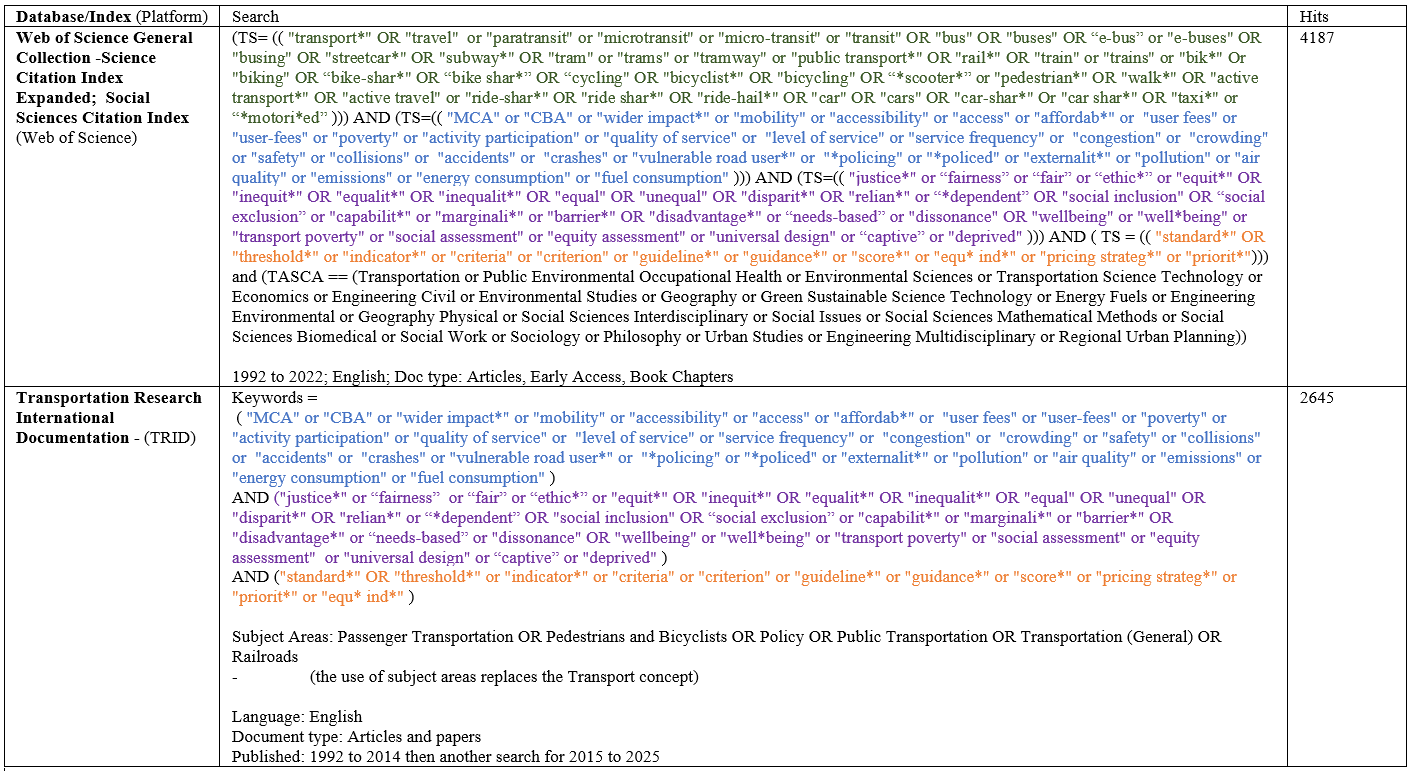
\includegraphics[width=4.7in,height=\textheight]{figures/Search-query.png}

}

\caption{\label{fig-A1}The search query. TS = topic search (keywords,
abstract, title). TASCA = subject categories. Green text area
transportation system related terms, blue text are equity dimension
related terms, purple text are equity/justice conceptualization related
terms, and orange text are standards related terms. Hits corresponds the
number of papers that the search yielded and was retained into the
evidence selection process.}

\end{figure}

Definitions of the population-concept context (PCC) used in the creation
of the inclusion and exclusion criteria for the search strategy.

\begin{itemize}
\tightlist
\item
  \textbf{Population}: the focus of the included studies should be on
  individuals, groups, communities, or entire regional areas that are
  impacted by passenger transportation infrastructure and systems (i.e.,
  all modes and flows) from the perspective of equity (i.e., fair
  distribution, production, and re-production of burdens and benefits).
  This criteria is reflected in the creation of the first set of topic
  search terms that relate to transportation modes (e.g., ``walking'' OR
  ``cycling'' OR ``transit'' - see green text in Figure~\ref{fig-A1} for
  the full list).
\item
  \textbf{Concept}: the included studies should also include equity
  dimensions and conceptualizes equity as discussed in the previous
  section. This inclusion criteria is reflected in the second and third
  set of topic search terms developed in the search strategy. These
  terms relate to types of equity dimensions (e.g., ``accessibility'' OR
  ``mobility'' or ``transport-related air pollution'' - see blue text in
  the Figure~\ref{fig-A1} for the full list) and equity
  conceptualizations (e.g., ``Justice'' OR ``equity'' - see purple text
  in Figure~\ref{fig-A1} for the full list).
\item
  \textbf{Context}: the included studies should also be limited to
  publications that include equity standards. Context can be more
  difficult to explicitly search for with key terms so synonyms for
  `standards' were added to the query as a four set of topic search
  terms (e.g., threshold, indicator, criteria - see orange text in
  Figure~\ref{fig-A1} for full list). Additionally, journal article and
  conference papers, English-language literature from any country, any
  study design (e.g., quantitative, qualitative, or mixed-method
  studies, or conceptual frameworks), and any record published within
  the past 30 years are included (January 1992 to March 2022). The time
  period is selected as the first (to the authors knowledge)
  peer-reviewed article which operationalized equity standards and
  equity conceptualization was published in 1996 (Khisty 1996); we are
  broadening the search by a few years for completeness. English is
  selected as it is the common language spoken across the authorship
  team. Furthermore, papers that explicitly fall within the
  Transportation or related topic/category is included in the query
  (e.g., ``Transportation'', ``Social Sciences'', ``Geography'', ``Civil
  Engineering'', ``Philosophy'' - see the Figure~\ref{fig-A1} for full
  query).
\end{itemize}

The \textbf{exclusion criteria} for the search are papers that are not
within the inclusion criteria. Specifically:

\begin{itemize}
\tightlist
\item
  Literature published before January 1992.
\item
  Papers which do not include transportation equity dimensions.
\item
  Grey as concepts contained within are frequently published in a more
  developed form in journals.
\end{itemize}

\hypertarget{example-of-the-data-extraction-template}{%
\subsection{Example of the data extraction
template:}\label{example-of-the-data-extraction-template}}

\begin{figure}

{\centering 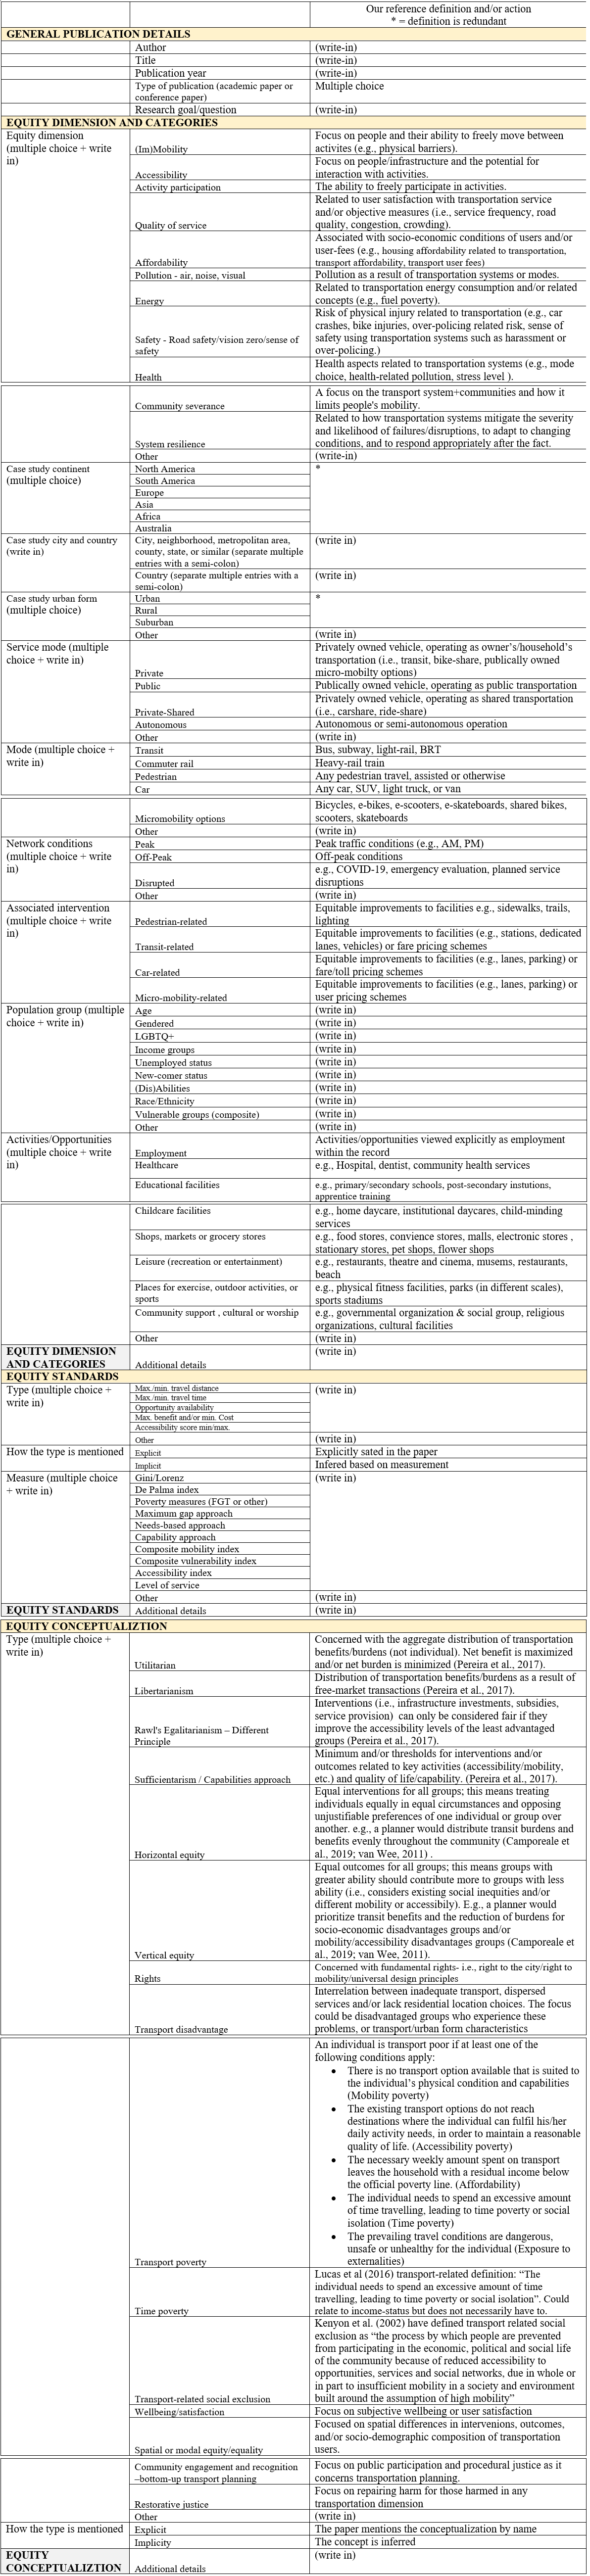
\includegraphics[width=3.97in,height=\textheight]{figures/Data-extract-template.png}

}

\caption{\label{fig-A2}The data extraction template with associated
defintions.}

\end{figure}

\hypertarget{examples-of-papers-summarized-by-element-of-the-analytical-framework}{%
\subsection{Examples of papers summarized by element of the analytical
framework}\label{examples-of-papers-summarized-by-element-of-the-analytical-framework}}

\global\setlength{\Oldarrayrulewidth}{\arrayrulewidth}

\global\setlength{\Oldtabcolsep}{\tabcolsep}

\setlength{\tabcolsep}{0pt}

\renewcommand*{\arraystretch}{1.5}



\providecommand{\ascline}[3]{\noalign{\global\arrayrulewidth #1}\arrayrulecolor[HTML]{#2}\cline{#3}}

\begin{longtable*}[c]{cccc}



\ascline{1.5pt}{666666}{1-4}

\multicolumn{1}{>{}l}{\textcolor[HTML]{000000}{\fontsize{7}{7}\selectfont{Dimension}}} & \multicolumn{1}{>{}l}{\textcolor[HTML]{000000}{\fontsize{7}{7}\selectfont{Continent}}} & \multicolumn{1}{>{}l}{\textcolor[HTML]{000000}{\fontsize{7}{7}\selectfont{Conceptualization}}} & \multicolumn{1}{>{}l}{\textcolor[HTML]{000000}{\fontsize{7}{7}\selectfont{Standard}}} \\

\ascline{1.5pt}{666666}{1-4}\endfirsthead 

\ascline{1.5pt}{666666}{1-4}

\multicolumn{1}{>{}l}{\textcolor[HTML]{000000}{\fontsize{7}{7}\selectfont{Dimension}}} & \multicolumn{1}{>{}l}{\textcolor[HTML]{000000}{\fontsize{7}{7}\selectfont{Continent}}} & \multicolumn{1}{>{}l}{\textcolor[HTML]{000000}{\fontsize{7}{7}\selectfont{Conceptualization}}} & \multicolumn{1}{>{}l}{\textcolor[HTML]{000000}{\fontsize{7}{7}\selectfont{Standard}}} \\

\ascline{1.5pt}{666666}{1-4}\endhead



\multicolumn{1}{>{}l}{} & \multicolumn{1}{>{}l}{\textcolor[HTML]{000000}{\fontsize{7}{7}\selectfont{Where?}}\textcolor[HTML]{000000}{\fontsize{7}{7}\selectfont{\ }}\textcolor[HTML]{000000}{\fontsize{7}{7}\selectfont{(Rivas,}}\textcolor[HTML]{000000}{\fontsize{7}{7}\selectfont{\ }}\textcolor[HTML]{000000}{\fontsize{7}{7}\selectfont{Serebrisky,}}\textcolor[HTML]{000000}{\fontsize{7}{7}\selectfont{\ }}\textcolor[HTML]{000000}{\fontsize{7}{7}\selectfont{and}}\textcolor[HTML]{000000}{\fontsize{7}{7}\selectfont{\ }}\textcolor[HTML]{000000}{\fontsize{7}{7}\selectfont{Suárez-Alemán}}\textcolor[HTML]{000000}{\fontsize{7}{7}\selectfont{\ }}\textcolor[HTML]{000000}{\fontsize{7}{7}\selectfont{2018)}}\textcolor[HTML]{000000}{\fontsize{7}{7}\selectfont{\ }}\textcolor[HTML]{000000}{\fontsize{7}{7}\selectfont{-}}\textcolor[HTML]{000000}{\fontsize{7}{7}\selectfont{\ }}\textcolor[HTML]{000000}{\fontsize{7}{7}\selectfont{South}}\textcolor[HTML]{000000}{\fontsize{7}{7}\selectfont{\ }}\textcolor[HTML]{000000}{\fontsize{7}{7}\selectfont{America}}\textcolor[HTML]{000000}{\fontsize{7}{7}\selectfont{\ }}\textcolor[HTML]{000000}{\fontsize{7}{7}\selectfont{(select}}\textcolor[HTML]{000000}{\fontsize{7}{7}\selectfont{\ }}\textcolor[HTML]{000000}{\fontsize{7}{7}\selectfont{cities)}}} & \multicolumn{1}{>{}l}{\textcolor[HTML]{000000}{\fontsize{7}{7}\selectfont{Analyses}}\textcolor[HTML]{000000}{\fontsize{7}{7}\selectfont{\ }}\textcolor[HTML]{000000}{\fontsize{7}{7}\selectfont{how}}\textcolor[HTML]{000000}{\fontsize{7}{7}\selectfont{\ }}\textcolor[HTML]{000000}{\fontsize{7}{7}\selectfont{affordable}}\textcolor[HTML]{000000}{\fontsize{7}{7}\selectfont{\ }}\textcolor[HTML]{000000}{\fontsize{7}{7}\selectfont{urban}}\textcolor[HTML]{000000}{\fontsize{7}{7}\selectfont{\ }}\textcolor[HTML]{000000}{\fontsize{7}{7}\selectfont{public}}\textcolor[HTML]{000000}{\fontsize{7}{7}\selectfont{\ }}\textcolor[HTML]{000000}{\fontsize{7}{7}\selectfont{transportation}}\textcolor[HTML]{000000}{\fontsize{7}{7}\selectfont{\ }}\textcolor[HTML]{000000}{\fontsize{7}{7}\selectfont{is}}\textcolor[HTML]{000000}{\fontsize{7}{7}\selectfont{\ }}\textcolor[HTML]{000000}{\fontsize{7}{7}\selectfont{in}}\textcolor[HTML]{000000}{\fontsize{7}{7}\selectfont{\ }}\textcolor[HTML]{000000}{\fontsize{7}{7}\selectfont{select}}\textcolor[HTML]{000000}{\fontsize{7}{7}\selectfont{\ }}\textcolor[HTML]{000000}{\fontsize{7}{7}\selectfont{Latin}}\textcolor[HTML]{000000}{\fontsize{7}{7}\selectfont{\ }}\textcolor[HTML]{000000}{\fontsize{7}{7}\selectfont{American}}\textcolor[HTML]{000000}{\fontsize{7}{7}\selectfont{\ }}\textcolor[HTML]{000000}{\fontsize{7}{7}\selectfont{and}}\textcolor[HTML]{000000}{\fontsize{7}{7}\selectfont{\ }}\textcolor[HTML]{000000}{\fontsize{7}{7}\selectfont{Caribbean}}\textcolor[HTML]{000000}{\fontsize{7}{7}\selectfont{\ }}\textcolor[HTML]{000000}{\fontsize{7}{7}\selectfont{countries.}}\textcolor[HTML]{000000}{\fontsize{7}{7}\selectfont{\ }}\textcolor[HTML]{000000}{\fontsize{7}{7}\selectfont{They}}\textcolor[HTML]{000000}{\fontsize{7}{7}\selectfont{\ }}\textcolor[HTML]{000000}{\fontsize{7}{7}\selectfont{look}}\textcolor[HTML]{000000}{\fontsize{7}{7}\selectfont{\ }}\textcolor[HTML]{000000}{\fontsize{7}{7}\selectfont{at}}\textcolor[HTML]{000000}{\fontsize{7}{7}\selectfont{\ }}\textcolor[HTML]{000000}{\fontsize{7}{7}\selectfont{the}}\textcolor[HTML]{000000}{\fontsize{7}{7}\selectfont{\ }}\textcolor[HTML]{000000}{\fontsize{7}{7}\selectfont{estimated}}\textcolor[HTML]{000000}{\fontsize{7}{7}\selectfont{\ }}\textcolor[HTML]{000000}{\fontsize{7}{7}\selectfont{average}}\textcolor[HTML]{000000}{\fontsize{7}{7}\selectfont{\ }}\textcolor[HTML]{000000}{\fontsize{7}{7}\selectfont{monthly}}\textcolor[HTML]{000000}{\fontsize{7}{7}\selectfont{\ }}\textcolor[HTML]{000000}{\fontsize{7}{7}\selectfont{cost}}\textcolor[HTML]{000000}{\fontsize{7}{7}\selectfont{\ }}\textcolor[HTML]{000000}{\fontsize{7}{7}\selectfont{of}}\textcolor[HTML]{000000}{\fontsize{7}{7}\selectfont{\ }}\textcolor[HTML]{000000}{\fontsize{7}{7}\selectfont{transit}}\textcolor[HTML]{000000}{\fontsize{7}{7}\selectfont{\ }}\textcolor[HTML]{000000}{\fontsize{7}{7}\selectfont{trips}}\textcolor[HTML]{000000}{\fontsize{7}{7}\selectfont{\ }}\textcolor[HTML]{000000}{\fontsize{7}{7}\selectfont{and}}\textcolor[HTML]{000000}{\fontsize{7}{7}\selectfont{\ }}\textcolor[HTML]{000000}{\fontsize{7}{7}\selectfont{average}}\textcolor[HTML]{000000}{\fontsize{7}{7}\selectfont{\ }}\textcolor[HTML]{000000}{\fontsize{7}{7}\selectfont{monthly}}\textcolor[HTML]{000000}{\fontsize{7}{7}\selectfont{\ }}\textcolor[HTML]{000000}{\fontsize{7}{7}\selectfont{household}}\textcolor[HTML]{000000}{\fontsize{7}{7}\selectfont{\ }}\textcolor[HTML]{000000}{\fontsize{7}{7}\selectfont{income}}\textcolor[HTML]{000000}{\fontsize{7}{7}\selectfont{\ }}\textcolor[HTML]{000000}{\fontsize{7}{7}\selectfont{and}}\textcolor[HTML]{000000}{\fontsize{7}{7}\selectfont{\ }}\textcolor[HTML]{000000}{\fontsize{7}{7}\selectfont{conceptualize}}\textcolor[HTML]{000000}{\fontsize{7}{7}\selectfont{\ }}\textcolor[HTML]{000000}{\fontsize{7}{7}\selectfont{\textbf{transportation-related}}}\textcolor[HTML]{000000}{\fontsize{7}{7}\selectfont{\ }}\textcolor[HTML]{000000}{\fontsize{7}{7}\selectfont{\textbf{affordability}}}\textcolor[HTML]{000000}{\fontsize{7}{7}\selectfont{,}}\textcolor[HTML]{000000}{\fontsize{7}{7}\selectfont{\ }}\textcolor[HTML]{000000}{\fontsize{7}{7}\selectfont{especially}}\textcolor[HTML]{000000}{\fontsize{7}{7}\selectfont{\ }}\textcolor[HTML]{000000}{\fontsize{7}{7}\selectfont{for}}\textcolor[HTML]{000000}{\fontsize{7}{7}\selectfont{\ }}\textcolor[HTML]{000000}{\fontsize{7}{7}\selectfont{the}}\textcolor[HTML]{000000}{\fontsize{7}{7}\selectfont{\ }}\textcolor[HTML]{000000}{\fontsize{7}{7}\selectfont{most}}\textcolor[HTML]{000000}{\fontsize{7}{7}\selectfont{\ }}\textcolor[HTML]{000000}{\fontsize{7}{7}\selectfont{economically}}\textcolor[HTML]{000000}{\fontsize{7}{7}\selectfont{\ }}\textcolor[HTML]{000000}{\fontsize{7}{7}\selectfont{vulnerable}}\textcolor[HTML]{000000}{\fontsize{7}{7}\selectfont{\ }}\textcolor[HTML]{000000}{\fontsize{7}{7}\selectfont{(}}\textcolor[HTML]{000000}{\fontsize{7}{7}\selectfont{\textbf{vertical}}}\textcolor[HTML]{000000}{\fontsize{7}{7}\selectfont{\textbf{\ }}}\textcolor[HTML]{000000}{\fontsize{7}{7}\selectfont{\textbf{equity}}}\textcolor[HTML]{000000}{\fontsize{7}{7}\selectfont{).}}} & \multicolumn{1}{>{}l}{\textcolor[HTML]{000000}{\fontsize{7}{7}\selectfont{How?:}}\textcolor[HTML]{000000}{\fontsize{7}{7}\selectfont{\ }}\textcolor[HTML]{000000}{\fontsize{7}{7}\selectfont{The}}\textcolor[HTML]{000000}{\fontsize{7}{7}\selectfont{\ }}\textcolor[HTML]{000000}{\fontsize{7}{7}\selectfont{financial}}\textcolor[HTML]{000000}{\fontsize{7}{7}\selectfont{\ }}\textcolor[HTML]{000000}{\fontsize{7}{7}\selectfont{burden}}\textcolor[HTML]{000000}{\fontsize{7}{7}\selectfont{\ }}\textcolor[HTML]{000000}{\fontsize{7}{7}\selectfont{of}}\textcolor[HTML]{000000}{\fontsize{7}{7}\selectfont{\ }}\textcolor[HTML]{000000}{\fontsize{7}{7}\selectfont{a}}\textcolor[HTML]{000000}{\fontsize{7}{7}\selectfont{\ }}\textcolor[HTML]{000000}{\fontsize{7}{7}\selectfont{basket}}\textcolor[HTML]{000000}{\fontsize{7}{7}\selectfont{\ }}\textcolor[HTML]{000000}{\fontsize{7}{7}\selectfont{of}}\textcolor[HTML]{000000}{\fontsize{7}{7}\selectfont{\ }}\textcolor[HTML]{000000}{\fontsize{7}{7}\selectfont{urban}}\textcolor[HTML]{000000}{\fontsize{7}{7}\selectfont{\ }}\textcolor[HTML]{000000}{\fontsize{7}{7}\selectfont{public}}\textcolor[HTML]{000000}{\fontsize{7}{7}\selectfont{\ }}\textcolor[HTML]{000000}{\fontsize{7}{7}\selectfont{transportation}}\textcolor[HTML]{000000}{\fontsize{7}{7}\selectfont{\ }}\textcolor[HTML]{000000}{\fontsize{7}{7}\selectfont{trips}}\textcolor[HTML]{000000}{\fontsize{7}{7}\selectfont{\ }}\textcolor[HTML]{000000}{\fontsize{7}{7}\selectfont{(60}}\textcolor[HTML]{000000}{\fontsize{7}{7}\selectfont{\ }}\textcolor[HTML]{000000}{\fontsize{7}{7}\selectfont{trip}}\textcolor[HTML]{000000}{\fontsize{7}{7}\selectfont{\ }}\textcolor[HTML]{000000}{\fontsize{7}{7}\selectfont{fares,}}\textcolor[HTML]{000000}{\fontsize{7}{7}\selectfont{\ }}\textcolor[HTML]{000000}{\fontsize{7}{7}\selectfont{representing}}\textcolor[HTML]{000000}{\fontsize{7}{7}\selectfont{\ }}\textcolor[HTML]{000000}{\fontsize{7}{7}\selectfont{30}}\textcolor[HTML]{000000}{\fontsize{7}{7}\selectfont{\ }}\textcolor[HTML]{000000}{\fontsize{7}{7}\selectfont{round-trips}}\textcolor[HTML]{000000}{\fontsize{7}{7}\selectfont{\ }}\textcolor[HTML]{000000}{\fontsize{7}{7}\selectfont{per}}\textcolor[HTML]{000000}{\fontsize{7}{7}\selectfont{\ }}\textcolor[HTML]{000000}{\fontsize{7}{7}\selectfont{month)}}\textcolor[HTML]{000000}{\fontsize{7}{7}\selectfont{\ }}\textcolor[HTML]{000000}{\fontsize{7}{7}\selectfont{should}}\textcolor[HTML]{000000}{\fontsize{7}{7}\selectfont{\ }}\textcolor[HTML]{000000}{\fontsize{7}{7}\selectfont{not}}\textcolor[HTML]{000000}{\fontsize{7}{7}\selectfont{\ }}\textcolor[HTML]{000000}{\fontsize{7}{7}\selectfont{exceed}}\textcolor[HTML]{000000}{\fontsize{7}{7}\selectfont{\ }}\textcolor[HTML]{000000}{\fontsize{7}{7}\selectfont{10\%}}\textcolor[HTML]{000000}{\fontsize{7}{7}\selectfont{\ }}\textcolor[HTML]{000000}{\fontsize{7}{7}\selectfont{of}}\textcolor[HTML]{000000}{\fontsize{7}{7}\selectfont{\ }}\textcolor[HTML]{000000}{\fontsize{7}{7}\selectfont{household}}\textcolor[HTML]{000000}{\fontsize{7}{7}\selectfont{\ }}\textcolor[HTML]{000000}{\fontsize{7}{7}\selectfont{monthly}}\textcolor[HTML]{000000}{\fontsize{7}{7}\selectfont{\ }}\textcolor[HTML]{000000}{\fontsize{7}{7}\selectfont{income.}}} \\





\multicolumn{1}{>{}l}{} & \multicolumn{1}{>{}l}{\textcolor[HTML]{000000}{\fontsize{7}{7}\selectfont{Where?:}}\textcolor[HTML]{000000}{\fontsize{7}{7}\selectfont{\ }}\textcolor[HTML]{000000}{\fontsize{7}{7}\selectfont{(Bharathy}}\textcolor[HTML]{000000}{\fontsize{7}{7}\selectfont{\ }}\textcolor[HTML]{000000}{\fontsize{7}{7}\selectfont{and}}\textcolor[HTML]{000000}{\fontsize{7}{7}\selectfont{\ }}\textcolor[HTML]{000000}{\fontsize{7}{7}\selectfont{D’Souza}}\textcolor[HTML]{000000}{\fontsize{7}{7}\selectfont{\ }}\textcolor[HTML]{000000}{\fontsize{7}{7}\selectfont{2018)}}\textcolor[HTML]{000000}{\fontsize{7}{7}\selectfont{\ }}\textcolor[HTML]{000000}{\fontsize{7}{7}\selectfont{-}}\textcolor[HTML]{000000}{\fontsize{7}{7}\selectfont{\ }}\textcolor[HTML]{000000}{\fontsize{7}{7}\selectfont{North}}\textcolor[HTML]{000000}{\fontsize{7}{7}\selectfont{\ }}\textcolor[HTML]{000000}{\fontsize{7}{7}\selectfont{America}}\textcolor[HTML]{000000}{\fontsize{7}{7}\selectfont{\ }}\textcolor[HTML]{000000}{\fontsize{7}{7}\selectfont{(USA}}\textcolor[HTML]{000000}{\fontsize{7}{7}\selectfont{\ }}\textcolor[HTML]{000000}{\fontsize{7}{7}\selectfont{-}}\textcolor[HTML]{000000}{\fontsize{7}{7}\selectfont{\ }}\textcolor[HTML]{000000}{\fontsize{7}{7}\selectfont{National)}}} & \multicolumn{1}{>{}l}{\textcolor[HTML]{000000}{\fontsize{7}{7}\selectfont{This}}\textcolor[HTML]{000000}{\fontsize{7}{7}\selectfont{\ }}\textcolor[HTML]{000000}{\fontsize{7}{7}\selectfont{study}}\textcolor[HTML]{000000}{\fontsize{7}{7}\selectfont{\ }}\textcolor[HTML]{000000}{\fontsize{7}{7}\selectfont{designed}}\textcolor[HTML]{000000}{\fontsize{7}{7}\selectfont{\ }}\textcolor[HTML]{000000}{\fontsize{7}{7}\selectfont{a}}\textcolor[HTML]{000000}{\fontsize{7}{7}\selectfont{\ }}\textcolor[HTML]{000000}{\fontsize{7}{7}\selectfont{web-based}}\textcolor[HTML]{000000}{\fontsize{7}{7}\selectfont{\ }}\textcolor[HTML]{000000}{\fontsize{7}{7}\selectfont{tool}}\textcolor[HTML]{000000}{\fontsize{7}{7}\selectfont{\ }}\textcolor[HTML]{000000}{\fontsize{7}{7}\selectfont{and}}\textcolor[HTML]{000000}{\fontsize{7}{7}\selectfont{\ }}\textcolor[HTML]{000000}{\fontsize{7}{7}\selectfont{took}}\textcolor[HTML]{000000}{\fontsize{7}{7}\selectfont{\ }}\textcolor[HTML]{000000}{\fontsize{7}{7}\selectfont{a}}\textcolor[HTML]{000000}{\fontsize{7}{7}\selectfont{\ }}\textcolor[HTML]{000000}{\fontsize{7}{7}\selectfont{representative}}\textcolor[HTML]{000000}{\fontsize{7}{7}\selectfont{\ }}\textcolor[HTML]{000000}{\fontsize{7}{7}\selectfont{sample}}\textcolor[HTML]{000000}{\fontsize{7}{7}\selectfont{\ }}\textcolor[HTML]{000000}{\fontsize{7}{7}\selectfont{of}}\textcolor[HTML]{000000}{\fontsize{7}{7}\selectfont{\ }}\textcolor[HTML]{000000}{\fontsize{7}{7}\selectfont{wheeled}}\textcolor[HTML]{000000}{\fontsize{7}{7}\selectfont{\ }}\textcolor[HTML]{000000}{\fontsize{7}{7}\selectfont{mobility}}\textcolor[HTML]{000000}{\fontsize{7}{7}\selectfont{\ }}\textcolor[HTML]{000000}{\fontsize{7}{7}\selectfont{device}}\textcolor[HTML]{000000}{\fontsize{7}{7}\selectfont{\ }}\textcolor[HTML]{000000}{\fontsize{7}{7}\selectfont{(WhMD)}}\textcolor[HTML]{000000}{\fontsize{7}{7}\selectfont{\ }}\textcolor[HTML]{000000}{\fontsize{7}{7}\selectfont{users}}\textcolor[HTML]{000000}{\fontsize{7}{7}\selectfont{\ }}\textcolor[HTML]{000000}{\fontsize{7}{7}\selectfont{anthropometry}}\textcolor[HTML]{000000}{\fontsize{7}{7}\selectfont{\ }}\textcolor[HTML]{000000}{\fontsize{7}{7}\selectfont{measurements}}\textcolor[HTML]{000000}{\fontsize{7}{7}\selectfont{\ }}\textcolor[HTML]{000000}{\fontsize{7}{7}\selectfont{to}}\textcolor[HTML]{000000}{\fontsize{7}{7}\selectfont{\ }}\textcolor[HTML]{000000}{\fontsize{7}{7}\selectfont{determine}}\textcolor[HTML]{000000}{\fontsize{7}{7}\selectfont{\ }}\textcolor[HTML]{000000}{\fontsize{7}{7}\selectfont{if}}\textcolor[HTML]{000000}{\fontsize{7}{7}\selectfont{\ }}\textcolor[HTML]{000000}{\fontsize{7}{7}\selectfont{the}}\textcolor[HTML]{000000}{\fontsize{7}{7}\selectfont{\ }}\textcolor[HTML]{000000}{\fontsize{7}{7}\selectfont{minimum}}\textcolor[HTML]{000000}{\fontsize{7}{7}\selectfont{\ }}\textcolor[HTML]{000000}{\fontsize{7}{7}\selectfont{standard}}\textcolor[HTML]{000000}{\fontsize{7}{7}\selectfont{\ }}\textcolor[HTML]{000000}{\fontsize{7}{7}\selectfont{suggested}}\textcolor[HTML]{000000}{\fontsize{7}{7}\selectfont{\ }}\textcolor[HTML]{000000}{\fontsize{7}{7}\selectfont{by}}\textcolor[HTML]{000000}{\fontsize{7}{7}\selectfont{\ }}\textcolor[HTML]{000000}{\fontsize{7}{7}\selectfont{the}}\textcolor[HTML]{000000}{\fontsize{7}{7}\selectfont{\ }}\textcolor[HTML]{000000}{\fontsize{7}{7}\selectfont{ADA}}\textcolor[HTML]{000000}{\fontsize{7}{7}\selectfont{\ }}\textcolor[HTML]{000000}{\fontsize{7}{7}\selectfont{is}}\textcolor[HTML]{000000}{\fontsize{7}{7}\selectfont{\ }}\textcolor[HTML]{000000}{\fontsize{7}{7}\selectfont{sufficient.}}\textcolor[HTML]{000000}{\fontsize{7}{7}\selectfont{\ }}\textcolor[HTML]{000000}{\fontsize{7}{7}\selectfont{We}}\textcolor[HTML]{000000}{\fontsize{7}{7}\selectfont{\ }}\textcolor[HTML]{000000}{\fontsize{7}{7}\selectfont{understand}}\textcolor[HTML]{000000}{\fontsize{7}{7}\selectfont{\ }}\textcolor[HTML]{000000}{\fontsize{7}{7}\selectfont{this}}\textcolor[HTML]{000000}{\fontsize{7}{7}\selectfont{\ }}\textcolor[HTML]{000000}{\fontsize{7}{7}\selectfont{conceptualization}}\textcolor[HTML]{000000}{\fontsize{7}{7}\selectfont{\ }}\textcolor[HTML]{000000}{\fontsize{7}{7}\selectfont{as}}\textcolor[HTML]{000000}{\fontsize{7}{7}\selectfont{\ }}\textcolor[HTML]{000000}{\fontsize{7}{7}\selectfont{a}}\textcolor[HTML]{000000}{\fontsize{7}{7}\selectfont{\ }}\textcolor[HTML]{000000}{\fontsize{7}{7}\selectfont{type}}\textcolor[HTML]{000000}{\fontsize{7}{7}\selectfont{\ }}\textcolor[HTML]{000000}{\fontsize{7}{7}\selectfont{of}}\textcolor[HTML]{000000}{\fontsize{7}{7}\selectfont{\ }}\textcolor[HTML]{000000}{\fontsize{7}{7}\selectfont{\textbf{Rights}}}\textcolor[HTML]{000000}{\fontsize{7}{7}\selectfont{\ }}\textcolor[HTML]{000000}{\fontsize{7}{7}\selectfont{conceptualization}}\textcolor[HTML]{000000}{\fontsize{7}{7}\selectfont{\ }}\textcolor[HTML]{000000}{\fontsize{7}{7}\selectfont{that}}\textcolor[HTML]{000000}{\fontsize{7}{7}\selectfont{\ }}\textcolor[HTML]{000000}{\fontsize{7}{7}\selectfont{WhMD}}\textcolor[HTML]{000000}{\fontsize{7}{7}\selectfont{\ }}\textcolor[HTML]{000000}{\fontsize{7}{7}\selectfont{should}}\textcolor[HTML]{000000}{\fontsize{7}{7}\selectfont{\ }}\textcolor[HTML]{000000}{\fontsize{7}{7}\selectfont{have}}\textcolor[HTML]{000000}{\fontsize{7}{7}\selectfont{\ }}\textcolor[HTML]{000000}{\fontsize{7}{7}\selectfont{minimum}}\textcolor[HTML]{000000}{\fontsize{7}{7}\selectfont{\ }}\textcolor[HTML]{000000}{\fontsize{7}{7}\selectfont{clear}}\textcolor[HTML]{000000}{\fontsize{7}{7}\selectfont{\ }}\textcolor[HTML]{000000}{\fontsize{7}{7}\selectfont{floor}}\textcolor[HTML]{000000}{\fontsize{7}{7}\selectfont{\ }}\textcolor[HTML]{000000}{\fontsize{7}{7}\selectfont{space}}\textcolor[HTML]{000000}{\fontsize{7}{7}\selectfont{\ }}\textcolor[HTML]{000000}{\fontsize{7}{7}\selectfont{(as}}\textcolor[HTML]{000000}{\fontsize{7}{7}\selectfont{\ }}\textcolor[HTML]{000000}{\fontsize{7}{7}\selectfont{described}}\textcolor[HTML]{000000}{\fontsize{7}{7}\selectfont{\ }}\textcolor[HTML]{000000}{\fontsize{7}{7}\selectfont{the}}\textcolor[HTML]{000000}{\fontsize{7}{7}\selectfont{\ }}\textcolor[HTML]{000000}{\fontsize{7}{7}\selectfont{guidelines}}\textcolor[HTML]{000000}{\fontsize{7}{7}\selectfont{\ }}\textcolor[HTML]{000000}{\fontsize{7}{7}\selectfont{in}}\textcolor[HTML]{000000}{\fontsize{7}{7}\selectfont{\ }}\textcolor[HTML]{000000}{\fontsize{7}{7}\selectfont{line}}\textcolor[HTML]{000000}{\fontsize{7}{7}\selectfont{\ }}\textcolor[HTML]{000000}{\fontsize{7}{7}\selectfont{with}}\textcolor[HTML]{000000}{\fontsize{7}{7}\selectfont{\ }}\textcolor[HTML]{000000}{\fontsize{7}{7}\selectfont{the}}\textcolor[HTML]{000000}{\fontsize{7}{7}\selectfont{\ }}\textcolor[HTML]{000000}{\fontsize{7}{7}\selectfont{American}}\textcolor[HTML]{000000}{\fontsize{7}{7}\selectfont{\ }}\textcolor[HTML]{000000}{\fontsize{7}{7}\selectfont{Disabilities}}\textcolor[HTML]{000000}{\fontsize{7}{7}\selectfont{\ }}\textcolor[HTML]{000000}{\fontsize{7}{7}\selectfont{Act)}}\textcolor[HTML]{000000}{\fontsize{7}{7}\selectfont{\ }}\textcolor[HTML]{000000}{\fontsize{7}{7}\selectfont{to}}\textcolor[HTML]{000000}{\fontsize{7}{7}\selectfont{\ }}\textcolor[HTML]{000000}{\fontsize{7}{7}\selectfont{access}}\textcolor[HTML]{000000}{\fontsize{7}{7}\selectfont{\ }}\textcolor[HTML]{000000}{\fontsize{7}{7}\selectfont{bus}}\textcolor[HTML]{000000}{\fontsize{7}{7}\selectfont{\ }}\textcolor[HTML]{000000}{\fontsize{7}{7}\selectfont{shelters,}}\textcolor[HTML]{000000}{\fontsize{7}{7}\selectfont{\ }}\textcolor[HTML]{000000}{\fontsize{7}{7}\selectfont{bus}}\textcolor[HTML]{000000}{\fontsize{7}{7}\selectfont{\ }}\textcolor[HTML]{000000}{\fontsize{7}{7}\selectfont{stop}}\textcolor[HTML]{000000}{\fontsize{7}{7}\selectfont{\ }}\textcolor[HTML]{000000}{\fontsize{7}{7}\selectfont{pads,}}\textcolor[HTML]{000000}{\fontsize{7}{7}\selectfont{\ }}\textcolor[HTML]{000000}{\fontsize{7}{7}\selectfont{and}}\textcolor[HTML]{000000}{\fontsize{7}{7}\selectfont{\ }}\textcolor[HTML]{000000}{\fontsize{7}{7}\selectfont{transit}}\textcolor[HTML]{000000}{\fontsize{7}{7}\selectfont{\ }}\textcolor[HTML]{000000}{\fontsize{7}{7}\selectfont{terminals.}}} & \multicolumn{1}{>{}l}{\textcolor[HTML]{000000}{\fontsize{7}{7}\selectfont{How?:}}\textcolor[HTML]{000000}{\fontsize{7}{7}\selectfont{\ }}\textcolor[HTML]{000000}{\fontsize{7}{7}\selectfont{The}}\textcolor[HTML]{000000}{\fontsize{7}{7}\selectfont{\ }}\textcolor[HTML]{000000}{\fontsize{7}{7}\selectfont{clear}}\textcolor[HTML]{000000}{\fontsize{7}{7}\selectfont{\ }}\textcolor[HTML]{000000}{\fontsize{7}{7}\selectfont{floor}}\textcolor[HTML]{000000}{\fontsize{7}{7}\selectfont{\ }}\textcolor[HTML]{000000}{\fontsize{7}{7}\selectfont{area}}\textcolor[HTML]{000000}{\fontsize{7}{7}\selectfont{\ }}\textcolor[HTML]{000000}{\fontsize{7}{7}\selectfont{for}}\textcolor[HTML]{000000}{\fontsize{7}{7}\selectfont{\ }}\textcolor[HTML]{000000}{\fontsize{7}{7}\selectfont{wheelchairs:}}\textcolor[HTML]{000000}{\fontsize{7}{7}\selectfont{\ }}\textcolor[HTML]{000000}{\fontsize{7}{7}\selectfont{760}}\textcolor[HTML]{000000}{\fontsize{7}{7}\selectfont{\ }}\textcolor[HTML]{000000}{\fontsize{7}{7}\selectfont{mm}}\textcolor[HTML]{000000}{\fontsize{7}{7}\selectfont{\ }}\textcolor[HTML]{000000}{\fontsize{7}{7}\selectfont{(30}}\textcolor[HTML]{000000}{\fontsize{7}{7}\selectfont{\ }}\textcolor[HTML]{000000}{\fontsize{7}{7}\selectfont{in.)}}\textcolor[HTML]{000000}{\fontsize{7}{7}\selectfont{\ }}\textcolor[HTML]{000000}{\fontsize{7}{7}\selectfont{wide}}\textcolor[HTML]{000000}{\fontsize{7}{7}\selectfont{\ }}\textcolor[HTML]{000000}{\fontsize{7}{7}\selectfont{by}}\textcolor[HTML]{000000}{\fontsize{7}{7}\selectfont{\ }}\textcolor[HTML]{000000}{\fontsize{7}{7}\selectfont{1220}}\textcolor[HTML]{000000}{\fontsize{7}{7}\selectfont{\ }}\textcolor[HTML]{000000}{\fontsize{7}{7}\selectfont{mm}}\textcolor[HTML]{000000}{\fontsize{7}{7}\selectfont{\ }}\textcolor[HTML]{000000}{\fontsize{7}{7}\selectfont{(48}}\textcolor[HTML]{000000}{\fontsize{7}{7}\selectfont{\ }}\textcolor[HTML]{000000}{\fontsize{7}{7}\selectfont{in.)}}\textcolor[HTML]{000000}{\fontsize{7}{7}\selectfont{\ }}\textcolor[HTML]{000000}{\fontsize{7}{7}\selectfont{in}}\textcolor[HTML]{000000}{\fontsize{7}{7}\selectfont{\ }}\textcolor[HTML]{000000}{\fontsize{7}{7}\selectfont{length}}\textcolor[HTML]{000000}{\fontsize{7}{7}\selectfont{\ }}\textcolor[HTML]{000000}{\fontsize{7}{7}\selectfont{as}}\textcolor[HTML]{000000}{\fontsize{7}{7}\selectfont{\ }}\textcolor[HTML]{000000}{\fontsize{7}{7}\selectfont{described}}\textcolor[HTML]{000000}{\fontsize{7}{7}\selectfont{\ }}\textcolor[HTML]{000000}{\fontsize{7}{7}\selectfont{by}}\textcolor[HTML]{000000}{\fontsize{7}{7}\selectfont{\ }}\textcolor[HTML]{000000}{\fontsize{7}{7}\selectfont{the}}\textcolor[HTML]{000000}{\fontsize{7}{7}\selectfont{\ }}\textcolor[HTML]{000000}{\fontsize{7}{7}\selectfont{ADA}}\textcolor[HTML]{000000}{\fontsize{7}{7}\selectfont{\ }}\textcolor[HTML]{000000}{\fontsize{7}{7}\selectfont{standards.}}\textcolor[HTML]{000000}{\fontsize{7}{7}\selectfont{\ }}\textcolor[HTML]{000000}{\fontsize{7}{7}\selectfont{Of}}\textcolor[HTML]{000000}{\fontsize{7}{7}\selectfont{\ }}\textcolor[HTML]{000000}{\fontsize{7}{7}\selectfont{note,}}\textcolor[HTML]{000000}{\fontsize{7}{7}\selectfont{\ }}\textcolor[HTML]{000000}{\fontsize{7}{7}\selectfont{this}}\textcolor[HTML]{000000}{\fontsize{7}{7}\selectfont{\ }}\textcolor[HTML]{000000}{\fontsize{7}{7}\selectfont{minimum}}\textcolor[HTML]{000000}{\fontsize{7}{7}\selectfont{\ }}\textcolor[HTML]{000000}{\fontsize{7}{7}\selectfont{clear}}\textcolor[HTML]{000000}{\fontsize{7}{7}\selectfont{\ }}\textcolor[HTML]{000000}{\fontsize{7}{7}\selectfont{floor}}\textcolor[HTML]{000000}{\fontsize{7}{7}\selectfont{\ }}\textcolor[HTML]{000000}{\fontsize{7}{7}\selectfont{area}}\textcolor[HTML]{000000}{\fontsize{7}{7}\selectfont{\ }}\textcolor[HTML]{000000}{\fontsize{7}{7}\selectfont{is}}\textcolor[HTML]{000000}{\fontsize{7}{7}\selectfont{\ }}\textcolor[HTML]{000000}{\fontsize{7}{7}\selectfont{insufficient}}\textcolor[HTML]{000000}{\fontsize{7}{7}\selectfont{\ }}\textcolor[HTML]{000000}{\fontsize{7}{7}\selectfont{for}}\textcolor[HTML]{000000}{\fontsize{7}{7}\selectfont{\ }}\textcolor[HTML]{000000}{\fontsize{7}{7}\selectfont{a}}\textcolor[HTML]{000000}{\fontsize{7}{7}\selectfont{\ }}\textcolor[HTML]{000000}{\fontsize{7}{7}\selectfont{variety}}\textcolor[HTML]{000000}{\fontsize{7}{7}\selectfont{\ }}\textcolor[HTML]{000000}{\fontsize{7}{7}\selectfont{of}}\textcolor[HTML]{000000}{\fontsize{7}{7}\selectfont{\ }}\textcolor[HTML]{000000}{\fontsize{7}{7}\selectfont{the}}\textcolor[HTML]{000000}{\fontsize{7}{7}\selectfont{\ }}\textcolor[HTML]{000000}{\fontsize{7}{7}\selectfont{WhMD}}\textcolor[HTML]{000000}{\fontsize{7}{7}\selectfont{\ }}\textcolor[HTML]{000000}{\fontsize{7}{7}\selectfont{users.}}} \\





\multicolumn{1}{>{}l}{} & \multicolumn{1}{>{}l}{\textcolor[HTML]{000000}{\fontsize{7}{7}\selectfont{(Ryan}}\textcolor[HTML]{000000}{\fontsize{7}{7}\selectfont{\ }}\textcolor[HTML]{000000}{\fontsize{7}{7}\selectfont{and}}\textcolor[HTML]{000000}{\fontsize{7}{7}\selectfont{\ }}\textcolor[HTML]{000000}{\fontsize{7}{7}\selectfont{Pereira}}\textcolor[HTML]{000000}{\fontsize{7}{7}\selectfont{\ }}\textcolor[HTML]{000000}{\fontsize{7}{7}\selectfont{2021)}}\textcolor[HTML]{000000}{\fontsize{7}{7}\selectfont{\ }}\textcolor[HTML]{000000}{\fontsize{7}{7}\selectfont{-}}\textcolor[HTML]{000000}{\fontsize{7}{7}\selectfont{\ }}\textcolor[HTML]{000000}{\fontsize{7}{7}\selectfont{Europe}}\textcolor[HTML]{000000}{\fontsize{7}{7}\selectfont{\ }}\textcolor[HTML]{000000}{\fontsize{7}{7}\selectfont{(Stockholm,}}\textcolor[HTML]{000000}{\fontsize{7}{7}\selectfont{\ }}\textcolor[HTML]{000000}{\fontsize{7}{7}\selectfont{Gothenburg}}\textcolor[HTML]{000000}{\fontsize{7}{7}\selectfont{\ }}\textcolor[HTML]{000000}{\fontsize{7}{7}\selectfont{and}}\textcolor[HTML]{000000}{\fontsize{7}{7}\selectfont{\ }}\textcolor[HTML]{000000}{\fontsize{7}{7}\selectfont{Malmo}}\textcolor[HTML]{000000}{\fontsize{7}{7}\selectfont{\ }}\textcolor[HTML]{000000}{\fontsize{7}{7}\selectfont{cities}}\textcolor[HTML]{000000}{\fontsize{7}{7}\selectfont{\ }}\textcolor[HTML]{000000}{\fontsize{7}{7}\selectfont{in}}\textcolor[HTML]{000000}{\fontsize{7}{7}\selectfont{\ }}\textcolor[HTML]{000000}{\fontsize{7}{7}\selectfont{Sweden)}}} & \multicolumn{1}{>{}l}{\textcolor[HTML]{000000}{\fontsize{7}{7}\selectfont{Investigates}}\textcolor[HTML]{000000}{\fontsize{7}{7}\selectfont{\ }}\textcolor[HTML]{000000}{\fontsize{7}{7}\selectfont{what}}\textcolor[HTML]{000000}{\fontsize{7}{7}\selectfont{\ }}\textcolor[HTML]{000000}{\fontsize{7}{7}\selectfont{the}}\textcolor[HTML]{000000}{\fontsize{7}{7}\selectfont{\ }}\textcolor[HTML]{000000}{\fontsize{7}{7}\selectfont{literature}}\textcolor[HTML]{000000}{\fontsize{7}{7}\selectfont{\ }}\textcolor[HTML]{000000}{\fontsize{7}{7}\selectfont{and}}\textcolor[HTML]{000000}{\fontsize{7}{7}\selectfont{\ }}\textcolor[HTML]{000000}{\fontsize{7}{7}\selectfont{planning}}\textcolor[HTML]{000000}{\fontsize{7}{7}\selectfont{\ }}\textcolor[HTML]{000000}{\fontsize{7}{7}\selectfont{process}}\textcolor[HTML]{000000}{\fontsize{7}{7}\selectfont{\ }}\textcolor[HTML]{000000}{\fontsize{7}{7}\selectfont{is}}\textcolor[HTML]{000000}{\fontsize{7}{7}\selectfont{\ }}\textcolor[HTML]{000000}{\fontsize{7}{7}\selectfont{missing}}\textcolor[HTML]{000000}{\fontsize{7}{7}\selectfont{\ }}\textcolor[HTML]{000000}{\fontsize{7}{7}\selectfont{when}}\textcolor[HTML]{000000}{\fontsize{7}{7}\selectfont{\ }}\textcolor[HTML]{000000}{\fontsize{7}{7}\selectfont{we}}\textcolor[HTML]{000000}{\fontsize{7}{7}\selectfont{\ }}\textcolor[HTML]{000000}{\fontsize{7}{7}\selectfont{measure}}\textcolor[HTML]{000000}{\fontsize{7}{7}\selectfont{\ }}\textcolor[HTML]{000000}{\fontsize{7}{7}\selectfont{accessibility}}\textcolor[HTML]{000000}{\fontsize{7}{7}\selectfont{\ }}\textcolor[HTML]{000000}{\fontsize{7}{7}\selectfont{by}}\textcolor[HTML]{000000}{\fontsize{7}{7}\selectfont{\ }}\textcolor[HTML]{000000}{\fontsize{7}{7}\selectfont{comparing}}\textcolor[HTML]{000000}{\fontsize{7}{7}\selectfont{\ }}\textcolor[HTML]{000000}{\fontsize{7}{7}\selectfont{objective}}\textcolor[HTML]{000000}{\fontsize{7}{7}\selectfont{\ }}\textcolor[HTML]{000000}{\fontsize{7}{7}\selectfont{and}}\textcolor[HTML]{000000}{\fontsize{7}{7}\selectfont{\ }}\textcolor[HTML]{000000}{\fontsize{7}{7}\selectfont{self-reported}}\textcolor[HTML]{000000}{\fontsize{7}{7}\selectfont{\ }}\textcolor[HTML]{000000}{\fontsize{7}{7}\selectfont{accounts}}\textcolor[HTML]{000000}{\fontsize{7}{7}\selectfont{\ }}\textcolor[HTML]{000000}{\fontsize{7}{7}\selectfont{of}}\textcolor[HTML]{000000}{\fontsize{7}{7}\selectfont{\ }}\textcolor[HTML]{000000}{\fontsize{7}{7}\selectfont{accessibility}}\textcolor[HTML]{000000}{\fontsize{7}{7}\selectfont{\ }}\textcolor[HTML]{000000}{\fontsize{7}{7}\selectfont{among}}\textcolor[HTML]{000000}{\fontsize{7}{7}\selectfont{\ }}\textcolor[HTML]{000000}{\fontsize{7}{7}\selectfont{older}}\textcolor[HTML]{000000}{\fontsize{7}{7}\selectfont{\ }}\textcolor[HTML]{000000}{\fontsize{7}{7}\selectfont{people.}}\textcolor[HTML]{000000}{\fontsize{7}{7}\selectfont{\ }}\textcolor[HTML]{000000}{\fontsize{7}{7}\selectfont{This}}\textcolor[HTML]{000000}{\fontsize{7}{7}\selectfont{\ }}\textcolor[HTML]{000000}{\fontsize{7}{7}\selectfont{paper}}\textcolor[HTML]{000000}{\fontsize{7}{7}\selectfont{\ }}\textcolor[HTML]{000000}{\fontsize{7}{7}\selectfont{conceptualizes}}\textcolor[HTML]{000000}{\fontsize{7}{7}\selectfont{\ }}\textcolor[HTML]{000000}{\fontsize{7}{7}\selectfont{accessibility}}\textcolor[HTML]{000000}{\fontsize{7}{7}\selectfont{\ }}\textcolor[HTML]{000000}{\fontsize{7}{7}\selectfont{as}}\textcolor[HTML]{000000}{\fontsize{7}{7}\selectfont{\ }}\textcolor[HTML]{000000}{\fontsize{7}{7}\selectfont{from}}\textcolor[HTML]{000000}{\fontsize{7}{7}\selectfont{\ }}\textcolor[HTML]{000000}{\fontsize{7}{7}\selectfont{the}}\textcolor[HTML]{000000}{\fontsize{7}{7}\selectfont{\ }}\textcolor[HTML]{000000}{\fontsize{7}{7}\selectfont{position}}\textcolor[HTML]{000000}{\fontsize{7}{7}\selectfont{\ }}\textcolor[HTML]{000000}{\fontsize{7}{7}\selectfont{of}}\textcolor[HTML]{000000}{\fontsize{7}{7}\selectfont{\ }}\textcolor[HTML]{000000}{\fontsize{7}{7}\selectfont{the}}\textcolor[HTML]{000000}{\fontsize{7}{7}\selectfont{\ }}\textcolor[HTML]{000000}{\fontsize{7}{7}\selectfont{\textbf{capabilities}}}\textcolor[HTML]{000000}{\fontsize{7}{7}\selectfont{\textbf{\ }}}\textcolor[HTML]{000000}{\fontsize{7}{7}\selectfont{\textbf{approach}}}\textcolor[HTML]{000000}{\fontsize{7}{7}\selectfont{\ }}\textcolor[HTML]{000000}{\fontsize{7}{7}\selectfont{and}}\textcolor[HTML]{000000}{\fontsize{7}{7}\selectfont{\ }}\textcolor[HTML]{000000}{\fontsize{7}{7}\selectfont{\textbf{vertical}}}\textcolor[HTML]{000000}{\fontsize{7}{7}\selectfont{\textbf{\ }}}\textcolor[HTML]{000000}{\fontsize{7}{7}\selectfont{\textbf{equity}}}\textcolor[HTML]{000000}{\fontsize{7}{7}\selectfont{\ }}\textcolor[HTML]{000000}{\fontsize{7}{7}\selectfont{(particularly}}\textcolor[HTML]{000000}{\fontsize{7}{7}\selectfont{\ }}\textcolor[HTML]{000000}{\fontsize{7}{7}\selectfont{acknowledging}}\textcolor[HTML]{000000}{\fontsize{7}{7}\selectfont{\ }}\textcolor[HTML]{000000}{\fontsize{7}{7}\selectfont{that}}\textcolor[HTML]{000000}{\fontsize{7}{7}\selectfont{\ }}\textcolor[HTML]{000000}{\fontsize{7}{7}\selectfont{older}}\textcolor[HTML]{000000}{\fontsize{7}{7}\selectfont{\ }}\textcolor[HTML]{000000}{\fontsize{7}{7}\selectfont{people}}\textcolor[HTML]{000000}{\fontsize{7}{7}\selectfont{\ }}\textcolor[HTML]{000000}{\fontsize{7}{7}\selectfont{have}}\textcolor[HTML]{000000}{\fontsize{7}{7}\selectfont{\ }}\textcolor[HTML]{000000}{\fontsize{7}{7}\selectfont{capabilities}}\textcolor[HTML]{000000}{\fontsize{7}{7}\selectfont{\ }}\textcolor[HTML]{000000}{\fontsize{7}{7}\selectfont{that}}\textcolor[HTML]{000000}{\fontsize{7}{7}\selectfont{\ }}\textcolor[HTML]{000000}{\fontsize{7}{7}\selectfont{differ}}\textcolor[HTML]{000000}{\fontsize{7}{7}\selectfont{\ }}\textcolor[HTML]{000000}{\fontsize{7}{7}\selectfont{from}}\textcolor[HTML]{000000}{\fontsize{7}{7}\selectfont{\ }}\textcolor[HTML]{000000}{\fontsize{7}{7}\selectfont{the}}\textcolor[HTML]{000000}{\fontsize{7}{7}\selectfont{\ }}\textcolor[HTML]{000000}{\fontsize{7}{7}\selectfont{general}}\textcolor[HTML]{000000}{\fontsize{7}{7}\selectfont{\ }}\textcolor[HTML]{000000}{\fontsize{7}{7}\selectfont{population).}}} & \multicolumn{1}{>{}l}{\textcolor[HTML]{000000}{\fontsize{7}{7}\selectfont{How?:}}\textcolor[HTML]{000000}{\fontsize{7}{7}\selectfont{\ }}\textcolor[HTML]{000000}{\fontsize{7}{7}\selectfont{Specifically}}\textcolor[HTML]{000000}{\fontsize{7}{7}\selectfont{\ }}\textcolor[HTML]{000000}{\fontsize{7}{7}\selectfont{for}}\textcolor[HTML]{000000}{\fontsize{7}{7}\selectfont{\ }}\textcolor[HTML]{000000}{\fontsize{7}{7}\selectfont{older}}\textcolor[HTML]{000000}{\fontsize{7}{7}\selectfont{\ }}\textcolor[HTML]{000000}{\fontsize{7}{7}\selectfont{populations}}\textcolor[HTML]{000000}{\fontsize{7}{7}\selectfont{\ }}\textcolor[HTML]{000000}{\fontsize{7}{7}\selectfont{(aged}}\textcolor[HTML]{000000}{\fontsize{7}{7}\selectfont{\ }}\textcolor[HTML]{000000}{\fontsize{7}{7}\selectfont{65+),}}\textcolor[HTML]{000000}{\fontsize{7}{7}\selectfont{\ }}\textcolor[HTML]{000000}{\fontsize{7}{7}\selectfont{the}}\textcolor[HTML]{000000}{\fontsize{7}{7}\selectfont{\ }}\textcolor[HTML]{000000}{\fontsize{7}{7}\selectfont{following}}\textcolor[HTML]{000000}{\fontsize{7}{7}\selectfont{\ }}\textcolor[HTML]{000000}{\fontsize{7}{7}\selectfont{travel}}\textcolor[HTML]{000000}{\fontsize{7}{7}\selectfont{\ }}\textcolor[HTML]{000000}{\fontsize{7}{7}\selectfont{distances}}\textcolor[HTML]{000000}{\fontsize{7}{7}\selectfont{\ }}\textcolor[HTML]{000000}{\fontsize{7}{7}\selectfont{are}}\textcolor[HTML]{000000}{\fontsize{7}{7}\selectfont{\ }}\textcolor[HTML]{000000}{\fontsize{7}{7}\selectfont{suggested}}\textcolor[HTML]{000000}{\fontsize{7}{7}\selectfont{\ }}\textcolor[HTML]{000000}{\fontsize{7}{7}\selectfont{as}}\textcolor[HTML]{000000}{\fontsize{7}{7}\selectfont{\ }}\textcolor[HTML]{000000}{\fontsize{7}{7}\selectfont{equitable}}\textcolor[HTML]{000000}{\fontsize{7}{7}\selectfont{\ }}\textcolor[HTML]{000000}{\fontsize{7}{7}\selectfont{trip}}\textcolor[HTML]{000000}{\fontsize{7}{7}\selectfont{\ }}\textcolor[HTML]{000000}{\fontsize{7}{7}\selectfont{lengths}}\textcolor[HTML]{000000}{\fontsize{7}{7}\selectfont{\ }}\textcolor[HTML]{000000}{\fontsize{7}{7}\selectfont{to}}\textcolor[HTML]{000000}{\fontsize{7}{7}\selectfont{\ }}\textcolor[HTML]{000000}{\fontsize{7}{7}\selectfont{grocery}}\textcolor[HTML]{000000}{\fontsize{7}{7}\selectfont{\ }}\textcolor[HTML]{000000}{\fontsize{7}{7}\selectfont{stores}}\textcolor[HTML]{000000}{\fontsize{7}{7}\selectfont{\ }}\textcolor[HTML]{000000}{\fontsize{7}{7}\selectfont{per}}\textcolor[HTML]{000000}{\fontsize{7}{7}\selectfont{\ }}\textcolor[HTML]{000000}{\fontsize{7}{7}\selectfont{mode:}}\textcolor[HTML]{000000}{\fontsize{7}{7}\selectfont{\ }}\textcolor[HTML]{000000}{\fontsize{7}{7}\selectfont{Walking:}}\textcolor[HTML]{000000}{\fontsize{7}{7}\selectfont{\ }}\textcolor[HTML]{000000}{\fontsize{7}{7}\selectfont{less}}\textcolor[HTML]{000000}{\fontsize{7}{7}\selectfont{\ }}\textcolor[HTML]{000000}{\fontsize{7}{7}\selectfont{than}}\textcolor[HTML]{000000}{\fontsize{7}{7}\selectfont{\ }}\textcolor[HTML]{000000}{\fontsize{7}{7}\selectfont{or}}\textcolor[HTML]{000000}{\fontsize{7}{7}\selectfont{\ }}\textcolor[HTML]{000000}{\fontsize{7}{7}\selectfont{equal}}\textcolor[HTML]{000000}{\fontsize{7}{7}\selectfont{\ }}\textcolor[HTML]{000000}{\fontsize{7}{7}\selectfont{to}}\textcolor[HTML]{000000}{\fontsize{7}{7}\selectfont{\ }}\textcolor[HTML]{000000}{\fontsize{7}{7}\selectfont{1500m,}}\textcolor[HTML]{000000}{\fontsize{7}{7}\selectfont{\ }}\textcolor[HTML]{000000}{\fontsize{7}{7}\selectfont{Combined}}\textcolor[HTML]{000000}{\fontsize{7}{7}\selectfont{\ }}\textcolor[HTML]{000000}{\fontsize{7}{7}\selectfont{public}}\textcolor[HTML]{000000}{\fontsize{7}{7}\selectfont{\ }}\textcolor[HTML]{000000}{\fontsize{7}{7}\selectfont{transit}}\textcolor[HTML]{000000}{\fontsize{7}{7}\selectfont{\ }}\textcolor[HTML]{000000}{\fontsize{7}{7}\selectfont{and}}\textcolor[HTML]{000000}{\fontsize{7}{7}\selectfont{\ }}\textcolor[HTML]{000000}{\fontsize{7}{7}\selectfont{walking}}\textcolor[HTML]{000000}{\fontsize{7}{7}\selectfont{\ }}\textcolor[HTML]{000000}{\fontsize{7}{7}\selectfont{(less}}\textcolor[HTML]{000000}{\fontsize{7}{7}\selectfont{\ }}\textcolor[HTML]{000000}{\fontsize{7}{7}\selectfont{than}}\textcolor[HTML]{000000}{\fontsize{7}{7}\selectfont{\ }}\textcolor[HTML]{000000}{\fontsize{7}{7}\selectfont{or}}\textcolor[HTML]{000000}{\fontsize{7}{7}\selectfont{\ }}\textcolor[HTML]{000000}{\fontsize{7}{7}\selectfont{equal}}\textcolor[HTML]{000000}{\fontsize{7}{7}\selectfont{\ }}\textcolor[HTML]{000000}{\fontsize{7}{7}\selectfont{to}}\textcolor[HTML]{000000}{\fontsize{7}{7}\selectfont{\ }}\textcolor[HTML]{000000}{\fontsize{7}{7}\selectfont{1000m}}\textcolor[HTML]{000000}{\fontsize{7}{7}\selectfont{\ }}\textcolor[HTML]{000000}{\fontsize{7}{7}\selectfont{(walking}}\textcolor[HTML]{000000}{\fontsize{7}{7}\selectfont{\ }}\textcolor[HTML]{000000}{\fontsize{7}{7}\selectfont{element)),}}\textcolor[HTML]{000000}{\fontsize{7}{7}\selectfont{\ }}\textcolor[HTML]{000000}{\fontsize{7}{7}\selectfont{Combined}}\textcolor[HTML]{000000}{\fontsize{7}{7}\selectfont{\ }}\textcolor[HTML]{000000}{\fontsize{7}{7}\selectfont{car}}\textcolor[HTML]{000000}{\fontsize{7}{7}\selectfont{\ }}\textcolor[HTML]{000000}{\fontsize{7}{7}\selectfont{and}}\textcolor[HTML]{000000}{\fontsize{7}{7}\selectfont{\ }}\textcolor[HTML]{000000}{\fontsize{7}{7}\selectfont{walking:}}\textcolor[HTML]{000000}{\fontsize{7}{7}\selectfont{\ }}\textcolor[HTML]{000000}{\fontsize{7}{7}\selectfont{less}}\textcolor[HTML]{000000}{\fontsize{7}{7}\selectfont{\ }}\textcolor[HTML]{000000}{\fontsize{7}{7}\selectfont{than}}\textcolor[HTML]{000000}{\fontsize{7}{7}\selectfont{\ }}\textcolor[HTML]{000000}{\fontsize{7}{7}\selectfont{or}}\textcolor[HTML]{000000}{\fontsize{7}{7}\selectfont{\ }}\textcolor[HTML]{000000}{\fontsize{7}{7}\selectfont{equal}}\textcolor[HTML]{000000}{\fontsize{7}{7}\selectfont{\ }}\textcolor[HTML]{000000}{\fontsize{7}{7}\selectfont{to}}\textcolor[HTML]{000000}{\fontsize{7}{7}\selectfont{\ }}\textcolor[HTML]{000000}{\fontsize{7}{7}\selectfont{1000m}}\textcolor[HTML]{000000}{\fontsize{7}{7}\selectfont{\ }}\textcolor[HTML]{000000}{\fontsize{7}{7}\selectfont{less}}\textcolor[HTML]{000000}{\fontsize{7}{7}\selectfont{\ }}\textcolor[HTML]{000000}{\fontsize{7}{7}\selectfont{than}}\textcolor[HTML]{000000}{\fontsize{7}{7}\selectfont{\ }}\textcolor[HTML]{000000}{\fontsize{7}{7}\selectfont{or}}\textcolor[HTML]{000000}{\fontsize{7}{7}\selectfont{\ }}\textcolor[HTML]{000000}{\fontsize{7}{7}\selectfont{equal}}\textcolor[HTML]{000000}{\fontsize{7}{7}\selectfont{\ }}\textcolor[HTML]{000000}{\fontsize{7}{7}\selectfont{to}}\textcolor[HTML]{000000}{\fontsize{7}{7}\selectfont{\ }}\textcolor[HTML]{000000}{\fontsize{7}{7}\selectfont{1000m}}\textcolor[HTML]{000000}{\fontsize{7}{7}\selectfont{\ }}\textcolor[HTML]{000000}{\fontsize{7}{7}\selectfont{(walking}}\textcolor[HTML]{000000}{\fontsize{7}{7}\selectfont{\ }}\textcolor[HTML]{000000}{\fontsize{7}{7}\selectfont{element)),}}\textcolor[HTML]{000000}{\fontsize{7}{7}\selectfont{\ }}\textcolor[HTML]{000000}{\fontsize{7}{7}\selectfont{Bicycle:}}\textcolor[HTML]{000000}{\fontsize{7}{7}\selectfont{\ }}\textcolor[HTML]{000000}{\fontsize{7}{7}\selectfont{less}}\textcolor[HTML]{000000}{\fontsize{7}{7}\selectfont{\ }}\textcolor[HTML]{000000}{\fontsize{7}{7}\selectfont{than}}\textcolor[HTML]{000000}{\fontsize{7}{7}\selectfont{\ }}\textcolor[HTML]{000000}{\fontsize{7}{7}\selectfont{or}}\textcolor[HTML]{000000}{\fontsize{7}{7}\selectfont{\ }}\textcolor[HTML]{000000}{\fontsize{7}{7}\selectfont{equal}}\textcolor[HTML]{000000}{\fontsize{7}{7}\selectfont{\ }}\textcolor[HTML]{000000}{\fontsize{7}{7}\selectfont{to}}\textcolor[HTML]{000000}{\fontsize{7}{7}\selectfont{\ }}\textcolor[HTML]{000000}{\fontsize{7}{7}\selectfont{3000m}}\textcolor[HTML]{000000}{\fontsize{7}{7}\selectfont{\ }}\textcolor[HTML]{000000}{\fontsize{7}{7}\selectfont{in}}\textcolor[HTML]{000000}{\fontsize{7}{7}\selectfont{\ }}\textcolor[HTML]{000000}{\fontsize{7}{7}\selectfont{addition}}\textcolor[HTML]{000000}{\fontsize{7}{7}\selectfont{\ }}\textcolor[HTML]{000000}{\fontsize{7}{7}\selectfont{to}}\textcolor[HTML]{000000}{\fontsize{7}{7}\selectfont{\ }}\textcolor[HTML]{000000}{\fontsize{7}{7}\selectfont{travel}}\textcolor[HTML]{000000}{\fontsize{7}{7}\selectfont{\ }}\textcolor[HTML]{000000}{\fontsize{7}{7}\selectfont{time}}\textcolor[HTML]{000000}{\fontsize{7}{7}\selectfont{\ }}\textcolor[HTML]{000000}{\fontsize{7}{7}\selectfont{threshold}}\textcolor[HTML]{000000}{\fontsize{7}{7}\selectfont{\ }}\textcolor[HTML]{000000}{\fontsize{7}{7}\selectfont{of}}\textcolor[HTML]{000000}{\fontsize{7}{7}\selectfont{\ }}\textcolor[HTML]{000000}{\fontsize{7}{7}\selectfont{less}}\textcolor[HTML]{000000}{\fontsize{7}{7}\selectfont{\ }}\textcolor[HTML]{000000}{\fontsize{7}{7}\selectfont{than}}\textcolor[HTML]{000000}{\fontsize{7}{7}\selectfont{\ }}\textcolor[HTML]{000000}{\fontsize{7}{7}\selectfont{15}}\textcolor[HTML]{000000}{\fontsize{7}{7}\selectfont{\ }}\textcolor[HTML]{000000}{\fontsize{7}{7}\selectfont{mins.}}} \\





\multicolumn{1}{>{}l}{} & \multicolumn{1}{>{}l}{\textcolor[HTML]{000000}{\fontsize{7}{7}\selectfont{Where?:}}\textcolor[HTML]{000000}{\fontsize{7}{7}\selectfont{\ }}\textcolor[HTML]{000000}{\fontsize{7}{7}\selectfont{(Wismadi}}\textcolor[HTML]{000000}{\fontsize{7}{7}\selectfont{\ }}\textcolor[HTML]{000000}{\fontsize{7}{7}\selectfont{et}}\textcolor[HTML]{000000}{\fontsize{7}{7}\selectfont{\ }}\textcolor[HTML]{000000}{\fontsize{7}{7}\selectfont{al.}}\textcolor[HTML]{000000}{\fontsize{7}{7}\selectfont{\ }}\textcolor[HTML]{000000}{\fontsize{7}{7}\selectfont{2014)}}\textcolor[HTML]{000000}{\fontsize{7}{7}\selectfont{\ }}\textcolor[HTML]{000000}{\fontsize{7}{7}\selectfont{-}}\textcolor[HTML]{000000}{\fontsize{7}{7}\selectfont{\ }}\textcolor[HTML]{000000}{\fontsize{7}{7}\selectfont{Asia}}\textcolor[HTML]{000000}{\fontsize{7}{7}\selectfont{\ }}\textcolor[HTML]{000000}{\fontsize{7}{7}\selectfont{(Yogyakarta,}}\textcolor[HTML]{000000}{\fontsize{7}{7}\selectfont{\ }}\textcolor[HTML]{000000}{\fontsize{7}{7}\selectfont{Indonesia)}}} & \multicolumn{1}{>{}l}{\textcolor[HTML]{000000}{\fontsize{7}{7}\selectfont{Explores}}\textcolor[HTML]{000000}{\fontsize{7}{7}\selectfont{\ }}\textcolor[HTML]{000000}{\fontsize{7}{7}\selectfont{the}}\textcolor[HTML]{000000}{\fontsize{7}{7}\selectfont{\ }}\textcolor[HTML]{000000}{\fontsize{7}{7}\selectfont{equitable}}\textcolor[HTML]{000000}{\fontsize{7}{7}\selectfont{\ }}\textcolor[HTML]{000000}{\fontsize{7}{7}\selectfont{provision}}\textcolor[HTML]{000000}{\fontsize{7}{7}\selectfont{\ }}\textcolor[HTML]{000000}{\fontsize{7}{7}\selectfont{of}}\textcolor[HTML]{000000}{\fontsize{7}{7}\selectfont{\ }}\textcolor[HTML]{000000}{\fontsize{7}{7}\selectfont{transport}}\textcolor[HTML]{000000}{\fontsize{7}{7}\selectfont{\ }}\textcolor[HTML]{000000}{\fontsize{7}{7}\selectfont{infrastructure}}\textcolor[HTML]{000000}{\fontsize{7}{7}\selectfont{\ }}\textcolor[HTML]{000000}{\fontsize{7}{7}\selectfont{provision:}}\textcolor[HTML]{000000}{\fontsize{7}{7}\selectfont{\ }}\textcolor[HTML]{000000}{\fontsize{7}{7}\selectfont{an}}\textcolor[HTML]{000000}{\fontsize{7}{7}\selectfont{\ }}\textcolor[HTML]{000000}{\fontsize{7}{7}\selectfont{application}}\textcolor[HTML]{000000}{\fontsize{7}{7}\selectfont{\ }}\textcolor[HTML]{000000}{\fontsize{7}{7}\selectfont{of}}\textcolor[HTML]{000000}{\fontsize{7}{7}\selectfont{\ }}\textcolor[HTML]{000000}{\fontsize{7}{7}\selectfont{Sen’s}}\textcolor[HTML]{000000}{\fontsize{7}{7}\selectfont{\ }}\textcolor[HTML]{000000}{\fontsize{7}{7}\selectfont{\textbf{capability}}}\textcolor[HTML]{000000}{\fontsize{7}{7}\selectfont{\textbf{\ }}}\textcolor[HTML]{000000}{\fontsize{7}{7}\selectfont{\textbf{approach}}}\textcolor[HTML]{000000}{\fontsize{7}{7}\selectfont{.}}\textcolor[HTML]{000000}{\fontsize{7}{7}\selectfont{\ }}\textcolor[HTML]{000000}{\fontsize{7}{7}\selectfont{Conceptualizes}}\textcolor[HTML]{000000}{\fontsize{7}{7}\selectfont{\ }}\textcolor[HTML]{000000}{\fontsize{7}{7}\selectfont{equity}}\textcolor[HTML]{000000}{\fontsize{7}{7}\selectfont{\ }}\textcolor[HTML]{000000}{\fontsize{7}{7}\selectfont{through}}\textcolor[HTML]{000000}{\fontsize{7}{7}\selectfont{\ }}\textcolor[HTML]{000000}{\fontsize{7}{7}\selectfont{Sen’s}}\textcolor[HTML]{000000}{\fontsize{7}{7}\selectfont{\ }}\textcolor[HTML]{000000}{\fontsize{7}{7}\selectfont{capability}}\textcolor[HTML]{000000}{\fontsize{7}{7}\selectfont{\ }}\textcolor[HTML]{000000}{\fontsize{7}{7}\selectfont{approach}}\textcolor[HTML]{000000}{\fontsize{7}{7}\selectfont{\ }}\textcolor[HTML]{000000}{\fontsize{7}{7}\selectfont{and}}\textcolor[HTML]{000000}{\fontsize{7}{7}\selectfont{\ }}\textcolor[HTML]{000000}{\fontsize{7}{7}\selectfont{spatial}}\textcolor[HTML]{000000}{\fontsize{7}{7}\selectfont{\ }}\textcolor[HTML]{000000}{\fontsize{7}{7}\selectfont{equity.}}} & \multicolumn{1}{>{}l}{\textcolor[HTML]{000000}{\fontsize{7}{7}\selectfont{How?:}}\textcolor[HTML]{000000}{\fontsize{7}{7}\selectfont{\ }}\textcolor[HTML]{000000}{\fontsize{7}{7}\selectfont{Areas}}\textcolor[HTML]{000000}{\fontsize{7}{7}\selectfont{\ }}\textcolor[HTML]{000000}{\fontsize{7}{7}\selectfont{below}}\textcolor[HTML]{000000}{\fontsize{7}{7}\selectfont{\ }}\textcolor[HTML]{000000}{\fontsize{7}{7}\selectfont{the}}\textcolor[HTML]{000000}{\fontsize{7}{7}\selectfont{\ }}\textcolor[HTML]{000000}{\fontsize{7}{7}\selectfont{relative}}\textcolor[HTML]{000000}{\fontsize{7}{7}\selectfont{\ }}\textcolor[HTML]{000000}{\fontsize{7}{7}\selectfont{poverty}}\textcolor[HTML]{000000}{\fontsize{7}{7}\selectfont{\ }}\textcolor[HTML]{000000}{\fontsize{7}{7}\selectfont{line}}\textcolor[HTML]{000000}{\fontsize{7}{7}\selectfont{\ }}\textcolor[HTML]{000000}{\fontsize{7}{7}\selectfont{(of}}\textcolor[HTML]{000000}{\fontsize{7}{7}\selectfont{\ }}\textcolor[HTML]{000000}{\fontsize{7}{7}\selectfont{its}}\textcolor[HTML]{000000}{\fontsize{7}{7}\selectfont{\ }}\textcolor[HTML]{000000}{\fontsize{7}{7}\selectfont{neighbours)}}\textcolor[HTML]{000000}{\fontsize{7}{7}\selectfont{\ }}\textcolor[HTML]{000000}{\fontsize{7}{7}\selectfont{can}}\textcolor[HTML]{000000}{\fontsize{7}{7}\selectfont{\ }}\textcolor[HTML]{000000}{\fontsize{7}{7}\selectfont{only}}\textcolor[HTML]{000000}{\fontsize{7}{7}\selectfont{\ }}\textcolor[HTML]{000000}{\fontsize{7}{7}\selectfont{be}}\textcolor[HTML]{000000}{\fontsize{7}{7}\selectfont{\ }}\textcolor[HTML]{000000}{\fontsize{7}{7}\selectfont{located}}\textcolor[HTML]{000000}{\fontsize{7}{7}\selectfont{\ }}\textcolor[HTML]{000000}{\fontsize{7}{7}\selectfont{transport}}\textcolor[HTML]{000000}{\fontsize{7}{7}\selectfont{\ }}\textcolor[HTML]{000000}{\fontsize{7}{7}\selectfont{resources}}\textcolor[HTML]{000000}{\fontsize{7}{7}\selectfont{\ }}\textcolor[HTML]{000000}{\fontsize{7}{7}\selectfont{(i.e.,}}\textcolor[HTML]{000000}{\fontsize{7}{7}\selectfont{\ }}\textcolor[HTML]{000000}{\fontsize{7}{7}\selectfont{measure}}\textcolor[HTML]{000000}{\fontsize{7}{7}\selectfont{\ }}\textcolor[HTML]{000000}{\fontsize{7}{7}\selectfont{in}}\textcolor[HTML]{000000}{\fontsize{7}{7}\selectfont{\ }}\textcolor[HTML]{000000}{\fontsize{7}{7}\selectfont{person*kms}}\textcolor[HTML]{000000}{\fontsize{7}{7}\selectfont{\ }}\textcolor[HTML]{000000}{\fontsize{7}{7}\selectfont{that}}\textcolor[HTML]{000000}{\fontsize{7}{7}\selectfont{\ }}\textcolor[HTML]{000000}{\fontsize{7}{7}\selectfont{can}}\textcolor[HTML]{000000}{\fontsize{7}{7}\selectfont{\ }}\textcolor[HTML]{000000}{\fontsize{7}{7}\selectfont{be}}\textcolor[HTML]{000000}{\fontsize{7}{7}\selectfont{\ }}\textcolor[HTML]{000000}{\fontsize{7}{7}\selectfont{travelled}}\textcolor[HTML]{000000}{\fontsize{7}{7}\selectfont{\ }}\textcolor[HTML]{000000}{\fontsize{7}{7}\selectfont{at}}\textcolor[HTML]{000000}{\fontsize{7}{7}\selectfont{\ }}\textcolor[HTML]{000000}{\fontsize{7}{7}\selectfont{car}}\textcolor[HTML]{000000}{\fontsize{7}{7}\selectfont{\ }}\textcolor[HTML]{000000}{\fontsize{7}{7}\selectfont{speed,}}\textcolor[HTML]{000000}{\fontsize{7}{7}\selectfont{\ }}\textcolor[HTML]{000000}{\fontsize{7}{7}\selectfont{i.e.,}}\textcolor[HTML]{000000}{\fontsize{7}{7}\selectfont{\ }}\textcolor[HTML]{000000}{\fontsize{7}{7}\selectfont{mobility)}}\textcolor[HTML]{000000}{\fontsize{7}{7}\selectfont{\ }}\textcolor[HTML]{000000}{\fontsize{7}{7}\selectfont{based}}\textcolor[HTML]{000000}{\fontsize{7}{7}\selectfont{\ }}\textcolor[HTML]{000000}{\fontsize{7}{7}\selectfont{on}}\textcolor[HTML]{000000}{\fontsize{7}{7}\selectfont{\ }}\textcolor[HTML]{000000}{\fontsize{7}{7}\selectfont{the}}\textcolor[HTML]{000000}{\fontsize{7}{7}\selectfont{\ }}\textcolor[HTML]{000000}{\fontsize{7}{7}\selectfont{following}}\textcolor[HTML]{000000}{\fontsize{7}{7}\selectfont{\ }}\textcolor[HTML]{000000}{\fontsize{7}{7}\selectfont{2}}\textcolor[HTML]{000000}{\fontsize{7}{7}\selectfont{\ }}\textcolor[HTML]{000000}{\fontsize{7}{7}\selectfont{benchmarks}}\textcolor[HTML]{000000}{\fontsize{7}{7}\selectfont{\ }}\textcolor[HTML]{000000}{\fontsize{7}{7}\selectfont{(they}}\textcolor[HTML]{000000}{\fontsize{7}{7}\selectfont{\ }}\textcolor[HTML]{000000}{\fontsize{7}{7}\selectfont{can}}\textcolor[HTML]{000000}{\fontsize{7}{7}\selectfont{\ }}\textcolor[HTML]{000000}{\fontsize{7}{7}\selectfont{be}}\textcolor[HTML]{000000}{\fontsize{7}{7}\selectfont{\ }}\textcolor[HTML]{000000}{\fontsize{7}{7}\selectfont{considered,}}\textcolor[HTML]{000000}{\fontsize{7}{7}\selectfont{\ }}\textcolor[HTML]{000000}{\fontsize{7}{7}\selectfont{together}}\textcolor[HTML]{000000}{\fontsize{7}{7}\selectfont{\ }}\textcolor[HTML]{000000}{\fontsize{7}{7}\selectfont{as}}\textcolor[HTML]{000000}{\fontsize{7}{7}\selectfont{\ }}\textcolor[HTML]{000000}{\fontsize{7}{7}\selectfont{the}}\textcolor[HTML]{000000}{\fontsize{7}{7}\selectfont{\ }}\textcolor[HTML]{000000}{\fontsize{7}{7}\selectfont{floor/minmum}}\textcolor[HTML]{000000}{\fontsize{7}{7}\selectfont{\ }}\textcolor[HTML]{000000}{\fontsize{7}{7}\selectfont{access):}}\textcolor[HTML]{000000}{\fontsize{7}{7}\selectfont{\ }}\textcolor[HTML]{000000}{\fontsize{7}{7}\selectfont{1)}}\textcolor[HTML]{000000}{\fontsize{7}{7}\selectfont{\ }}\textcolor[HTML]{000000}{\fontsize{7}{7}\selectfont{Global:}}\textcolor[HTML]{000000}{\fontsize{7}{7}\selectfont{\ }}\textcolor[HTML]{000000}{\fontsize{7}{7}\selectfont{standard}}\textcolor[HTML]{000000}{\fontsize{7}{7}\selectfont{\ }}\textcolor[HTML]{000000}{\fontsize{7}{7}\selectfont{deviation}}\textcolor[HTML]{000000}{\fontsize{7}{7}\selectfont{\ }}\textcolor[HTML]{000000}{\fontsize{7}{7}\selectfont{(SD)}}\textcolor[HTML]{000000}{\fontsize{7}{7}\selectfont{\ }}\textcolor[HTML]{000000}{\fontsize{7}{7}\selectfont{distance}}\textcolor[HTML]{000000}{\fontsize{7}{7}\selectfont{\ }}\textcolor[HTML]{000000}{\fontsize{7}{7}\selectfont{to}}\textcolor[HTML]{000000}{\fontsize{7}{7}\selectfont{\ }}\textcolor[HTML]{000000}{\fontsize{7}{7}\selectfont{mean}}\textcolor[HTML]{000000}{\fontsize{7}{7}\selectfont{\ }}\textcolor[HTML]{000000}{\fontsize{7}{7}\selectfont{should}}\textcolor[HTML]{000000}{\fontsize{7}{7}\selectfont{\ }}\textcolor[HTML]{000000}{\fontsize{7}{7}\selectfont{be}}\textcolor[HTML]{000000}{\fontsize{7}{7}\selectfont{\ }}\textcolor[HTML]{000000}{\fontsize{7}{7}\selectfont{minimized.}}\textcolor[HTML]{000000}{\fontsize{7}{7}\selectfont{\ }}\textcolor[HTML]{000000}{\fontsize{7}{7}\selectfont{2)}}\textcolor[HTML]{000000}{\fontsize{7}{7}\selectfont{\ }}\textcolor[HTML]{000000}{\fontsize{7}{7}\selectfont{Local:}}\textcolor[HTML]{000000}{\fontsize{7}{7}\selectfont{\ }}\textcolor[HTML]{000000}{\fontsize{7}{7}\selectfont{priority}}\textcolor[HTML]{000000}{\fontsize{7}{7}\selectfont{\ }}\textcolor[HTML]{000000}{\fontsize{7}{7}\selectfont{to}}\textcolor[HTML]{000000}{\fontsize{7}{7}\selectfont{\ }}\textcolor[HTML]{000000}{\fontsize{7}{7}\selectfont{minimise}}\textcolor[HTML]{000000}{\fontsize{7}{7}\selectfont{\ }}\textcolor[HTML]{000000}{\fontsize{7}{7}\selectfont{the}}\textcolor[HTML]{000000}{\fontsize{7}{7}\selectfont{\ }}\textcolor[HTML]{000000}{\fontsize{7}{7}\selectfont{differences}}\textcolor[HTML]{000000}{\fontsize{7}{7}\selectfont{\ }}\textcolor[HTML]{000000}{\fontsize{7}{7}\selectfont{with}}\textcolor[HTML]{000000}{\fontsize{7}{7}\selectfont{\ }}\textcolor[HTML]{000000}{\fontsize{7}{7}\selectfont{its}}\textcolor[HTML]{000000}{\fontsize{7}{7}\selectfont{\ }}\textcolor[HTML]{000000}{\fontsize{7}{7}\selectfont{neighbourhood}}} \\





\multicolumn{1}{>{}l}{\multirow[c]{-5}{*}{\parbox{0.75in}{\raggedright \rotatebox[origin=c]{90}{\textcolor[HTML]{000000}{\fontsize{7}{7}\selectfont{What?:}}\textcolor[HTML]{000000}{\fontsize{7}{7}\selectfont{\ }}\textcolor[HTML]{000000}{\fontsize{7}{7}\selectfont{\textbf{mobility}}}\textcolor[HTML]{000000}{\fontsize{7}{7}\selectfont{\textbf{\ }}}\textcolor[HTML]{000000}{\fontsize{7}{7}\selectfont{\textbf{and}}}\textcolor[HTML]{000000}{\fontsize{7}{7}\selectfont{\textbf{\ }}}\textcolor[HTML]{000000}{\fontsize{7}{7}\selectfont{\textbf{accessibilty}}}}}}} & \multicolumn{1}{>{}l}{\textcolor[HTML]{000000}{\fontsize{7}{7}\selectfont{Where?:}}\textcolor[HTML]{000000}{\fontsize{7}{7}\selectfont{\ }}\textcolor[HTML]{000000}{\fontsize{7}{7}\selectfont{(Zheng}}\textcolor[HTML]{000000}{\fontsize{7}{7}\selectfont{\ }}\textcolor[HTML]{000000}{\fontsize{7}{7}\selectfont{and}}\textcolor[HTML]{000000}{\fontsize{7}{7}\selectfont{\ }}\textcolor[HTML]{000000}{\fontsize{7}{7}\selectfont{Geroliminis}}\textcolor[HTML]{000000}{\fontsize{7}{7}\selectfont{\ }}\textcolor[HTML]{000000}{\fontsize{7}{7}\selectfont{2020)}}\textcolor[HTML]{000000}{\fontsize{7}{7}\selectfont{\ }}\textcolor[HTML]{000000}{\fontsize{7}{7}\selectfont{-}}\textcolor[HTML]{000000}{\fontsize{7}{7}\selectfont{\ }}\textcolor[HTML]{000000}{\fontsize{7}{7}\selectfont{North}}\textcolor[HTML]{000000}{\fontsize{7}{7}\selectfont{\ }}\textcolor[HTML]{000000}{\fontsize{7}{7}\selectfont{America}}} & \multicolumn{1}{>{}l}{\textcolor[HTML]{000000}{\fontsize{7}{7}\selectfont{This}}\textcolor[HTML]{000000}{\fontsize{7}{7}\selectfont{\ }}\textcolor[HTML]{000000}{\fontsize{7}{7}\selectfont{paper}}\textcolor[HTML]{000000}{\fontsize{7}{7}\selectfont{\ }}\textcolor[HTML]{000000}{\fontsize{7}{7}\selectfont{conceptualizies}}\textcolor[HTML]{000000}{\fontsize{7}{7}\selectfont{\ }}\textcolor[HTML]{000000}{\fontsize{7}{7}\selectfont{equity}}\textcolor[HTML]{000000}{\fontsize{7}{7}\selectfont{\ }}\textcolor[HTML]{000000}{\fontsize{7}{7}\selectfont{in}}\textcolor[HTML]{000000}{\fontsize{7}{7}\selectfont{\ }}\textcolor[HTML]{000000}{\fontsize{7}{7}\selectfont{the}}\textcolor[HTML]{000000}{\fontsize{7}{7}\selectfont{\ }}\textcolor[HTML]{000000}{\fontsize{7}{7}\selectfont{multimodal}}\textcolor[HTML]{000000}{\fontsize{7}{7}\selectfont{\ }}\textcolor[HTML]{000000}{\fontsize{7}{7}\selectfont{network}}\textcolor[HTML]{000000}{\fontsize{7}{7}\selectfont{\ }}\textcolor[HTML]{000000}{\fontsize{7}{7}\selectfont{(transit,}}\textcolor[HTML]{000000}{\fontsize{7}{7}\selectfont{\ }}\textcolor[HTML]{000000}{\fontsize{7}{7}\selectfont{car)}}\textcolor[HTML]{000000}{\fontsize{7}{7}\selectfont{\ }}\textcolor[HTML]{000000}{\fontsize{7}{7}\selectfont{being}}\textcolor[HTML]{000000}{\fontsize{7}{7}\selectfont{\ }}\textcolor[HTML]{000000}{\fontsize{7}{7}\selectfont{fair}}\textcolor[HTML]{000000}{\fontsize{7}{7}\selectfont{\ }}\textcolor[HTML]{000000}{\fontsize{7}{7}\selectfont{toll-pricing}}\textcolor[HTML]{000000}{\fontsize{7}{7}\selectfont{\ }}\textcolor[HTML]{000000}{\fontsize{7}{7}\selectfont{across}}\textcolor[HTML]{000000}{\fontsize{7}{7}\selectfont{\ }}\textcolor[HTML]{000000}{\fontsize{7}{7}\selectfont{differences}}\textcolor[HTML]{000000}{\fontsize{7}{7}\selectfont{\ }}\textcolor[HTML]{000000}{\fontsize{7}{7}\selectfont{in}}\textcolor[HTML]{000000}{\fontsize{7}{7}\selectfont{\ }}\textcolor[HTML]{000000}{\fontsize{7}{7}\selectfont{populatins}}\textcolor[HTML]{000000}{\fontsize{7}{7}\selectfont{\ }}\textcolor[HTML]{000000}{\fontsize{7}{7}\selectfont{value}}\textcolor[HTML]{000000}{\fontsize{7}{7}\selectfont{\ }}\textcolor[HTML]{000000}{\fontsize{7}{7}\selectfont{of}}\textcolor[HTML]{000000}{\fontsize{7}{7}\selectfont{\ }}\textcolor[HTML]{000000}{\fontsize{7}{7}\selectfont{time}}\textcolor[HTML]{000000}{\fontsize{7}{7}\selectfont{\ }}\textcolor[HTML]{000000}{\fontsize{7}{7}\selectfont{(VOT).}}\textcolor[HTML]{000000}{\fontsize{7}{7}\selectfont{\ }}\textcolor[HTML]{000000}{\fontsize{7}{7}\selectfont{VOT}}\textcolor[HTML]{000000}{\fontsize{7}{7}\selectfont{\ }}\textcolor[HTML]{000000}{\fontsize{7}{7}\selectfont{is}}\textcolor[HTML]{000000}{\fontsize{7}{7}\selectfont{\ }}\textcolor[HTML]{000000}{\fontsize{7}{7}\selectfont{determined}}\textcolor[HTML]{000000}{\fontsize{7}{7}\selectfont{\ }}\textcolor[HTML]{000000}{\fontsize{7}{7}\selectfont{based}}\textcolor[HTML]{000000}{\fontsize{7}{7}\selectfont{\ }}\textcolor[HTML]{000000}{\fontsize{7}{7}\selectfont{on}}\textcolor[HTML]{000000}{\fontsize{7}{7}\selectfont{\ }}\textcolor[HTML]{000000}{\fontsize{7}{7}\selectfont{household}}\textcolor[HTML]{000000}{\fontsize{7}{7}\selectfont{\ }}\textcolor[HTML]{000000}{\fontsize{7}{7}\selectfont{income,}}\textcolor[HTML]{000000}{\fontsize{7}{7}\selectfont{\ }}\textcolor[HTML]{000000}{\fontsize{7}{7}\selectfont{with}}\textcolor[HTML]{000000}{\fontsize{7}{7}\selectfont{\ }}\textcolor[HTML]{000000}{\fontsize{7}{7}\selectfont{lower}}\textcolor[HTML]{000000}{\fontsize{7}{7}\selectfont{\ }}\textcolor[HTML]{000000}{\fontsize{7}{7}\selectfont{income}}\textcolor[HTML]{000000}{\fontsize{7}{7}\selectfont{\ }}\textcolor[HTML]{000000}{\fontsize{7}{7}\selectfont{households}}\textcolor[HTML]{000000}{\fontsize{7}{7}\selectfont{\ }}\textcolor[HTML]{000000}{\fontsize{7}{7}\selectfont{having}}\textcolor[HTML]{000000}{\fontsize{7}{7}\selectfont{\ }}\textcolor[HTML]{000000}{\fontsize{7}{7}\selectfont{lower}}\textcolor[HTML]{000000}{\fontsize{7}{7}\selectfont{\ }}\textcolor[HTML]{000000}{\fontsize{7}{7}\selectfont{VOT}}\textcolor[HTML]{000000}{\fontsize{7}{7}\selectfont{\ }}\textcolor[HTML]{000000}{\fontsize{7}{7}\selectfont{and}}\textcolor[HTML]{000000}{\fontsize{7}{7}\selectfont{\ }}\textcolor[HTML]{000000}{\fontsize{7}{7}\selectfont{thus}}\textcolor[HTML]{000000}{\fontsize{7}{7}\selectfont{\ }}\textcolor[HTML]{000000}{\fontsize{7}{7}\selectfont{deserving}}\textcolor[HTML]{000000}{\fontsize{7}{7}\selectfont{\ }}\textcolor[HTML]{000000}{\fontsize{7}{7}\selectfont{of}}\textcolor[HTML]{000000}{\fontsize{7}{7}\selectfont{\ }}\textcolor[HTML]{000000}{\fontsize{7}{7}\selectfont{lower}}\textcolor[HTML]{000000}{\fontsize{7}{7}\selectfont{\ }}\textcolor[HTML]{000000}{\fontsize{7}{7}\selectfont{tolls}}\textcolor[HTML]{000000}{\fontsize{7}{7}\selectfont{\ }}\textcolor[HTML]{000000}{\fontsize{7}{7}\selectfont{(vertical}}\textcolor[HTML]{000000}{\fontsize{7}{7}\selectfont{\ }}\textcolor[HTML]{000000}{\fontsize{7}{7}\selectfont{equity).}}\textcolor[HTML]{000000}{\fontsize{7}{7}\selectfont{\ }}\textcolor[HTML]{000000}{\fontsize{7}{7}\selectfont{From}}\textcolor[HTML]{000000}{\fontsize{7}{7}\selectfont{\ }}\textcolor[HTML]{000000}{\fontsize{7}{7}\selectfont{this}}\textcolor[HTML]{000000}{\fontsize{7}{7}\selectfont{\ }}\textcolor[HTML]{000000}{\fontsize{7}{7}\selectfont{perspective,}}\textcolor[HTML]{000000}{\fontsize{7}{7}\selectfont{\ }}\textcolor[HTML]{000000}{\fontsize{7}{7}\selectfont{a}}\textcolor[HTML]{000000}{\fontsize{7}{7}\selectfont{\ }}\textcolor[HTML]{000000}{\fontsize{7}{7}\selectfont{utilitarian}}\textcolor[HTML]{000000}{\fontsize{7}{7}\selectfont{\ }}\textcolor[HTML]{000000}{\fontsize{7}{7}\selectfont{perspective}}\textcolor[HTML]{000000}{\fontsize{7}{7}\selectfont{\ }}\textcolor[HTML]{000000}{\fontsize{7}{7}\selectfont{that}}\textcolor[HTML]{000000}{\fontsize{7}{7}\selectfont{\ }}\textcolor[HTML]{000000}{\fontsize{7}{7}\selectfont{seeks}}\textcolor[HTML]{000000}{\fontsize{7}{7}\selectfont{\ }}\textcolor[HTML]{000000}{\fontsize{7}{7}\selectfont{to}}\textcolor[HTML]{000000}{\fontsize{7}{7}\selectfont{\ }}\textcolor[HTML]{000000}{\fontsize{7}{7}\selectfont{minimize}}\textcolor[HTML]{000000}{\fontsize{7}{7}\selectfont{\ }}\textcolor[HTML]{000000}{\fontsize{7}{7}\selectfont{multimodal}}\textcolor[HTML]{000000}{\fontsize{7}{7}\selectfont{\ }}\textcolor[HTML]{000000}{\fontsize{7}{7}\selectfont{traffic}}\textcolor[HTML]{000000}{\fontsize{7}{7}\selectfont{\ }}\textcolor[HTML]{000000}{\fontsize{7}{7}\selectfont{congestion}}\textcolor[HTML]{000000}{\fontsize{7}{7}\selectfont{\ }}\textcolor[HTML]{000000}{\fontsize{7}{7}\selectfont{through}}\textcolor[HTML]{000000}{\fontsize{7}{7}\selectfont{\ }}\textcolor[HTML]{000000}{\fontsize{7}{7}\selectfont{introducing}}\textcolor[HTML]{000000}{\fontsize{7}{7}\selectfont{\ }}\textcolor[HTML]{000000}{\fontsize{7}{7}\selectfont{toll-pricing}}\textcolor[HTML]{000000}{\fontsize{7}{7}\selectfont{\ }}\textcolor[HTML]{000000}{\fontsize{7}{7}\selectfont{based}}\textcolor[HTML]{000000}{\fontsize{7}{7}\selectfont{\ }}\textcolor[HTML]{000000}{\fontsize{7}{7}\selectfont{on}}\textcolor[HTML]{000000}{\fontsize{7}{7}\selectfont{\ }}\textcolor[HTML]{000000}{\fontsize{7}{7}\selectfont{VOT}}\textcolor[HTML]{000000}{\fontsize{7}{7}\selectfont{\ }}\textcolor[HTML]{000000}{\fontsize{7}{7}\selectfont{is}}\textcolor[HTML]{000000}{\fontsize{7}{7}\selectfont{\ }}\textcolor[HTML]{000000}{\fontsize{7}{7}\selectfont{implemented.}}} & \multicolumn{1}{>{}l}{\textcolor[HTML]{000000}{\fontsize{7}{7}\selectfont{How?:}}\textcolor[HTML]{000000}{\fontsize{7}{7}\selectfont{\ }}\textcolor[HTML]{000000}{\fontsize{7}{7}\selectfont{suggest}}\textcolor[HTML]{000000}{\fontsize{7}{7}\selectfont{\ }}\textcolor[HTML]{000000}{\fontsize{7}{7}\selectfont{that}}\textcolor[HTML]{000000}{\fontsize{7}{7}\selectfont{\ }}\textcolor[HTML]{000000}{\fontsize{7}{7}\selectfont{a}}\textcolor[HTML]{000000}{\fontsize{7}{7}\selectfont{\ }}\textcolor[HTML]{000000}{\fontsize{7}{7}\selectfont{toll-pricing}}\textcolor[HTML]{000000}{\fontsize{7}{7}\selectfont{\ }}\textcolor[HTML]{000000}{\fontsize{7}{7}\selectfont{scheme}}\textcolor[HTML]{000000}{\fontsize{7}{7}\selectfont{\ }}\textcolor[HTML]{000000}{\fontsize{7}{7}\selectfont{based}}\textcolor[HTML]{000000}{\fontsize{7}{7}\selectfont{\ }}\textcolor[HTML]{000000}{\fontsize{7}{7}\selectfont{on}}\textcolor[HTML]{000000}{\fontsize{7}{7}\selectfont{\ }}\textcolor[HTML]{000000}{\fontsize{7}{7}\selectfont{individuals}}\textcolor[HTML]{000000}{\fontsize{7}{7}\selectfont{\ }}\textcolor[HTML]{000000}{\fontsize{7}{7}\selectfont{travel}}\textcolor[HTML]{000000}{\fontsize{7}{7}\selectfont{\ }}\textcolor[HTML]{000000}{\fontsize{7}{7}\selectfont{value-of-time}}\textcolor[HTML]{000000}{\fontsize{7}{7}\selectfont{\ }}\textcolor[HTML]{000000}{\fontsize{7}{7}\selectfont{(lower}}\textcolor[HTML]{000000}{\fontsize{7}{7}\selectfont{\ }}\textcolor[HTML]{000000}{\fontsize{7}{7}\selectfont{income}}\textcolor[HTML]{000000}{\fontsize{7}{7}\selectfont{\ }}\textcolor[HTML]{000000}{\fontsize{7}{7}\selectfont{people}}\textcolor[HTML]{000000}{\fontsize{7}{7}\selectfont{\ }}\textcolor[HTML]{000000}{\fontsize{7}{7}\selectfont{have}}\textcolor[HTML]{000000}{\fontsize{7}{7}\selectfont{\ }}\textcolor[HTML]{000000}{\fontsize{7}{7}\selectfont{a}}\textcolor[HTML]{000000}{\fontsize{7}{7}\selectfont{\ }}\textcolor[HTML]{000000}{\fontsize{7}{7}\selectfont{lower}}\textcolor[HTML]{000000}{\fontsize{7}{7}\selectfont{\ }}\textcolor[HTML]{000000}{\fontsize{7}{7}\selectfont{VOT)}}\textcolor[HTML]{000000}{\fontsize{7}{7}\selectfont{\ }}\textcolor[HTML]{000000}{\fontsize{7}{7}\selectfont{is}}\textcolor[HTML]{000000}{\fontsize{7}{7}\selectfont{\ }}\textcolor[HTML]{000000}{\fontsize{7}{7}\selectfont{equitable.}}} \\

\ascline{1pt}{666666}{1-4}



\multicolumn{1}{>{}l}{} & \multicolumn{1}{>{}l}{\textcolor[HTML]{000000}{\fontsize{7}{7}\selectfont{Where?:}}\textcolor[HTML]{000000}{\fontsize{7}{7}\selectfont{\ }}\textcolor[HTML]{000000}{\fontsize{7}{7}\selectfont{(Carrier}}\textcolor[HTML]{000000}{\fontsize{7}{7}\selectfont{\ }}\textcolor[HTML]{000000}{\fontsize{7}{7}\selectfont{et}}\textcolor[HTML]{000000}{\fontsize{7}{7}\selectfont{\ }}\textcolor[HTML]{000000}{\fontsize{7}{7}\selectfont{al.}}\textcolor[HTML]{000000}{\fontsize{7}{7}\selectfont{\ }}\textcolor[HTML]{000000}{\fontsize{7}{7}\selectfont{2014)}}\textcolor[HTML]{000000}{\fontsize{7}{7}\selectfont{\ }}\textcolor[HTML]{000000}{\fontsize{7}{7}\selectfont{-}}\textcolor[HTML]{000000}{\fontsize{7}{7}\selectfont{\ }}\textcolor[HTML]{000000}{\fontsize{7}{7}\selectfont{North}}\textcolor[HTML]{000000}{\fontsize{7}{7}\selectfont{\ }}\textcolor[HTML]{000000}{\fontsize{7}{7}\selectfont{America}}\textcolor[HTML]{000000}{\fontsize{7}{7}\selectfont{\ }}\textcolor[HTML]{000000}{\fontsize{7}{7}\selectfont{(Montreal,}}\textcolor[HTML]{000000}{\fontsize{7}{7}\selectfont{\ }}\textcolor[HTML]{000000}{\fontsize{7}{7}\selectfont{Canada)}}} & \multicolumn{1}{>{}l}{\textcolor[HTML]{000000}{\fontsize{7}{7}\selectfont{This}}\textcolor[HTML]{000000}{\fontsize{7}{7}\selectfont{\ }}\textcolor[HTML]{000000}{\fontsize{7}{7}\selectfont{work}}\textcolor[HTML]{000000}{\fontsize{7}{7}\selectfont{\ }}\textcolor[HTML]{000000}{\fontsize{7}{7}\selectfont{examines}}\textcolor[HTML]{000000}{\fontsize{7}{7}\selectfont{\ }}\textcolor[HTML]{000000}{\fontsize{7}{7}\selectfont{the}}\textcolor[HTML]{000000}{\fontsize{7}{7}\selectfont{\ }}\textcolor[HTML]{000000}{\fontsize{7}{7}\selectfont{statistical}}\textcolor[HTML]{000000}{\fontsize{7}{7}\selectfont{\ }}\textcolor[HTML]{000000}{\fontsize{7}{7}\selectfont{association}}\textcolor[HTML]{000000}{\fontsize{7}{7}\selectfont{\ }}\textcolor[HTML]{000000}{\fontsize{7}{7}\selectfont{between}}\textcolor[HTML]{000000}{\fontsize{7}{7}\selectfont{\ }}\textcolor[HTML]{000000}{\fontsize{7}{7}\selectfont{different}}\textcolor[HTML]{000000}{\fontsize{7}{7}\selectfont{\ }}\textcolor[HTML]{000000}{\fontsize{7}{7}\selectfont{social}}\textcolor[HTML]{000000}{\fontsize{7}{7}\selectfont{\ }}\textcolor[HTML]{000000}{\fontsize{7}{7}\selectfont{groups}}\textcolor[HTML]{000000}{\fontsize{7}{7}\selectfont{\ }}\textcolor[HTML]{000000}{\fontsize{7}{7}\selectfont{and}}\textcolor[HTML]{000000}{\fontsize{7}{7}\selectfont{\ }}\textcolor[HTML]{000000}{\fontsize{7}{7}\selectfont{the}}\textcolor[HTML]{000000}{\fontsize{7}{7}\selectfont{\ }}\textcolor[HTML]{000000}{\fontsize{7}{7}\selectfont{concentration}}\textcolor[HTML]{000000}{\fontsize{7}{7}\selectfont{\ }}\textcolor[HTML]{000000}{\fontsize{7}{7}\selectfont{of}}\textcolor[HTML]{000000}{\fontsize{7}{7}\selectfont{\ }}\textcolor[HTML]{000000}{\fontsize{7}{7}\selectfont{air}}\textcolor[HTML]{000000}{\fontsize{7}{7}\selectfont{\ }}\textcolor[HTML]{000000}{\fontsize{7}{7}\selectfont{pollutants.}}\textcolor[HTML]{000000}{\fontsize{7}{7}\selectfont{\ }}\textcolor[HTML]{000000}{\fontsize{7}{7}\selectfont{They}}\textcolor[HTML]{000000}{\fontsize{7}{7}\selectfont{\ }}\textcolor[HTML]{000000}{\fontsize{7}{7}\selectfont{frame}}\textcolor[HTML]{000000}{\fontsize{7}{7}\selectfont{\ }}\textcolor[HTML]{000000}{\fontsize{7}{7}\selectfont{their}}\textcolor[HTML]{000000}{\fontsize{7}{7}\selectfont{\ }}\textcolor[HTML]{000000}{\fontsize{7}{7}\selectfont{work}}\textcolor[HTML]{000000}{\fontsize{7}{7}\selectfont{\ }}\textcolor[HTML]{000000}{\fontsize{7}{7}\selectfont{from}}\textcolor[HTML]{000000}{\fontsize{7}{7}\selectfont{\ }}\textcolor[HTML]{000000}{\fontsize{7}{7}\selectfont{the}}\textcolor[HTML]{000000}{\fontsize{7}{7}\selectfont{\ }}\textcolor[HTML]{000000}{\fontsize{7}{7}\selectfont{perspective}}\textcolor[HTML]{000000}{\fontsize{7}{7}\selectfont{\ }}\textcolor[HTML]{000000}{\fontsize{7}{7}\selectfont{of}}\textcolor[HTML]{000000}{\fontsize{7}{7}\selectfont{\ }}\textcolor[HTML]{000000}{\fontsize{7}{7}\selectfont{environmental}}\textcolor[HTML]{000000}{\fontsize{7}{7}\selectfont{\ }}\textcolor[HTML]{000000}{\fontsize{7}{7}\selectfont{equity.}}\textcolor[HTML]{000000}{\fontsize{7}{7}\selectfont{\ }}\textcolor[HTML]{000000}{\fontsize{7}{7}\selectfont{We}}\textcolor[HTML]{000000}{\fontsize{7}{7}\selectfont{\ }}\textcolor[HTML]{000000}{\fontsize{7}{7}\selectfont{interpret}}\textcolor[HTML]{000000}{\fontsize{7}{7}\selectfont{\ }}\textcolor[HTML]{000000}{\fontsize{7}{7}\selectfont{the}}\textcolor[HTML]{000000}{\fontsize{7}{7}\selectfont{\ }}\textcolor[HTML]{000000}{\fontsize{7}{7}\selectfont{conceptualizations}}\textcolor[HTML]{000000}{\fontsize{7}{7}\selectfont{\ }}\textcolor[HTML]{000000}{\fontsize{7}{7}\selectfont{to}}\textcolor[HTML]{000000}{\fontsize{7}{7}\selectfont{\ }}\textcolor[HTML]{000000}{\fontsize{7}{7}\selectfont{be}}\textcolor[HTML]{000000}{\fontsize{7}{7}\selectfont{\ }}\textcolor[HTML]{000000}{\fontsize{7}{7}\selectfont{along}}\textcolor[HTML]{000000}{\fontsize{7}{7}\selectfont{\ }}\textcolor[HTML]{000000}{\fontsize{7}{7}\selectfont{the}}\textcolor[HTML]{000000}{\fontsize{7}{7}\selectfont{\ }}\textcolor[HTML]{000000}{\fontsize{7}{7}\selectfont{lines}}\textcolor[HTML]{000000}{\fontsize{7}{7}\selectfont{\ }}\textcolor[HTML]{000000}{\fontsize{7}{7}\selectfont{of}}\textcolor[HTML]{000000}{\fontsize{7}{7}\selectfont{\ }}\textcolor[HTML]{000000}{\fontsize{7}{7}\selectfont{\textbf{inequitable}}}\textcolor[HTML]{000000}{\fontsize{7}{7}\selectfont{\textbf{\ }}}\textcolor[HTML]{000000}{\fontsize{7}{7}\selectfont{\textbf{externalities}}}\textcolor[HTML]{000000}{\fontsize{7}{7}\selectfont{,}}\textcolor[HTML]{000000}{\fontsize{7}{7}\selectfont{\ }}\textcolor[HTML]{000000}{\fontsize{7}{7}\selectfont{\textbf{spatial}}}\textcolor[HTML]{000000}{\fontsize{7}{7}\selectfont{\ }}\textcolor[HTML]{000000}{\fontsize{7}{7}\selectfont{and}}\textcolor[HTML]{000000}{\fontsize{7}{7}\selectfont{\ }}\textcolor[HTML]{000000}{\fontsize{7}{7}\selectfont{\textbf{vertical}}}\textcolor[HTML]{000000}{\fontsize{7}{7}\selectfont{\textbf{\ }}}\textcolor[HTML]{000000}{\fontsize{7}{7}\selectfont{\textbf{equity}}}\textcolor[HTML]{000000}{\fontsize{7}{7}\selectfont{\ }}\textcolor[HTML]{000000}{\fontsize{7}{7}\selectfont{-}}\textcolor[HTML]{000000}{\fontsize{7}{7}\selectfont{\ }}\textcolor[HTML]{000000}{\fontsize{7}{7}\selectfont{transport-related}}\textcolor[HTML]{000000}{\fontsize{7}{7}\selectfont{\ }}\textcolor[HTML]{000000}{\fontsize{7}{7}\selectfont{air}}\textcolor[HTML]{000000}{\fontsize{7}{7}\selectfont{\ }}\textcolor[HTML]{000000}{\fontsize{7}{7}\selectfont{pollution}}\textcolor[HTML]{000000}{\fontsize{7}{7}\selectfont{\ }}\textcolor[HTML]{000000}{\fontsize{7}{7}\selectfont{is}}\textcolor[HTML]{000000}{\fontsize{7}{7}\selectfont{\ }}\textcolor[HTML]{000000}{\fontsize{7}{7}\selectfont{a}}\textcolor[HTML]{000000}{\fontsize{7}{7}\selectfont{\ }}\textcolor[HTML]{000000}{\fontsize{7}{7}\selectfont{product}}\textcolor[HTML]{000000}{\fontsize{7}{7}\selectfont{\ }}\textcolor[HTML]{000000}{\fontsize{7}{7}\selectfont{of}}\textcolor[HTML]{000000}{\fontsize{7}{7}\selectfont{\ }}\textcolor[HTML]{000000}{\fontsize{7}{7}\selectfont{road}}\textcolor[HTML]{000000}{\fontsize{7}{7}\selectfont{\ }}\textcolor[HTML]{000000}{\fontsize{7}{7}\selectfont{transport}}\textcolor[HTML]{000000}{\fontsize{7}{7}\selectfont{\ }}\textcolor[HTML]{000000}{\fontsize{7}{7}\selectfont{and}}\textcolor[HTML]{000000}{\fontsize{7}{7}\selectfont{\ }}\textcolor[HTML]{000000}{\fontsize{7}{7}\selectfont{it}}\textcolor[HTML]{000000}{\fontsize{7}{7}\selectfont{\ }}\textcolor[HTML]{000000}{\fontsize{7}{7}\selectfont{impacts}}\textcolor[HTML]{000000}{\fontsize{7}{7}\selectfont{\ }}\textcolor[HTML]{000000}{\fontsize{7}{7}\selectfont{the}}\textcolor[HTML]{000000}{\fontsize{7}{7}\selectfont{\ }}\textcolor[HTML]{000000}{\fontsize{7}{7}\selectfont{air}}\textcolor[HTML]{000000}{\fontsize{7}{7}\selectfont{\ }}\textcolor[HTML]{000000}{\fontsize{7}{7}\selectfont{of}}\textcolor[HTML]{000000}{\fontsize{7}{7}\selectfont{\ }}\textcolor[HTML]{000000}{\fontsize{7}{7}\selectfont{residents}}\textcolor[HTML]{000000}{\fontsize{7}{7}\selectfont{\ }}\textcolor[HTML]{000000}{\fontsize{7}{7}\selectfont{in}}\textcolor[HTML]{000000}{\fontsize{7}{7}\selectfont{\ }}\textcolor[HTML]{000000}{\fontsize{7}{7}\selectfont{unequal}}\textcolor[HTML]{000000}{\fontsize{7}{7}\selectfont{\ }}\textcolor[HTML]{000000}{\fontsize{7}{7}\selectfont{spatial}}\textcolor[HTML]{000000}{\fontsize{7}{7}\selectfont{\ }}\textcolor[HTML]{000000}{\fontsize{7}{7}\selectfont{ways.}}\textcolor[HTML]{000000}{\fontsize{7}{7}\selectfont{\ }}\textcolor[HTML]{000000}{\fontsize{7}{7}\selectfont{The}}\textcolor[HTML]{000000}{\fontsize{7}{7}\selectfont{\ }}\textcolor[HTML]{000000}{\fontsize{7}{7}\selectfont{paper}}\textcolor[HTML]{000000}{\fontsize{7}{7}\selectfont{\ }}\textcolor[HTML]{000000}{\fontsize{7}{7}\selectfont{then}}\textcolor[HTML]{000000}{\fontsize{7}{7}\selectfont{\ }}\textcolor[HTML]{000000}{\fontsize{7}{7}\selectfont{frames}}\textcolor[HTML]{000000}{\fontsize{7}{7}\selectfont{\ }}\textcolor[HTML]{000000}{\fontsize{7}{7}\selectfont{this}}\textcolor[HTML]{000000}{\fontsize{7}{7}\selectfont{\ }}\textcolor[HTML]{000000}{\fontsize{7}{7}\selectfont{impact}}\textcolor[HTML]{000000}{\fontsize{7}{7}\selectfont{\ }}\textcolor[HTML]{000000}{\fontsize{7}{7}\selectfont{as}}\textcolor[HTML]{000000}{\fontsize{7}{7}\selectfont{\ }}\textcolor[HTML]{000000}{\fontsize{7}{7}\selectfont{unfair,}}\textcolor[HTML]{000000}{\fontsize{7}{7}\selectfont{\ }}\textcolor[HTML]{000000}{\fontsize{7}{7}\selectfont{particularly}}\textcolor[HTML]{000000}{\fontsize{7}{7}\selectfont{\ }}\textcolor[HTML]{000000}{\fontsize{7}{7}\selectfont{from}}\textcolor[HTML]{000000}{\fontsize{7}{7}\selectfont{\ }}\textcolor[HTML]{000000}{\fontsize{7}{7}\selectfont{the}}\textcolor[HTML]{000000}{\fontsize{7}{7}\selectfont{\ }}\textcolor[HTML]{000000}{\fontsize{7}{7}\selectfont{perspective}}\textcolor[HTML]{000000}{\fontsize{7}{7}\selectfont{\ }}\textcolor[HTML]{000000}{\fontsize{7}{7}\selectfont{of}}\textcolor[HTML]{000000}{\fontsize{7}{7}\selectfont{\ }}\textcolor[HTML]{000000}{\fontsize{7}{7}\selectfont{disproportionately}}\textcolor[HTML]{000000}{\fontsize{7}{7}\selectfont{\ }}\textcolor[HTML]{000000}{\fontsize{7}{7}\selectfont{disadvantaged}}\textcolor[HTML]{000000}{\fontsize{7}{7}\selectfont{\ }}\textcolor[HTML]{000000}{\fontsize{7}{7}\selectfont{residents}}} & \multicolumn{1}{>{}l}{\textcolor[HTML]{000000}{\fontsize{7}{7}\selectfont{How?:}}\textcolor[HTML]{000000}{\fontsize{7}{7}\selectfont{\ }}\textcolor[HTML]{000000}{\fontsize{7}{7}\selectfont{The}}\textcolor[HTML]{000000}{\fontsize{7}{7}\selectfont{\ }}\textcolor[HTML]{000000}{\fontsize{7}{7}\selectfont{literature}}\textcolor[HTML]{000000}{\fontsize{7}{7}\selectfont{\ }}\textcolor[HTML]{000000}{\fontsize{7}{7}\selectfont{suggests}}\textcolor[HTML]{000000}{\fontsize{7}{7}\selectfont{\ }}\textcolor[HTML]{000000}{\fontsize{7}{7}\selectfont{that}}\textcolor[HTML]{000000}{\fontsize{7}{7}\selectfont{\ }}\textcolor[HTML]{000000}{\fontsize{7}{7}\selectfont{the}}\textcolor[HTML]{000000}{\fontsize{7}{7}\selectfont{\ }}\textcolor[HTML]{000000}{\fontsize{7}{7}\selectfont{health}}\textcolor[HTML]{000000}{\fontsize{7}{7}\selectfont{\ }}\textcolor[HTML]{000000}{\fontsize{7}{7}\selectfont{implications}}\textcolor[HTML]{000000}{\fontsize{7}{7}\selectfont{\ }}\textcolor[HTML]{000000}{\fontsize{7}{7}\selectfont{from}}\textcolor[HTML]{000000}{\fontsize{7}{7}\selectfont{\ }}\textcolor[HTML]{000000}{\fontsize{7}{7}\selectfont{the}}\textcolor[HTML]{000000}{\fontsize{7}{7}\selectfont{\ }}\textcolor[HTML]{000000}{\fontsize{7}{7}\selectfont{transport-related}}\textcolor[HTML]{000000}{\fontsize{7}{7}\selectfont{\ }}\textcolor[HTML]{000000}{\fontsize{7}{7}\selectfont{air}}\textcolor[HTML]{000000}{\fontsize{7}{7}\selectfont{\ }}\textcolor[HTML]{000000}{\fontsize{7}{7}\selectfont{pollution}}\textcolor[HTML]{000000}{\fontsize{7}{7}\selectfont{\ }}\textcolor[HTML]{000000}{\fontsize{7}{7}\selectfont{from}}\textcolor[HTML]{000000}{\fontsize{7}{7}\selectfont{\ }}\textcolor[HTML]{000000}{\fontsize{7}{7}\selectfont{major}}\textcolor[HTML]{000000}{\fontsize{7}{7}\selectfont{\ }}\textcolor[HTML]{000000}{\fontsize{7}{7}\selectfont{roadways}}\textcolor[HTML]{000000}{\fontsize{7}{7}\selectfont{\ }}\textcolor[HTML]{000000}{\fontsize{7}{7}\selectfont{is}}\textcolor[HTML]{000000}{\fontsize{7}{7}\selectfont{\ }}\textcolor[HTML]{000000}{\fontsize{7}{7}\selectfont{most}}\textcolor[HTML]{000000}{\fontsize{7}{7}\selectfont{\ }}\textcolor[HTML]{000000}{\fontsize{7}{7}\selectfont{acute}}\textcolor[HTML]{000000}{\fontsize{7}{7}\selectfont{\ }}\textcolor[HTML]{000000}{\fontsize{7}{7}\selectfont{at}}\textcolor[HTML]{000000}{\fontsize{7}{7}\selectfont{\ }}\textcolor[HTML]{000000}{\fontsize{7}{7}\selectfont{residential}}\textcolor[HTML]{000000}{\fontsize{7}{7}\selectfont{\ }}\textcolor[HTML]{000000}{\fontsize{7}{7}\selectfont{distance}}\textcolor[HTML]{000000}{\fontsize{7}{7}\selectfont{\ }}\textcolor[HTML]{000000}{\fontsize{7}{7}\selectfont{locations}}\textcolor[HTML]{000000}{\fontsize{7}{7}\selectfont{\ }}\textcolor[HTML]{000000}{\fontsize{7}{7}\selectfont{of}}\textcolor[HTML]{000000}{\fontsize{7}{7}\selectfont{\ }}\textcolor[HTML]{000000}{\fontsize{7}{7}\selectfont{200}}\textcolor[HTML]{000000}{\fontsize{7}{7}\selectfont{\ }}\textcolor[HTML]{000000}{\fontsize{7}{7}\selectfont{m}}\textcolor[HTML]{000000}{\fontsize{7}{7}\selectfont{\ }}\textcolor[HTML]{000000}{\fontsize{7}{7}\selectfont{or}}\textcolor[HTML]{000000}{\fontsize{7}{7}\selectfont{\ }}\textcolor[HTML]{000000}{\fontsize{7}{7}\selectfont{less.}}\textcolor[HTML]{000000}{\fontsize{7}{7}\selectfont{\ }}\textcolor[HTML]{000000}{\fontsize{7}{7}\selectfont{Residential}}\textcolor[HTML]{000000}{\fontsize{7}{7}\selectfont{\ }}\textcolor[HTML]{000000}{\fontsize{7}{7}\selectfont{locations}}\textcolor[HTML]{000000}{\fontsize{7}{7}\selectfont{\ }}\textcolor[HTML]{000000}{\fontsize{7}{7}\selectfont{should}}\textcolor[HTML]{000000}{\fontsize{7}{7}\selectfont{\ }}\textcolor[HTML]{000000}{\fontsize{7}{7}\selectfont{not}}\textcolor[HTML]{000000}{\fontsize{7}{7}\selectfont{\ }}\textcolor[HTML]{000000}{\fontsize{7}{7}\selectfont{be}}\textcolor[HTML]{000000}{\fontsize{7}{7}\selectfont{\ }}\textcolor[HTML]{000000}{\fontsize{7}{7}\selectfont{located}}\textcolor[HTML]{000000}{\fontsize{7}{7}\selectfont{\ }}\textcolor[HTML]{000000}{\fontsize{7}{7}\selectfont{within}}\textcolor[HTML]{000000}{\fontsize{7}{7}\selectfont{\ }}\textcolor[HTML]{000000}{\fontsize{7}{7}\selectfont{this}}\textcolor[HTML]{000000}{\fontsize{7}{7}\selectfont{\ }}\textcolor[HTML]{000000}{\fontsize{7}{7}\selectfont{distance}}\textcolor[HTML]{000000}{\fontsize{7}{7}\selectfont{\ }}\textcolor[HTML]{000000}{\fontsize{7}{7}\selectfont{threshold}}\textcolor[HTML]{000000}{\fontsize{7}{7}\selectfont{\ }}\textcolor[HTML]{000000}{\fontsize{7}{7}\selectfont{from}}\textcolor[HTML]{000000}{\fontsize{7}{7}\selectfont{\ }}\textcolor[HTML]{000000}{\fontsize{7}{7}\selectfont{the}}\textcolor[HTML]{000000}{\fontsize{7}{7}\selectfont{\ }}\textcolor[HTML]{000000}{\fontsize{7}{7}\selectfont{perspective}}\textcolor[HTML]{000000}{\fontsize{7}{7}\selectfont{\ }}\textcolor[HTML]{000000}{\fontsize{7}{7}\selectfont{of}}\textcolor[HTML]{000000}{\fontsize{7}{7}\selectfont{\ }}\textcolor[HTML]{000000}{\fontsize{7}{7}\selectfont{human}}\textcolor[HTML]{000000}{\fontsize{7}{7}\selectfont{\ }}\textcolor[HTML]{000000}{\fontsize{7}{7}\selectfont{health.}}\textcolor[HTML]{000000}{\fontsize{7}{7}\selectfont{\ }}\textcolor[HTML]{000000}{\fontsize{7}{7}\selectfont{\textbf{Environmental+}}}\textcolor[HTML]{000000}{\fontsize{7}{7}\selectfont{\ }}\textcolor[HTML]{000000}{\fontsize{7}{7}\selectfont{and}}\textcolor[HTML]{000000}{\fontsize{7}{7}\selectfont{\ }}\textcolor[HTML]{000000}{\fontsize{7}{7}\selectfont{\textbf{Population}}}\textcolor[HTML]{000000}{\fontsize{7}{7}\selectfont{\textbf{\ }}}\textcolor[HTML]{000000}{\fontsize{7}{7}\selectfont{\textbf{standards}}}\textcolor[HTML]{000000}{\fontsize{7}{7}\selectfont{:}}\textcolor[HTML]{000000}{\fontsize{7}{7}\selectfont{\ }}\textcolor[HTML]{000000}{\fontsize{7}{7}\selectfont{Uses}}\textcolor[HTML]{000000}{\fontsize{7}{7}\selectfont{\ }}\textcolor[HTML]{000000}{\fontsize{7}{7}\selectfont{the}}\textcolor[HTML]{000000}{\fontsize{7}{7}\selectfont{\ }}\textcolor[HTML]{000000}{\fontsize{7}{7}\selectfont{WHO}}\textcolor[HTML]{000000}{\fontsize{7}{7}\selectfont{\ }}\textcolor[HTML]{000000}{\fontsize{7}{7}\selectfont{NO²}}\textcolor[HTML]{000000}{\fontsize{7}{7}\selectfont{\ }}\textcolor[HTML]{000000}{\fontsize{7}{7}\selectfont{threshold}}\textcolor[HTML]{000000}{\fontsize{7}{7}\selectfont{\ }}\textcolor[HTML]{000000}{\fontsize{7}{7}\selectfont{as}}\textcolor[HTML]{000000}{\fontsize{7}{7}\selectfont{\ }}\textcolor[HTML]{000000}{\fontsize{7}{7}\selectfont{a}}\textcolor[HTML]{000000}{\fontsize{7}{7}\selectfont{\ }}\textcolor[HTML]{000000}{\fontsize{7}{7}\selectfont{point}}\textcolor[HTML]{000000}{\fontsize{7}{7}\selectfont{\ }}\textcolor[HTML]{000000}{\fontsize{7}{7}\selectfont{of}}\textcolor[HTML]{000000}{\fontsize{7}{7}\selectfont{\ }}\textcolor[HTML]{000000}{\fontsize{7}{7}\selectfont{comparison}}\textcolor[HTML]{000000}{\fontsize{7}{7}\selectfont{\ }}\textcolor[HTML]{000000}{\fontsize{7}{7}\selectfont{(annual}}\textcolor[HTML]{000000}{\fontsize{7}{7}\selectfont{\ }}\textcolor[HTML]{000000}{\fontsize{7}{7}\selectfont{concentrations}}\textcolor[HTML]{000000}{\fontsize{7}{7}\selectfont{\ }}\textcolor[HTML]{000000}{\fontsize{7}{7}\selectfont{of}}\textcolor[HTML]{000000}{\fontsize{7}{7}\selectfont{\ }}\textcolor[HTML]{000000}{\fontsize{7}{7}\selectfont{NO²}}\textcolor[HTML]{000000}{\fontsize{7}{7}\selectfont{\ }}\textcolor[HTML]{000000}{\fontsize{7}{7}\selectfont{should}}\textcolor[HTML]{000000}{\fontsize{7}{7}\selectfont{\ }}\textcolor[HTML]{000000}{\fontsize{7}{7}\selectfont{not}}\textcolor[HTML]{000000}{\fontsize{7}{7}\selectfont{\ }}\textcolor[HTML]{000000}{\fontsize{7}{7}\selectfont{exceed}}\textcolor[HTML]{000000}{\fontsize{7}{7}\selectfont{\ }}\textcolor[HTML]{000000}{\fontsize{7}{7}\selectfont{40}}\textcolor[HTML]{000000}{\fontsize{7}{7}\selectfont{\ }}\textcolor[HTML]{000000}{\fontsize{7}{7}\selectfont{μg/m-3).}}\textcolor[HTML]{000000}{\fontsize{7}{7}\selectfont{\ }}\textcolor[HTML]{000000}{\fontsize{7}{7}\selectfont{They}}\textcolor[HTML]{000000}{\fontsize{7}{7}\selectfont{\ }}\textcolor[HTML]{000000}{\fontsize{7}{7}\selectfont{argue}}\textcolor[HTML]{000000}{\fontsize{7}{7}\selectfont{\ }}\textcolor[HTML]{000000}{\fontsize{7}{7}\selectfont{that}}\textcolor[HTML]{000000}{\fontsize{7}{7}\selectfont{\ }}\textcolor[HTML]{000000}{\fontsize{7}{7}\selectfont{even}}\textcolor[HTML]{000000}{\fontsize{7}{7}\selectfont{\ }}\textcolor[HTML]{000000}{\fontsize{7}{7}\selectfont{through}}\textcolor[HTML]{000000}{\fontsize{7}{7}\selectfont{\ }}\textcolor[HTML]{000000}{\fontsize{7}{7}\selectfont{no}}\textcolor[HTML]{000000}{\fontsize{7}{7}\selectfont{\ }}\textcolor[HTML]{000000}{\fontsize{7}{7}\selectfont{neighbourhood,}}\textcolor[HTML]{000000}{\fontsize{7}{7}\selectfont{\ }}\textcolor[HTML]{000000}{\fontsize{7}{7}\selectfont{even}}\textcolor[HTML]{000000}{\fontsize{7}{7}\selectfont{\ }}\textcolor[HTML]{000000}{\fontsize{7}{7}\selectfont{those}}\textcolor[HTML]{000000}{\fontsize{7}{7}\selectfont{\ }}\textcolor[HTML]{000000}{\fontsize{7}{7}\selectfont{disproportionately}}\textcolor[HTML]{000000}{\fontsize{7}{7}\selectfont{\ }}\textcolor[HTML]{000000}{\fontsize{7}{7}\selectfont{low}}\textcolor[HTML]{000000}{\fontsize{7}{7}\selectfont{\ }}\textcolor[HTML]{000000}{\fontsize{7}{7}\selectfont{income,}}\textcolor[HTML]{000000}{\fontsize{7}{7}\selectfont{\ }}\textcolor[HTML]{000000}{\fontsize{7}{7}\selectfont{exceed}}\textcolor[HTML]{000000}{\fontsize{7}{7}\selectfont{\ }}\textcolor[HTML]{000000}{\fontsize{7}{7}\selectfont{the}}\textcolor[HTML]{000000}{\fontsize{7}{7}\selectfont{\ }}\textcolor[HTML]{000000}{\fontsize{7}{7}\selectfont{WHO}}\textcolor[HTML]{000000}{\fontsize{7}{7}\selectfont{\ }}\textcolor[HTML]{000000}{\fontsize{7}{7}\selectfont{limit}}\textcolor[HTML]{000000}{\fontsize{7}{7}\selectfont{\ }}\textcolor[HTML]{000000}{\fontsize{7}{7}\selectfont{in}}\textcolor[HTML]{000000}{\fontsize{7}{7}\selectfont{\ }}\textcolor[HTML]{000000}{\fontsize{7}{7}\selectfont{this}}\textcolor[HTML]{000000}{\fontsize{7}{7}\selectfont{\ }}\textcolor[HTML]{000000}{\fontsize{7}{7}\selectfont{case}}\textcolor[HTML]{000000}{\fontsize{7}{7}\selectfont{\ }}\textcolor[HTML]{000000}{\fontsize{7}{7}\selectfont{study,}}\textcolor[HTML]{000000}{\fontsize{7}{7}\selectfont{\ }}\textcolor[HTML]{000000}{\fontsize{7}{7}\selectfont{they}}\textcolor[HTML]{000000}{\fontsize{7}{7}\selectfont{\ }}\textcolor[HTML]{000000}{\fontsize{7}{7}\selectfont{still}}\textcolor[HTML]{000000}{\fontsize{7}{7}\selectfont{\ }}\textcolor[HTML]{000000}{\fontsize{7}{7}\selectfont{suggest}}\textcolor[HTML]{000000}{\fontsize{7}{7}\selectfont{\ }}\textcolor[HTML]{000000}{\fontsize{7}{7}\selectfont{that}}\textcolor[HTML]{000000}{\fontsize{7}{7}\selectfont{\ }}\textcolor[HTML]{000000}{\fontsize{7}{7}\selectfont{air}}\textcolor[HTML]{000000}{\fontsize{7}{7}\selectfont{\ }}\textcolor[HTML]{000000}{\fontsize{7}{7}\selectfont{pollution}}\textcolor[HTML]{000000}{\fontsize{7}{7}\selectfont{\ }}\textcolor[HTML]{000000}{\fontsize{7}{7}\selectfont{should}}\textcolor[HTML]{000000}{\fontsize{7}{7}\selectfont{\ }}\textcolor[HTML]{000000}{\fontsize{7}{7}\selectfont{not}}\textcolor[HTML]{000000}{\fontsize{7}{7}\selectfont{\ }}\textcolor[HTML]{000000}{\fontsize{7}{7}\selectfont{be}}\textcolor[HTML]{000000}{\fontsize{7}{7}\selectfont{\ }}\textcolor[HTML]{000000}{\fontsize{7}{7}\selectfont{disproportionately}}\textcolor[HTML]{000000}{\fontsize{7}{7}\selectfont{\ }}\textcolor[HTML]{000000}{\fontsize{7}{7}\selectfont{impacting}}\textcolor[HTML]{000000}{\fontsize{7}{7}\selectfont{\ }}\textcolor[HTML]{000000}{\fontsize{7}{7}\selectfont{disadvantaged}}\textcolor[HTML]{000000}{\fontsize{7}{7}\selectfont{\ }}\textcolor[HTML]{000000}{\fontsize{7}{7}\selectfont{neighbourhoods.}}\textcolor[HTML]{000000}{\fontsize{7}{7}\selectfont{\ }}\textcolor[HTML]{000000}{\fontsize{7}{7}\selectfont{It}}\textcolor[HTML]{000000}{\fontsize{7}{7}\selectfont{\ }}\textcolor[HTML]{000000}{\fontsize{7}{7}\selectfont{can}}\textcolor[HTML]{000000}{\fontsize{7}{7}\selectfont{\ }}\textcolor[HTML]{000000}{\fontsize{7}{7}\selectfont{be}}\textcolor[HTML]{000000}{\fontsize{7}{7}\selectfont{\ }}\textcolor[HTML]{000000}{\fontsize{7}{7}\selectfont{interpreted}}\textcolor[HTML]{000000}{\fontsize{7}{7}\selectfont{\ }}\textcolor[HTML]{000000}{\fontsize{7}{7}\selectfont{that}}\textcolor[HTML]{000000}{\fontsize{7}{7}\selectfont{\ }}\textcolor[HTML]{000000}{\fontsize{7}{7}\selectfont{they}}\textcolor[HTML]{000000}{\fontsize{7}{7}\selectfont{\ }}\textcolor[HTML]{000000}{\fontsize{7}{7}\selectfont{use}}\textcolor[HTML]{000000}{\fontsize{7}{7}\selectfont{\ }}\textcolor[HTML]{000000}{\fontsize{7}{7}\selectfont{the}}\textcolor[HTML]{000000}{\fontsize{7}{7}\selectfont{\ }}\textcolor[HTML]{000000}{\fontsize{7}{7}\selectfont{WHO}}\textcolor[HTML]{000000}{\fontsize{7}{7}\selectfont{\ }}\textcolor[HTML]{000000}{\fontsize{7}{7}\selectfont{threshold}}\textcolor[HTML]{000000}{\fontsize{7}{7}\selectfont{\ }}\textcolor[HTML]{000000}{\fontsize{7}{7}\selectfont{as}}\textcolor[HTML]{000000}{\fontsize{7}{7}\selectfont{\ }}\textcolor[HTML]{000000}{\fontsize{7}{7}\selectfont{a}}\textcolor[HTML]{000000}{\fontsize{7}{7}\selectfont{\ }}\textcolor[HTML]{000000}{\fontsize{7}{7}\selectfont{minimum}}\textcolor[HTML]{000000}{\fontsize{7}{7}\selectfont{\ }}\textcolor[HTML]{000000}{\fontsize{7}{7}\selectfont{threshold}}\textcolor[HTML]{000000}{\fontsize{7}{7}\selectfont{\ }}\textcolor[HTML]{000000}{\fontsize{7}{7}\selectfont{and}}\textcolor[HTML]{000000}{\fontsize{7}{7}\selectfont{\ }}\textcolor[HTML]{000000}{\fontsize{7}{7}\selectfont{suggest}}\textcolor[HTML]{000000}{\fontsize{7}{7}\selectfont{\ }}\textcolor[HTML]{000000}{\fontsize{7}{7}\selectfont{that}}\textcolor[HTML]{000000}{\fontsize{7}{7}\selectfont{\ }}\textcolor[HTML]{000000}{\fontsize{7}{7}\selectfont{air}}\textcolor[HTML]{000000}{\fontsize{7}{7}\selectfont{\ }}\textcolor[HTML]{000000}{\fontsize{7}{7}\selectfont{pollution}}\textcolor[HTML]{000000}{\fontsize{7}{7}\selectfont{\ }}\textcolor[HTML]{000000}{\fontsize{7}{7}\selectfont{levels}}\textcolor[HTML]{000000}{\fontsize{7}{7}\selectfont{\ }}\textcolor[HTML]{000000}{\fontsize{7}{7}\selectfont{should}}\textcolor[HTML]{000000}{\fontsize{7}{7}\selectfont{\ }}\textcolor[HTML]{000000}{\fontsize{7}{7}\selectfont{not}}\textcolor[HTML]{000000}{\fontsize{7}{7}\selectfont{\ }}\textcolor[HTML]{000000}{\fontsize{7}{7}\selectfont{be}}\textcolor[HTML]{000000}{\fontsize{7}{7}\selectfont{\ }}\textcolor[HTML]{000000}{\fontsize{7}{7}\selectfont{impacting}}\textcolor[HTML]{000000}{\fontsize{7}{7}\selectfont{\ }}\textcolor[HTML]{000000}{\fontsize{7}{7}\selectfont{disadvantaged}}\textcolor[HTML]{000000}{\fontsize{7}{7}\selectfont{\ }}\textcolor[HTML]{000000}{\fontsize{7}{7}\selectfont{populations}}\textcolor[HTML]{000000}{\fontsize{7}{7}\selectfont{\ }}\textcolor[HTML]{000000}{\fontsize{7}{7}\selectfont{disproportionately}}\textcolor[HTML]{000000}{\fontsize{7}{7}\selectfont{\ }}\textcolor[HTML]{000000}{\fontsize{7}{7}\selectfont{(}}\textcolor[HTML]{000000}{\fontsize{7}{7}\selectfont{\ }}\textcolor[HTML]{000000}{\fontsize{7}{7}\selectfont{a}}\textcolor[HTML]{000000}{\fontsize{7}{7}\selectfont{\ }}\textcolor[HTML]{000000}{\fontsize{7}{7}\selectfont{relative}}\textcolor[HTML]{000000}{\fontsize{7}{7}\selectfont{\ }}\textcolor[HTML]{000000}{\fontsize{7}{7}\selectfont{population}}\textcolor[HTML]{000000}{\fontsize{7}{7}\selectfont{\ }}\textcolor[HTML]{000000}{\fontsize{7}{7}\selectfont{standard)}}} \\





\multicolumn{1}{>{}l}{\multirow[c]{-2}{*}{\parbox{0.75in}{\raggedright \rotatebox[origin=c]{90}{\textcolor[HTML]{000000}{\fontsize{7}{7}\selectfont{What?:}}\textcolor[HTML]{000000}{\fontsize{7}{7}\selectfont{\ }}\textcolor[HTML]{000000}{\fontsize{7}{7}\selectfont{\textbf{environmental}}}\textcolor[HTML]{000000}{\fontsize{7}{7}\selectfont{\textbf{\ }}}\textcolor[HTML]{000000}{\fontsize{7}{7}\selectfont{\textbf{pollution}}}}}}} & \multicolumn{1}{>{}l}{\textcolor[HTML]{000000}{\fontsize{7}{7}\selectfont{Where?:}}\textcolor[HTML]{000000}{\fontsize{7}{7}\selectfont{\ }}\textcolor[HTML]{000000}{\fontsize{7}{7}\selectfont{(Jephcote}}\textcolor[HTML]{000000}{\fontsize{7}{7}\selectfont{\ }}\textcolor[HTML]{000000}{\fontsize{7}{7}\selectfont{and}}\textcolor[HTML]{000000}{\fontsize{7}{7}\selectfont{\ }}\textcolor[HTML]{000000}{\fontsize{7}{7}\selectfont{Chen}}\textcolor[HTML]{000000}{\fontsize{7}{7}\selectfont{\ }}\textcolor[HTML]{000000}{\fontsize{7}{7}\selectfont{2013)}}\textcolor[HTML]{000000}{\fontsize{7}{7}\selectfont{\ }}\textcolor[HTML]{000000}{\fontsize{7}{7}\selectfont{-}}\textcolor[HTML]{000000}{\fontsize{7}{7}\selectfont{\ }}\textcolor[HTML]{000000}{\fontsize{7}{7}\selectfont{Europe}}\textcolor[HTML]{000000}{\fontsize{7}{7}\selectfont{\ }}\textcolor[HTML]{000000}{\fontsize{7}{7}\selectfont{(Leicester,}}\textcolor[HTML]{000000}{\fontsize{7}{7}\selectfont{\ }}\textcolor[HTML]{000000}{\fontsize{7}{7}\selectfont{UK)}}} & \multicolumn{1}{>{}l}{\textcolor[HTML]{000000}{\fontsize{7}{7}\selectfont{Geospatial}}\textcolor[HTML]{000000}{\fontsize{7}{7}\selectfont{\ }}\textcolor[HTML]{000000}{\fontsize{7}{7}\selectfont{analysis}}\textcolor[HTML]{000000}{\fontsize{7}{7}\selectfont{\ }}\textcolor[HTML]{000000}{\fontsize{7}{7}\selectfont{of}}\textcolor[HTML]{000000}{\fontsize{7}{7}\selectfont{\ }}\textcolor[HTML]{000000}{\fontsize{7}{7}\selectfont{naturally}}\textcolor[HTML]{000000}{\fontsize{7}{7}\selectfont{\ }}\textcolor[HTML]{000000}{\fontsize{7}{7}\selectfont{occurring}}\textcolor[HTML]{000000}{\fontsize{7}{7}\selectfont{\ }}\textcolor[HTML]{000000}{\fontsize{7}{7}\selectfont{boundaries}}\textcolor[HTML]{000000}{\fontsize{7}{7}\selectfont{\ }}\textcolor[HTML]{000000}{\fontsize{7}{7}\selectfont{in}}\textcolor[HTML]{000000}{\fontsize{7}{7}\selectfont{\ }}\textcolor[HTML]{000000}{\fontsize{7}{7}\selectfont{road-transport}}\textcolor[HTML]{000000}{\fontsize{7}{7}\selectfont{\ }}\textcolor[HTML]{000000}{\fontsize{7}{7}\selectfont{emissions}}\textcolor[HTML]{000000}{\fontsize{7}{7}\selectfont{\ }}\textcolor[HTML]{000000}{\fontsize{7}{7}\selectfont{and}}\textcolor[HTML]{000000}{\fontsize{7}{7}\selectfont{\ }}\textcolor[HTML]{000000}{\fontsize{7}{7}\selectfont{childrens}}\textcolor[HTML]{000000}{\fontsize{7}{7}\selectfont{\ }}\textcolor[HTML]{000000}{\fontsize{7}{7}\selectfont{respiratory}}\textcolor[HTML]{000000}{\fontsize{7}{7}\selectfont{\ }}\textcolor[HTML]{000000}{\fontsize{7}{7}\selectfont{health}}\textcolor[HTML]{000000}{\fontsize{7}{7}\selectfont{\ }}\textcolor[HTML]{000000}{\fontsize{7}{7}\selectfont{across}}\textcolor[HTML]{000000}{\fontsize{7}{7}\selectfont{\ }}\textcolor[HTML]{000000}{\fontsize{7}{7}\selectfont{a}}\textcolor[HTML]{000000}{\fontsize{7}{7}\selectfont{\ }}\textcolor[HTML]{000000}{\fontsize{7}{7}\selectfont{demographically}}\textcolor[HTML]{000000}{\fontsize{7}{7}\selectfont{\ }}\textcolor[HTML]{000000}{\fontsize{7}{7}\selectfont{diverse}}\textcolor[HTML]{000000}{\fontsize{7}{7}\selectfont{\ }}\textcolor[HTML]{000000}{\fontsize{7}{7}\selectfont{cityscape.}}\textcolor[HTML]{000000}{\fontsize{7}{7}\selectfont{\ }}\textcolor[HTML]{000000}{\fontsize{7}{7}\selectfont{Emperically}}\textcolor[HTML]{000000}{\fontsize{7}{7}\selectfont{\ }}\textcolor[HTML]{000000}{\fontsize{7}{7}\selectfont{identifies}}\textcolor[HTML]{000000}{\fontsize{7}{7}\selectfont{\ }}\textcolor[HTML]{000000}{\fontsize{7}{7}\selectfont{at}}\textcolor[HTML]{000000}{\fontsize{7}{7}\selectfont{\ }}\textcolor[HTML]{000000}{\fontsize{7}{7}\selectfont{what}}\textcolor[HTML]{000000}{\fontsize{7}{7}\selectfont{\ }}\textcolor[HTML]{000000}{\fontsize{7}{7}\selectfont{distance}}\textcolor[HTML]{000000}{\fontsize{7}{7}\selectfont{\ }}\textcolor[HTML]{000000}{\fontsize{7}{7}\selectfont{away}}\textcolor[HTML]{000000}{\fontsize{7}{7}\selectfont{\ }}\textcolor[HTML]{000000}{\fontsize{7}{7}\selectfont{from}}\textcolor[HTML]{000000}{\fontsize{7}{7}\selectfont{\ }}\textcolor[HTML]{000000}{\fontsize{7}{7}\selectfont{major}}\textcolor[HTML]{000000}{\fontsize{7}{7}\selectfont{\ }}\textcolor[HTML]{000000}{\fontsize{7}{7}\selectfont{roadways}}\textcolor[HTML]{000000}{\fontsize{7}{7}\selectfont{\ }}\textcolor[HTML]{000000}{\fontsize{7}{7}\selectfont{children}}\textcolor[HTML]{000000}{\fontsize{7}{7}\selectfont{\ }}\textcolor[HTML]{000000}{\fontsize{7}{7}\selectfont{are}}\textcolor[HTML]{000000}{\fontsize{7}{7}\selectfont{\ }}\textcolor[HTML]{000000}{\fontsize{7}{7}\selectfont{most}}\textcolor[HTML]{000000}{\fontsize{7}{7}\selectfont{\ }}\textcolor[HTML]{000000}{\fontsize{7}{7}\selectfont{impacted}}\textcolor[HTML]{000000}{\fontsize{7}{7}\selectfont{\ }}\textcolor[HTML]{000000}{\fontsize{7}{7}\selectfont{by}}\textcolor[HTML]{000000}{\fontsize{7}{7}\selectfont{\ }}\textcolor[HTML]{000000}{\fontsize{7}{7}\selectfont{transport-related}}\textcolor[HTML]{000000}{\fontsize{7}{7}\selectfont{\ }}\textcolor[HTML]{000000}{\fontsize{7}{7}\selectfont{pollution.}}\textcolor[HTML]{000000}{\fontsize{7}{7}\selectfont{\ }}\textcolor[HTML]{000000}{\fontsize{7}{7}\selectfont{This}}\textcolor[HTML]{000000}{\fontsize{7}{7}\selectfont{\ }}\textcolor[HTML]{000000}{\fontsize{7}{7}\selectfont{is}}\textcolor[HTML]{000000}{\fontsize{7}{7}\selectfont{\ }}\textcolor[HTML]{000000}{\fontsize{7}{7}\selectfont{framed}}\textcolor[HTML]{000000}{\fontsize{7}{7}\selectfont{\ }}\textcolor[HTML]{000000}{\fontsize{7}{7}\selectfont{in}}\textcolor[HTML]{000000}{\fontsize{7}{7}\selectfont{\ }}\textcolor[HTML]{000000}{\fontsize{7}{7}\selectfont{the}}\textcolor[HTML]{000000}{\fontsize{7}{7}\selectfont{\ }}\textcolor[HTML]{000000}{\fontsize{7}{7}\selectfont{perspective}}\textcolor[HTML]{000000}{\fontsize{7}{7}\selectfont{\ }}\textcolor[HTML]{000000}{\fontsize{7}{7}\selectfont{of}}\textcolor[HTML]{000000}{\fontsize{7}{7}\selectfont{\ }}\textcolor[HTML]{000000}{\fontsize{7}{7}\selectfont{children’s}}\textcolor[HTML]{000000}{\fontsize{7}{7}\selectfont{\ }}\textcolor[HTML]{000000}{\fontsize{7}{7}\selectfont{\textbf{well-being}}}\textcolor[HTML]{000000}{\fontsize{7}{7}\selectfont{.}}\textcolor[HTML]{000000}{\fontsize{7}{7}\selectfont{\ }}\textcolor[HTML]{000000}{\fontsize{7}{7}\selectfont{Children}}\textcolor[HTML]{000000}{\fontsize{7}{7}\selectfont{\ }}\textcolor[HTML]{000000}{\fontsize{7}{7}\selectfont{are}}\textcolor[HTML]{000000}{\fontsize{7}{7}\selectfont{\ }}\textcolor[HTML]{000000}{\fontsize{7}{7}\selectfont{at}}\textcolor[HTML]{000000}{\fontsize{7}{7}\selectfont{\ }}\textcolor[HTML]{000000}{\fontsize{7}{7}\selectfont{most}}\textcolor[HTML]{000000}{\fontsize{7}{7}\selectfont{\ }}\textcolor[HTML]{000000}{\fontsize{7}{7}\selectfont{risk}}\textcolor[HTML]{000000}{\fontsize{7}{7}\selectfont{\ }}\textcolor[HTML]{000000}{\fontsize{7}{7}\selectfont{for}}\textcolor[HTML]{000000}{\fontsize{7}{7}\selectfont{\ }}\textcolor[HTML]{000000}{\fontsize{7}{7}\selectfont{acute}}\textcolor[HTML]{000000}{\fontsize{7}{7}\selectfont{\ }}\textcolor[HTML]{000000}{\fontsize{7}{7}\selectfont{respiratory}}\textcolor[HTML]{000000}{\fontsize{7}{7}\selectfont{\ }}\textcolor[HTML]{000000}{\fontsize{7}{7}\selectfont{distress}}\textcolor[HTML]{000000}{\fontsize{7}{7}\selectfont{\ }}\textcolor[HTML]{000000}{\fontsize{7}{7}\selectfont{from}}\textcolor[HTML]{000000}{\fontsize{7}{7}\selectfont{\ }}\textcolor[HTML]{000000}{\fontsize{7}{7}\selectfont{elevated}}\textcolor[HTML]{000000}{\fontsize{7}{7}\selectfont{\ }}\textcolor[HTML]{000000}{\fontsize{7}{7}\selectfont{levels}}\textcolor[HTML]{000000}{\fontsize{7}{7}\selectfont{\ }}\textcolor[HTML]{000000}{\fontsize{7}{7}\selectfont{of}}\textcolor[HTML]{000000}{\fontsize{7}{7}\selectfont{\ }}\textcolor[HTML]{000000}{\fontsize{7}{7}\selectfont{air}}\textcolor[HTML]{000000}{\fontsize{7}{7}\selectfont{\ }}\textcolor[HTML]{000000}{\fontsize{7}{7}\selectfont{pollution,}}\textcolor[HTML]{000000}{\fontsize{7}{7}\selectfont{\ }}\textcolor[HTML]{000000}{\fontsize{7}{7}\selectfont{and}}\textcolor[HTML]{000000}{\fontsize{7}{7}\selectfont{\ }}\textcolor[HTML]{000000}{\fontsize{7}{7}\selectfont{as}}\textcolor[HTML]{000000}{\fontsize{7}{7}\selectfont{\ }}\textcolor[HTML]{000000}{\fontsize{7}{7}\selectfont{such}}\textcolor[HTML]{000000}{\fontsize{7}{7}\selectfont{\ }}\textcolor[HTML]{000000}{\fontsize{7}{7}\selectfont{planning}}\textcolor[HTML]{000000}{\fontsize{7}{7}\selectfont{\ }}\textcolor[HTML]{000000}{\fontsize{7}{7}\selectfont{should}}\textcolor[HTML]{000000}{\fontsize{7}{7}\selectfont{\ }}\textcolor[HTML]{000000}{\fontsize{7}{7}\selectfont{consider}}\textcolor[HTML]{000000}{\fontsize{7}{7}\selectfont{\ }}\textcolor[HTML]{000000}{\fontsize{7}{7}\selectfont{this}}\textcolor[HTML]{000000}{\fontsize{7}{7}\selectfont{\ }}\textcolor[HTML]{000000}{\fontsize{7}{7}\selectfont{point}}\textcolor[HTML]{000000}{\fontsize{7}{7}\selectfont{\ }}\textcolor[HTML]{000000}{\fontsize{7}{7}\selectfont{of}}\textcolor[HTML]{000000}{\fontsize{7}{7}\selectfont{\ }}\textcolor[HTML]{000000}{\fontsize{7}{7}\selectfont{public}}\textcolor[HTML]{000000}{\fontsize{7}{7}\selectfont{\ }}\textcolor[HTML]{000000}{\fontsize{7}{7}\selectfont{health.}}} & \multicolumn{1}{>{}l}{\textcolor[HTML]{000000}{\fontsize{7}{7}\selectfont{How?:}}\textcolor[HTML]{000000}{\fontsize{7}{7}\selectfont{\ }}\textcolor[HTML]{000000}{\fontsize{7}{7}\selectfont{Finds}}\textcolor[HTML]{000000}{\fontsize{7}{7}\selectfont{\ }}\textcolor[HTML]{000000}{\fontsize{7}{7}\selectfont{that}}\textcolor[HTML]{000000}{\fontsize{7}{7}\selectfont{\ }}\textcolor[HTML]{000000}{\fontsize{7}{7}\selectfont{children}}\textcolor[HTML]{000000}{\fontsize{7}{7}\selectfont{\ }}\textcolor[HTML]{000000}{\fontsize{7}{7}\selectfont{(most}}\textcolor[HTML]{000000}{\fontsize{7}{7}\selectfont{\ }}\textcolor[HTML]{000000}{\fontsize{7}{7}\selectfont{vulnerable}}\textcolor[HTML]{000000}{\fontsize{7}{7}\selectfont{\ }}\textcolor[HTML]{000000}{\fontsize{7}{7}\selectfont{to}}\textcolor[HTML]{000000}{\fontsize{7}{7}\selectfont{\ }}\textcolor[HTML]{000000}{\fontsize{7}{7}\selectfont{air}}\textcolor[HTML]{000000}{\fontsize{7}{7}\selectfont{\ }}\textcolor[HTML]{000000}{\fontsize{7}{7}\selectfont{pollution}}\textcolor[HTML]{000000}{\fontsize{7}{7}\selectfont{\ }}\textcolor[HTML]{000000}{\fontsize{7}{7}\selectfont{-}}\textcolor[HTML]{000000}{\fontsize{7}{7}\selectfont{\ }}\textcolor[HTML]{000000}{\fontsize{7}{7}\selectfont{related}}\textcolor[HTML]{000000}{\fontsize{7}{7}\selectfont{\ }}\textcolor[HTML]{000000}{\fontsize{7}{7}\selectfont{to}}\textcolor[HTML]{000000}{\fontsize{7}{7}\selectfont{\ }}\textcolor[HTML]{000000}{\fontsize{7}{7}\selectfont{motoized}}\textcolor[HTML]{000000}{\fontsize{7}{7}\selectfont{\ }}\textcolor[HTML]{000000}{\fontsize{7}{7}\selectfont{traffic)}}\textcolor[HTML]{000000}{\fontsize{7}{7}\selectfont{\ }}\textcolor[HTML]{000000}{\fontsize{7}{7}\selectfont{are}}\textcolor[HTML]{000000}{\fontsize{7}{7}\selectfont{\ }}\textcolor[HTML]{000000}{\fontsize{7}{7}\selectfont{most}}\textcolor[HTML]{000000}{\fontsize{7}{7}\selectfont{\ }}\textcolor[HTML]{000000}{\fontsize{7}{7}\selectfont{impacted}}\textcolor[HTML]{000000}{\fontsize{7}{7}\selectfont{\ }}\textcolor[HTML]{000000}{\fontsize{7}{7}\selectfont{by}}\textcolor[HTML]{000000}{\fontsize{7}{7}\selectfont{\ }}\textcolor[HTML]{000000}{\fontsize{7}{7}\selectfont{air}}\textcolor[HTML]{000000}{\fontsize{7}{7}\selectfont{\ }}\textcolor[HTML]{000000}{\fontsize{7}{7}\selectfont{pollution}}\textcolor[HTML]{000000}{\fontsize{7}{7}\selectfont{\ }}\textcolor[HTML]{000000}{\fontsize{7}{7}\selectfont{within}}\textcolor[HTML]{000000}{\fontsize{7}{7}\selectfont{\ }}\textcolor[HTML]{000000}{\fontsize{7}{7}\selectfont{283}}\textcolor[HTML]{000000}{\fontsize{7}{7}\selectfont{\ }}\textcolor[HTML]{000000}{\fontsize{7}{7}\selectfont{m}}\textcolor[HTML]{000000}{\fontsize{7}{7}\selectfont{\ }}\textcolor[HTML]{000000}{\fontsize{7}{7}\selectfont{of}}\textcolor[HTML]{000000}{\fontsize{7}{7}\selectfont{\ }}\textcolor[HTML]{000000}{\fontsize{7}{7}\selectfont{a}}\textcolor[HTML]{000000}{\fontsize{7}{7}\selectfont{\ }}\textcolor[HTML]{000000}{\fontsize{7}{7}\selectfont{road}}\textcolor[HTML]{000000}{\fontsize{7}{7}\selectfont{\ }}\textcolor[HTML]{000000}{\fontsize{7}{7}\selectfont{way.}}\textcolor[HTML]{000000}{\fontsize{7}{7}\selectfont{\ }}\textcolor[HTML]{000000}{\fontsize{7}{7}\selectfont{This}}\textcolor[HTML]{000000}{\fontsize{7}{7}\selectfont{\ }}\textcolor[HTML]{000000}{\fontsize{7}{7}\selectfont{should}}\textcolor[HTML]{000000}{\fontsize{7}{7}\selectfont{\ }}\textcolor[HTML]{000000}{\fontsize{7}{7}\selectfont{be}}\textcolor[HTML]{000000}{\fontsize{7}{7}\selectfont{\ }}\textcolor[HTML]{000000}{\fontsize{7}{7}\selectfont{the}}\textcolor[HTML]{000000}{\fontsize{7}{7}\selectfont{\ }}\textcolor[HTML]{000000}{\fontsize{7}{7}\selectfont{distance}}\textcolor[HTML]{000000}{\fontsize{7}{7}\selectfont{\ }}\textcolor[HTML]{000000}{\fontsize{7}{7}\selectfont{threshold}}\textcolor[HTML]{000000}{\fontsize{7}{7}\selectfont{\ }}\textcolor[HTML]{000000}{\fontsize{7}{7}\selectfont{that}}\textcolor[HTML]{000000}{\fontsize{7}{7}\selectfont{\ }}\textcolor[HTML]{000000}{\fontsize{7}{7}\selectfont{schools}}\textcolor[HTML]{000000}{\fontsize{7}{7}\selectfont{\ }}\textcolor[HTML]{000000}{\fontsize{7}{7}\selectfont{and}}\textcolor[HTML]{000000}{\fontsize{7}{7}\selectfont{\ }}\textcolor[HTML]{000000}{\fontsize{7}{7}\selectfont{other}}\textcolor[HTML]{000000}{\fontsize{7}{7}\selectfont{\ }}\textcolor[HTML]{000000}{\fontsize{7}{7}\selectfont{childrens}}\textcolor[HTML]{000000}{\fontsize{7}{7}\selectfont{\ }}\textcolor[HTML]{000000}{\fontsize{7}{7}\selectfont{facilities}}\textcolor[HTML]{000000}{\fontsize{7}{7}\selectfont{\ }}\textcolor[HTML]{000000}{\fontsize{7}{7}\selectfont{are}}\textcolor[HTML]{000000}{\fontsize{7}{7}\selectfont{\ }}\textcolor[HTML]{000000}{\fontsize{7}{7}\selectfont{located.}}} \\

\ascline{1pt}{666666}{1-4}



\multicolumn{1}{>{}l}{} & \multicolumn{1}{>{}l}{\textcolor[HTML]{000000}{\fontsize{7}{7}\selectfont{Where?}}\textcolor[HTML]{000000}{\fontsize{7}{7}\selectfont{\ }}\textcolor[HTML]{000000}{\fontsize{7}{7}\selectfont{(Adlakha}}\textcolor[HTML]{000000}{\fontsize{7}{7}\selectfont{\ }}\textcolor[HTML]{000000}{\fontsize{7}{7}\selectfont{and}}\textcolor[HTML]{000000}{\fontsize{7}{7}\selectfont{\ }}\textcolor[HTML]{000000}{\fontsize{7}{7}\selectfont{Parra}}\textcolor[HTML]{000000}{\fontsize{7}{7}\selectfont{\ }}\textcolor[HTML]{000000}{\fontsize{7}{7}\selectfont{2020)}}\textcolor[HTML]{000000}{\fontsize{7}{7}\selectfont{\ }}\textcolor[HTML]{000000}{\fontsize{7}{7}\selectfont{-}}\textcolor[HTML]{000000}{\fontsize{7}{7}\selectfont{\ }}\textcolor[HTML]{000000}{\fontsize{7}{7}\selectfont{Asia}}\textcolor[HTML]{000000}{\fontsize{7}{7}\selectfont{\ }}\textcolor[HTML]{000000}{\fontsize{7}{7}\selectfont{(Chennai,}}\textcolor[HTML]{000000}{\fontsize{7}{7}\selectfont{\ }}\textcolor[HTML]{000000}{\fontsize{7}{7}\selectfont{India)}}} & \multicolumn{1}{>{}l}{\textcolor[HTML]{000000}{\fontsize{7}{7}\selectfont{From}}\textcolor[HTML]{000000}{\fontsize{7}{7}\selectfont{\ }}\textcolor[HTML]{000000}{\fontsize{7}{7}\selectfont{the}}\textcolor[HTML]{000000}{\fontsize{7}{7}\selectfont{\ }}\textcolor[HTML]{000000}{\fontsize{7}{7}\selectfont{perspective}}\textcolor[HTML]{000000}{\fontsize{7}{7}\selectfont{\ }}\textcolor[HTML]{000000}{\fontsize{7}{7}\selectfont{of}}\textcolor[HTML]{000000}{\fontsize{7}{7}\selectfont{\ }}\textcolor[HTML]{000000}{\fontsize{7}{7}\selectfont{disparity}}\textcolor[HTML]{000000}{\fontsize{7}{7}\selectfont{\ }}\textcolor[HTML]{000000}{\fontsize{7}{7}\selectfont{in}}\textcolor[HTML]{000000}{\fontsize{7}{7}\selectfont{\ }}\textcolor[HTML]{000000}{\fontsize{7}{7}\selectfont{gendered}}\textcolor[HTML]{000000}{\fontsize{7}{7}\selectfont{\ }}\textcolor[HTML]{000000}{\fontsize{7}{7}\selectfont{physical}}\textcolor[HTML]{000000}{\fontsize{7}{7}\selectfont{\ }}\textcolor[HTML]{000000}{\fontsize{7}{7}\selectfont{activity,}}\textcolor[HTML]{000000}{\fontsize{7}{7}\selectfont{\ }}\textcolor[HTML]{000000}{\fontsize{7}{7}\selectfont{this}}\textcolor[HTML]{000000}{\fontsize{7}{7}\selectfont{\ }}\textcolor[HTML]{000000}{\fontsize{7}{7}\selectfont{paper}}\textcolor[HTML]{000000}{\fontsize{7}{7}\selectfont{\ }}\textcolor[HTML]{000000}{\fontsize{7}{7}\selectfont{focuses}}\textcolor[HTML]{000000}{\fontsize{7}{7}\selectfont{\ }}\textcolor[HTML]{000000}{\fontsize{7}{7}\selectfont{on}}\textcolor[HTML]{000000}{\fontsize{7}{7}\selectfont{\ }}\textcolor[HTML]{000000}{\fontsize{7}{7}\selectfont{women’s}}\textcolor[HTML]{000000}{\fontsize{7}{7}\selectfont{\ }}\textcolor[HTML]{000000}{\fontsize{7}{7}\selectfont{cycling}}\textcolor[HTML]{000000}{\fontsize{7}{7}\selectfont{\ }}\textcolor[HTML]{000000}{\fontsize{7}{7}\selectfont{as}}\textcolor[HTML]{000000}{\fontsize{7}{7}\selectfont{\ }}\textcolor[HTML]{000000}{\fontsize{7}{7}\selectfont{both}}\textcolor[HTML]{000000}{\fontsize{7}{7}\selectfont{\ }}\textcolor[HTML]{000000}{\fontsize{7}{7}\selectfont{transport}}\textcolor[HTML]{000000}{\fontsize{7}{7}\selectfont{\ }}\textcolor[HTML]{000000}{\fontsize{7}{7}\selectfont{and}}\textcolor[HTML]{000000}{\fontsize{7}{7}\selectfont{\ }}\textcolor[HTML]{000000}{\fontsize{7}{7}\selectfont{exercise.}}\textcolor[HTML]{000000}{\fontsize{7}{7}\selectfont{\ }}\textcolor[HTML]{000000}{\fontsize{7}{7}\selectfont{They}}\textcolor[HTML]{000000}{\fontsize{7}{7}\selectfont{\ }}\textcolor[HTML]{000000}{\fontsize{7}{7}\selectfont{advocate}}\textcolor[HTML]{000000}{\fontsize{7}{7}\selectfont{\ }}\textcolor[HTML]{000000}{\fontsize{7}{7}\selectfont{for}}\textcolor[HTML]{000000}{\fontsize{7}{7}\selectfont{\ }}\textcolor[HTML]{000000}{\fontsize{7}{7}\selectfont{all}}\textcolor[HTML]{000000}{\fontsize{7}{7}\selectfont{\ }}\textcolor[HTML]{000000}{\fontsize{7}{7}\selectfont{people}}\textcolor[HTML]{000000}{\fontsize{7}{7}\selectfont{\ }}\textcolor[HTML]{000000}{\fontsize{7}{7}\selectfont{achieving}}\textcolor[HTML]{000000}{\fontsize{7}{7}\selectfont{\ }}\textcolor[HTML]{000000}{\fontsize{7}{7}\selectfont{physical}}\textcolor[HTML]{000000}{\fontsize{7}{7}\selectfont{\ }}\textcolor[HTML]{000000}{\fontsize{7}{7}\selectfont{activity}}\textcolor[HTML]{000000}{\fontsize{7}{7}\selectfont{\ }}\textcolor[HTML]{000000}{\fontsize{7}{7}\selectfont{thresholds}}\textcolor[HTML]{000000}{\fontsize{7}{7}\selectfont{\ }}\textcolor[HTML]{000000}{\fontsize{7}{7}\selectfont{(}}\textcolor[HTML]{000000}{\fontsize{7}{7}\selectfont{\textbf{horizontal}}}\textcolor[HTML]{000000}{\fontsize{7}{7}\selectfont{\textbf{\ }}}\textcolor[HTML]{000000}{\fontsize{7}{7}\selectfont{\textbf{equity}}}\textcolor[HTML]{000000}{\fontsize{7}{7}\selectfont{)}}\textcolor[HTML]{000000}{\fontsize{7}{7}\selectfont{\ }}\textcolor[HTML]{000000}{\fontsize{7}{7}\selectfont{but}}\textcolor[HTML]{000000}{\fontsize{7}{7}\selectfont{\ }}\textcolor[HTML]{000000}{\fontsize{7}{7}\selectfont{prioritize}}\textcolor[HTML]{000000}{\fontsize{7}{7}\selectfont{\ }}\textcolor[HTML]{000000}{\fontsize{7}{7}\selectfont{women}}\textcolor[HTML]{000000}{\fontsize{7}{7}\selectfont{\ }}\textcolor[HTML]{000000}{\fontsize{7}{7}\selectfont{and}}\textcolor[HTML]{000000}{\fontsize{7}{7}\selectfont{\ }}\textcolor[HTML]{000000}{\fontsize{7}{7}\selectfont{especially}}\textcolor[HTML]{000000}{\fontsize{7}{7}\selectfont{\ }}\textcolor[HTML]{000000}{\fontsize{7}{7}\selectfont{women}}\textcolor[HTML]{000000}{\fontsize{7}{7}\selectfont{\ }}\textcolor[HTML]{000000}{\fontsize{7}{7}\selectfont{in}}\textcolor[HTML]{000000}{\fontsize{7}{7}\selectfont{\ }}\textcolor[HTML]{000000}{\fontsize{7}{7}\selectfont{neighbourhoods}}\textcolor[HTML]{000000}{\fontsize{7}{7}\selectfont{\ }}\textcolor[HTML]{000000}{\fontsize{7}{7}\selectfont{with}}\textcolor[HTML]{000000}{\fontsize{7}{7}\selectfont{\ }}\textcolor[HTML]{000000}{\fontsize{7}{7}\selectfont{low-walkability}}\textcolor[HTML]{000000}{\fontsize{7}{7}\selectfont{\ }}\textcolor[HTML]{000000}{\fontsize{7}{7}\selectfont{and}}\textcolor[HTML]{000000}{\fontsize{7}{7}\selectfont{\ }}\textcolor[HTML]{000000}{\fontsize{7}{7}\selectfont{socio-economic}}\textcolor[HTML]{000000}{\fontsize{7}{7}\selectfont{\ }}\textcolor[HTML]{000000}{\fontsize{7}{7}\selectfont{status}}\textcolor[HTML]{000000}{\fontsize{7}{7}\selectfont{\ }}\textcolor[HTML]{000000}{\fontsize{7}{7}\selectfont{(}}\textcolor[HTML]{000000}{\fontsize{7}{7}\selectfont{\textbf{vertical}}}\textcolor[HTML]{000000}{\fontsize{7}{7}\selectfont{\textbf{\ }}}\textcolor[HTML]{000000}{\fontsize{7}{7}\selectfont{\textbf{equity}}}\textcolor[HTML]{000000}{\fontsize{7}{7}\selectfont{).}}} & \multicolumn{1}{>{}l}{\textcolor[HTML]{000000}{\fontsize{7}{7}\selectfont{How?:}}\textcolor[HTML]{000000}{\fontsize{7}{7}\selectfont{\ }}\textcolor[HTML]{000000}{\fontsize{7}{7}\selectfont{All}}\textcolor[HTML]{000000}{\fontsize{7}{7}\selectfont{\ }}\textcolor[HTML]{000000}{\fontsize{7}{7}\selectfont{people}}\textcolor[HTML]{000000}{\fontsize{7}{7}\selectfont{\ }}\textcolor[HTML]{000000}{\fontsize{7}{7}\selectfont{should}}\textcolor[HTML]{000000}{\fontsize{7}{7}\selectfont{\ }}\textcolor[HTML]{000000}{\fontsize{7}{7}\selectfont{get}}\textcolor[HTML]{000000}{\fontsize{7}{7}\selectfont{\ }}\textcolor[HTML]{000000}{\fontsize{7}{7}\selectfont{150}}\textcolor[HTML]{000000}{\fontsize{7}{7}\selectfont{\ }}\textcolor[HTML]{000000}{\fontsize{7}{7}\selectfont{min}}\textcolor[HTML]{000000}{\fontsize{7}{7}\selectfont{\ }}\textcolor[HTML]{000000}{\fontsize{7}{7}\selectfont{of}}\textcolor[HTML]{000000}{\fontsize{7}{7}\selectfont{\ }}\textcolor[HTML]{000000}{\fontsize{7}{7}\selectfont{moderate}}\textcolor[HTML]{000000}{\fontsize{7}{7}\selectfont{\ }}\textcolor[HTML]{000000}{\fontsize{7}{7}\selectfont{activity}}\textcolor[HTML]{000000}{\fontsize{7}{7}\selectfont{\ }}\textcolor[HTML]{000000}{\fontsize{7}{7}\selectfont{a}}\textcolor[HTML]{000000}{\fontsize{7}{7}\selectfont{\ }}\textcolor[HTML]{000000}{\fontsize{7}{7}\selectfont{week}}\textcolor[HTML]{000000}{\fontsize{7}{7}\selectfont{\ }}\textcolor[HTML]{000000}{\fontsize{7}{7}\selectfont{or}}\textcolor[HTML]{000000}{\fontsize{7}{7}\selectfont{\ }}\textcolor[HTML]{000000}{\fontsize{7}{7}\selectfont{75}}\textcolor[HTML]{000000}{\fontsize{7}{7}\selectfont{\ }}\textcolor[HTML]{000000}{\fontsize{7}{7}\selectfont{min}}\textcolor[HTML]{000000}{\fontsize{7}{7}\selectfont{\ }}\textcolor[HTML]{000000}{\fontsize{7}{7}\selectfont{of}}\textcolor[HTML]{000000}{\fontsize{7}{7}\selectfont{\ }}\textcolor[HTML]{000000}{\fontsize{7}{7}\selectfont{vigorous}}\textcolor[HTML]{000000}{\fontsize{7}{7}\selectfont{\ }}\textcolor[HTML]{000000}{\fontsize{7}{7}\selectfont{physical}}\textcolor[HTML]{000000}{\fontsize{7}{7}\selectfont{\ }}\textcolor[HTML]{000000}{\fontsize{7}{7}\selectfont{activity}}\textcolor[HTML]{000000}{\fontsize{7}{7}\selectfont{\ }}\textcolor[HTML]{000000}{\fontsize{7}{7}\selectfont{per}}\textcolor[HTML]{000000}{\fontsize{7}{7}\selectfont{\ }}\textcolor[HTML]{000000}{\fontsize{7}{7}\selectfont{week.}}} \\





\multicolumn{1}{>{}l}{} & \multicolumn{1}{>{}l}{\textcolor[HTML]{000000}{\fontsize{7}{7}\selectfont{Where?}}\textcolor[HTML]{000000}{\fontsize{7}{7}\selectfont{\ }}\textcolor[HTML]{000000}{\fontsize{7}{7}\selectfont{(Saving}}\textcolor[HTML]{000000}{\fontsize{7}{7}\selectfont{\ }}\textcolor[HTML]{000000}{\fontsize{7}{7}\selectfont{Mothers}}\textcolor[HTML]{000000}{\fontsize{7}{7}\selectfont{\ }}\textcolor[HTML]{000000}{\fontsize{7}{7}\selectfont{et}}\textcolor[HTML]{000000}{\fontsize{7}{7}\selectfont{\ }}\textcolor[HTML]{000000}{\fontsize{7}{7}\selectfont{al.}}\textcolor[HTML]{000000}{\fontsize{7}{7}\selectfont{\ }}\textcolor[HTML]{000000}{\fontsize{7}{7}\selectfont{2019)}}\textcolor[HTML]{000000}{\fontsize{7}{7}\selectfont{\ }}\textcolor[HTML]{000000}{\fontsize{7}{7}\selectfont{-}}\textcolor[HTML]{000000}{\fontsize{7}{7}\selectfont{\ }}\textcolor[HTML]{000000}{\fontsize{7}{7}\selectfont{Africa}}\textcolor[HTML]{000000}{\fontsize{7}{7}\selectfont{\ }}\textcolor[HTML]{000000}{\fontsize{7}{7}\selectfont{(Select}}\textcolor[HTML]{000000}{\fontsize{7}{7}\selectfont{\ }}\textcolor[HTML]{000000}{\fontsize{7}{7}\selectfont{urban}}\textcolor[HTML]{000000}{\fontsize{7}{7}\selectfont{\ }}\textcolor[HTML]{000000}{\fontsize{7}{7}\selectfont{and}}\textcolor[HTML]{000000}{\fontsize{7}{7}\selectfont{\ }}\textcolor[HTML]{000000}{\fontsize{7}{7}\selectfont{rural}}\textcolor[HTML]{000000}{\fontsize{7}{7}\selectfont{\ }}\textcolor[HTML]{000000}{\fontsize{7}{7}\selectfont{regions}}\textcolor[HTML]{000000}{\fontsize{7}{7}\selectfont{\ }}\textcolor[HTML]{000000}{\fontsize{7}{7}\selectfont{in}}\textcolor[HTML]{000000}{\fontsize{7}{7}\selectfont{\ }}\textcolor[HTML]{000000}{\fontsize{7}{7}\selectfont{Uganda)}}} & \multicolumn{1}{>{}l}{\textcolor[HTML]{000000}{\fontsize{7}{7}\selectfont{The}}\textcolor[HTML]{000000}{\fontsize{7}{7}\selectfont{\ }}\textcolor[HTML]{000000}{\fontsize{7}{7}\selectfont{\textbf{well-being}}}\textcolor[HTML]{000000}{\fontsize{7}{7}\selectfont{\ }}\textcolor[HTML]{000000}{\fontsize{7}{7}\selectfont{of}}\textcolor[HTML]{000000}{\fontsize{7}{7}\selectfont{\ }}\textcolor[HTML]{000000}{\fontsize{7}{7}\selectfont{mothers,}}\textcolor[HTML]{000000}{\fontsize{7}{7}\selectfont{\ }}\textcolor[HTML]{000000}{\fontsize{7}{7}\selectfont{this}}\textcolor[HTML]{000000}{\fontsize{7}{7}\selectfont{\ }}\textcolor[HTML]{000000}{\fontsize{7}{7}\selectfont{paper}}\textcolor[HTML]{000000}{\fontsize{7}{7}\selectfont{\ }}\textcolor[HTML]{000000}{\fontsize{7}{7}\selectfont{examines}}\textcolor[HTML]{000000}{\fontsize{7}{7}\selectfont{\ }}\textcolor[HTML]{000000}{\fontsize{7}{7}\selectfont{the}}\textcolor[HTML]{000000}{\fontsize{7}{7}\selectfont{\ }}\textcolor[HTML]{000000}{\fontsize{7}{7}\selectfont{timely}}\textcolor[HTML]{000000}{\fontsize{7}{7}\selectfont{\ }}\textcolor[HTML]{000000}{\fontsize{7}{7}\selectfont{access}}\textcolor[HTML]{000000}{\fontsize{7}{7}\selectfont{\ }}\textcolor[HTML]{000000}{\fontsize{7}{7}\selectfont{to}}\textcolor[HTML]{000000}{\fontsize{7}{7}\selectfont{\ }}\textcolor[HTML]{000000}{\fontsize{7}{7}\selectfont{emergency}}\textcolor[HTML]{000000}{\fontsize{7}{7}\selectfont{\ }}\textcolor[HTML]{000000}{\fontsize{7}{7}\selectfont{obsteric}}\textcolor[HTML]{000000}{\fontsize{7}{7}\selectfont{\ }}\textcolor[HTML]{000000}{\fontsize{7}{7}\selectfont{and}}\textcolor[HTML]{000000}{\fontsize{7}{7}\selectfont{\ }}\textcolor[HTML]{000000}{\fontsize{7}{7}\selectfont{newborn}}\textcolor[HTML]{000000}{\fontsize{7}{7}\selectfont{\ }}\textcolor[HTML]{000000}{\fontsize{7}{7}\selectfont{care}}\textcolor[HTML]{000000}{\fontsize{7}{7}\selectfont{\ }}\textcolor[HTML]{000000}{\fontsize{7}{7}\selectfont{for}}\textcolor[HTML]{000000}{\fontsize{7}{7}\selectfont{\ }}\textcolor[HTML]{000000}{\fontsize{7}{7}\selectfont{child-bearing}}\textcolor[HTML]{000000}{\fontsize{7}{7}\selectfont{\ }}\textcolor[HTML]{000000}{\fontsize{7}{7}\selectfont{aged}}\textcolor[HTML]{000000}{\fontsize{7}{7}\selectfont{\ }}\textcolor[HTML]{000000}{\fontsize{7}{7}\selectfont{women}}\textcolor[HTML]{000000}{\fontsize{7}{7}\selectfont{\ }}\textcolor[HTML]{000000}{\fontsize{7}{7}\selectfont{in}}\textcolor[HTML]{000000}{\fontsize{7}{7}\selectfont{\ }}\textcolor[HTML]{000000}{\fontsize{7}{7}\selectfont{Uganda.}}} & \multicolumn{1}{>{}l}{\textcolor[HTML]{000000}{\fontsize{7}{7}\selectfont{How?:}}\textcolor[HTML]{000000}{\fontsize{7}{7}\selectfont{\ }}\textcolor[HTML]{000000}{\fontsize{7}{7}\selectfont{2}}\textcolor[HTML]{000000}{\fontsize{7}{7}\selectfont{\ }}\textcolor[HTML]{000000}{\fontsize{7}{7}\selectfont{hours}}\textcolor[HTML]{000000}{\fontsize{7}{7}\selectfont{\ }}\textcolor[HTML]{000000}{\fontsize{7}{7}\selectfont{to}}\textcolor[HTML]{000000}{\fontsize{7}{7}\selectfont{\ }}\textcolor[HTML]{000000}{\fontsize{7}{7}\selectfont{the}}\textcolor[HTML]{000000}{\fontsize{7}{7}\selectfont{\ }}\textcolor[HTML]{000000}{\fontsize{7}{7}\selectfont{nearest}}\textcolor[HTML]{000000}{\fontsize{7}{7}\selectfont{\ }}\textcolor[HTML]{000000}{\fontsize{7}{7}\selectfont{facility}}\textcolor[HTML]{000000}{\fontsize{7}{7}\selectfont{\ }}\textcolor[HTML]{000000}{\fontsize{7}{7}\selectfont{with}}\textcolor[HTML]{000000}{\fontsize{7}{7}\selectfont{\ }}\textcolor[HTML]{000000}{\fontsize{7}{7}\selectfont{surgical}}\textcolor[HTML]{000000}{\fontsize{7}{7}\selectfont{\ }}\textcolor[HTML]{000000}{\fontsize{7}{7}\selectfont{capacity}}\textcolor[HTML]{000000}{\fontsize{7}{7}\selectfont{\ }}\textcolor[HTML]{000000}{\fontsize{7}{7}\selectfont{with}}\textcolor[HTML]{000000}{\fontsize{7}{7}\selectfont{\ }}\textcolor[HTML]{000000}{\fontsize{7}{7}\selectfont{anesthesia}}\textcolor[HTML]{000000}{\fontsize{7}{7}\selectfont{\ }}\textcolor[HTML]{000000}{\fontsize{7}{7}\selectfont{services}}\textcolor[HTML]{000000}{\fontsize{7}{7}\selectfont{\ }}\textcolor[HTML]{000000}{\fontsize{7}{7}\selectfont{-}}\textcolor[HTML]{000000}{\fontsize{7}{7}\selectfont{\ }}\textcolor[HTML]{000000}{\fontsize{7}{7}\selectfont{this}}\textcolor[HTML]{000000}{\fontsize{7}{7}\selectfont{\ }}\textcolor[HTML]{000000}{\fontsize{7}{7}\selectfont{threshold}}\textcolor[HTML]{000000}{\fontsize{7}{7}\selectfont{\ }}\textcolor[HTML]{000000}{\fontsize{7}{7}\selectfont{is}}\textcolor[HTML]{000000}{\fontsize{7}{7}\selectfont{\ }}\textcolor[HTML]{000000}{\fontsize{7}{7}\selectfont{determined}}\textcolor[HTML]{000000}{\fontsize{7}{7}\selectfont{\ }}\textcolor[HTML]{000000}{\fontsize{7}{7}\selectfont{through}}\textcolor[HTML]{000000}{\fontsize{7}{7}\selectfont{\ }}\textcolor[HTML]{000000}{\fontsize{7}{7}\selectfont{the}}\textcolor[HTML]{000000}{\fontsize{7}{7}\selectfont{\ }}\textcolor[HTML]{000000}{\fontsize{7}{7}\selectfont{onset}}\textcolor[HTML]{000000}{\fontsize{7}{7}\selectfont{\ }}\textcolor[HTML]{000000}{\fontsize{7}{7}\selectfont{of}}\textcolor[HTML]{000000}{\fontsize{7}{7}\selectfont{\ }}\textcolor[HTML]{000000}{\fontsize{7}{7}\selectfont{bleeding}}\textcolor[HTML]{000000}{\fontsize{7}{7}\selectfont{\ }}\textcolor[HTML]{000000}{\fontsize{7}{7}\selectfont{to}}\textcolor[HTML]{000000}{\fontsize{7}{7}\selectfont{\ }}\textcolor[HTML]{000000}{\fontsize{7}{7}\selectfont{death}}\textcolor[HTML]{000000}{\fontsize{7}{7}\selectfont{\ }}\textcolor[HTML]{000000}{\fontsize{7}{7}\selectfont{if}}\textcolor[HTML]{000000}{\fontsize{7}{7}\selectfont{\ }}\textcolor[HTML]{000000}{\fontsize{7}{7}\selectfont{a}}\textcolor[HTML]{000000}{\fontsize{7}{7}\selectfont{\ }}\textcolor[HTML]{000000}{\fontsize{7}{7}\selectfont{women}}\textcolor[HTML]{000000}{\fontsize{7}{7}\selectfont{\ }}\textcolor[HTML]{000000}{\fontsize{7}{7}\selectfont{with}}\textcolor[HTML]{000000}{\fontsize{7}{7}\selectfont{\ }}\textcolor[HTML]{000000}{\fontsize{7}{7}\selectfont{obstetric}}\textcolor[HTML]{000000}{\fontsize{7}{7}\selectfont{\ }}\textcolor[HTML]{000000}{\fontsize{7}{7}\selectfont{hemorrhage}}\textcolor[HTML]{000000}{\fontsize{7}{7}\selectfont{\ }}\textcolor[HTML]{000000}{\fontsize{7}{7}\selectfont{does}}\textcolor[HTML]{000000}{\fontsize{7}{7}\selectfont{\ }}\textcolor[HTML]{000000}{\fontsize{7}{7}\selectfont{not}}\textcolor[HTML]{000000}{\fontsize{7}{7}\selectfont{\ }}\textcolor[HTML]{000000}{\fontsize{7}{7}\selectfont{receive}}\textcolor[HTML]{000000}{\fontsize{7}{7}\selectfont{\ }}\textcolor[HTML]{000000}{\fontsize{7}{7}\selectfont{adequate}}\textcolor[HTML]{000000}{\fontsize{7}{7}\selectfont{\ }}\textcolor[HTML]{000000}{\fontsize{7}{7}\selectfont{treatment).}}} \\





\multicolumn{1}{>{}l}{} & \multicolumn{1}{>{}l}{\textcolor[HTML]{000000}{\fontsize{7}{7}\selectfont{Where?:}}\textcolor[HTML]{000000}{\fontsize{7}{7}\selectfont{\ }}\textcolor[HTML]{000000}{\fontsize{7}{7}\selectfont{(Iungman}}\textcolor[HTML]{000000}{\fontsize{7}{7}\selectfont{\ }}\textcolor[HTML]{000000}{\fontsize{7}{7}\selectfont{et}}\textcolor[HTML]{000000}{\fontsize{7}{7}\selectfont{\ }}\textcolor[HTML]{000000}{\fontsize{7}{7}\selectfont{al.}}\textcolor[HTML]{000000}{\fontsize{7}{7}\selectfont{\ }}\textcolor[HTML]{000000}{\fontsize{7}{7}\selectfont{2021)}}\textcolor[HTML]{000000}{\fontsize{7}{7}\selectfont{\ }}\textcolor[HTML]{000000}{\fontsize{7}{7}\selectfont{-}}\textcolor[HTML]{000000}{\fontsize{7}{7}\selectfont{\ }}\textcolor[HTML]{000000}{\fontsize{7}{7}\selectfont{Europe}}\textcolor[HTML]{000000}{\fontsize{7}{7}\selectfont{\ }}\textcolor[HTML]{000000}{\fontsize{7}{7}\selectfont{(Madrid}}\textcolor[HTML]{000000}{\fontsize{7}{7}\selectfont{\ }}\textcolor[HTML]{000000}{\fontsize{7}{7}\selectfont{and}}\textcolor[HTML]{000000}{\fontsize{7}{7}\selectfont{\ }}\textcolor[HTML]{000000}{\fontsize{7}{7}\selectfont{Barcelona,}}\textcolor[HTML]{000000}{\fontsize{7}{7}\selectfont{\ }}\textcolor[HTML]{000000}{\fontsize{7}{7}\selectfont{Spain)}}} & \multicolumn{1}{>{}l}{\textcolor[HTML]{000000}{\fontsize{7}{7}\selectfont{They}}\textcolor[HTML]{000000}{\fontsize{7}{7}\selectfont{\ }}\textcolor[HTML]{000000}{\fontsize{7}{7}\selectfont{use}}\textcolor[HTML]{000000}{\fontsize{7}{7}\selectfont{\ }}\textcolor[HTML]{000000}{\fontsize{7}{7}\selectfont{environmental}}\textcolor[HTML]{000000}{\fontsize{7}{7}\selectfont{\ }}\textcolor[HTML]{000000}{\fontsize{7}{7}\selectfont{pollution}}\textcolor[HTML]{000000}{\fontsize{7}{7}\selectfont{\ }}\textcolor[HTML]{000000}{\fontsize{7}{7}\selectfont{guidelines,}}\textcolor[HTML]{000000}{\fontsize{7}{7}\selectfont{\ }}\textcolor[HTML]{000000}{\fontsize{7}{7}\selectfont{but}}\textcolor[HTML]{000000}{\fontsize{7}{7}\selectfont{\ }}\textcolor[HTML]{000000}{\fontsize{7}{7}\selectfont{from}}\textcolor[HTML]{000000}{\fontsize{7}{7}\selectfont{\ }}\textcolor[HTML]{000000}{\fontsize{7}{7}\selectfont{the}}\textcolor[HTML]{000000}{\fontsize{7}{7}\selectfont{\ }}\textcolor[HTML]{000000}{\fontsize{7}{7}\selectfont{position}}\textcolor[HTML]{000000}{\fontsize{7}{7}\selectfont{\ }}\textcolor[HTML]{000000}{\fontsize{7}{7}\selectfont{of}}\textcolor[HTML]{000000}{\fontsize{7}{7}\selectfont{\ }}\textcolor[HTML]{000000}{\fontsize{7}{7}\selectfont{health.}}\textcolor[HTML]{000000}{\fontsize{7}{7}\selectfont{\ }}\textcolor[HTML]{000000}{\fontsize{7}{7}\selectfont{They}}\textcolor[HTML]{000000}{\fontsize{7}{7}\selectfont{\ }}\textcolor[HTML]{000000}{\fontsize{7}{7}\selectfont{investigate}}\textcolor[HTML]{000000}{\fontsize{7}{7}\selectfont{\ }}\textcolor[HTML]{000000}{\fontsize{7}{7}\selectfont{the}}\textcolor[HTML]{000000}{\fontsize{7}{7}\selectfont{\ }}\textcolor[HTML]{000000}{\fontsize{7}{7}\selectfont{impact}}\textcolor[HTML]{000000}{\fontsize{7}{7}\selectfont{\ }}\textcolor[HTML]{000000}{\fontsize{7}{7}\selectfont{of}}\textcolor[HTML]{000000}{\fontsize{7}{7}\selectfont{\ }}\textcolor[HTML]{000000}{\fontsize{7}{7}\selectfont{urban}}\textcolor[HTML]{000000}{\fontsize{7}{7}\selectfont{\ }}\textcolor[HTML]{000000}{\fontsize{7}{7}\selectfont{and}}\textcolor[HTML]{000000}{\fontsize{7}{7}\selectfont{\ }}\textcolor[HTML]{000000}{\fontsize{7}{7}\selectfont{transport}}\textcolor[HTML]{000000}{\fontsize{7}{7}\selectfont{\ }}\textcolor[HTML]{000000}{\fontsize{7}{7}\selectfont{planning}}\textcolor[HTML]{000000}{\fontsize{7}{7}\selectfont{\ }}\textcolor[HTML]{000000}{\fontsize{7}{7}\selectfont{on}}\textcolor[HTML]{000000}{\fontsize{7}{7}\selectfont{\ }}\textcolor[HTML]{000000}{\fontsize{7}{7}\selectfont{attributable}}\textcolor[HTML]{000000}{\fontsize{7}{7}\selectfont{\ }}\textcolor[HTML]{000000}{\fontsize{7}{7}\selectfont{mortality}}\textcolor[HTML]{000000}{\fontsize{7}{7}\selectfont{\ }}\textcolor[HTML]{000000}{\fontsize{7}{7}\selectfont{burden}}\textcolor[HTML]{000000}{\fontsize{7}{7}\selectfont{\ }}\textcolor[HTML]{000000}{\fontsize{7}{7}\selectfont{in}}\textcolor[HTML]{000000}{\fontsize{7}{7}\selectfont{\ }}\textcolor[HTML]{000000}{\fontsize{7}{7}\selectfont{Madrid}}\textcolor[HTML]{000000}{\fontsize{7}{7}\selectfont{\ }}\textcolor[HTML]{000000}{\fontsize{7}{7}\selectfont{and}}\textcolor[HTML]{000000}{\fontsize{7}{7}\selectfont{\ }}\textcolor[HTML]{000000}{\fontsize{7}{7}\selectfont{Barcelona}}\textcolor[HTML]{000000}{\fontsize{7}{7}\selectfont{\ }}\textcolor[HTML]{000000}{\fontsize{7}{7}\selectfont{and}}\textcolor[HTML]{000000}{\fontsize{7}{7}\selectfont{\ }}\textcolor[HTML]{000000}{\fontsize{7}{7}\selectfont{its}}\textcolor[HTML]{000000}{\fontsize{7}{7}\selectfont{\ }}\textcolor[HTML]{000000}{\fontsize{7}{7}\selectfont{distribution}}\textcolor[HTML]{000000}{\fontsize{7}{7}\selectfont{\ }}\textcolor[HTML]{000000}{\fontsize{7}{7}\selectfont{by}}\textcolor[HTML]{000000}{\fontsize{7}{7}\selectfont{\ }}\textcolor[HTML]{000000}{\fontsize{7}{7}\selectfont{socioeconomic}}\textcolor[HTML]{000000}{\fontsize{7}{7}\selectfont{\ }}\textcolor[HTML]{000000}{\fontsize{7}{7}\selectfont{status}}\textcolor[HTML]{000000}{\fontsize{7}{7}\selectfont{\ }}\textcolor[HTML]{000000}{\fontsize{7}{7}\selectfont{.}}\textcolor[HTML]{000000}{\fontsize{7}{7}\selectfont{\ }}\textcolor[HTML]{000000}{\fontsize{7}{7}\selectfont{Pre-mature}}\textcolor[HTML]{000000}{\fontsize{7}{7}\selectfont{\ }}\textcolor[HTML]{000000}{\fontsize{7}{7}\selectfont{mortality}}\textcolor[HTML]{000000}{\fontsize{7}{7}\selectfont{\ }}\textcolor[HTML]{000000}{\fontsize{7}{7}\selectfont{is}}\textcolor[HTML]{000000}{\fontsize{7}{7}\selectfont{\ }}\textcolor[HTML]{000000}{\fontsize{7}{7}\selectfont{linked}}\textcolor[HTML]{000000}{\fontsize{7}{7}\selectfont{\ }}\textcolor[HTML]{000000}{\fontsize{7}{7}\selectfont{to}}\textcolor[HTML]{000000}{\fontsize{7}{7}\selectfont{\ }}\textcolor[HTML]{000000}{\fontsize{7}{7}\selectfont{the}}\textcolor[HTML]{000000}{\fontsize{7}{7}\selectfont{\ }}\textcolor[HTML]{000000}{\fontsize{7}{7}\selectfont{exposure}}\textcolor[HTML]{000000}{\fontsize{7}{7}\selectfont{\ }}\textcolor[HTML]{000000}{\fontsize{7}{7}\selectfont{to}}\textcolor[HTML]{000000}{\fontsize{7}{7}\selectfont{\ }}\textcolor[HTML]{000000}{\fontsize{7}{7}\selectfont{pollution}}\textcolor[HTML]{000000}{\fontsize{7}{7}\selectfont{\ }}\textcolor[HTML]{000000}{\fontsize{7}{7}\selectfont{and}}\textcolor[HTML]{000000}{\fontsize{7}{7}\selectfont{\ }}\textcolor[HTML]{000000}{\fontsize{7}{7}\selectfont{motorized}}\textcolor[HTML]{000000}{\fontsize{7}{7}\selectfont{\ }}\textcolor[HTML]{000000}{\fontsize{7}{7}\selectfont{vehicles}}\textcolor[HTML]{000000}{\fontsize{7}{7}\selectfont{\ }}\textcolor[HTML]{000000}{\fontsize{7}{7}\selectfont{(}}\textcolor[HTML]{000000}{\fontsize{7}{7}\selectfont{\textbf{inequitable}}}\textcolor[HTML]{000000}{\fontsize{7}{7}\selectfont{\textbf{\ }}}\textcolor[HTML]{000000}{\fontsize{7}{7}\selectfont{\textbf{externalities}}}\textcolor[HTML]{000000}{\fontsize{7}{7}\selectfont{).}}\textcolor[HTML]{000000}{\fontsize{7}{7}\selectfont{\ }}\textcolor[HTML]{000000}{\fontsize{7}{7}\selectfont{These}}\textcolor[HTML]{000000}{\fontsize{7}{7}\selectfont{\ }}\textcolor[HTML]{000000}{\fontsize{7}{7}\selectfont{externalities}}\textcolor[HTML]{000000}{\fontsize{7}{7}\selectfont{\ }}\textcolor[HTML]{000000}{\fontsize{7}{7}\selectfont{should}}\textcolor[HTML]{000000}{\fontsize{7}{7}\selectfont{\ }}\textcolor[HTML]{000000}{\fontsize{7}{7}\selectfont{not}}\textcolor[HTML]{000000}{\fontsize{7}{7}\selectfont{\ }}\textcolor[HTML]{000000}{\fontsize{7}{7}\selectfont{be}}\textcolor[HTML]{000000}{\fontsize{7}{7}\selectfont{\ }}\textcolor[HTML]{000000}{\fontsize{7}{7}\selectfont{impacting}}\textcolor[HTML]{000000}{\fontsize{7}{7}\selectfont{\ }}\textcolor[HTML]{000000}{\fontsize{7}{7}\selectfont{people}}\textcolor[HTML]{000000}{\fontsize{7}{7}\selectfont{\ }}\textcolor[HTML]{000000}{\fontsize{7}{7}\selectfont{disproportionately}}\textcolor[HTML]{000000}{\fontsize{7}{7}\selectfont{\ }}\textcolor[HTML]{000000}{\fontsize{7}{7}\selectfont{(}}\textcolor[HTML]{000000}{\fontsize{7}{7}\selectfont{\textbf{vertical}}}\textcolor[HTML]{000000}{\fontsize{7}{7}\selectfont{\textbf{\ }}}\textcolor[HTML]{000000}{\fontsize{7}{7}\selectfont{\textbf{equity}}}\textcolor[HTML]{000000}{\fontsize{7}{7}\selectfont{)}}\textcolor[HTML]{000000}{\fontsize{7}{7}\selectfont{\ }}\textcolor[HTML]{000000}{\fontsize{7}{7}\selectfont{and}}\textcolor[HTML]{000000}{\fontsize{7}{7}\selectfont{\ }}\textcolor[HTML]{000000}{\fontsize{7}{7}\selectfont{should}}\textcolor[HTML]{000000}{\fontsize{7}{7}\selectfont{\ }}\textcolor[HTML]{000000}{\fontsize{7}{7}\selectfont{be}}\textcolor[HTML]{000000}{\fontsize{7}{7}\selectfont{\ }}\textcolor[HTML]{000000}{\fontsize{7}{7}\selectfont{even}}\textcolor[HTML]{000000}{\fontsize{7}{7}\selectfont{\ }}\textcolor[HTML]{000000}{\fontsize{7}{7}\selectfont{across}}\textcolor[HTML]{000000}{\fontsize{7}{7}\selectfont{\ }}\textcolor[HTML]{000000}{\fontsize{7}{7}\selectfont{space}}\textcolor[HTML]{000000}{\fontsize{7}{7}\selectfont{\ }}\textcolor[HTML]{000000}{\fontsize{7}{7}\selectfont{(}}\textcolor[HTML]{000000}{\fontsize{7}{7}\selectfont{\textbf{spatial}}}\textcolor[HTML]{000000}{\fontsize{7}{7}\selectfont{\textbf{\ }}}\textcolor[HTML]{000000}{\fontsize{7}{7}\selectfont{\textbf{equity}}}\textcolor[HTML]{000000}{\fontsize{7}{7}\selectfont{).}}} & \multicolumn{1}{>{}l}{\textcolor[HTML]{000000}{\fontsize{7}{7}\selectfont{How?:}}\textcolor[HTML]{000000}{\fontsize{7}{7}\selectfont{\ }}\textcolor[HTML]{000000}{\fontsize{7}{7}\selectfont{All}}\textcolor[HTML]{000000}{\fontsize{7}{7}\selectfont{\ }}\textcolor[HTML]{000000}{\fontsize{7}{7}\selectfont{minimum}}\textcolor[HTML]{000000}{\fontsize{7}{7}\selectfont{\ }}\textcolor[HTML]{000000}{\fontsize{7}{7}\selectfont{thresholds,}}\textcolor[HTML]{000000}{\fontsize{7}{7}\selectfont{\ }}\textcolor[HTML]{000000}{\fontsize{7}{7}\selectfont{if}}\textcolor[HTML]{000000}{\fontsize{7}{7}\selectfont{\ }}\textcolor[HTML]{000000}{\fontsize{7}{7}\selectfont{exceeded}}\textcolor[HTML]{000000}{\fontsize{7}{7}\selectfont{\ }}\textcolor[HTML]{000000}{\fontsize{7}{7}\selectfont{this}}\textcolor[HTML]{000000}{\fontsize{7}{7}\selectfont{\ }}\textcolor[HTML]{000000}{\fontsize{7}{7}\selectfont{is}}\textcolor[HTML]{000000}{\fontsize{7}{7}\selectfont{\ }}\textcolor[HTML]{000000}{\fontsize{7}{7}\selectfont{inequitable:}}\textcolor[HTML]{000000}{\fontsize{7}{7}\selectfont{\ }}\textcolor[HTML]{000000}{\fontsize{7}{7}\selectfont{NO²}}\textcolor[HTML]{000000}{\fontsize{7}{7}\selectfont{\ }}\textcolor[HTML]{000000}{\fontsize{7}{7}\selectfont{concentration}}\textcolor[HTML]{000000}{\fontsize{7}{7}\selectfont{\ }}\textcolor[HTML]{000000}{\fontsize{7}{7}\selectfont{40}}\textcolor[HTML]{000000}{\fontsize{7}{7}\selectfont{\ }}\textcolor[HTML]{000000}{\fontsize{7}{7}\selectfont{μg/m³;}}\textcolor[HTML]{000000}{\fontsize{7}{7}\selectfont{\ }}\textcolor[HTML]{000000}{\fontsize{7}{7}\selectfont{PM}}\textcolor[HTML]{000000}{\fontsize{7}{7}\selectfont{\ }}\textcolor[HTML]{000000}{\fontsize{7}{7}\selectfont{2.5}}\textcolor[HTML]{000000}{\fontsize{7}{7}\selectfont{\ }}\textcolor[HTML]{000000}{\fontsize{7}{7}\selectfont{concentration}}\textcolor[HTML]{000000}{\fontsize{7}{7}\selectfont{\ }}\textcolor[HTML]{000000}{\fontsize{7}{7}\selectfont{10}}\textcolor[HTML]{000000}{\fontsize{7}{7}\selectfont{\ }}\textcolor[HTML]{000000}{\fontsize{7}{7}\selectfont{μg/m³;}}\textcolor[HTML]{000000}{\fontsize{7}{7}\selectfont{\ }}\textcolor[HTML]{000000}{\fontsize{7}{7}\selectfont{Noise}}\textcolor[HTML]{000000}{\fontsize{7}{7}\selectfont{\ }}\textcolor[HTML]{000000}{\fontsize{7}{7}\selectfont{53dB}}\textcolor[HTML]{000000}{\fontsize{7}{7}\selectfont{\ }}\textcolor[HTML]{000000}{\fontsize{7}{7}\selectfont{for}}\textcolor[HTML]{000000}{\fontsize{7}{7}\selectfont{\ }}\textcolor[HTML]{000000}{\fontsize{7}{7}\selectfont{average}}\textcolor[HTML]{000000}{\fontsize{7}{7}\selectfont{\ }}\textcolor[HTML]{000000}{\fontsize{7}{7}\selectfont{24}}\textcolor[HTML]{000000}{\fontsize{7}{7}\selectfont{\ }}\textcolor[HTML]{000000}{\fontsize{7}{7}\selectfont{hours;}}\textcolor[HTML]{000000}{\fontsize{7}{7}\selectfont{\ }}\textcolor[HTML]{000000}{\fontsize{7}{7}\selectfont{Living}}\textcolor[HTML]{000000}{\fontsize{7}{7}\selectfont{\ }}\textcolor[HTML]{000000}{\fontsize{7}{7}\selectfont{with}}\textcolor[HTML]{000000}{\fontsize{7}{7}\selectfont{\ }}\textcolor[HTML]{000000}{\fontsize{7}{7}\selectfont{300}}\textcolor[HTML]{000000}{\fontsize{7}{7}\selectfont{\ }}\textcolor[HTML]{000000}{\fontsize{7}{7}\selectfont{m}}\textcolor[HTML]{000000}{\fontsize{7}{7}\selectfont{\ }}\textcolor[HTML]{000000}{\fontsize{7}{7}\selectfont{crow-flies}}\textcolor[HTML]{000000}{\fontsize{7}{7}\selectfont{\ }}\textcolor[HTML]{000000}{\fontsize{7}{7}\selectfont{distance}}\textcolor[HTML]{000000}{\fontsize{7}{7}\selectfont{\ }}\textcolor[HTML]{000000}{\fontsize{7}{7}\selectfont{from}}\textcolor[HTML]{000000}{\fontsize{7}{7}\selectfont{\ }}\textcolor[HTML]{000000}{\fontsize{7}{7}\selectfont{at}}\textcolor[HTML]{000000}{\fontsize{7}{7}\selectfont{\ }}\textcolor[HTML]{000000}{\fontsize{7}{7}\selectfont{least}}\textcolor[HTML]{000000}{\fontsize{7}{7}\selectfont{\ }}\textcolor[HTML]{000000}{\fontsize{7}{7}\selectfont{.5}}\textcolor[HTML]{000000}{\fontsize{7}{7}\selectfont{\ }}\textcolor[HTML]{000000}{\fontsize{7}{7}\selectfont{hectares}}\textcolor[HTML]{000000}{\fontsize{7}{7}\selectfont{\ }}\textcolor[HTML]{000000}{\fontsize{7}{7}\selectfont{of}}\textcolor[HTML]{000000}{\fontsize{7}{7}\selectfont{\ }}\textcolor[HTML]{000000}{\fontsize{7}{7}\selectfont{greenspace;}}\textcolor[HTML]{000000}{\fontsize{7}{7}\selectfont{\ }}\textcolor[HTML]{000000}{\fontsize{7}{7}\selectfont{and}}\textcolor[HTML]{000000}{\fontsize{7}{7}\selectfont{\ }}\textcolor[HTML]{000000}{\fontsize{7}{7}\selectfont{a}}\textcolor[HTML]{000000}{\fontsize{7}{7}\selectfont{\ }}\textcolor[HTML]{000000}{\fontsize{7}{7}\selectfont{Change}}\textcolor[HTML]{000000}{\fontsize{7}{7}\selectfont{\ }}\textcolor[HTML]{000000}{\fontsize{7}{7}\selectfont{of}}\textcolor[HTML]{000000}{\fontsize{7}{7}\selectfont{\ }}\textcolor[HTML]{000000}{\fontsize{7}{7}\selectfont{air}}\textcolor[HTML]{000000}{\fontsize{7}{7}\selectfont{\ }}\textcolor[HTML]{000000}{\fontsize{7}{7}\selectfont{temperature}}\textcolor[HTML]{000000}{\fontsize{7}{7}\selectfont{\ }}\textcolor[HTML]{000000}{\fontsize{7}{7}\selectfont{of}}\textcolor[HTML]{000000}{\fontsize{7}{7}\selectfont{\ }}\textcolor[HTML]{000000}{\fontsize{7}{7}\selectfont{at}}\textcolor[HTML]{000000}{\fontsize{7}{7}\selectfont{\ }}\textcolor[HTML]{000000}{\fontsize{7}{7}\selectfont{least}}\textcolor[HTML]{000000}{\fontsize{7}{7}\selectfont{\ }}\textcolor[HTML]{000000}{\fontsize{7}{7}\selectfont{1}}\textcolor[HTML]{000000}{\fontsize{7}{7}\selectfont{\ }}\textcolor[HTML]{000000}{\fontsize{7}{7}\selectfont{⁰C.}}} \\





\multicolumn{1}{>{}l}{} & \multicolumn{1}{>{}l}{\textcolor[HTML]{000000}{\fontsize{7}{7}\selectfont{Where?:}}\textcolor[HTML]{000000}{\fontsize{7}{7}\selectfont{\ }}\textcolor[HTML]{000000}{\fontsize{7}{7}\selectfont{(Mehdizadeh,}}\textcolor[HTML]{000000}{\fontsize{7}{7}\selectfont{\ }}\textcolor[HTML]{000000}{\fontsize{7}{7}\selectfont{Mamdoohi,}}\textcolor[HTML]{000000}{\fontsize{7}{7}\selectfont{\ }}\textcolor[HTML]{000000}{\fontsize{7}{7}\selectfont{and}}\textcolor[HTML]{000000}{\fontsize{7}{7}\selectfont{\ }}\textcolor[HTML]{000000}{\fontsize{7}{7}\selectfont{Nordfjaern}}\textcolor[HTML]{000000}{\fontsize{7}{7}\selectfont{\ }}\textcolor[HTML]{000000}{\fontsize{7}{7}\selectfont{2017)}}\textcolor[HTML]{000000}{\fontsize{7}{7}\selectfont{\ }}\textcolor[HTML]{000000}{\fontsize{7}{7}\selectfont{-}}\textcolor[HTML]{000000}{\fontsize{7}{7}\selectfont{\ }}\textcolor[HTML]{000000}{\fontsize{7}{7}\selectfont{Asia}}\textcolor[HTML]{000000}{\fontsize{7}{7}\selectfont{\ }}\textcolor[HTML]{000000}{\fontsize{7}{7}\selectfont{(Rasht,}}\textcolor[HTML]{000000}{\fontsize{7}{7}\selectfont{\ }}\textcolor[HTML]{000000}{\fontsize{7}{7}\selectfont{Iran)}}} & \multicolumn{1}{>{}l}{\textcolor[HTML]{000000}{\fontsize{7}{7}\selectfont{From}}\textcolor[HTML]{000000}{\fontsize{7}{7}\selectfont{\ }}\textcolor[HTML]{000000}{\fontsize{7}{7}\selectfont{the}}\textcolor[HTML]{000000}{\fontsize{7}{7}\selectfont{\ }}\textcolor[HTML]{000000}{\fontsize{7}{7}\selectfont{perspective}}\textcolor[HTML]{000000}{\fontsize{7}{7}\selectfont{\ }}\textcolor[HTML]{000000}{\fontsize{7}{7}\selectfont{of}}\textcolor[HTML]{000000}{\fontsize{7}{7}\selectfont{\ }}\textcolor[HTML]{000000}{\fontsize{7}{7}\selectfont{children’s}}\textcolor[HTML]{000000}{\fontsize{7}{7}\selectfont{\ }}\textcolor[HTML]{000000}{\fontsize{7}{7}\selectfont{\textbf{well-being}}}\textcolor[HTML]{000000}{\fontsize{7}{7}\selectfont{,}}\textcolor[HTML]{000000}{\fontsize{7}{7}\selectfont{\ }}\textcolor[HTML]{000000}{\fontsize{7}{7}\selectfont{assesses}}\textcolor[HTML]{000000}{\fontsize{7}{7}\selectfont{\ }}\textcolor[HTML]{000000}{\fontsize{7}{7}\selectfont{the}}\textcolor[HTML]{000000}{\fontsize{7}{7}\selectfont{\ }}\textcolor[HTML]{000000}{\fontsize{7}{7}\selectfont{walking}}\textcolor[HTML]{000000}{\fontsize{7}{7}\selectfont{\ }}\textcolor[HTML]{000000}{\fontsize{7}{7}\selectfont{time}}\textcolor[HTML]{000000}{\fontsize{7}{7}\selectfont{\ }}\textcolor[HTML]{000000}{\fontsize{7}{7}\selectfont{to}}\textcolor[HTML]{000000}{\fontsize{7}{7}\selectfont{\ }}\textcolor[HTML]{000000}{\fontsize{7}{7}\selectfont{school.}}\textcolor[HTML]{000000}{\fontsize{7}{7}\selectfont{\ }}\textcolor[HTML]{000000}{\fontsize{7}{7}\selectfont{They}}\textcolor[HTML]{000000}{\fontsize{7}{7}\selectfont{\ }}\textcolor[HTML]{000000}{\fontsize{7}{7}\selectfont{frame}}\textcolor[HTML]{000000}{\fontsize{7}{7}\selectfont{\ }}\textcolor[HTML]{000000}{\fontsize{7}{7}\selectfont{walking}}\textcolor[HTML]{000000}{\fontsize{7}{7}\selectfont{\ }}\textcolor[HTML]{000000}{\fontsize{7}{7}\selectfont{to}}\textcolor[HTML]{000000}{\fontsize{7}{7}\selectfont{\ }}\textcolor[HTML]{000000}{\fontsize{7}{7}\selectfont{school}}\textcolor[HTML]{000000}{\fontsize{7}{7}\selectfont{\ }}\textcolor[HTML]{000000}{\fontsize{7}{7}\selectfont{as}}\textcolor[HTML]{000000}{\fontsize{7}{7}\selectfont{\ }}\textcolor[HTML]{000000}{\fontsize{7}{7}\selectfont{health-related.}}} & \multicolumn{1}{>{}l}{\textcolor[HTML]{000000}{\fontsize{7}{7}\selectfont{How?:}}\textcolor[HTML]{000000}{\fontsize{7}{7}\selectfont{\ }}\textcolor[HTML]{000000}{\fontsize{7}{7}\selectfont{perceived}}\textcolor[HTML]{000000}{\fontsize{7}{7}\selectfont{\ }}\textcolor[HTML]{000000}{\fontsize{7}{7}\selectfont{walking}}\textcolor[HTML]{000000}{\fontsize{7}{7}\selectfont{\ }}\textcolor[HTML]{000000}{\fontsize{7}{7}\selectfont{time}}\textcolor[HTML]{000000}{\fontsize{7}{7}\selectfont{\ }}\textcolor[HTML]{000000}{\fontsize{7}{7}\selectfont{to}}\textcolor[HTML]{000000}{\fontsize{7}{7}\selectfont{\ }}\textcolor[HTML]{000000}{\fontsize{7}{7}\selectfont{school}}\textcolor[HTML]{000000}{\fontsize{7}{7}\selectfont{\ }}\textcolor[HTML]{000000}{\fontsize{7}{7}\selectfont{for}}\textcolor[HTML]{000000}{\fontsize{7}{7}\selectfont{\ }}\textcolor[HTML]{000000}{\fontsize{7}{7}\selectfont{students}}\textcolor[HTML]{000000}{\fontsize{7}{7}\selectfont{\ }}\textcolor[HTML]{000000}{\fontsize{7}{7}\selectfont{aged}}\textcolor[HTML]{000000}{\fontsize{7}{7}\selectfont{\ }}\textcolor[HTML]{000000}{\fontsize{7}{7}\selectfont{7-9}}\textcolor[HTML]{000000}{\fontsize{7}{7}\selectfont{\ }}\textcolor[HTML]{000000}{\fontsize{7}{7}\selectfont{yrs}}\textcolor[HTML]{000000}{\fontsize{7}{7}\selectfont{\ }}\textcolor[HTML]{000000}{\fontsize{7}{7}\selectfont{is}}\textcolor[HTML]{000000}{\fontsize{7}{7}\selectfont{\ }}\textcolor[HTML]{000000}{\fontsize{7}{7}\selectfont{10}}\textcolor[HTML]{000000}{\fontsize{7}{7}\selectfont{\ }}\textcolor[HTML]{000000}{\fontsize{7}{7}\selectfont{mins,}}\textcolor[HTML]{000000}{\fontsize{7}{7}\selectfont{\ }}\textcolor[HTML]{000000}{\fontsize{7}{7}\selectfont{and}}\textcolor[HTML]{000000}{\fontsize{7}{7}\selectfont{\ }}\textcolor[HTML]{000000}{\fontsize{7}{7}\selectfont{the}}\textcolor[HTML]{000000}{\fontsize{7}{7}\selectfont{\ }}\textcolor[HTML]{000000}{\fontsize{7}{7}\selectfont{longer}}\textcolor[HTML]{000000}{\fontsize{7}{7}\selectfont{\ }}\textcolor[HTML]{000000}{\fontsize{7}{7}\selectfont{the}}\textcolor[HTML]{000000}{\fontsize{7}{7}\selectfont{\ }}\textcolor[HTML]{000000}{\fontsize{7}{7}\selectfont{PWTS}}\textcolor[HTML]{000000}{\fontsize{7}{7}\selectfont{\ }}\textcolor[HTML]{000000}{\fontsize{7}{7}\selectfont{the}}\textcolor[HTML]{000000}{\fontsize{7}{7}\selectfont{\ }}\textcolor[HTML]{000000}{\fontsize{7}{7}\selectfont{less}}\textcolor[HTML]{000000}{\fontsize{7}{7}\selectfont{\ }}\textcolor[HTML]{000000}{\fontsize{7}{7}\selectfont{likely}}\textcolor[HTML]{000000}{\fontsize{7}{7}\selectfont{\ }}\textcolor[HTML]{000000}{\fontsize{7}{7}\selectfont{they}}\textcolor[HTML]{000000}{\fontsize{7}{7}\selectfont{\ }}\textcolor[HTML]{000000}{\fontsize{7}{7}\selectfont{were}}\textcolor[HTML]{000000}{\fontsize{7}{7}\selectfont{\ }}\textcolor[HTML]{000000}{\fontsize{7}{7}\selectfont{to}}\textcolor[HTML]{000000}{\fontsize{7}{7}\selectfont{\ }}\textcolor[HTML]{000000}{\fontsize{7}{7}\selectfont{use}}\textcolor[HTML]{000000}{\fontsize{7}{7}\selectfont{\ }}\textcolor[HTML]{000000}{\fontsize{7}{7}\selectfont{an}}\textcolor[HTML]{000000}{\fontsize{7}{7}\selectfont{\ }}\textcolor[HTML]{000000}{\fontsize{7}{7}\selectfont{active}}\textcolor[HTML]{000000}{\fontsize{7}{7}\selectfont{\ }}\textcolor[HTML]{000000}{\fontsize{7}{7}\selectfont{mode}}\textcolor[HTML]{000000}{\fontsize{7}{7}\selectfont{\ }}\textcolor[HTML]{000000}{\fontsize{7}{7}\selectfont{to}}\textcolor[HTML]{000000}{\fontsize{7}{7}\selectfont{\ }}\textcolor[HTML]{000000}{\fontsize{7}{7}\selectfont{travel}}\textcolor[HTML]{000000}{\fontsize{7}{7}\selectfont{\ }}\textcolor[HTML]{000000}{\fontsize{7}{7}\selectfont{to}}\textcolor[HTML]{000000}{\fontsize{7}{7}\selectfont{\ }}\textcolor[HTML]{000000}{\fontsize{7}{7}\selectfont{school.}}} \\





\multicolumn{1}{>{}l}{\multirow[c]{-5}{*}{\parbox{0.75in}{\raggedright \rotatebox[origin=c]{90}{\textcolor[HTML]{000000}{\fontsize{7}{7}\selectfont{What?:}}\textcolor[HTML]{000000}{\fontsize{7}{7}\selectfont{\ }}\textcolor[HTML]{000000}{\fontsize{7}{7}\selectfont{\textbf{health}}}\textcolor[HTML]{000000}{\fontsize{7}{7}\selectfont{\textbf{\ }}}\textcolor[HTML]{000000}{\fontsize{7}{7}\selectfont{\textbf{impacts}}}}}}} & \multicolumn{1}{>{}l}{\textcolor[HTML]{000000}{\fontsize{7}{7}\selectfont{Where?}}\textcolor[HTML]{000000}{\fontsize{7}{7}\selectfont{\ }}\textcolor[HTML]{000000}{\fontsize{7}{7}\selectfont{(Murphy}}\textcolor[HTML]{000000}{\fontsize{7}{7}\selectfont{\ }}\textcolor[HTML]{000000}{\fontsize{7}{7}\selectfont{et}}\textcolor[HTML]{000000}{\fontsize{7}{7}\selectfont{\ }}\textcolor[HTML]{000000}{\fontsize{7}{7}\selectfont{al.}}\textcolor[HTML]{000000}{\fontsize{7}{7}\selectfont{\ }}\textcolor[HTML]{000000}{\fontsize{7}{7}\selectfont{2017)}}\textcolor[HTML]{000000}{\fontsize{7}{7}\selectfont{\ }}\textcolor[HTML]{000000}{\fontsize{7}{7}\selectfont{-}}\textcolor[HTML]{000000}{\fontsize{7}{7}\selectfont{\ }}\textcolor[HTML]{000000}{\fontsize{7}{7}\selectfont{Oceania}}\textcolor[HTML]{000000}{\fontsize{7}{7}\selectfont{\ }}\textcolor[HTML]{000000}{\fontsize{7}{7}\selectfont{(Melbourne,}}\textcolor[HTML]{000000}{\fontsize{7}{7}\selectfont{\ }}\textcolor[HTML]{000000}{\fontsize{7}{7}\selectfont{Australia)}}} & \multicolumn{1}{>{}l}{\textcolor[HTML]{000000}{\fontsize{7}{7}\selectfont{Assesses}}\textcolor[HTML]{000000}{\fontsize{7}{7}\selectfont{\ }}\textcolor[HTML]{000000}{\fontsize{7}{7}\selectfont{the}}\textcolor[HTML]{000000}{\fontsize{7}{7}\selectfont{\ }}\textcolor[HTML]{000000}{\fontsize{7}{7}\selectfont{relationship}}\textcolor[HTML]{000000}{\fontsize{7}{7}\selectfont{\ }}\textcolor[HTML]{000000}{\fontsize{7}{7}\selectfont{between}}\textcolor[HTML]{000000}{\fontsize{7}{7}\selectfont{\ }}\textcolor[HTML]{000000}{\fontsize{7}{7}\selectfont{supermarket}}\textcolor[HTML]{000000}{\fontsize{7}{7}\selectfont{\ }}\textcolor[HTML]{000000}{\fontsize{7}{7}\selectfont{access}}\textcolor[HTML]{000000}{\fontsize{7}{7}\selectfont{\ }}\textcolor[HTML]{000000}{\fontsize{7}{7}\selectfont{and}}\textcolor[HTML]{000000}{\fontsize{7}{7}\selectfont{\ }}\textcolor[HTML]{000000}{\fontsize{7}{7}\selectfont{transport}}\textcolor[HTML]{000000}{\fontsize{7}{7}\selectfont{\ }}\textcolor[HTML]{000000}{\fontsize{7}{7}\selectfont{mode}}\textcolor[HTML]{000000}{\fontsize{7}{7}\selectfont{\ }}\textcolor[HTML]{000000}{\fontsize{7}{7}\selectfont{used,}}\textcolor[HTML]{000000}{\fontsize{7}{7}\selectfont{\ }}\textcolor[HTML]{000000}{\fontsize{7}{7}\selectfont{the}}\textcolor[HTML]{000000}{\fontsize{7}{7}\selectfont{\ }}\textcolor[HTML]{000000}{\fontsize{7}{7}\selectfont{body}}\textcolor[HTML]{000000}{\fontsize{7}{7}\selectfont{\ }}\textcolor[HTML]{000000}{\fontsize{7}{7}\selectfont{mass}}\textcolor[HTML]{000000}{\fontsize{7}{7}\selectfont{\ }}\textcolor[HTML]{000000}{\fontsize{7}{7}\selectfont{index}}\textcolor[HTML]{000000}{\fontsize{7}{7}\selectfont{\ }}\textcolor[HTML]{000000}{\fontsize{7}{7}\selectfont{(BMI)}}\textcolor[HTML]{000000}{\fontsize{7}{7}\selectfont{\ }}\textcolor[HTML]{000000}{\fontsize{7}{7}\selectfont{of}}\textcolor[HTML]{000000}{\fontsize{7}{7}\selectfont{\ }}\textcolor[HTML]{000000}{\fontsize{7}{7}\selectfont{the}}\textcolor[HTML]{000000}{\fontsize{7}{7}\selectfont{\ }}\textcolor[HTML]{000000}{\fontsize{7}{7}\selectfont{mode-user}}\textcolor[HTML]{000000}{\fontsize{7}{7}\selectfont{\ }}\textcolor[HTML]{000000}{\fontsize{7}{7}\selectfont{(}}\textcolor[HTML]{000000}{\fontsize{7}{7}\selectfont{\textbf{wellbeing}}}\textcolor[HTML]{000000}{\fontsize{7}{7}\selectfont{)}}\textcolor[HTML]{000000}{\fontsize{7}{7}\selectfont{\ }}\textcolor[HTML]{000000}{\fontsize{7}{7}\selectfont{and}}\textcolor[HTML]{000000}{\fontsize{7}{7}\selectfont{\ }}\textcolor[HTML]{000000}{\fontsize{7}{7}\selectfont{the}}\textcolor[HTML]{000000}{\fontsize{7}{7}\selectfont{\ }}\textcolor[HTML]{000000}{\fontsize{7}{7}\selectfont{equity}}\textcolor[HTML]{000000}{\fontsize{7}{7}\selectfont{\ }}\textcolor[HTML]{000000}{\fontsize{7}{7}\selectfont{in}}\textcolor[HTML]{000000}{\fontsize{7}{7}\selectfont{\ }}\textcolor[HTML]{000000}{\fontsize{7}{7}\selectfont{access}}\textcolor[HTML]{000000}{\fontsize{7}{7}\selectfont{\ }}\textcolor[HTML]{000000}{\fontsize{7}{7}\selectfont{distribution}}\textcolor[HTML]{000000}{\fontsize{7}{7}\selectfont{\ }}\textcolor[HTML]{000000}{\fontsize{7}{7}\selectfont{by}}\textcolor[HTML]{000000}{\fontsize{7}{7}\selectfont{\ }}\textcolor[HTML]{000000}{\fontsize{7}{7}\selectfont{income}}\textcolor[HTML]{000000}{\fontsize{7}{7}\selectfont{\ }}\textcolor[HTML]{000000}{\fontsize{7}{7}\selectfont{(}}\textcolor[HTML]{000000}{\fontsize{7}{7}\selectfont{\textbf{vertical}}}\textcolor[HTML]{000000}{\fontsize{7}{7}\selectfont{\textbf{\ }}}\textcolor[HTML]{000000}{\fontsize{7}{7}\selectfont{\textbf{equity}}}\textcolor[HTML]{000000}{\fontsize{7}{7}\selectfont{).}}} & \multicolumn{1}{>{}l}{\textcolor[HTML]{000000}{\fontsize{7}{7}\selectfont{How?:}}\textcolor[HTML]{000000}{\fontsize{7}{7}\selectfont{\ }}\textcolor[HTML]{000000}{\fontsize{7}{7}\selectfont{all}}\textcolor[HTML]{000000}{\fontsize{7}{7}\selectfont{\ }}\textcolor[HTML]{000000}{\fontsize{7}{7}\selectfont{households}}\textcolor[HTML]{000000}{\fontsize{7}{7}\selectfont{\ }}\textcolor[HTML]{000000}{\fontsize{7}{7}\selectfont{should}}\textcolor[HTML]{000000}{\fontsize{7}{7}\selectfont{\ }}\textcolor[HTML]{000000}{\fontsize{7}{7}\selectfont{be}}\textcolor[HTML]{000000}{\fontsize{7}{7}\selectfont{\ }}\textcolor[HTML]{000000}{\fontsize{7}{7}\selectfont{sufficiently}}\textcolor[HTML]{000000}{\fontsize{7}{7}\selectfont{\ }}\textcolor[HTML]{000000}{\fontsize{7}{7}\selectfont{active}}\textcolor[HTML]{000000}{\fontsize{7}{7}\selectfont{\ }}\textcolor[HTML]{000000}{\fontsize{7}{7}\selectfont{(greater}}\textcolor[HTML]{000000}{\fontsize{7}{7}\selectfont{\ }}\textcolor[HTML]{000000}{\fontsize{7}{7}\selectfont{than}}\textcolor[HTML]{000000}{\fontsize{7}{7}\selectfont{\ }}\textcolor[HTML]{000000}{\fontsize{7}{7}\selectfont{150}}\textcolor[HTML]{000000}{\fontsize{7}{7}\selectfont{\ }}\textcolor[HTML]{000000}{\fontsize{7}{7}\selectfont{min}}\textcolor[HTML]{000000}{\fontsize{7}{7}\selectfont{\ }}\textcolor[HTML]{000000}{\fontsize{7}{7}\selectfont{and}}\textcolor[HTML]{000000}{\fontsize{7}{7}\selectfont{\ }}\textcolor[HTML]{000000}{\fontsize{7}{7}\selectfont{at}}\textcolor[HTML]{000000}{\fontsize{7}{7}\selectfont{\ }}\textcolor[HTML]{000000}{\fontsize{7}{7}\selectfont{least}}\textcolor[HTML]{000000}{\fontsize{7}{7}\selectfont{\ }}\textcolor[HTML]{000000}{\fontsize{7}{7}\selectfont{5}}\textcolor[HTML]{000000}{\fontsize{7}{7}\selectfont{\ }}\textcolor[HTML]{000000}{\fontsize{7}{7}\selectfont{sessions)}}\textcolor[HTML]{000000}{\fontsize{7}{7}\selectfont{\ }}\textcolor[HTML]{000000}{\fontsize{7}{7}\selectfont{and}}\textcolor[HTML]{000000}{\fontsize{7}{7}\selectfont{\ }}\textcolor[HTML]{000000}{\fontsize{7}{7}\selectfont{households}}\textcolor[HTML]{000000}{\fontsize{7}{7}\selectfont{\ }}\textcolor[HTML]{000000}{\fontsize{7}{7}\selectfont{should}}\textcolor[HTML]{000000}{\fontsize{7}{7}\selectfont{\ }}\textcolor[HTML]{000000}{\fontsize{7}{7}\selectfont{be}}\textcolor[HTML]{000000}{\fontsize{7}{7}\selectfont{\ }}\textcolor[HTML]{000000}{\fontsize{7}{7}\selectfont{within}}\textcolor[HTML]{000000}{\fontsize{7}{7}\selectfont{\ }}\textcolor[HTML]{000000}{\fontsize{7}{7}\selectfont{1}}\textcolor[HTML]{000000}{\fontsize{7}{7}\selectfont{\ }}\textcolor[HTML]{000000}{\fontsize{7}{7}\selectfont{km}}\textcolor[HTML]{000000}{\fontsize{7}{7}\selectfont{\ }}\textcolor[HTML]{000000}{\fontsize{7}{7}\selectfont{euclidean}}\textcolor[HTML]{000000}{\fontsize{7}{7}\selectfont{\ }}\textcolor[HTML]{000000}{\fontsize{7}{7}\selectfont{distance}}\textcolor[HTML]{000000}{\fontsize{7}{7}\selectfont{\ }}\textcolor[HTML]{000000}{\fontsize{7}{7}\selectfont{to}}\textcolor[HTML]{000000}{\fontsize{7}{7}\selectfont{\ }}\textcolor[HTML]{000000}{\fontsize{7}{7}\selectfont{supermarket}}\textcolor[HTML]{000000}{\fontsize{7}{7}\selectfont{\ }}\textcolor[HTML]{000000}{\fontsize{7}{7}\selectfont{(80-90\%}}\textcolor[HTML]{000000}{\fontsize{7}{7}\selectfont{\ }}\textcolor[HTML]{000000}{\fontsize{7}{7}\selectfont{of}}\textcolor[HTML]{000000}{\fontsize{7}{7}\selectfont{\ }}\textcolor[HTML]{000000}{\fontsize{7}{7}\selectfont{the}}\textcolor[HTML]{000000}{\fontsize{7}{7}\selectfont{\ }}\textcolor[HTML]{000000}{\fontsize{7}{7}\selectfont{dwellings}}\textcolor[HTML]{000000}{\fontsize{7}{7}\selectfont{\ }}\textcolor[HTML]{000000}{\fontsize{7}{7}\selectfont{should}}\textcolor[HTML]{000000}{\fontsize{7}{7}\selectfont{\ }}\textcolor[HTML]{000000}{\fontsize{7}{7}\selectfont{meet}}\textcolor[HTML]{000000}{\fontsize{7}{7}\selectfont{\ }}\textcolor[HTML]{000000}{\fontsize{7}{7}\selectfont{this).}}\textcolor[HTML]{000000}{\fontsize{7}{7}\selectfont{\ }}\textcolor[HTML]{000000}{\fontsize{7}{7}\selectfont{Planners}}\textcolor[HTML]{000000}{\fontsize{7}{7}\selectfont{\ }}\textcolor[HTML]{000000}{\fontsize{7}{7}\selectfont{should}}\textcolor[HTML]{000000}{\fontsize{7}{7}\selectfont{\ }}\textcolor[HTML]{000000}{\fontsize{7}{7}\selectfont{prioritize}}\textcolor[HTML]{000000}{\fontsize{7}{7}\selectfont{\ }}\textcolor[HTML]{000000}{\fontsize{7}{7}\selectfont{socially}}\textcolor[HTML]{000000}{\fontsize{7}{7}\selectfont{\ }}\textcolor[HTML]{000000}{\fontsize{7}{7}\selectfont{disadvantaged}}\textcolor[HTML]{000000}{\fontsize{7}{7}\selectfont{\ }}\textcolor[HTML]{000000}{\fontsize{7}{7}\selectfont{areas}}\textcolor[HTML]{000000}{\fontsize{7}{7}\selectfont{\ }}\textcolor[HTML]{000000}{\fontsize{7}{7}\selectfont{to}}\textcolor[HTML]{000000}{\fontsize{7}{7}\selectfont{\ }}\textcolor[HTML]{000000}{\fontsize{7}{7}\selectfont{meeting}}\textcolor[HTML]{000000}{\fontsize{7}{7}\selectfont{\ }}\textcolor[HTML]{000000}{\fontsize{7}{7}\selectfont{these}}\textcolor[HTML]{000000}{\fontsize{7}{7}\selectfont{\ }}\textcolor[HTML]{000000}{\fontsize{7}{7}\selectfont{standards}}\textcolor[HTML]{000000}{\fontsize{7}{7}\selectfont{\ }}\textcolor[HTML]{000000}{\fontsize{7}{7}\selectfont{first.}}} \\

\ascline{1pt}{666666}{1-4}



\multicolumn{1}{>{}l}{} & \multicolumn{1}{>{}l}{\textcolor[HTML]{000000}{\fontsize{7}{7}\selectfont{Where?:}}\textcolor[HTML]{000000}{\fontsize{7}{7}\selectfont{\ }}\textcolor[HTML]{000000}{\fontsize{7}{7}\selectfont{(Ferenchak}}\textcolor[HTML]{000000}{\fontsize{7}{7}\selectfont{\ }}\textcolor[HTML]{000000}{\fontsize{7}{7}\selectfont{and}}\textcolor[HTML]{000000}{\fontsize{7}{7}\selectfont{\ }}\textcolor[HTML]{000000}{\fontsize{7}{7}\selectfont{Marshall}}\textcolor[HTML]{000000}{\fontsize{7}{7}\selectfont{\ }}\textcolor[HTML]{000000}{\fontsize{7}{7}\selectfont{2019)}}\textcolor[HTML]{000000}{\fontsize{7}{7}\selectfont{\ }}\textcolor[HTML]{000000}{\fontsize{7}{7}\selectfont{-}}\textcolor[HTML]{000000}{\fontsize{7}{7}\selectfont{\ }}\textcolor[HTML]{000000}{\fontsize{7}{7}\selectfont{North}}\textcolor[HTML]{000000}{\fontsize{7}{7}\selectfont{\ }}\textcolor[HTML]{000000}{\fontsize{7}{7}\selectfont{America}}\textcolor[HTML]{000000}{\fontsize{7}{7}\selectfont{\ }}\textcolor[HTML]{000000}{\fontsize{7}{7}\selectfont{(Denver,}}\textcolor[HTML]{000000}{\fontsize{7}{7}\selectfont{\ }}\textcolor[HTML]{000000}{\fontsize{7}{7}\selectfont{USA)}}} & \multicolumn{1}{>{}l}{\textcolor[HTML]{000000}{\fontsize{7}{7}\selectfont{Operationalizes}}\textcolor[HTML]{000000}{\fontsize{7}{7}\selectfont{\ }}\textcolor[HTML]{000000}{\fontsize{7}{7}\selectfont{and}}\textcolor[HTML]{000000}{\fontsize{7}{7}\selectfont{\ }}\textcolor[HTML]{000000}{\fontsize{7}{7}\selectfont{compares}}\textcolor[HTML]{000000}{\fontsize{7}{7}\selectfont{\ }}\textcolor[HTML]{000000}{\fontsize{7}{7}\selectfont{an}}\textcolor[HTML]{000000}{\fontsize{7}{7}\selectfont{\ }}\textcolor[HTML]{000000}{\fontsize{7}{7}\selectfont{equity}}\textcolor[HTML]{000000}{\fontsize{7}{7}\selectfont{\ }}\textcolor[HTML]{000000}{\fontsize{7}{7}\selectfont{analysis}}\textcolor[HTML]{000000}{\fontsize{7}{7}\selectfont{\ }}\textcolor[HTML]{000000}{\fontsize{7}{7}\selectfont{of}}\textcolor[HTML]{000000}{\fontsize{7}{7}\selectfont{\ }}\textcolor[HTML]{000000}{\fontsize{7}{7}\selectfont{proactively-}}\textcolor[HTML]{000000}{\fontsize{7}{7}\selectfont{\ }}\textcolor[HTML]{000000}{\fontsize{7}{7}\selectfont{and}}\textcolor[HTML]{000000}{\fontsize{7}{7}\selectfont{\ }}\textcolor[HTML]{000000}{\fontsize{7}{7}\selectfont{reactively-identified}}\textcolor[HTML]{000000}{\fontsize{7}{7}\selectfont{\ }}\textcolor[HTML]{000000}{\fontsize{7}{7}\selectfont{traffic}}\textcolor[HTML]{000000}{\fontsize{7}{7}\selectfont{\ }}\textcolor[HTML]{000000}{\fontsize{7}{7}\selectfont{safety}}\textcolor[HTML]{000000}{\fontsize{7}{7}\selectfont{\ }}\textcolor[HTML]{000000}{\fontsize{7}{7}\selectfont{issues}}\textcolor[HTML]{000000}{\fontsize{7}{7}\selectfont{\ }}\textcolor[HTML]{000000}{\fontsize{7}{7}\selectfont{from}}\textcolor[HTML]{000000}{\fontsize{7}{7}\selectfont{\ }}\textcolor[HTML]{000000}{\fontsize{7}{7}\selectfont{the}}\textcolor[HTML]{000000}{\fontsize{7}{7}\selectfont{\ }}\textcolor[HTML]{000000}{\fontsize{7}{7}\selectfont{perspective}}\textcolor[HTML]{000000}{\fontsize{7}{7}\selectfont{\ }}\textcolor[HTML]{000000}{\fontsize{7}{7}\selectfont{of}}\textcolor[HTML]{000000}{\fontsize{7}{7}\selectfont{\ }}\textcolor[HTML]{000000}{\fontsize{7}{7}\selectfont{\textbf{Spatial}}}\textcolor[HTML]{000000}{\fontsize{7}{7}\selectfont{\textbf{\ }}}\textcolor[HTML]{000000}{\fontsize{7}{7}\selectfont{\textbf{equity}}}\textcolor[HTML]{000000}{\fontsize{7}{7}\selectfont{,}}\textcolor[HTML]{000000}{\fontsize{7}{7}\selectfont{\ }}\textcolor[HTML]{000000}{\fontsize{7}{7}\selectfont{\textbf{Vertical}}}\textcolor[HTML]{000000}{\fontsize{7}{7}\selectfont{\textbf{\ }}}\textcolor[HTML]{000000}{\fontsize{7}{7}\selectfont{\textbf{equity}}}\textcolor[HTML]{000000}{\fontsize{7}{7}\selectfont{\ }}\textcolor[HTML]{000000}{\fontsize{7}{7}\selectfont{and}}\textcolor[HTML]{000000}{\fontsize{7}{7}\selectfont{\ }}\textcolor[HTML]{000000}{\fontsize{7}{7}\selectfont{\textbf{Inequitable}}}\textcolor[HTML]{000000}{\fontsize{7}{7}\selectfont{\textbf{\ }}}\textcolor[HTML]{000000}{\fontsize{7}{7}\selectfont{\textbf{exposure}}}\textcolor[HTML]{000000}{\fontsize{7}{7}\selectfont{\textbf{\ }}}\textcolor[HTML]{000000}{\fontsize{7}{7}\selectfont{\textbf{to}}}\textcolor[HTML]{000000}{\fontsize{7}{7}\selectfont{\textbf{\ }}}\textcolor[HTML]{000000}{\fontsize{7}{7}\selectfont{\textbf{externalities}}}\textcolor[HTML]{000000}{\fontsize{7}{7}\selectfont{.}}} & \multicolumn{1}{>{}l}{\textcolor[HTML]{000000}{\fontsize{7}{7}\selectfont{How?:}}\textcolor[HTML]{000000}{\fontsize{7}{7}\selectfont{\ }}\textcolor[HTML]{000000}{\fontsize{7}{7}\selectfont{standards}}\textcolor[HTML]{000000}{\fontsize{7}{7}\selectfont{\ }}\textcolor[HTML]{000000}{\fontsize{7}{7}\selectfont{are}}\textcolor[HTML]{000000}{\fontsize{7}{7}\selectfont{\ }}\textcolor[HTML]{000000}{\fontsize{7}{7}\selectfont{suggested}}\textcolor[HTML]{000000}{\fontsize{7}{7}\selectfont{\ }}\textcolor[HTML]{000000}{\fontsize{7}{7}\selectfont{for}}\textcolor[HTML]{000000}{\fontsize{7}{7}\selectfont{\ }}\textcolor[HTML]{000000}{\fontsize{7}{7}\selectfont{both}}\textcolor[HTML]{000000}{\fontsize{7}{7}\selectfont{\ }}\textcolor[HTML]{000000}{\fontsize{7}{7}\selectfont{reactive}}\textcolor[HTML]{000000}{\fontsize{7}{7}\selectfont{\ }}\textcolor[HTML]{000000}{\fontsize{7}{7}\selectfont{and}}\textcolor[HTML]{000000}{\fontsize{7}{7}\selectfont{\ }}\textcolor[HTML]{000000}{\fontsize{7}{7}\selectfont{proactive}}\textcolor[HTML]{000000}{\fontsize{7}{7}\selectfont{\ }}\textcolor[HTML]{000000}{\fontsize{7}{7}\selectfont{analysis.}}\textcolor[HTML]{000000}{\fontsize{7}{7}\selectfont{\ }}\textcolor[HTML]{000000}{\fontsize{7}{7}\selectfont{First,}}\textcolor[HTML]{000000}{\fontsize{7}{7}\selectfont{\ }}\textcolor[HTML]{000000}{\fontsize{7}{7}\selectfont{the}}\textcolor[HTML]{000000}{\fontsize{7}{7}\selectfont{\ }}\textcolor[HTML]{000000}{\fontsize{7}{7}\selectfont{lower}}\textcolor[HTML]{000000}{\fontsize{7}{7}\selectfont{\ }}\textcolor[HTML]{000000}{\fontsize{7}{7}\selectfont{the}}\textcolor[HTML]{000000}{\fontsize{7}{7}\selectfont{\ }}\textcolor[HTML]{000000}{\fontsize{7}{7}\selectfont{number}}\textcolor[HTML]{000000}{\fontsize{7}{7}\selectfont{\ }}\textcolor[HTML]{000000}{\fontsize{7}{7}\selectfont{of}}\textcolor[HTML]{000000}{\fontsize{7}{7}\selectfont{\ }}\textcolor[HTML]{000000}{\fontsize{7}{7}\selectfont{collisions}}\textcolor[HTML]{000000}{\fontsize{7}{7}\selectfont{\ }}\textcolor[HTML]{000000}{\fontsize{7}{7}\selectfont{on}}\textcolor[HTML]{000000}{\fontsize{7}{7}\selectfont{\ }}\textcolor[HTML]{000000}{\fontsize{7}{7}\selectfont{the}}\textcolor[HTML]{000000}{\fontsize{7}{7}\selectfont{\ }}\textcolor[HTML]{000000}{\fontsize{7}{7}\selectfont{road}}\textcolor[HTML]{000000}{\fontsize{7}{7}\selectfont{\ }}\textcolor[HTML]{000000}{\fontsize{7}{7}\selectfont{with}}\textcolor[HTML]{000000}{\fontsize{7}{7}\selectfont{\ }}\textcolor[HTML]{000000}{\fontsize{7}{7}\selectfont{pedestrians/cyclists}}\textcolor[HTML]{000000}{\fontsize{7}{7}\selectfont{\ }}\textcolor[HTML]{000000}{\fontsize{7}{7}\selectfont{(i.e.,}}\textcolor[HTML]{000000}{\fontsize{7}{7}\selectfont{\ }}\textcolor[HTML]{000000}{\fontsize{7}{7}\selectfont{reactive}}\textcolor[HTML]{000000}{\fontsize{7}{7}\selectfont{\ }}\textcolor[HTML]{000000}{\fontsize{7}{7}\selectfont{safety}}\textcolor[HTML]{000000}{\fontsize{7}{7}\selectfont{\ }}\textcolor[HTML]{000000}{\fontsize{7}{7}\selectfont{analysis),}}\textcolor[HTML]{000000}{\fontsize{7}{7}\selectfont{\ }}\textcolor[HTML]{000000}{\fontsize{7}{7}\selectfont{the}}\textcolor[HTML]{000000}{\fontsize{7}{7}\selectfont{\ }}\textcolor[HTML]{000000}{\fontsize{7}{7}\selectfont{better.}}\textcolor[HTML]{000000}{\fontsize{7}{7}\selectfont{\ }}\textcolor[HTML]{000000}{\fontsize{7}{7}\selectfont{No/minimal}}\textcolor[HTML]{000000}{\fontsize{7}{7}\selectfont{\ }}\textcolor[HTML]{000000}{\fontsize{7}{7}\selectfont{inequalities}}\textcolor[HTML]{000000}{\fontsize{7}{7}\selectfont{\ }}\textcolor[HTML]{000000}{\fontsize{7}{7}\selectfont{for}}\textcolor[HTML]{000000}{\fontsize{7}{7}\selectfont{\ }}\textcolor[HTML]{000000}{\fontsize{7}{7}\selectfont{general}}\textcolor[HTML]{000000}{\fontsize{7}{7}\selectfont{\ }}\textcolor[HTML]{000000}{\fontsize{7}{7}\selectfont{population}}\textcolor[HTML]{000000}{\fontsize{7}{7}\selectfont{\ }}\textcolor[HTML]{000000}{\fontsize{7}{7}\selectfont{vs. equity}}\textcolor[HTML]{000000}{\fontsize{7}{7}\selectfont{\ }}\textcolor[HTML]{000000}{\fontsize{7}{7}\selectfont{seeking}}\textcolor[HTML]{000000}{\fontsize{7}{7}\selectfont{\ }}\textcolor[HTML]{000000}{\fontsize{7}{7}\selectfont{groups}}\textcolor[HTML]{000000}{\fontsize{7}{7}\selectfont{\ }}\textcolor[HTML]{000000}{\fontsize{7}{7}\selectfont{(high}}\textcolor[HTML]{000000}{\fontsize{7}{7}\selectfont{\ }}\textcolor[HTML]{000000}{\fontsize{7}{7}\selectfont{proportion}}\textcolor[HTML]{000000}{\fontsize{7}{7}\selectfont{\ }}\textcolor[HTML]{000000}{\fontsize{7}{7}\selectfont{of}}\textcolor[HTML]{000000}{\fontsize{7}{7}\selectfont{\ }}\textcolor[HTML]{000000}{\fontsize{7}{7}\selectfont{POC}}\textcolor[HTML]{000000}{\fontsize{7}{7}\selectfont{\ }}\textcolor[HTML]{000000}{\fontsize{7}{7}\selectfont{and/or}}\textcolor[HTML]{000000}{\fontsize{7}{7}\selectfont{\ }}\textcolor[HTML]{000000}{\fontsize{7}{7}\selectfont{low}}\textcolor[HTML]{000000}{\fontsize{7}{7}\selectfont{\ }}\textcolor[HTML]{000000}{\fontsize{7}{7}\selectfont{income}}\textcolor[HTML]{000000}{\fontsize{7}{7}\selectfont{\ }}\textcolor[HTML]{000000}{\fontsize{7}{7}\selectfont{in}}\textcolor[HTML]{000000}{\fontsize{7}{7}\selectfont{\ }}\textcolor[HTML]{000000}{\fontsize{7}{7}\selectfont{tract).}}\textcolor[HTML]{000000}{\fontsize{7}{7}\selectfont{\ }}\textcolor[HTML]{000000}{\fontsize{7}{7}\selectfont{Second,}}\textcolor[HTML]{000000}{\fontsize{7}{7}\selectfont{\ }}\textcolor[HTML]{000000}{\fontsize{7}{7}\selectfont{the}}\textcolor[HTML]{000000}{\fontsize{7}{7}\selectfont{\ }}\textcolor[HTML]{000000}{\fontsize{7}{7}\selectfont{lower}}\textcolor[HTML]{000000}{\fontsize{7}{7}\selectfont{\ }}\textcolor[HTML]{000000}{\fontsize{7}{7}\selectfont{the}}\textcolor[HTML]{000000}{\fontsize{7}{7}\selectfont{\ }}\textcolor[HTML]{000000}{\fontsize{7}{7}\selectfont{perceived}}\textcolor[HTML]{000000}{\fontsize{7}{7}\selectfont{\ }}\textcolor[HTML]{000000}{\fontsize{7}{7}\selectfont{safety,}}\textcolor[HTML]{000000}{\fontsize{7}{7}\selectfont{\ }}\textcolor[HTML]{000000}{\fontsize{7}{7}\selectfont{the}}\textcolor[HTML]{000000}{\fontsize{7}{7}\selectfont{\ }}\textcolor[HTML]{000000}{\fontsize{7}{7}\selectfont{better}}\textcolor[HTML]{000000}{\fontsize{7}{7}\selectfont{\ }}\textcolor[HTML]{000000}{\fontsize{7}{7}\selectfont{(i.e.,}}\textcolor[HTML]{000000}{\fontsize{7}{7}\selectfont{\ }}\textcolor[HTML]{000000}{\fontsize{7}{7}\selectfont{if}}\textcolor[HTML]{000000}{\fontsize{7}{7}\selectfont{\ }}\textcolor[HTML]{000000}{\fontsize{7}{7}\selectfont{travel}}\textcolor[HTML]{000000}{\fontsize{7}{7}\selectfont{\ }}\textcolor[HTML]{000000}{\fontsize{7}{7}\selectfont{to}}\textcolor[HTML]{000000}{\fontsize{7}{7}\selectfont{\ }}\textcolor[HTML]{000000}{\fontsize{7}{7}\selectfont{school}}\textcolor[HTML]{000000}{\fontsize{7}{7}\selectfont{\ }}\textcolor[HTML]{000000}{\fontsize{7}{7}\selectfont{by}}\textcolor[HTML]{000000}{\fontsize{7}{7}\selectfont{\ }}\textcolor[HTML]{000000}{\fontsize{7}{7}\selectfont{ped.}}\textcolor[HTML]{000000}{\fontsize{7}{7}\selectfont{\ }}\textcolor[HTML]{000000}{\fontsize{7}{7}\selectfont{or}}\textcolor[HTML]{000000}{\fontsize{7}{7}\selectfont{\ }}\textcolor[HTML]{000000}{\fontsize{7}{7}\selectfont{bike}}\textcolor[HTML]{000000}{\fontsize{7}{7}\selectfont{\ }}\textcolor[HTML]{000000}{\fontsize{7}{7}\selectfont{is}}\textcolor[HTML]{000000}{\fontsize{7}{7}\selectfont{\ }}\textcolor[HTML]{000000}{\fontsize{7}{7}\selectfont{unsafe}}\textcolor[HTML]{000000}{\fontsize{7}{7}\selectfont{\ }}\textcolor[HTML]{000000}{\fontsize{7}{7}\selectfont{due}}\textcolor[HTML]{000000}{\fontsize{7}{7}\selectfont{\ }}\textcolor[HTML]{000000}{\fontsize{7}{7}\selectfont{to}}\textcolor[HTML]{000000}{\fontsize{7}{7}\selectfont{\ }}\textcolor[HTML]{000000}{\fontsize{7}{7}\selectfont{traffic}}\textcolor[HTML]{000000}{\fontsize{7}{7}\selectfont{\ }}\textcolor[HTML]{000000}{\fontsize{7}{7}\selectfont{conditions).}}\textcolor[HTML]{000000}{\fontsize{7}{7}\selectfont{\ }}\textcolor[HTML]{000000}{\fontsize{7}{7}\selectfont{No/minimal}}\textcolor[HTML]{000000}{\fontsize{7}{7}\selectfont{\ }}\textcolor[HTML]{000000}{\fontsize{7}{7}\selectfont{inequalities}}\textcolor[HTML]{000000}{\fontsize{7}{7}\selectfont{\ }}\textcolor[HTML]{000000}{\fontsize{7}{7}\selectfont{for}}\textcolor[HTML]{000000}{\fontsize{7}{7}\selectfont{\ }}\textcolor[HTML]{000000}{\fontsize{7}{7}\selectfont{general}}\textcolor[HTML]{000000}{\fontsize{7}{7}\selectfont{\ }}\textcolor[HTML]{000000}{\fontsize{7}{7}\selectfont{population}}\textcolor[HTML]{000000}{\fontsize{7}{7}\selectfont{\ }}\textcolor[HTML]{000000}{\fontsize{7}{7}\selectfont{vs. equity}}\textcolor[HTML]{000000}{\fontsize{7}{7}\selectfont{\ }}\textcolor[HTML]{000000}{\fontsize{7}{7}\selectfont{seeking}}\textcolor[HTML]{000000}{\fontsize{7}{7}\selectfont{\ }}\textcolor[HTML]{000000}{\fontsize{7}{7}\selectfont{groups}}\textcolor[HTML]{000000}{\fontsize{7}{7}\selectfont{\ }}\textcolor[HTML]{000000}{\fontsize{7}{7}\selectfont{(high}}\textcolor[HTML]{000000}{\fontsize{7}{7}\selectfont{\ }}\textcolor[HTML]{000000}{\fontsize{7}{7}\selectfont{proportion}}\textcolor[HTML]{000000}{\fontsize{7}{7}\selectfont{\ }}\textcolor[HTML]{000000}{\fontsize{7}{7}\selectfont{of}}\textcolor[HTML]{000000}{\fontsize{7}{7}\selectfont{\ }}\textcolor[HTML]{000000}{\fontsize{7}{7}\selectfont{POC}}\textcolor[HTML]{000000}{\fontsize{7}{7}\selectfont{\ }}\textcolor[HTML]{000000}{\fontsize{7}{7}\selectfont{and/or}}\textcolor[HTML]{000000}{\fontsize{7}{7}\selectfont{\ }}\textcolor[HTML]{000000}{\fontsize{7}{7}\selectfont{low}}\textcolor[HTML]{000000}{\fontsize{7}{7}\selectfont{\ }}\textcolor[HTML]{000000}{\fontsize{7}{7}\selectfont{income}}\textcolor[HTML]{000000}{\fontsize{7}{7}\selectfont{\ }}\textcolor[HTML]{000000}{\fontsize{7}{7}\selectfont{in}}\textcolor[HTML]{000000}{\fontsize{7}{7}\selectfont{\ }}\textcolor[HTML]{000000}{\fontsize{7}{7}\selectfont{tract).}}} \\





\multicolumn{1}{>{}l}{\multirow[c]{-2}{*}{\parbox{0.75in}{\raggedright \rotatebox[origin=c]{90}{\textcolor[HTML]{000000}{\fontsize{7}{7}\selectfont{What?:}}\textcolor[HTML]{000000}{\fontsize{7}{7}\selectfont{\ }}\textcolor[HTML]{000000}{\fontsize{7}{7}\selectfont{\textbf{transport-related}}}\textcolor[HTML]{000000}{\fontsize{7}{7}\selectfont{\textbf{\ }}}\textcolor[HTML]{000000}{\fontsize{7}{7}\selectfont{\textbf{safety}}}}}}} & \multicolumn{1}{>{}l}{\textcolor[HTML]{000000}{\fontsize{7}{7}\selectfont{Where?:}}\textcolor[HTML]{000000}{\fontsize{7}{7}\selectfont{\ }}\textcolor[HTML]{000000}{\fontsize{7}{7}\selectfont{(Zhe}}\textcolor[HTML]{000000}{\fontsize{7}{7}\selectfont{\ }}\textcolor[HTML]{000000}{\fontsize{7}{7}\selectfont{et}}\textcolor[HTML]{000000}{\fontsize{7}{7}\selectfont{\ }}\textcolor[HTML]{000000}{\fontsize{7}{7}\selectfont{al.}}\textcolor[HTML]{000000}{\fontsize{7}{7}\selectfont{\ }}\textcolor[HTML]{000000}{\fontsize{7}{7}\selectfont{2008)}}\textcolor[HTML]{000000}{\fontsize{7}{7}\selectfont{\ }}\textcolor[HTML]{000000}{\fontsize{7}{7}\selectfont{-}}\textcolor[HTML]{000000}{\fontsize{7}{7}\selectfont{\ }}\textcolor[HTML]{000000}{\fontsize{7}{7}\selectfont{Asia}}\textcolor[HTML]{000000}{\fontsize{7}{7}\selectfont{\ }}\textcolor[HTML]{000000}{\fontsize{7}{7}\selectfont{(Tokyo,}}\textcolor[HTML]{000000}{\fontsize{7}{7}\selectfont{\ }}\textcolor[HTML]{000000}{\fontsize{7}{7}\selectfont{Takamatsu,}}\textcolor[HTML]{000000}{\fontsize{7}{7}\selectfont{\ }}\textcolor[HTML]{000000}{\fontsize{7}{7}\selectfont{and}}\textcolor[HTML]{000000}{\fontsize{7}{7}\selectfont{\ }}\textcolor[HTML]{000000}{\fontsize{7}{7}\selectfont{Tokushima)}}} & \multicolumn{1}{>{}l}{\textcolor[HTML]{000000}{\fontsize{7}{7}\selectfont{Evaluates}}\textcolor[HTML]{000000}{\fontsize{7}{7}\selectfont{\ }}\textcolor[HTML]{000000}{\fontsize{7}{7}\selectfont{the}}\textcolor[HTML]{000000}{\fontsize{7}{7}\selectfont{\ }}\textcolor[HTML]{000000}{\fontsize{7}{7}\selectfont{observed}}\textcolor[HTML]{000000}{\fontsize{7}{7}\selectfont{\ }}\textcolor[HTML]{000000}{\fontsize{7}{7}\selectfont{safety}}\textcolor[HTML]{000000}{\fontsize{7}{7}\selectfont{\ }}\textcolor[HTML]{000000}{\fontsize{7}{7}\selectfont{of}}\textcolor[HTML]{000000}{\fontsize{7}{7}\selectfont{\ }}\textcolor[HTML]{000000}{\fontsize{7}{7}\selectfont{shared}}\textcolor[HTML]{000000}{\fontsize{7}{7}\selectfont{\ }}\textcolor[HTML]{000000}{\fontsize{7}{7}\selectfont{use}}\textcolor[HTML]{000000}{\fontsize{7}{7}\selectfont{\ }}\textcolor[HTML]{000000}{\fontsize{7}{7}\selectfont{pedestrian}}\textcolor[HTML]{000000}{\fontsize{7}{7}\selectfont{\ }}\textcolor[HTML]{000000}{\fontsize{7}{7}\selectfont{and}}\textcolor[HTML]{000000}{\fontsize{7}{7}\selectfont{\ }}\textcolor[HTML]{000000}{\fontsize{7}{7}\selectfont{bicycle}}\textcolor[HTML]{000000}{\fontsize{7}{7}\selectfont{\ }}\textcolor[HTML]{000000}{\fontsize{7}{7}\selectfont{paths}}\textcolor[HTML]{000000}{\fontsize{7}{7}\selectfont{\ }}\textcolor[HTML]{000000}{\fontsize{7}{7}\selectfont{from}}\textcolor[HTML]{000000}{\fontsize{7}{7}\selectfont{\ }}\textcolor[HTML]{000000}{\fontsize{7}{7}\selectfont{the}}\textcolor[HTML]{000000}{\fontsize{7}{7}\selectfont{\ }}\textcolor[HTML]{000000}{\fontsize{7}{7}\selectfont{perspective}}\textcolor[HTML]{000000}{\fontsize{7}{7}\selectfont{\ }}\textcolor[HTML]{000000}{\fontsize{7}{7}\selectfont{of}}\textcolor[HTML]{000000}{\fontsize{7}{7}\selectfont{\ }}\textcolor[HTML]{000000}{\fontsize{7}{7}\selectfont{\textbf{well-being}}}\textcolor[HTML]{000000}{\fontsize{7}{7}\selectfont{.}}} & \multicolumn{1}{>{}l}{\textcolor[HTML]{000000}{\fontsize{7}{7}\selectfont{How?:}}\textcolor[HTML]{000000}{\fontsize{7}{7}\selectfont{\ }}\textcolor[HTML]{000000}{\fontsize{7}{7}\selectfont{the}}\textcolor[HTML]{000000}{\fontsize{7}{7}\selectfont{\ }}\textcolor[HTML]{000000}{\fontsize{7}{7}\selectfont{study}}\textcolor[HTML]{000000}{\fontsize{7}{7}\selectfont{\ }}\textcolor[HTML]{000000}{\fontsize{7}{7}\selectfont{suggests}}\textcolor[HTML]{000000}{\fontsize{7}{7}\selectfont{\ }}\textcolor[HTML]{000000}{\fontsize{7}{7}\selectfont{that}}\textcolor[HTML]{000000}{\fontsize{7}{7}\selectfont{\ }}\textcolor[HTML]{000000}{\fontsize{7}{7}\selectfont{the}}\textcolor[HTML]{000000}{\fontsize{7}{7}\selectfont{\ }}\textcolor[HTML]{000000}{\fontsize{7}{7}\selectfont{safety}}\textcolor[HTML]{000000}{\fontsize{7}{7}\selectfont{\ }}\textcolor[HTML]{000000}{\fontsize{7}{7}\selectfont{threshold}}\textcolor[HTML]{000000}{\fontsize{7}{7}\selectfont{\ }}\textcolor[HTML]{000000}{\fontsize{7}{7}\selectfont{for}}\textcolor[HTML]{000000}{\fontsize{7}{7}\selectfont{\ }}\textcolor[HTML]{000000}{\fontsize{7}{7}\selectfont{bicycles}}\textcolor[HTML]{000000}{\fontsize{7}{7}\selectfont{\ }}\textcolor[HTML]{000000}{\fontsize{7}{7}\selectfont{and}}\textcolor[HTML]{000000}{\fontsize{7}{7}\selectfont{\ }}\textcolor[HTML]{000000}{\fontsize{7}{7}\selectfont{pedestrians}}\textcolor[HTML]{000000}{\fontsize{7}{7}\selectfont{\ }}\textcolor[HTML]{000000}{\fontsize{7}{7}\selectfont{to}}\textcolor[HTML]{000000}{\fontsize{7}{7}\selectfont{\ }}\textcolor[HTML]{000000}{\fontsize{7}{7}\selectfont{coexist}}\textcolor[HTML]{000000}{\fontsize{7}{7}\selectfont{\ }}\textcolor[HTML]{000000}{\fontsize{7}{7}\selectfont{on}}\textcolor[HTML]{000000}{\fontsize{7}{7}\selectfont{\ }}\textcolor[HTML]{000000}{\fontsize{7}{7}\selectfont{shared}}\textcolor[HTML]{000000}{\fontsize{7}{7}\selectfont{\ }}\textcolor[HTML]{000000}{\fontsize{7}{7}\selectfont{infrastructure}}\textcolor[HTML]{000000}{\fontsize{7}{7}\selectfont{\ }}\textcolor[HTML]{000000}{\fontsize{7}{7}\selectfont{is}}\textcolor[HTML]{000000}{\fontsize{7}{7}\selectfont{\ }}\textcolor[HTML]{000000}{\fontsize{7}{7}\selectfont{less}}\textcolor[HTML]{000000}{\fontsize{7}{7}\selectfont{\ }}\textcolor[HTML]{000000}{\fontsize{7}{7}\selectfont{than}}\textcolor[HTML]{000000}{\fontsize{7}{7}\selectfont{\ }}\textcolor[HTML]{000000}{\fontsize{7}{7}\selectfont{0.5}}\textcolor[HTML]{000000}{\fontsize{7}{7}\selectfont{\ }}\textcolor[HTML]{000000}{\fontsize{7}{7}\selectfont{pedestrians/minute}}\textcolor[HTML]{000000}{\fontsize{7}{7}\selectfont{\ }}\textcolor[HTML]{000000}{\fontsize{7}{7}\selectfont{per}}\textcolor[HTML]{000000}{\fontsize{7}{7}\selectfont{\ }}\textcolor[HTML]{000000}{\fontsize{7}{7}\selectfont{metre}}\textcolor[HTML]{000000}{\fontsize{7}{7}\selectfont{\ }}\textcolor[HTML]{000000}{\fontsize{7}{7}\selectfont{of}}\textcolor[HTML]{000000}{\fontsize{7}{7}\selectfont{\ }}\textcolor[HTML]{000000}{\fontsize{7}{7}\selectfont{sidewalk}}\textcolor[HTML]{000000}{\fontsize{7}{7}\selectfont{\ }}\textcolor[HTML]{000000}{\fontsize{7}{7}\selectfont{(width)}}\textcolor[HTML]{000000}{\fontsize{7}{7}\selectfont{\ }}\textcolor[HTML]{000000}{\fontsize{7}{7}\selectfont{and}}\textcolor[HTML]{000000}{\fontsize{7}{7}\selectfont{\ }}\textcolor[HTML]{000000}{\fontsize{7}{7}\selectfont{less}}\textcolor[HTML]{000000}{\fontsize{7}{7}\selectfont{\ }}\textcolor[HTML]{000000}{\fontsize{7}{7}\selectfont{than}}\textcolor[HTML]{000000}{\fontsize{7}{7}\selectfont{\ }}\textcolor[HTML]{000000}{\fontsize{7}{7}\selectfont{3.0}}\textcolor[HTML]{000000}{\fontsize{7}{7}\selectfont{\ }}\textcolor[HTML]{000000}{\fontsize{7}{7}\selectfont{cyclists/minute}}\textcolor[HTML]{000000}{\fontsize{7}{7}\selectfont{\ }}\textcolor[HTML]{000000}{\fontsize{7}{7}\selectfont{per}}\textcolor[HTML]{000000}{\fontsize{7}{7}\selectfont{\ }}\textcolor[HTML]{000000}{\fontsize{7}{7}\selectfont{metre}}\textcolor[HTML]{000000}{\fontsize{7}{7}\selectfont{\ }}\textcolor[HTML]{000000}{\fontsize{7}{7}\selectfont{of}}\textcolor[HTML]{000000}{\fontsize{7}{7}\selectfont{\ }}\textcolor[HTML]{000000}{\fontsize{7}{7}\selectfont{sidewalk}}\textcolor[HTML]{000000}{\fontsize{7}{7}\selectfont{\ }}\textcolor[HTML]{000000}{\fontsize{7}{7}\selectfont{(width).}}\textcolor[HTML]{000000}{\fontsize{7}{7}\selectfont{\ }}\textcolor[HTML]{000000}{\fontsize{7}{7}\selectfont{The}}\textcolor[HTML]{000000}{\fontsize{7}{7}\selectfont{\ }}\textcolor[HTML]{000000}{\fontsize{7}{7}\selectfont{standard}}\textcolor[HTML]{000000}{\fontsize{7}{7}\selectfont{\ }}\textcolor[HTML]{000000}{\fontsize{7}{7}\selectfont{for}}\textcolor[HTML]{000000}{\fontsize{7}{7}\selectfont{\ }}\textcolor[HTML]{000000}{\fontsize{7}{7}\selectfont{pedestrian/bicycle}}\textcolor[HTML]{000000}{\fontsize{7}{7}\selectfont{\ }}\textcolor[HTML]{000000}{\fontsize{7}{7}\selectfont{share}}\textcolor[HTML]{000000}{\fontsize{7}{7}\selectfont{\ }}\textcolor[HTML]{000000}{\fontsize{7}{7}\selectfont{use}}\textcolor[HTML]{000000}{\fontsize{7}{7}\selectfont{\ }}\textcolor[HTML]{000000}{\fontsize{7}{7}\selectfont{in}}\textcolor[HTML]{000000}{\fontsize{7}{7}\selectfont{\ }}\textcolor[HTML]{000000}{\fontsize{7}{7}\selectfont{terms}}\textcolor[HTML]{000000}{\fontsize{7}{7}\selectfont{\ }}\textcolor[HTML]{000000}{\fontsize{7}{7}\selectfont{of}}\textcolor[HTML]{000000}{\fontsize{7}{7}\selectfont{\ }}\textcolor[HTML]{000000}{\fontsize{7}{7}\selectfont{hourly}}\textcolor[HTML]{000000}{\fontsize{7}{7}\selectfont{\ }}\textcolor[HTML]{000000}{\fontsize{7}{7}\selectfont{traffic}}\textcolor[HTML]{000000}{\fontsize{7}{7}\selectfont{\ }}\textcolor[HTML]{000000}{\fontsize{7}{7}\selectfont{volume}}\textcolor[HTML]{000000}{\fontsize{7}{7}\selectfont{\ }}\textcolor[HTML]{000000}{\fontsize{7}{7}\selectfont{is}}\textcolor[HTML]{000000}{\fontsize{7}{7}\selectfont{\ }}\textcolor[HTML]{000000}{\fontsize{7}{7}\selectfont{less}}\textcolor[HTML]{000000}{\fontsize{7}{7}\selectfont{\ }}\textcolor[HTML]{000000}{\fontsize{7}{7}\selectfont{than}}\textcolor[HTML]{000000}{\fontsize{7}{7}\selectfont{\ }}\textcolor[HTML]{000000}{\fontsize{7}{7}\selectfont{26}}\textcolor[HTML]{000000}{\fontsize{7}{7}\selectfont{\ }}\textcolor[HTML]{000000}{\fontsize{7}{7}\selectfont{pedestrians}}\textcolor[HTML]{000000}{\fontsize{7}{7}\selectfont{\ }}\textcolor[HTML]{000000}{\fontsize{7}{7}\selectfont{/}}\textcolor[HTML]{000000}{\fontsize{7}{7}\selectfont{\ }}\textcolor[HTML]{000000}{\fontsize{7}{7}\selectfont{hour}}\textcolor[HTML]{000000}{\fontsize{7}{7}\selectfont{\ }}\textcolor[HTML]{000000}{\fontsize{7}{7}\selectfont{and}}\textcolor[HTML]{000000}{\fontsize{7}{7}\selectfont{\ }}\textcolor[HTML]{000000}{\fontsize{7}{7}\selectfont{108}}\textcolor[HTML]{000000}{\fontsize{7}{7}\selectfont{\ }}\textcolor[HTML]{000000}{\fontsize{7}{7}\selectfont{cyclists}}\textcolor[HTML]{000000}{\fontsize{7}{7}\selectfont{\ }}\textcolor[HTML]{000000}{\fontsize{7}{7}\selectfont{/}}\textcolor[HTML]{000000}{\fontsize{7}{7}\selectfont{\ }}\textcolor[HTML]{000000}{\fontsize{7}{7}\selectfont{hour}}\textcolor[HTML]{000000}{\fontsize{7}{7}\selectfont{\ }}\textcolor[HTML]{000000}{\fontsize{7}{7}\selectfont{for}}\textcolor[HTML]{000000}{\fontsize{7}{7}\selectfont{\ }}\textcolor[HTML]{000000}{\fontsize{7}{7}\selectfont{2m}}\textcolor[HTML]{000000}{\fontsize{7}{7}\selectfont{\ }}\textcolor[HTML]{000000}{\fontsize{7}{7}\selectfont{wide}}\textcolor[HTML]{000000}{\fontsize{7}{7}\selectfont{\ }}\textcolor[HTML]{000000}{\fontsize{7}{7}\selectfont{sidewalks.}}} \\

\ascline{1pt}{666666}{1-4}



\multicolumn{1}{>{}l}{\rotatebox[origin=c]{90}{\textcolor[HTML]{000000}{\fontsize{7}{7}\selectfont{What?:}}\textcolor[HTML]{000000}{\fontsize{7}{7}\selectfont{\ }}\textcolor[HTML]{000000}{\fontsize{7}{7}\selectfont{\textbf{mobility/accessibility}}}\textcolor[HTML]{000000}{\fontsize{7}{7}\selectfont{\textbf{\ }}}\textcolor[HTML]{000000}{\fontsize{7}{7}\selectfont{\textbf{and}}}\textcolor[HTML]{000000}{\fontsize{7}{7}\selectfont{\textbf{\ }}}\textcolor[HTML]{000000}{\fontsize{7}{7}\selectfont{\textbf{health}}}\textcolor[HTML]{000000}{\fontsize{7}{7}\selectfont{\textbf{\ }}}\textcolor[HTML]{000000}{\fontsize{7}{7}\selectfont{\textbf{impacts}}}}} & \multicolumn{1}{>{}l}{\textcolor[HTML]{000000}{\fontsize{7}{7}\selectfont{Where?:}}\textcolor[HTML]{000000}{\fontsize{7}{7}\selectfont{\ }}\textcolor[HTML]{000000}{\fontsize{7}{7}\selectfont{(Alderton}}\textcolor[HTML]{000000}{\fontsize{7}{7}\selectfont{\ }}\textcolor[HTML]{000000}{\fontsize{7}{7}\selectfont{et}}\textcolor[HTML]{000000}{\fontsize{7}{7}\selectfont{\ }}\textcolor[HTML]{000000}{\fontsize{7}{7}\selectfont{al.}}\textcolor[HTML]{000000}{\fontsize{7}{7}\selectfont{\ }}\textcolor[HTML]{000000}{\fontsize{7}{7}\selectfont{2019)}}\textcolor[HTML]{000000}{\fontsize{7}{7}\selectfont{\ }}\textcolor[HTML]{000000}{\fontsize{7}{7}\selectfont{-}}\textcolor[HTML]{000000}{\fontsize{7}{7}\selectfont{\ }}\textcolor[HTML]{000000}{\fontsize{7}{7}\selectfont{Asia}}\textcolor[HTML]{000000}{\fontsize{7}{7}\selectfont{\ }}\textcolor[HTML]{000000}{\fontsize{7}{7}\selectfont{(Bangkok,}}\textcolor[HTML]{000000}{\fontsize{7}{7}\selectfont{\ }}\textcolor[HTML]{000000}{\fontsize{7}{7}\selectfont{Thailand)}}\textcolor[HTML]{000000}{\fontsize{7}{7}\selectfont{\ }}\textcolor[HTML]{000000}{\fontsize{7}{7}\selectfont{–}}\textcolor[HTML]{000000}{\fontsize{7}{7}\selectfont{\ }}\textcolor[HTML]{000000}{\fontsize{7}{7}\selectfont{\textbf{Mobility/}}}\textcolor[HTML]{000000}{\fontsize{7}{7}\selectfont{\textbf{\ }}}\textcolor[HTML]{000000}{\fontsize{7}{7}\selectfont{\textbf{accessibility}}}\textcolor[HTML]{000000}{\fontsize{7}{7}\selectfont{\ }}\textcolor[HTML]{000000}{\fontsize{7}{7}\selectfont{and}}\textcolor[HTML]{000000}{\fontsize{7}{7}\selectfont{\ }}\textcolor[HTML]{000000}{\fontsize{7}{7}\selectfont{\textbf{health}}}} & \multicolumn{1}{>{}l}{\textcolor[HTML]{000000}{\fontsize{7}{7}\selectfont{Establishes}}\textcolor[HTML]{000000}{\fontsize{7}{7}\selectfont{\ }}\textcolor[HTML]{000000}{\fontsize{7}{7}\selectfont{short-,}}\textcolor[HTML]{000000}{\fontsize{7}{7}\selectfont{\ }}\textcolor[HTML]{000000}{\fontsize{7}{7}\selectfont{medium-,}}\textcolor[HTML]{000000}{\fontsize{7}{7}\selectfont{\ }}\textcolor[HTML]{000000}{\fontsize{7}{7}\selectfont{and}}\textcolor[HTML]{000000}{\fontsize{7}{7}\selectfont{\ }}\textcolor[HTML]{000000}{\fontsize{7}{7}\selectfont{long-term}}\textcolor[HTML]{000000}{\fontsize{7}{7}\selectfont{\ }}\textcolor[HTML]{000000}{\fontsize{7}{7}\selectfont{goals}}\textcolor[HTML]{000000}{\fontsize{7}{7}\selectfont{\ }}\textcolor[HTML]{000000}{\fontsize{7}{7}\selectfont{for}}\textcolor[HTML]{000000}{\fontsize{7}{7}\selectfont{\ }}\textcolor[HTML]{000000}{\fontsize{7}{7}\selectfont{the}}\textcolor[HTML]{000000}{\fontsize{7}{7}\selectfont{\ }}\textcolor[HTML]{000000}{\fontsize{7}{7}\selectfont{city}}\textcolor[HTML]{000000}{\fontsize{7}{7}\selectfont{\ }}\textcolor[HTML]{000000}{\fontsize{7}{7}\selectfont{in}}\textcolor[HTML]{000000}{\fontsize{7}{7}\selectfont{\ }}\textcolor[HTML]{000000}{\fontsize{7}{7}\selectfont{collaboration}}\textcolor[HTML]{000000}{\fontsize{7}{7}\selectfont{\ }}\textcolor[HTML]{000000}{\fontsize{7}{7}\selectfont{with}}\textcolor[HTML]{000000}{\fontsize{7}{7}\selectfont{\ }}\textcolor[HTML]{000000}{\fontsize{7}{7}\selectfont{technical}}\textcolor[HTML]{000000}{\fontsize{7}{7}\selectfont{\ }}\textcolor[HTML]{000000}{\fontsize{7}{7}\selectfont{leaders}}\textcolor[HTML]{000000}{\fontsize{7}{7}\selectfont{\ }}\textcolor[HTML]{000000}{\fontsize{7}{7}\selectfont{within}}\textcolor[HTML]{000000}{\fontsize{7}{7}\selectfont{\ }}\textcolor[HTML]{000000}{\fontsize{7}{7}\selectfont{the}}\textcolor[HTML]{000000}{\fontsize{7}{7}\selectfont{\ }}\textcolor[HTML]{000000}{\fontsize{7}{7}\selectfont{municipal}}\textcolor[HTML]{000000}{\fontsize{7}{7}\selectfont{\ }}\textcolor[HTML]{000000}{\fontsize{7}{7}\selectfont{government}}\textcolor[HTML]{000000}{\fontsize{7}{7}\selectfont{\ }}\textcolor[HTML]{000000}{\fontsize{7}{7}\selectfont{for}}\textcolor[HTML]{000000}{\fontsize{7}{7}\selectfont{\ }}\textcolor[HTML]{000000}{\fontsize{7}{7}\selectfont{the}}\textcolor[HTML]{000000}{\fontsize{7}{7}\selectfont{\ }}\textcolor[HTML]{000000}{\fontsize{7}{7}\selectfont{perspective}}\textcolor[HTML]{000000}{\fontsize{7}{7}\selectfont{\ }}\textcolor[HTML]{000000}{\fontsize{7}{7}\selectfont{of}}\textcolor[HTML]{000000}{\fontsize{7}{7}\selectfont{\ }}\textcolor[HTML]{000000}{\fontsize{7}{7}\selectfont{\textbf{well-being}}}\textcolor[HTML]{000000}{\fontsize{7}{7}\selectfont{\ }}\textcolor[HTML]{000000}{\fontsize{7}{7}\selectfont{(urban}}\textcolor[HTML]{000000}{\fontsize{7}{7}\selectfont{\ }}\textcolor[HTML]{000000}{\fontsize{7}{7}\selectfont{livability):}}\textcolor[HTML]{000000}{\fontsize{7}{7}\selectfont{\ }}\textcolor[HTML]{000000}{\fontsize{7}{7}\selectfont{the}}\textcolor[HTML]{000000}{\fontsize{7}{7}\selectfont{\ }}\textcolor[HTML]{000000}{\fontsize{7}{7}\selectfont{standards}}\textcolor[HTML]{000000}{\fontsize{7}{7}\selectfont{\ }}\textcolor[HTML]{000000}{\fontsize{7}{7}\selectfont{included}}\textcolor[HTML]{000000}{\fontsize{7}{7}\selectfont{\ }}\textcolor[HTML]{000000}{\fontsize{7}{7}\selectfont{in}}\textcolor[HTML]{000000}{\fontsize{7}{7}\selectfont{\ }}\textcolor[HTML]{000000}{\fontsize{7}{7}\selectfont{this}}\textcolor[HTML]{000000}{\fontsize{7}{7}\selectfont{\ }}\textcolor[HTML]{000000}{\fontsize{7}{7}\selectfont{table}}\textcolor[HTML]{000000}{\fontsize{7}{7}\selectfont{\ }}\textcolor[HTML]{000000}{\fontsize{7}{7}\selectfont{relate}}\textcolor[HTML]{000000}{\fontsize{7}{7}\selectfont{\ }}\textcolor[HTML]{000000}{\fontsize{7}{7}\selectfont{directly}}\textcolor[HTML]{000000}{\fontsize{7}{7}\selectfont{\ }}\textcolor[HTML]{000000}{\fontsize{7}{7}\selectfont{to}}\textcolor[HTML]{000000}{\fontsize{7}{7}\selectfont{\ }}\textcolor[HTML]{000000}{\fontsize{7}{7}\selectfont{transportation}}\textcolor[HTML]{000000}{\fontsize{7}{7}\selectfont{\ }}\textcolor[HTML]{000000}{\fontsize{7}{7}\selectfont{systems.}}\textcolor[HTML]{000000}{\fontsize{7}{7}\selectfont{\ }}\textcolor[HTML]{000000}{\fontsize{7}{7}\selectfont{Indicators}}\textcolor[HTML]{000000}{\fontsize{7}{7}\selectfont{\ }}\textcolor[HTML]{000000}{\fontsize{7}{7}\selectfont{are}}\textcolor[HTML]{000000}{\fontsize{7}{7}\selectfont{\ }}\textcolor[HTML]{000000}{\fontsize{7}{7}\selectfont{inspired}}\textcolor[HTML]{000000}{\fontsize{7}{7}\selectfont{\ }}\textcolor[HTML]{000000}{\fontsize{7}{7}\selectfont{by}}\textcolor[HTML]{000000}{\fontsize{7}{7}\selectfont{\ }}\textcolor[HTML]{000000}{\fontsize{7}{7}\selectfont{the}}\textcolor[HTML]{000000}{\fontsize{7}{7}\selectfont{\ }}\textcolor[HTML]{000000}{\fontsize{7}{7}\selectfont{Sustainable}}\textcolor[HTML]{000000}{\fontsize{7}{7}\selectfont{\ }}\textcolor[HTML]{000000}{\fontsize{7}{7}\selectfont{Development}}\textcolor[HTML]{000000}{\fontsize{7}{7}\selectfont{\ }}\textcolor[HTML]{000000}{\fontsize{7}{7}\selectfont{Goals}}\textcolor[HTML]{000000}{\fontsize{7}{7}\selectfont{\ }}\textcolor[HTML]{000000}{\fontsize{7}{7}\selectfont{(SDGs)}}\textcolor[HTML]{000000}{\fontsize{7}{7}\selectfont{\ }}\textcolor[HTML]{000000}{\fontsize{7}{7}\selectfont{as}}\textcolor[HTML]{000000}{\fontsize{7}{7}\selectfont{\ }}\textcolor[HTML]{000000}{\fontsize{7}{7}\selectfont{well}}\textcolor[HTML]{000000}{\fontsize{7}{7}\selectfont{\ }}\textcolor[HTML]{000000}{\fontsize{7}{7}\selectfont{other}}\textcolor[HTML]{000000}{\fontsize{7}{7}\selectfont{\ }}\textcolor[HTML]{000000}{\fontsize{7}{7}\selectfont{global}}\textcolor[HTML]{000000}{\fontsize{7}{7}\selectfont{\ }}\textcolor[HTML]{000000}{\fontsize{7}{7}\selectfont{planning}}\textcolor[HTML]{000000}{\fontsize{7}{7}\selectfont{\ }}\textcolor[HTML]{000000}{\fontsize{7}{7}\selectfont{standards.}}} & \multicolumn{1}{>{}l}{\textcolor[HTML]{000000}{\fontsize{7}{7}\selectfont{How?:}}\textcolor[HTML]{000000}{\fontsize{7}{7}\selectfont{\ }}\textcolor[HTML]{000000}{\fontsize{7}{7}\selectfont{1)}}\textcolor[HTML]{000000}{\fontsize{7}{7}\selectfont{\ }}\textcolor[HTML]{000000}{\fontsize{7}{7}\selectfont{Green}}\textcolor[HTML]{000000}{\fontsize{7}{7}\selectfont{\ }}\textcolor[HTML]{000000}{\fontsize{7}{7}\selectfont{space:}}\textcolor[HTML]{000000}{\fontsize{7}{7}\selectfont{\ }}\textcolor[HTML]{000000}{\fontsize{7}{7}\selectfont{\%}}\textcolor[HTML]{000000}{\fontsize{7}{7}\selectfont{\ }}\textcolor[HTML]{000000}{\fontsize{7}{7}\selectfont{of}}\textcolor[HTML]{000000}{\fontsize{7}{7}\selectfont{\ }}\textcolor[HTML]{000000}{\fontsize{7}{7}\selectfont{residents}}\textcolor[HTML]{000000}{\fontsize{7}{7}\selectfont{\ }}\textcolor[HTML]{000000}{\fontsize{7}{7}\selectfont{living}}\textcolor[HTML]{000000}{\fontsize{7}{7}\selectfont{\ }}\textcolor[HTML]{000000}{\fontsize{7}{7}\selectfont{<}}\textcolor[HTML]{000000}{\fontsize{7}{7}\selectfont{\ }}\textcolor[HTML]{000000}{\fontsize{7}{7}\selectfont{400}}\textcolor[HTML]{000000}{\fontsize{7}{7}\selectfont{\ }}\textcolor[HTML]{000000}{\fontsize{7}{7}\selectfont{m}}\textcolor[HTML]{000000}{\fontsize{7}{7}\selectfont{\ }}\textcolor[HTML]{000000}{\fontsize{7}{7}\selectfont{from}}\textcolor[HTML]{000000}{\fontsize{7}{7}\selectfont{\ }}\textcolor[HTML]{000000}{\fontsize{7}{7}\selectfont{public}}\textcolor[HTML]{000000}{\fontsize{7}{7}\selectfont{\ }}\textcolor[HTML]{000000}{\fontsize{7}{7}\selectfont{open}}\textcolor[HTML]{000000}{\fontsize{7}{7}\selectfont{\ }}\textcolor[HTML]{000000}{\fontsize{7}{7}\selectfont{space,}}\textcolor[HTML]{000000}{\fontsize{7}{7}\selectfont{\ }}\textcolor[HTML]{000000}{\fontsize{7}{7}\selectfont{a}}\textcolor[HTML]{000000}{\fontsize{7}{7}\selectfont{\ }}\textcolor[HTML]{000000}{\fontsize{7}{7}\selectfont{large}}\textcolor[HTML]{000000}{\fontsize{7}{7}\selectfont{\ }}\textcolor[HTML]{000000}{\fontsize{7}{7}\selectfont{park}}\textcolor[HTML]{000000}{\fontsize{7}{7}\selectfont{\ }}\textcolor[HTML]{000000}{\fontsize{7}{7}\selectfont{(>}}\textcolor[HTML]{000000}{\fontsize{7}{7}\selectfont{\ }}\textcolor[HTML]{000000}{\fontsize{7}{7}\selectfont{1.5ha),}}\textcolor[HTML]{000000}{\fontsize{7}{7}\selectfont{\ }}\textcolor[HTML]{000000}{\fontsize{7}{7}\selectfont{and/or}}\textcolor[HTML]{000000}{\fontsize{7}{7}\selectfont{\ }}\textcolor[HTML]{000000}{\fontsize{7}{7}\selectfont{local}}\textcolor[HTML]{000000}{\fontsize{7}{7}\selectfont{\ }}\textcolor[HTML]{000000}{\fontsize{7}{7}\selectfont{park,}}\textcolor[HTML]{000000}{\fontsize{7}{7}\selectfont{\ }}\textcolor[HTML]{000000}{\fontsize{7}{7}\selectfont{2)}}\textcolor[HTML]{000000}{\fontsize{7}{7}\selectfont{\ }}\textcolor[HTML]{000000}{\fontsize{7}{7}\selectfont{Public}}\textcolor[HTML]{000000}{\fontsize{7}{7}\selectfont{\ }}\textcolor[HTML]{000000}{\fontsize{7}{7}\selectfont{transit}}\textcolor[HTML]{000000}{\fontsize{7}{7}\selectfont{\ }}\textcolor[HTML]{000000}{\fontsize{7}{7}\selectfont{access:}}\textcolor[HTML]{000000}{\fontsize{7}{7}\selectfont{\ }}\textcolor[HTML]{000000}{\fontsize{7}{7}\selectfont{\%}}\textcolor[HTML]{000000}{\fontsize{7}{7}\selectfont{\ }}\textcolor[HTML]{000000}{\fontsize{7}{7}\selectfont{of}}\textcolor[HTML]{000000}{\fontsize{7}{7}\selectfont{\ }}\textcolor[HTML]{000000}{\fontsize{7}{7}\selectfont{residents}}\textcolor[HTML]{000000}{\fontsize{7}{7}\selectfont{\ }}\textcolor[HTML]{000000}{\fontsize{7}{7}\selectfont{living}}\textcolor[HTML]{000000}{\fontsize{7}{7}\selectfont{\ }}\textcolor[HTML]{000000}{\fontsize{7}{7}\selectfont{<}}\textcolor[HTML]{000000}{\fontsize{7}{7}\selectfont{\ }}\textcolor[HTML]{000000}{\fontsize{7}{7}\selectfont{400}}\textcolor[HTML]{000000}{\fontsize{7}{7}\selectfont{\ }}\textcolor[HTML]{000000}{\fontsize{7}{7}\selectfont{m}}\textcolor[HTML]{000000}{\fontsize{7}{7}\selectfont{\ }}\textcolor[HTML]{000000}{\fontsize{7}{7}\selectfont{of}}\textcolor[HTML]{000000}{\fontsize{7}{7}\selectfont{\ }}\textcolor[HTML]{000000}{\fontsize{7}{7}\selectfont{a}}\textcolor[HTML]{000000}{\fontsize{7}{7}\selectfont{\ }}\textcolor[HTML]{000000}{\fontsize{7}{7}\selectfont{local}}\textcolor[HTML]{000000}{\fontsize{7}{7}\selectfont{\ }}\textcolor[HTML]{000000}{\fontsize{7}{7}\selectfont{bus}}\textcolor[HTML]{000000}{\fontsize{7}{7}\selectfont{\ }}\textcolor[HTML]{000000}{\fontsize{7}{7}\selectfont{stop}}\textcolor[HTML]{000000}{\fontsize{7}{7}\selectfont{\ }}\textcolor[HTML]{000000}{\fontsize{7}{7}\selectfont{and}}\textcolor[HTML]{000000}{\fontsize{7}{7}\selectfont{\ }}\textcolor[HTML]{000000}{\fontsize{7}{7}\selectfont{<800}}\textcolor[HTML]{000000}{\fontsize{7}{7}\selectfont{\ }}\textcolor[HTML]{000000}{\fontsize{7}{7}\selectfont{m}}\textcolor[HTML]{000000}{\fontsize{7}{7}\selectfont{\ }}\textcolor[HTML]{000000}{\fontsize{7}{7}\selectfont{of}}\textcolor[HTML]{000000}{\fontsize{7}{7}\selectfont{\ }}\textcolor[HTML]{000000}{\fontsize{7}{7}\selectfont{train}}\textcolor[HTML]{000000}{\fontsize{7}{7}\selectfont{\ }}\textcolor[HTML]{000000}{\fontsize{7}{7}\selectfont{station,}}\textcolor[HTML]{000000}{\fontsize{7}{7}\selectfont{\ }}\textcolor[HTML]{000000}{\fontsize{7}{7}\selectfont{3)}}\textcolor[HTML]{000000}{\fontsize{7}{7}\selectfont{\ }}\textcolor[HTML]{000000}{\fontsize{7}{7}\selectfont{Facilities:}}\textcolor[HTML]{000000}{\fontsize{7}{7}\selectfont{\ }}\textcolor[HTML]{000000}{\fontsize{7}{7}\selectfont{\%}}\textcolor[HTML]{000000}{\fontsize{7}{7}\selectfont{\ }}\textcolor[HTML]{000000}{\fontsize{7}{7}\selectfont{of}}\textcolor[HTML]{000000}{\fontsize{7}{7}\selectfont{\ }}\textcolor[HTML]{000000}{\fontsize{7}{7}\selectfont{residents}}\textcolor[HTML]{000000}{\fontsize{7}{7}\selectfont{\ }}\textcolor[HTML]{000000}{\fontsize{7}{7}\selectfont{living}}\textcolor[HTML]{000000}{\fontsize{7}{7}\selectfont{\ }}\textcolor[HTML]{000000}{\fontsize{7}{7}\selectfont{<}}\textcolor[HTML]{000000}{\fontsize{7}{7}\selectfont{\ }}\textcolor[HTML]{000000}{\fontsize{7}{7}\selectfont{400}}\textcolor[HTML]{000000}{\fontsize{7}{7}\selectfont{\ }}\textcolor[HTML]{000000}{\fontsize{7}{7}\selectfont{m}}\textcolor[HTML]{000000}{\fontsize{7}{7}\selectfont{\ }}\textcolor[HTML]{000000}{\fontsize{7}{7}\selectfont{of}}\textcolor[HTML]{000000}{\fontsize{7}{7}\selectfont{\ }}\textcolor[HTML]{000000}{\fontsize{7}{7}\selectfont{a}}\textcolor[HTML]{000000}{\fontsize{7}{7}\selectfont{\ }}\textcolor[HTML]{000000}{\fontsize{7}{7}\selectfont{community}}\textcolor[HTML]{000000}{\fontsize{7}{7}\selectfont{\ }}\textcolor[HTML]{000000}{\fontsize{7}{7}\selectfont{centre.}}\textcolor[HTML]{000000}{\fontsize{7}{7}\selectfont{\ }}\textcolor[HTML]{000000}{\fontsize{7}{7}\selectfont{The}}\textcolor[HTML]{000000}{\fontsize{7}{7}\selectfont{\ }}\textcolor[HTML]{000000}{\fontsize{7}{7}\selectfont{following}}\textcolor[HTML]{000000}{\fontsize{7}{7}\selectfont{\ }}\textcolor[HTML]{000000}{\fontsize{7}{7}\selectfont{\textbf{Infrastructure}}}\textcolor[HTML]{000000}{\fontsize{7}{7}\selectfont{\textbf{\ }}}\textcolor[HTML]{000000}{\fontsize{7}{7}\selectfont{\textbf{standard}}}\textcolor[HTML]{000000}{\fontsize{7}{7}\selectfont{\ }}\textcolor[HTML]{000000}{\fontsize{7}{7}\selectfont{is}}\textcolor[HTML]{000000}{\fontsize{7}{7}\selectfont{\ }}\textcolor[HTML]{000000}{\fontsize{7}{7}\selectfont{suggested:}}\textcolor[HTML]{000000}{\fontsize{7}{7}\selectfont{\ }}\textcolor[HTML]{000000}{\fontsize{7}{7}\selectfont{Canal}}\textcolor[HTML]{000000}{\fontsize{7}{7}\selectfont{\ }}\textcolor[HTML]{000000}{\fontsize{7}{7}\selectfont{water}}\textcolor[HTML]{000000}{\fontsize{7}{7}\selectfont{\ }}\textcolor[HTML]{000000}{\fontsize{7}{7}\selectfont{quality}}\textcolor[HTML]{000000}{\fontsize{7}{7}\selectfont{\ }}\textcolor[HTML]{000000}{\fontsize{7}{7}\selectfont{-}}\textcolor[HTML]{000000}{\fontsize{7}{7}\selectfont{\ }}\textcolor[HTML]{000000}{\fontsize{7}{7}\selectfont{dissolved}}\textcolor[HTML]{000000}{\fontsize{7}{7}\selectfont{\ }}\textcolor[HTML]{000000}{\fontsize{7}{7}\selectfont{oxygen}}\textcolor[HTML]{000000}{\fontsize{7}{7}\selectfont{\ }}\textcolor[HTML]{000000}{\fontsize{7}{7}\selectfont{content}}\textcolor[HTML]{000000}{\fontsize{7}{7}\selectfont{\ }}\textcolor[HTML]{000000}{\fontsize{7}{7}\selectfont{of}}\textcolor[HTML]{000000}{\fontsize{7}{7}\selectfont{\ }}\textcolor[HTML]{000000}{\fontsize{7}{7}\selectfont{equal}}\textcolor[HTML]{000000}{\fontsize{7}{7}\selectfont{\ }}\textcolor[HTML]{000000}{\fontsize{7}{7}\selectfont{to}}\textcolor[HTML]{000000}{\fontsize{7}{7}\selectfont{\ }}\textcolor[HTML]{000000}{\fontsize{7}{7}\selectfont{or}}\textcolor[HTML]{000000}{\fontsize{7}{7}\selectfont{\ }}\textcolor[HTML]{000000}{\fontsize{7}{7}\selectfont{less}}\textcolor[HTML]{000000}{\fontsize{7}{7}\selectfont{\ }}\textcolor[HTML]{000000}{\fontsize{7}{7}\selectfont{than}}\textcolor[HTML]{000000}{\fontsize{7}{7}\selectfont{\ }}\textcolor[HTML]{000000}{\fontsize{7}{7}\selectfont{2.0}}\textcolor[HTML]{000000}{\fontsize{7}{7}\selectfont{\ }}\textcolor[HTML]{000000}{\fontsize{7}{7}\selectfont{mL/L}}} \\





\multicolumn{1}{>{}l}{\rotatebox[origin=c]{90}{\textcolor[HTML]{000000}{\fontsize{7}{7}\selectfont{What?:}}\textcolor[HTML]{000000}{\fontsize{7}{7}\selectfont{\ }}\textcolor[HTML]{000000}{\fontsize{7}{7}\selectfont{\textbf{Mobility/}}}\textcolor[HTML]{000000}{\fontsize{7}{7}\selectfont{\textbf{\ }}}\textcolor[HTML]{000000}{\fontsize{7}{7}\selectfont{\textbf{accessibility}}}\textcolor[HTML]{000000}{\fontsize{7}{7}\selectfont{\ }}\textcolor[HTML]{000000}{\fontsize{7}{7}\selectfont{and}}\textcolor[HTML]{000000}{\fontsize{7}{7}\selectfont{\ }}\textcolor[HTML]{000000}{\fontsize{7}{7}\selectfont{\textbf{health}}}\textcolor[HTML]{000000}{\fontsize{7}{7}\selectfont{\textbf{\ }}}\textcolor[HTML]{000000}{\fontsize{7}{7}\selectfont{\textbf{impacts}}}}} & \multicolumn{1}{>{}l}{\textcolor[HTML]{000000}{\fontsize{7}{7}\selectfont{Where?:}}\textcolor[HTML]{000000}{\fontsize{7}{7}\selectfont{\ }}\textcolor[HTML]{000000}{\fontsize{7}{7}\selectfont{(Berhe,}}\textcolor[HTML]{000000}{\fontsize{7}{7}\selectfont{\ }}\textcolor[HTML]{000000}{\fontsize{7}{7}\selectfont{Martinez,}}\textcolor[HTML]{000000}{\fontsize{7}{7}\selectfont{\ }}\textcolor[HTML]{000000}{\fontsize{7}{7}\selectfont{and}}\textcolor[HTML]{000000}{\fontsize{7}{7}\selectfont{\ }}\textcolor[HTML]{000000}{\fontsize{7}{7}\selectfont{Verplanke}}\textcolor[HTML]{000000}{\fontsize{7}{7}\selectfont{\ }}\textcolor[HTML]{000000}{\fontsize{7}{7}\selectfont{2014)}}\textcolor[HTML]{000000}{\fontsize{7}{7}\selectfont{\ }}\textcolor[HTML]{000000}{\fontsize{7}{7}\selectfont{-}}\textcolor[HTML]{000000}{\fontsize{7}{7}\selectfont{\ }}\textcolor[HTML]{000000}{\fontsize{7}{7}\selectfont{Africa}}\textcolor[HTML]{000000}{\fontsize{7}{7}\selectfont{\ }}\textcolor[HTML]{000000}{\fontsize{7}{7}\selectfont{(Mekelle,}}\textcolor[HTML]{000000}{\fontsize{7}{7}\selectfont{\ }}\textcolor[HTML]{000000}{\fontsize{7}{7}\selectfont{Ethiopia)}}} & \multicolumn{1}{>{}l}{\textcolor[HTML]{000000}{\fontsize{7}{7}\selectfont{Examines}}\textcolor[HTML]{000000}{\fontsize{7}{7}\selectfont{\ }}\textcolor[HTML]{000000}{\fontsize{7}{7}\selectfont{adaption}}\textcolor[HTML]{000000}{\fontsize{7}{7}\selectfont{\ }}\textcolor[HTML]{000000}{\fontsize{7}{7}\selectfont{and}}\textcolor[HTML]{000000}{\fontsize{7}{7}\selectfont{\ }}\textcolor[HTML]{000000}{\fontsize{7}{7}\selectfont{dissonance}}\textcolor[HTML]{000000}{\fontsize{7}{7}\selectfont{\ }}\textcolor[HTML]{000000}{\fontsize{7}{7}\selectfont{in}}\textcolor[HTML]{000000}{\fontsize{7}{7}\selectfont{\ }}\textcolor[HTML]{000000}{\fontsize{7}{7}\selectfont{the}}\textcolor[HTML]{000000}{\fontsize{7}{7}\selectfont{\ }}\textcolor[HTML]{000000}{\fontsize{7}{7}\selectfont{quality}}\textcolor[HTML]{000000}{\fontsize{7}{7}\selectfont{\ }}\textcolor[HTML]{000000}{\fontsize{7}{7}\selectfont{of}}\textcolor[HTML]{000000}{\fontsize{7}{7}\selectfont{\ }}\textcolor[HTML]{000000}{\fontsize{7}{7}\selectfont{life}}\textcolor[HTML]{000000}{\fontsize{7}{7}\selectfont{\ }}\textcolor[HTML]{000000}{\fontsize{7}{7}\selectfont{(QoL)}}\textcolor[HTML]{000000}{\fontsize{7}{7}\selectfont{\ }}\textcolor[HTML]{000000}{\fontsize{7}{7}\selectfont{of}}\textcolor[HTML]{000000}{\fontsize{7}{7}\selectfont{\ }}\textcolor[HTML]{000000}{\fontsize{7}{7}\selectfont{residents.}}\textcolor[HTML]{000000}{\fontsize{7}{7}\selectfont{\ }}\textcolor[HTML]{000000}{\fontsize{7}{7}\selectfont{QoL}}\textcolor[HTML]{000000}{\fontsize{7}{7}\selectfont{\ }}\textcolor[HTML]{000000}{\fontsize{7}{7}\selectfont{is}}\textcolor[HTML]{000000}{\fontsize{7}{7}\selectfont{\ }}\textcolor[HTML]{000000}{\fontsize{7}{7}\selectfont{conceptualized}}\textcolor[HTML]{000000}{\fontsize{7}{7}\selectfont{\ }}\textcolor[HTML]{000000}{\fontsize{7}{7}\selectfont{along}}\textcolor[HTML]{000000}{\fontsize{7}{7}\selectfont{\ }}\textcolor[HTML]{000000}{\fontsize{7}{7}\selectfont{the}}\textcolor[HTML]{000000}{\fontsize{7}{7}\selectfont{\ }}\textcolor[HTML]{000000}{\fontsize{7}{7}\selectfont{lines}}\textcolor[HTML]{000000}{\fontsize{7}{7}\selectfont{\ }}\textcolor[HTML]{000000}{\fontsize{7}{7}\selectfont{of}}\textcolor[HTML]{000000}{\fontsize{7}{7}\selectfont{\ }}\textcolor[HTML]{000000}{\fontsize{7}{7}\selectfont{\textbf{well-being}}}\textcolor[HTML]{000000}{\fontsize{7}{7}\selectfont{\ }}\textcolor[HTML]{000000}{\fontsize{7}{7}\selectfont{and}}\textcolor[HTML]{000000}{\fontsize{7}{7}\selectfont{\ }}\textcolor[HTML]{000000}{\fontsize{7}{7}\selectfont{aspects}}\textcolor[HTML]{000000}{\fontsize{7}{7}\selectfont{\ }}\textcolor[HTML]{000000}{\fontsize{7}{7}\selectfont{of}}\textcolor[HTML]{000000}{\fontsize{7}{7}\selectfont{\ }}\textcolor[HTML]{000000}{\fontsize{7}{7}\selectfont{QoL}}\textcolor[HTML]{000000}{\fontsize{7}{7}\selectfont{\ }}\textcolor[HTML]{000000}{\fontsize{7}{7}\selectfont{directly}}\textcolor[HTML]{000000}{\fontsize{7}{7}\selectfont{\ }}\textcolor[HTML]{000000}{\fontsize{7}{7}\selectfont{tie}}\textcolor[HTML]{000000}{\fontsize{7}{7}\selectfont{\ }}\textcolor[HTML]{000000}{\fontsize{7}{7}\selectfont{into}}\textcolor[HTML]{000000}{\fontsize{7}{7}\selectfont{\ }}\textcolor[HTML]{000000}{\fontsize{7}{7}\selectfont{transport}}\textcolor[HTML]{000000}{\fontsize{7}{7}\selectfont{\ }}\textcolor[HTML]{000000}{\fontsize{7}{7}\selectfont{systems.}}\textcolor[HTML]{000000}{\fontsize{7}{7}\selectfont{\ }}\textcolor[HTML]{000000}{\fontsize{7}{7}\selectfont{They}}\textcolor[HTML]{000000}{\fontsize{7}{7}\selectfont{\ }}\textcolor[HTML]{000000}{\fontsize{7}{7}\selectfont{conduct}}\textcolor[HTML]{000000}{\fontsize{7}{7}\selectfont{\ }}\textcolor[HTML]{000000}{\fontsize{7}{7}\selectfont{a}}\textcolor[HTML]{000000}{\fontsize{7}{7}\selectfont{\ }}\textcolor[HTML]{000000}{\fontsize{7}{7}\selectfont{qualitative}}\textcolor[HTML]{000000}{\fontsize{7}{7}\selectfont{\ }}\textcolor[HTML]{000000}{\fontsize{7}{7}\selectfont{QoL}}\textcolor[HTML]{000000}{\fontsize{7}{7}\selectfont{\ }}\textcolor[HTML]{000000}{\fontsize{7}{7}\selectfont{survey}}\textcolor[HTML]{000000}{\fontsize{7}{7}\selectfont{\ }}\textcolor[HTML]{000000}{\fontsize{7}{7}\selectfont{of}}\textcolor[HTML]{000000}{\fontsize{7}{7}\selectfont{\ }}\textcolor[HTML]{000000}{\fontsize{7}{7}\selectfont{residents}}\textcolor[HTML]{000000}{\fontsize{7}{7}\selectfont{\ }}\textcolor[HTML]{000000}{\fontsize{7}{7}\selectfont{on}}\textcolor[HTML]{000000}{\fontsize{7}{7}\selectfont{\ }}\textcolor[HTML]{000000}{\fontsize{7}{7}\selectfont{the}}\textcolor[HTML]{000000}{\fontsize{7}{7}\selectfont{\ }}\textcolor[HTML]{000000}{\fontsize{7}{7}\selectfont{topic}}\textcolor[HTML]{000000}{\fontsize{7}{7}\selectfont{\ }}\textcolor[HTML]{000000}{\fontsize{7}{7}\selectfont{of}}\textcolor[HTML]{000000}{\fontsize{7}{7}\selectfont{\ }}\textcolor[HTML]{000000}{\fontsize{7}{7}\selectfont{three}}\textcolor[HTML]{000000}{\fontsize{7}{7}\selectfont{\ }}\textcolor[HTML]{000000}{\fontsize{7}{7}\selectfont{QoL}}\textcolor[HTML]{000000}{\fontsize{7}{7}\selectfont{\ }}\textcolor[HTML]{000000}{\fontsize{7}{7}\selectfont{domains:}}\textcolor[HTML]{000000}{\fontsize{7}{7}\selectfont{\ }}\textcolor[HTML]{000000}{\fontsize{7}{7}\selectfont{housing}}\textcolor[HTML]{000000}{\fontsize{7}{7}\selectfont{\ }}\textcolor[HTML]{000000}{\fontsize{7}{7}\selectfont{quality,}}\textcolor[HTML]{000000}{\fontsize{7}{7}\selectfont{\ }}\textcolor[HTML]{000000}{\fontsize{7}{7}\selectfont{access}}\textcolor[HTML]{000000}{\fontsize{7}{7}\selectfont{\ }}\textcolor[HTML]{000000}{\fontsize{7}{7}\selectfont{to}}\textcolor[HTML]{000000}{\fontsize{7}{7}\selectfont{\ }}\textcolor[HTML]{000000}{\fontsize{7}{7}\selectfont{important}}\textcolor[HTML]{000000}{\fontsize{7}{7}\selectfont{\ }}\textcolor[HTML]{000000}{\fontsize{7}{7}\selectfont{destinations,}}\textcolor[HTML]{000000}{\fontsize{7}{7}\selectfont{\ }}\textcolor[HTML]{000000}{\fontsize{7}{7}\selectfont{and}}\textcolor[HTML]{000000}{\fontsize{7}{7}\selectfont{\ }}\textcolor[HTML]{000000}{\fontsize{7}{7}\selectfont{affordability.}}\textcolor[HTML]{000000}{\fontsize{7}{7}\selectfont{\ }}\textcolor[HTML]{000000}{\fontsize{7}{7}\selectfont{They}}\textcolor[HTML]{000000}{\fontsize{7}{7}\selectfont{\ }}\textcolor[HTML]{000000}{\fontsize{7}{7}\selectfont{also}}\textcolor[HTML]{000000}{\fontsize{7}{7}\selectfont{\ }}\textcolor[HTML]{000000}{\fontsize{7}{7}\selectfont{measure}}\textcolor[HTML]{000000}{\fontsize{7}{7}\selectfont{\ }}\textcolor[HTML]{000000}{\fontsize{7}{7}\selectfont{quantitative}}\textcolor[HTML]{000000}{\fontsize{7}{7}\selectfont{\ }}\textcolor[HTML]{000000}{\fontsize{7}{7}\selectfont{indicators}}\textcolor[HTML]{000000}{\fontsize{7}{7}\selectfont{\ }}\textcolor[HTML]{000000}{\fontsize{7}{7}\selectfont{associated}}\textcolor[HTML]{000000}{\fontsize{7}{7}\selectfont{\ }}\textcolor[HTML]{000000}{\fontsize{7}{7}\selectfont{with}}\textcolor[HTML]{000000}{\fontsize{7}{7}\selectfont{\ }}\textcolor[HTML]{000000}{\fontsize{7}{7}\selectfont{these}}\textcolor[HTML]{000000}{\fontsize{7}{7}\selectfont{\ }}\textcolor[HTML]{000000}{\fontsize{7}{7}\selectfont{domains.}}\textcolor[HTML]{000000}{\fontsize{7}{7}\selectfont{\ }}\textcolor[HTML]{000000}{\fontsize{7}{7}\selectfont{We}}\textcolor[HTML]{000000}{\fontsize{7}{7}\selectfont{\ }}\textcolor[HTML]{000000}{\fontsize{7}{7}\selectfont{assume}}\textcolor[HTML]{000000}{\fontsize{7}{7}\selectfont{\ }}\textcolor[HTML]{000000}{\fontsize{7}{7}\selectfont{the}}\textcolor[HTML]{000000}{\fontsize{7}{7}\selectfont{\ }}\textcolor[HTML]{000000}{\fontsize{7}{7}\selectfont{equity}}\textcolor[HTML]{000000}{\fontsize{7}{7}\selectfont{\ }}\textcolor[HTML]{000000}{\fontsize{7}{7}\selectfont{goal}}\textcolor[HTML]{000000}{\fontsize{7}{7}\selectfont{\ }}\textcolor[HTML]{000000}{\fontsize{7}{7}\selectfont{for}}\textcolor[HTML]{000000}{\fontsize{7}{7}\selectfont{\ }}\textcolor[HTML]{000000}{\fontsize{7}{7}\selectfont{this}}\textcolor[HTML]{000000}{\fontsize{7}{7}\selectfont{\ }}\textcolor[HTML]{000000}{\fontsize{7}{7}\selectfont{paper}}\textcolor[HTML]{000000}{\fontsize{7}{7}\selectfont{\ }}\textcolor[HTML]{000000}{\fontsize{7}{7}\selectfont{is}}\textcolor[HTML]{000000}{\fontsize{7}{7}\selectfont{\ }}\textcolor[HTML]{000000}{\fontsize{7}{7}\selectfont{that}}\textcolor[HTML]{000000}{\fontsize{7}{7}\selectfont{\ }}\textcolor[HTML]{000000}{\fontsize{7}{7}\selectfont{subjective}}\textcolor[HTML]{000000}{\fontsize{7}{7}\selectfont{\ }}\textcolor[HTML]{000000}{\fontsize{7}{7}\selectfont{and}}\textcolor[HTML]{000000}{\fontsize{7}{7}\selectfont{\ }}\textcolor[HTML]{000000}{\fontsize{7}{7}\selectfont{objective}}\textcolor[HTML]{000000}{\fontsize{7}{7}\selectfont{\ }}\textcolor[HTML]{000000}{\fontsize{7}{7}\selectfont{QoL}}\textcolor[HTML]{000000}{\fontsize{7}{7}\selectfont{\ }}\textcolor[HTML]{000000}{\fontsize{7}{7}\selectfont{measures}}\textcolor[HTML]{000000}{\fontsize{7}{7}\selectfont{\ }}\textcolor[HTML]{000000}{\fontsize{7}{7}\selectfont{should}}\textcolor[HTML]{000000}{\fontsize{7}{7}\selectfont{\ }}\textcolor[HTML]{000000}{\fontsize{7}{7}\selectfont{not}}\textcolor[HTML]{000000}{\fontsize{7}{7}\selectfont{\ }}\textcolor[HTML]{000000}{\fontsize{7}{7}\selectfont{be}}\textcolor[HTML]{000000}{\fontsize{7}{7}\selectfont{\ }}\textcolor[HTML]{000000}{\fontsize{7}{7}\selectfont{mismatched:}}\textcolor[HTML]{000000}{\fontsize{7}{7}\selectfont{\ }}\textcolor[HTML]{000000}{\fontsize{7}{7}\selectfont{as}}\textcolor[HTML]{000000}{\fontsize{7}{7}\selectfont{\ }}\textcolor[HTML]{000000}{\fontsize{7}{7}\selectfont{discussed}}\textcolor[HTML]{000000}{\fontsize{7}{7}\selectfont{\ }}\textcolor[HTML]{000000}{\fontsize{7}{7}\selectfont{by}}\textcolor[HTML]{000000}{\fontsize{7}{7}\selectfont{\ }}\textcolor[HTML]{000000}{\fontsize{7}{7}\selectfont{the}}\textcolor[HTML]{000000}{\fontsize{7}{7}\selectfont{\ }}\textcolor[HTML]{000000}{\fontsize{7}{7}\selectfont{authors}}\textcolor[HTML]{000000}{\fontsize{7}{7}\selectfont{\ }}\textcolor[HTML]{000000}{\fontsize{7}{7}\selectfont{of}}\textcolor[HTML]{000000}{\fontsize{7}{7}\selectfont{\ }}\textcolor[HTML]{000000}{\fontsize{7}{7}\selectfont{this}}\textcolor[HTML]{000000}{\fontsize{7}{7}\selectfont{\ }}\textcolor[HTML]{000000}{\fontsize{7}{7}\selectfont{study,}}\textcolor[HTML]{000000}{\fontsize{7}{7}\selectfont{\ }}\textcolor[HTML]{000000}{\fontsize{7}{7}\selectfont{subjective}}\textcolor[HTML]{000000}{\fontsize{7}{7}\selectfont{\ }}\textcolor[HTML]{000000}{\fontsize{7}{7}\selectfont{QoL}}\textcolor[HTML]{000000}{\fontsize{7}{7}\selectfont{\ }}\textcolor[HTML]{000000}{\fontsize{7}{7}\selectfont{is}}\textcolor[HTML]{000000}{\fontsize{7}{7}\selectfont{\ }}\textcolor[HTML]{000000}{\fontsize{7}{7}\selectfont{higher}}\textcolor[HTML]{000000}{\fontsize{7}{7}\selectfont{\ }}\textcolor[HTML]{000000}{\fontsize{7}{7}\selectfont{than}}\textcolor[HTML]{000000}{\fontsize{7}{7}\selectfont{\ }}\textcolor[HTML]{000000}{\fontsize{7}{7}\selectfont{objective}}\textcolor[HTML]{000000}{\fontsize{7}{7}\selectfont{\ }}\textcolor[HTML]{000000}{\fontsize{7}{7}\selectfont{QoL}}\textcolor[HTML]{000000}{\fontsize{7}{7}\selectfont{\ }}\textcolor[HTML]{000000}{\fontsize{7}{7}\selectfont{the}}\textcolor[HTML]{000000}{\fontsize{7}{7}\selectfont{\ }}\textcolor[HTML]{000000}{\fontsize{7}{7}\selectfont{participant}}\textcolor[HTML]{000000}{\fontsize{7}{7}\selectfont{\ }}\textcolor[HTML]{000000}{\fontsize{7}{7}\selectfont{is}}\textcolor[HTML]{000000}{\fontsize{7}{7}\selectfont{\ }}\textcolor[HTML]{000000}{\fontsize{7}{7}\selectfont{experiencing}}\textcolor[HTML]{000000}{\fontsize{7}{7}\selectfont{\ }}\textcolor[HTML]{000000}{\fontsize{7}{7}\selectfont{adaption}}\textcolor[HTML]{000000}{\fontsize{7}{7}\selectfont{\ }}\textcolor[HTML]{000000}{\fontsize{7}{7}\selectfont{and}}\textcolor[HTML]{000000}{\fontsize{7}{7}\selectfont{\ }}\textcolor[HTML]{000000}{\fontsize{7}{7}\selectfont{in}}\textcolor[HTML]{000000}{\fontsize{7}{7}\selectfont{\ }}\textcolor[HTML]{000000}{\fontsize{7}{7}\selectfont{the}}\textcolor[HTML]{000000}{\fontsize{7}{7}\selectfont{\ }}\textcolor[HTML]{000000}{\fontsize{7}{7}\selectfont{reverse}}\textcolor[HTML]{000000}{\fontsize{7}{7}\selectfont{\ }}\textcolor[HTML]{000000}{\fontsize{7}{7}\selectfont{scenario}}\textcolor[HTML]{000000}{\fontsize{7}{7}\selectfont{\ }}\textcolor[HTML]{000000}{\fontsize{7}{7}\selectfont{the}}\textcolor[HTML]{000000}{\fontsize{7}{7}\selectfont{\ }}\textcolor[HTML]{000000}{\fontsize{7}{7}\selectfont{participant}}\textcolor[HTML]{000000}{\fontsize{7}{7}\selectfont{\ }}\textcolor[HTML]{000000}{\fontsize{7}{7}\selectfont{is}}\textcolor[HTML]{000000}{\fontsize{7}{7}\selectfont{\ }}\textcolor[HTML]{000000}{\fontsize{7}{7}\selectfont{experience}}\textcolor[HTML]{000000}{\fontsize{7}{7}\selectfont{\ }}\textcolor[HTML]{000000}{\fontsize{7}{7}\selectfont{dissonance.}}} & \multicolumn{1}{>{}l}{\textcolor[HTML]{000000}{\fontsize{7}{7}\selectfont{How:}}\textcolor[HTML]{000000}{\fontsize{7}{7}\selectfont{\ }}\textcolor[HTML]{000000}{\fontsize{7}{7}\selectfont{1}}\textcolor[HTML]{000000}{\fontsize{7}{7}\selectfont{\ }}\textcolor[HTML]{000000}{\fontsize{7}{7}\selectfont{\&}}\textcolor[HTML]{000000}{\fontsize{7}{7}\selectfont{\ }}\textcolor[HTML]{000000}{\fontsize{7}{7}\selectfont{2)}}\textcolor[HTML]{000000}{\fontsize{7}{7}\selectfont{\ }}\textcolor[HTML]{000000}{\fontsize{7}{7}\selectfont{Access}}\textcolor[HTML]{000000}{\fontsize{7}{7}\selectfont{\ }}\textcolor[HTML]{000000}{\fontsize{7}{7}\selectfont{to}}\textcolor[HTML]{000000}{\fontsize{7}{7}\selectfont{\ }}\textcolor[HTML]{000000}{\fontsize{7}{7}\selectfont{primary}}\textcolor[HTML]{000000}{\fontsize{7}{7}\selectfont{\ }}\textcolor[HTML]{000000}{\fontsize{7}{7}\selectfont{or}}\textcolor[HTML]{000000}{\fontsize{7}{7}\selectfont{\ }}\textcolor[HTML]{000000}{\fontsize{7}{7}\selectfont{secondary}}\textcolor[HTML]{000000}{\fontsize{7}{7}\selectfont{\ }}\textcolor[HTML]{000000}{\fontsize{7}{7}\selectfont{education}}\textcolor[HTML]{000000}{\fontsize{7}{7}\selectfont{\ }}\textcolor[HTML]{000000}{\fontsize{7}{7}\selectfont{facility,}}\textcolor[HTML]{000000}{\fontsize{7}{7}\selectfont{\ }}\textcolor[HTML]{000000}{\fontsize{7}{7}\selectfont{percentage}}\textcolor[HTML]{000000}{\fontsize{7}{7}\selectfont{\ }}\textcolor[HTML]{000000}{\fontsize{7}{7}\selectfont{of}}\textcolor[HTML]{000000}{\fontsize{7}{7}\selectfont{\ }}\textcolor[HTML]{000000}{\fontsize{7}{7}\selectfont{households}}\textcolor[HTML]{000000}{\fontsize{7}{7}\selectfont{\ }}\textcolor[HTML]{000000}{\fontsize{7}{7}\selectfont{living}}\textcolor[HTML]{000000}{\fontsize{7}{7}\selectfont{\ }}\textcolor[HTML]{000000}{\fontsize{7}{7}\selectfont{within}}\textcolor[HTML]{000000}{\fontsize{7}{7}\selectfont{\ }}\textcolor[HTML]{000000}{\fontsize{7}{7}\selectfont{1}}\textcolor[HTML]{000000}{\fontsize{7}{7}\selectfont{\ }}\textcolor[HTML]{000000}{\fontsize{7}{7}\selectfont{km}}\textcolor[HTML]{000000}{\fontsize{7}{7}\selectfont{\ }}\textcolor[HTML]{000000}{\fontsize{7}{7}\selectfont{or}}\textcolor[HTML]{000000}{\fontsize{7}{7}\selectfont{\ }}\textcolor[HTML]{000000}{\fontsize{7}{7}\selectfont{2km}}\textcolor[HTML]{000000}{\fontsize{7}{7}\selectfont{\ }}\textcolor[HTML]{000000}{\fontsize{7}{7}\selectfont{(walking}}\textcolor[HTML]{000000}{\fontsize{7}{7}\selectfont{\ }}\textcolor[HTML]{000000}{\fontsize{7}{7}\selectfont{distance),}}\textcolor[HTML]{000000}{\fontsize{7}{7}\selectfont{\ }}\textcolor[HTML]{000000}{\fontsize{7}{7}\selectfont{respectively}}\textcolor[HTML]{000000}{\fontsize{7}{7}\selectfont{\ }}\textcolor[HTML]{000000}{\fontsize{7}{7}\selectfont{from}}\textcolor[HTML]{000000}{\fontsize{7}{7}\selectfont{\ }}\textcolor[HTML]{000000}{\fontsize{7}{7}\selectfont{a}}\textcolor[HTML]{000000}{\fontsize{7}{7}\selectfont{\ }}\textcolor[HTML]{000000}{\fontsize{7}{7}\selectfont{primary}}\textcolor[HTML]{000000}{\fontsize{7}{7}\selectfont{\ }}\textcolor[HTML]{000000}{\fontsize{7}{7}\selectfont{school}}\textcolor[HTML]{000000}{\fontsize{7}{7}\selectfont{\ }}\textcolor[HTML]{000000}{\fontsize{7}{7}\selectfont{or}}\textcolor[HTML]{000000}{\fontsize{7}{7}\selectfont{\ }}\textcolor[HTML]{000000}{\fontsize{7}{7}\selectfont{secondary}}\textcolor[HTML]{000000}{\fontsize{7}{7}\selectfont{\ }}\textcolor[HTML]{000000}{\fontsize{7}{7}\selectfont{school.}}\textcolor[HTML]{000000}{\fontsize{7}{7}\selectfont{\ }}\textcolor[HTML]{000000}{\fontsize{7}{7}\selectfont{3)}}\textcolor[HTML]{000000}{\fontsize{7}{7}\selectfont{\ }}\textcolor[HTML]{000000}{\fontsize{7}{7}\selectfont{Access}}\textcolor[HTML]{000000}{\fontsize{7}{7}\selectfont{\ }}\textcolor[HTML]{000000}{\fontsize{7}{7}\selectfont{to}}\textcolor[HTML]{000000}{\fontsize{7}{7}\selectfont{\ }}\textcolor[HTML]{000000}{\fontsize{7}{7}\selectfont{health}}\textcolor[HTML]{000000}{\fontsize{7}{7}\selectfont{\ }}\textcolor[HTML]{000000}{\fontsize{7}{7}\selectfont{facility,}}\textcolor[HTML]{000000}{\fontsize{7}{7}\selectfont{\ }}\textcolor[HTML]{000000}{\fontsize{7}{7}\selectfont{percentage}}\textcolor[HTML]{000000}{\fontsize{7}{7}\selectfont{\ }}\textcolor[HTML]{000000}{\fontsize{7}{7}\selectfont{of}}\textcolor[HTML]{000000}{\fontsize{7}{7}\selectfont{\ }}\textcolor[HTML]{000000}{\fontsize{7}{7}\selectfont{households}}\textcolor[HTML]{000000}{\fontsize{7}{7}\selectfont{\ }}\textcolor[HTML]{000000}{\fontsize{7}{7}\selectfont{within}}\textcolor[HTML]{000000}{\fontsize{7}{7}\selectfont{\ }}\textcolor[HTML]{000000}{\fontsize{7}{7}\selectfont{40}}\textcolor[HTML]{000000}{\fontsize{7}{7}\selectfont{\ }}\textcolor[HTML]{000000}{\fontsize{7}{7}\selectfont{min}}\textcolor[HTML]{000000}{\fontsize{7}{7}\selectfont{\ }}\textcolor[HTML]{000000}{\fontsize{7}{7}\selectfont{walking}}\textcolor[HTML]{000000}{\fontsize{7}{7}\selectfont{\ }}\textcolor[HTML]{000000}{\fontsize{7}{7}\selectfont{time}}\textcolor[HTML]{000000}{\fontsize{7}{7}\selectfont{\ }}\textcolor[HTML]{000000}{\fontsize{7}{7}\selectfont{from}}\textcolor[HTML]{000000}{\fontsize{7}{7}\selectfont{\ }}\textcolor[HTML]{000000}{\fontsize{7}{7}\selectfont{a}}\textcolor[HTML]{000000}{\fontsize{7}{7}\selectfont{\ }}\textcolor[HTML]{000000}{\fontsize{7}{7}\selectfont{health}}\textcolor[HTML]{000000}{\fontsize{7}{7}\selectfont{\ }}\textcolor[HTML]{000000}{\fontsize{7}{7}\selectfont{facility.}}\textcolor[HTML]{000000}{\fontsize{7}{7}\selectfont{\ }}\textcolor[HTML]{000000}{\fontsize{7}{7}\selectfont{4)}}\textcolor[HTML]{000000}{\fontsize{7}{7}\selectfont{\ }}\textcolor[HTML]{000000}{\fontsize{7}{7}\selectfont{Access}}\textcolor[HTML]{000000}{\fontsize{7}{7}\selectfont{\ }}\textcolor[HTML]{000000}{\fontsize{7}{7}\selectfont{to}}\textcolor[HTML]{000000}{\fontsize{7}{7}\selectfont{\ }}\textcolor[HTML]{000000}{\fontsize{7}{7}\selectfont{public}}\textcolor[HTML]{000000}{\fontsize{7}{7}\selectfont{\ }}\textcolor[HTML]{000000}{\fontsize{7}{7}\selectfont{transport,}}\textcolor[HTML]{000000}{\fontsize{7}{7}\selectfont{\ }}\textcolor[HTML]{000000}{\fontsize{7}{7}\selectfont{percentage}}\textcolor[HTML]{000000}{\fontsize{7}{7}\selectfont{\ }}\textcolor[HTML]{000000}{\fontsize{7}{7}\selectfont{of}}\textcolor[HTML]{000000}{\fontsize{7}{7}\selectfont{\ }}\textcolor[HTML]{000000}{\fontsize{7}{7}\selectfont{households}}\textcolor[HTML]{000000}{\fontsize{7}{7}\selectfont{\ }}\textcolor[HTML]{000000}{\fontsize{7}{7}\selectfont{within}}\textcolor[HTML]{000000}{\fontsize{7}{7}\selectfont{\ }}\textcolor[HTML]{000000}{\fontsize{7}{7}\selectfont{a}}\textcolor[HTML]{000000}{\fontsize{7}{7}\selectfont{\ }}\textcolor[HTML]{000000}{\fontsize{7}{7}\selectfont{distance}}\textcolor[HTML]{000000}{\fontsize{7}{7}\selectfont{\ }}\textcolor[HTML]{000000}{\fontsize{7}{7}\selectfont{of}}\textcolor[HTML]{000000}{\fontsize{7}{7}\selectfont{\ }}\textcolor[HTML]{000000}{\fontsize{7}{7}\selectfont{500}}\textcolor[HTML]{000000}{\fontsize{7}{7}\selectfont{\ }}\textcolor[HTML]{000000}{\fontsize{7}{7}\selectfont{m}}\textcolor[HTML]{000000}{\fontsize{7}{7}\selectfont{\ }}\textcolor[HTML]{000000}{\fontsize{7}{7}\selectfont{from}}\textcolor[HTML]{000000}{\fontsize{7}{7}\selectfont{\ }}\textcolor[HTML]{000000}{\fontsize{7}{7}\selectfont{a}}\textcolor[HTML]{000000}{\fontsize{7}{7}\selectfont{\ }}\textcolor[HTML]{000000}{\fontsize{7}{7}\selectfont{mini-bus}}\textcolor[HTML]{000000}{\fontsize{7}{7}\selectfont{\ }}\textcolor[HTML]{000000}{\fontsize{7}{7}\selectfont{stop.}}\textcolor[HTML]{000000}{\fontsize{7}{7}\selectfont{\ }}\textcolor[HTML]{000000}{\fontsize{7}{7}\selectfont{\textbf{Population}}}\textcolor[HTML]{000000}{\fontsize{7}{7}\selectfont{\textbf{\ }}}\textcolor[HTML]{000000}{\fontsize{7}{7}\selectfont{\textbf{standards}}}\textcolor[HTML]{000000}{\fontsize{7}{7}\selectfont{:}}\textcolor[HTML]{000000}{\fontsize{7}{7}\selectfont{\ }}\textcolor[HTML]{000000}{\fontsize{7}{7}\selectfont{1)}}\textcolor[HTML]{000000}{\fontsize{7}{7}\selectfont{\ }}\textcolor[HTML]{000000}{\fontsize{7}{7}\selectfont{Adequate}}\textcolor[HTML]{000000}{\fontsize{7}{7}\selectfont{\ }}\textcolor[HTML]{000000}{\fontsize{7}{7}\selectfont{family}}\textcolor[HTML]{000000}{\fontsize{7}{7}\selectfont{\ }}\textcolor[HTML]{000000}{\fontsize{7}{7}\selectfont{income,}}\textcolor[HTML]{000000}{\fontsize{7}{7}\selectfont{\ }}\textcolor[HTML]{000000}{\fontsize{7}{7}\selectfont{percentage}}\textcolor[HTML]{000000}{\fontsize{7}{7}\selectfont{\ }}\textcolor[HTML]{000000}{\fontsize{7}{7}\selectfont{of}}\textcolor[HTML]{000000}{\fontsize{7}{7}\selectfont{\ }}\textcolor[HTML]{000000}{\fontsize{7}{7}\selectfont{households}}\textcolor[HTML]{000000}{\fontsize{7}{7}\selectfont{\ }}\textcolor[HTML]{000000}{\fontsize{7}{7}\selectfont{earning}}\textcolor[HTML]{000000}{\fontsize{7}{7}\selectfont{\ }}\textcolor[HTML]{000000}{\fontsize{7}{7}\selectfont{more}}\textcolor[HTML]{000000}{\fontsize{7}{7}\selectfont{\ }}\textcolor[HTML]{000000}{\fontsize{7}{7}\selectfont{than}}\textcolor[HTML]{000000}{\fontsize{7}{7}\selectfont{\ }}\textcolor[HTML]{000000}{\fontsize{7}{7}\selectfont{the}}\textcolor[HTML]{000000}{\fontsize{7}{7}\selectfont{\ }}\textcolor[HTML]{000000}{\fontsize{7}{7}\selectfont{official}}\textcolor[HTML]{000000}{\fontsize{7}{7}\selectfont{\ }}\textcolor[HTML]{000000}{\fontsize{7}{7}\selectfont{poverty}}\textcolor[HTML]{000000}{\fontsize{7}{7}\selectfont{\ }}\textcolor[HTML]{000000}{\fontsize{7}{7}\selectfont{line.}}\textcolor[HTML]{000000}{\fontsize{7}{7}\selectfont{\ }}\textcolor[HTML]{000000}{\fontsize{7}{7}\selectfont{2)}}\textcolor[HTML]{000000}{\fontsize{7}{7}\selectfont{\ }}\textcolor[HTML]{000000}{\fontsize{7}{7}\selectfont{Subjective}}\textcolor[HTML]{000000}{\fontsize{7}{7}\selectfont{\ }}\textcolor[HTML]{000000}{\fontsize{7}{7}\selectfont{QoL}}\textcolor[HTML]{000000}{\fontsize{7}{7}\selectfont{\ }}\textcolor[HTML]{000000}{\fontsize{7}{7}\selectfont{is}}\textcolor[HTML]{000000}{\fontsize{7}{7}\selectfont{\ }}\textcolor[HTML]{000000}{\fontsize{7}{7}\selectfont{constructed}}\textcolor[HTML]{000000}{\fontsize{7}{7}\selectfont{\ }}\textcolor[HTML]{000000}{\fontsize{7}{7}\selectfont{based}}\textcolor[HTML]{000000}{\fontsize{7}{7}\selectfont{\ }}\textcolor[HTML]{000000}{\fontsize{7}{7}\selectfont{on}}\textcolor[HTML]{000000}{\fontsize{7}{7}\selectfont{\ }}\textcolor[HTML]{000000}{\fontsize{7}{7}\selectfont{the}}\textcolor[HTML]{000000}{\fontsize{7}{7}\selectfont{\ }}\textcolor[HTML]{000000}{\fontsize{7}{7}\selectfont{households}}\textcolor[HTML]{000000}{\fontsize{7}{7}\selectfont{\ }}\textcolor[HTML]{000000}{\fontsize{7}{7}\selectfont{level}}\textcolor[HTML]{000000}{\fontsize{7}{7}\selectfont{\ }}\textcolor[HTML]{000000}{\fontsize{7}{7}\selectfont{of}}\textcolor[HTML]{000000}{\fontsize{7}{7}\selectfont{\ }}\textcolor[HTML]{000000}{\fontsize{7}{7}\selectfont{satisfaction}}\textcolor[HTML]{000000}{\fontsize{7}{7}\selectfont{\ }}\textcolor[HTML]{000000}{\fontsize{7}{7}\selectfont{for}}\textcolor[HTML]{000000}{\fontsize{7}{7}\selectfont{\ }}\textcolor[HTML]{000000}{\fontsize{7}{7}\selectfont{each}}\textcolor[HTML]{000000}{\fontsize{7}{7}\selectfont{\ }}\textcolor[HTML]{000000}{\fontsize{7}{7}\selectfont{of}}\textcolor[HTML]{000000}{\fontsize{7}{7}\selectfont{\ }}\textcolor[HTML]{000000}{\fontsize{7}{7}\selectfont{the}}\textcolor[HTML]{000000}{\fontsize{7}{7}\selectfont{\ }}\textcolor[HTML]{000000}{\fontsize{7}{7}\selectfont{eight}}\textcolor[HTML]{000000}{\fontsize{7}{7}\selectfont{\ }}\textcolor[HTML]{000000}{\fontsize{7}{7}\selectfont{indicators}}\textcolor[HTML]{000000}{\fontsize{7}{7}\selectfont{\ }}\textcolor[HTML]{000000}{\fontsize{7}{7}\selectfont{using}}\textcolor[HTML]{000000}{\fontsize{7}{7}\selectfont{\ }}\textcolor[HTML]{000000}{\fontsize{7}{7}\selectfont{a}}\textcolor[HTML]{000000}{\fontsize{7}{7}\selectfont{\ }}\textcolor[HTML]{000000}{\fontsize{7}{7}\selectfont{six}}\textcolor[HTML]{000000}{\fontsize{7}{7}\selectfont{\ }}\textcolor[HTML]{000000}{\fontsize{7}{7}\selectfont{point}}\textcolor[HTML]{000000}{\fontsize{7}{7}\selectfont{\ }}\textcolor[HTML]{000000}{\fontsize{7}{7}\selectfont{Likert-scale}}\textcolor[HTML]{000000}{\fontsize{7}{7}\selectfont{\ }}\textcolor[HTML]{000000}{\fontsize{7}{7}\selectfont{(1=very}}\textcolor[HTML]{000000}{\fontsize{7}{7}\selectfont{\ }}\textcolor[HTML]{000000}{\fontsize{7}{7}\selectfont{satisfied}}\textcolor[HTML]{000000}{\fontsize{7}{7}\selectfont{\ }}\textcolor[HTML]{000000}{\fontsize{7}{7}\selectfont{to}}\textcolor[HTML]{000000}{\fontsize{7}{7}\selectfont{\ }}\textcolor[HTML]{000000}{\fontsize{7}{7}\selectfont{6=very}}\textcolor[HTML]{000000}{\fontsize{7}{7}\selectfont{\ }}\textcolor[HTML]{000000}{\fontsize{7}{7}\selectfont{dissatisfied).}}} \\





\multicolumn{1}{>{}l}{\rotatebox[origin=c]{90}{\textcolor[HTML]{000000}{\fontsize{7}{7}\selectfont{What?:}}\textcolor[HTML]{000000}{\fontsize{7}{7}\selectfont{\ }}\textcolor[HTML]{000000}{\fontsize{7}{7}\selectfont{\textbf{mobility/accessibility,}}}\textcolor[HTML]{000000}{\fontsize{7}{7}\selectfont{\textbf{\ }}}\textcolor[HTML]{000000}{\fontsize{7}{7}\selectfont{\textbf{health}}}\textcolor[HTML]{000000}{\fontsize{7}{7}\selectfont{\textbf{\ }}}\textcolor[HTML]{000000}{\fontsize{7}{7}\selectfont{\textbf{impacts,}}}\textcolor[HTML]{000000}{\fontsize{7}{7}\selectfont{\textbf{\ }}}\textcolor[HTML]{000000}{\fontsize{7}{7}\selectfont{\textbf{and}}}\textcolor[HTML]{000000}{\fontsize{7}{7}\selectfont{\textbf{\ }}}\textcolor[HTML]{000000}{\fontsize{7}{7}\selectfont{\textbf{safety}}}}} & \multicolumn{1}{>{}l}{\textcolor[HTML]{000000}{\fontsize{7}{7}\selectfont{Where?}}\textcolor[HTML]{000000}{\fontsize{7}{7}\selectfont{\ }}\textcolor[HTML]{000000}{\fontsize{7}{7}\selectfont{(Agost-Felip,}}\textcolor[HTML]{000000}{\fontsize{7}{7}\selectfont{\ }}\textcolor[HTML]{000000}{\fontsize{7}{7}\selectfont{Rua,}}\textcolor[HTML]{000000}{\fontsize{7}{7}\selectfont{\ }}\textcolor[HTML]{000000}{\fontsize{7}{7}\selectfont{and}}\textcolor[HTML]{000000}{\fontsize{7}{7}\selectfont{\ }}\textcolor[HTML]{000000}{\fontsize{7}{7}\selectfont{Kouidmi}}\textcolor[HTML]{000000}{\fontsize{7}{7}\selectfont{\ }}\textcolor[HTML]{000000}{\fontsize{7}{7}\selectfont{2021)}}\textcolor[HTML]{000000}{\fontsize{7}{7}\selectfont{\ }}\textcolor[HTML]{000000}{\fontsize{7}{7}\selectfont{-}}\textcolor[HTML]{000000}{\fontsize{7}{7}\selectfont{\ }}\textcolor[HTML]{000000}{\fontsize{7}{7}\selectfont{Europe}}\textcolor[HTML]{000000}{\fontsize{7}{7}\selectfont{\ }}\textcolor[HTML]{000000}{\fontsize{7}{7}\selectfont{(Castellon,}}\textcolor[HTML]{000000}{\fontsize{7}{7}\selectfont{\ }}\textcolor[HTML]{000000}{\fontsize{7}{7}\selectfont{Spain)}}} & \multicolumn{1}{>{}l}{\textcolor[HTML]{000000}{\fontsize{7}{7}\selectfont{Conceptualizes}}\textcolor[HTML]{000000}{\fontsize{7}{7}\selectfont{\ }}\textcolor[HTML]{000000}{\fontsize{7}{7}\selectfont{equity}}\textcolor[HTML]{000000}{\fontsize{7}{7}\selectfont{\ }}\textcolor[HTML]{000000}{\fontsize{7}{7}\selectfont{through}}\textcolor[HTML]{000000}{\fontsize{7}{7}\selectfont{\ }}\textcolor[HTML]{000000}{\fontsize{7}{7}\selectfont{age-friendly}}\textcolor[HTML]{000000}{\fontsize{7}{7}\selectfont{\ }}\textcolor[HTML]{000000}{\fontsize{7}{7}\selectfont{urban}}\textcolor[HTML]{000000}{\fontsize{7}{7}\selectfont{\ }}\textcolor[HTML]{000000}{\fontsize{7}{7}\selectfont{spaces}}\textcolor[HTML]{000000}{\fontsize{7}{7}\selectfont{\ }}\textcolor[HTML]{000000}{\fontsize{7}{7}\selectfont{that}}\textcolor[HTML]{000000}{\fontsize{7}{7}\selectfont{\ }}\textcolor[HTML]{000000}{\fontsize{7}{7}\selectfont{reduce}}\textcolor[HTML]{000000}{\fontsize{7}{7}\selectfont{\ }}\textcolor[HTML]{000000}{\fontsize{7}{7}\selectfont{(and}}\textcolor[HTML]{000000}{\fontsize{7}{7}\selectfont{\ }}\textcolor[HTML]{000000}{\fontsize{7}{7}\selectfont{eliminate)}}\textcolor[HTML]{000000}{\fontsize{7}{7}\selectfont{\ }}\textcolor[HTML]{000000}{\fontsize{7}{7}\selectfont{conditions}}\textcolor[HTML]{000000}{\fontsize{7}{7}\selectfont{\ }}\textcolor[HTML]{000000}{\fontsize{7}{7}\selectfont{for}}\textcolor[HTML]{000000}{\fontsize{7}{7}\selectfont{\ }}\textcolor[HTML]{000000}{\fontsize{7}{7}\selectfont{\textbf{transportation-related}}}\textcolor[HTML]{000000}{\fontsize{7}{7}\selectfont{\textbf{\ }}}\textcolor[HTML]{000000}{\fontsize{7}{7}\selectfont{\textbf{social}}}\textcolor[HTML]{000000}{\fontsize{7}{7}\selectfont{\textbf{\ }}}\textcolor[HTML]{000000}{\fontsize{7}{7}\selectfont{\textbf{exclusion}}}\textcolor[HTML]{000000}{\fontsize{7}{7}\selectfont{\ }}\textcolor[HTML]{000000}{\fontsize{7}{7}\selectfont{for}}\textcolor[HTML]{000000}{\fontsize{7}{7}\selectfont{\ }}\textcolor[HTML]{000000}{\fontsize{7}{7}\selectfont{older}}\textcolor[HTML]{000000}{\fontsize{7}{7}\selectfont{\ }}\textcolor[HTML]{000000}{\fontsize{7}{7}\selectfont{populations}}\textcolor[HTML]{000000}{\fontsize{7}{7}\selectfont{\ }}\textcolor[HTML]{000000}{\fontsize{7}{7}\selectfont{and}}\textcolor[HTML]{000000}{\fontsize{7}{7}\selectfont{\ }}\textcolor[HTML]{000000}{\fontsize{7}{7}\selectfont{prioritize}}\textcolor[HTML]{000000}{\fontsize{7}{7}\selectfont{\ }}\textcolor[HTML]{000000}{\fontsize{7}{7}\selectfont{those}}\textcolor[HTML]{000000}{\fontsize{7}{7}\selectfont{\ }}\textcolor[HTML]{000000}{\fontsize{7}{7}\selectfont{who}}\textcolor[HTML]{000000}{\fontsize{7}{7}\selectfont{\ }}\textcolor[HTML]{000000}{\fontsize{7}{7}\selectfont{are}}\textcolor[HTML]{000000}{\fontsize{7}{7}\selectfont{\ }}\textcolor[HTML]{000000}{\fontsize{7}{7}\selectfont{economically}}\textcolor[HTML]{000000}{\fontsize{7}{7}\selectfont{\ }}\textcolor[HTML]{000000}{\fontsize{7}{7}\selectfont{vulnerable}}\textcolor[HTML]{000000}{\fontsize{7}{7}\selectfont{\ }}\textcolor[HTML]{000000}{\fontsize{7}{7}\selectfont{(}}\textcolor[HTML]{000000}{\fontsize{7}{7}\selectfont{\textbf{vertical}}}\textcolor[HTML]{000000}{\fontsize{7}{7}\selectfont{\textbf{\ }}}\textcolor[HTML]{000000}{\fontsize{7}{7}\selectfont{\textbf{equity}}}\textcolor[HTML]{000000}{\fontsize{7}{7}\selectfont{).}}\textcolor[HTML]{000000}{\fontsize{7}{7}\selectfont{\ }}\textcolor[HTML]{000000}{\fontsize{7}{7}\selectfont{These}}\textcolor[HTML]{000000}{\fontsize{7}{7}\selectfont{\ }}\textcolor[HTML]{000000}{\fontsize{7}{7}\selectfont{guidelines}}\textcolor[HTML]{000000}{\fontsize{7}{7}\selectfont{\ }}\textcolor[HTML]{000000}{\fontsize{7}{7}\selectfont{are}}\textcolor[HTML]{000000}{\fontsize{7}{7}\selectfont{\ }}\textcolor[HTML]{000000}{\fontsize{7}{7}\selectfont{inspired}}\textcolor[HTML]{000000}{\fontsize{7}{7}\selectfont{\ }}\textcolor[HTML]{000000}{\fontsize{7}{7}\selectfont{by}}\textcolor[HTML]{000000}{\fontsize{7}{7}\selectfont{\ }}\textcolor[HTML]{000000}{\fontsize{7}{7}\selectfont{the}}\textcolor[HTML]{000000}{\fontsize{7}{7}\selectfont{\ }}\textcolor[HTML]{000000}{\fontsize{7}{7}\selectfont{SDGs}}\textcolor[HTML]{000000}{\fontsize{7}{7}\selectfont{\ }}\textcolor[HTML]{000000}{\fontsize{7}{7}\selectfont{in}}\textcolor[HTML]{000000}{\fontsize{7}{7}\selectfont{\ }}\textcolor[HTML]{000000}{\fontsize{7}{7}\selectfont{addition}}\textcolor[HTML]{000000}{\fontsize{7}{7}\selectfont{\ }}\textcolor[HTML]{000000}{\fontsize{7}{7}\selectfont{to}}\textcolor[HTML]{000000}{\fontsize{7}{7}\selectfont{\ }}\textcolor[HTML]{000000}{\fontsize{7}{7}\selectfont{planning}}\textcolor[HTML]{000000}{\fontsize{7}{7}\selectfont{\ }}\textcolor[HTML]{000000}{\fontsize{7}{7}\selectfont{guidelines}}\textcolor[HTML]{000000}{\fontsize{7}{7}\selectfont{\ }}\textcolor[HTML]{000000}{\fontsize{7}{7}\selectfont{used}}\textcolor[HTML]{000000}{\fontsize{7}{7}\selectfont{\ }}\textcolor[HTML]{000000}{\fontsize{7}{7}\selectfont{national,}}\textcolor[HTML]{000000}{\fontsize{7}{7}\selectfont{\ }}\textcolor[HTML]{000000}{\fontsize{7}{7}\selectfont{regional,}}\textcolor[HTML]{000000}{\fontsize{7}{7}\selectfont{\ }}\textcolor[HTML]{000000}{\fontsize{7}{7}\selectfont{and}}\textcolor[HTML]{000000}{\fontsize{7}{7}\selectfont{\ }}\textcolor[HTML]{000000}{\fontsize{7}{7}\selectfont{local}}\textcolor[HTML]{000000}{\fontsize{7}{7}\selectfont{\ }}\textcolor[HTML]{000000}{\fontsize{7}{7}\selectfont{guidelines}}\textcolor[HTML]{000000}{\fontsize{7}{7}\selectfont{\ }}\textcolor[HTML]{000000}{\fontsize{7}{7}\selectfont{used}}\textcolor[HTML]{000000}{\fontsize{7}{7}\selectfont{\ }}\textcolor[HTML]{000000}{\fontsize{7}{7}\selectfont{in}}\textcolor[HTML]{000000}{\fontsize{7}{7}\selectfont{\ }}\textcolor[HTML]{000000}{\fontsize{7}{7}\selectfont{Spain.}}} & \multicolumn{1}{>{}l}{\textcolor[HTML]{000000}{\fontsize{7}{7}\selectfont{How:}}\textcolor[HTML]{000000}{\fontsize{7}{7}\selectfont{\ }}\textcolor[HTML]{000000}{\fontsize{7}{7}\selectfont{1)}}\textcolor[HTML]{000000}{\fontsize{7}{7}\selectfont{\ }}\textcolor[HTML]{000000}{\fontsize{7}{7}\selectfont{Access}}\textcolor[HTML]{000000}{\fontsize{7}{7}\selectfont{\ }}\textcolor[HTML]{000000}{\fontsize{7}{7}\selectfont{to}}\textcolor[HTML]{000000}{\fontsize{7}{7}\selectfont{\ }}\textcolor[HTML]{000000}{\fontsize{7}{7}\selectfont{facilities}}\textcolor[HTML]{000000}{\fontsize{7}{7}\selectfont{\ }}\textcolor[HTML]{000000}{\fontsize{7}{7}\selectfont{needed}}\textcolor[HTML]{000000}{\fontsize{7}{7}\selectfont{\ }}\textcolor[HTML]{000000}{\fontsize{7}{7}\selectfont{for}}\textcolor[HTML]{000000}{\fontsize{7}{7}\selectfont{\ }}\textcolor[HTML]{000000}{\fontsize{7}{7}\selectfont{old}}\textcolor[HTML]{000000}{\fontsize{7}{7}\selectfont{\ }}\textcolor[HTML]{000000}{\fontsize{7}{7}\selectfont{age}}\textcolor[HTML]{000000}{\fontsize{7}{7}\selectfont{\ }}\textcolor[HTML]{000000}{\fontsize{7}{7}\selectfont{health.}}\textcolor[HTML]{000000}{\fontsize{7}{7}\selectfont{\ }}\textcolor[HTML]{000000}{\fontsize{7}{7}\selectfont{Minimum}}\textcolor[HTML]{000000}{\fontsize{7}{7}\selectfont{\ }}\textcolor[HTML]{000000}{\fontsize{7}{7}\selectfont{distance}}\textcolor[HTML]{000000}{\fontsize{7}{7}\selectfont{\ }}\textcolor[HTML]{000000}{\fontsize{7}{7}\selectfont{thresholds}}\textcolor[HTML]{000000}{\fontsize{7}{7}\selectfont{\ }}\textcolor[HTML]{000000}{\fontsize{7}{7}\selectfont{from}}\textcolor[HTML]{000000}{\fontsize{7}{7}\selectfont{\ }}\textcolor[HTML]{000000}{\fontsize{7}{7}\selectfont{the}}\textcolor[HTML]{000000}{\fontsize{7}{7}\selectfont{\ }}\textcolor[HTML]{000000}{\fontsize{7}{7}\selectfont{geometric}}\textcolor[HTML]{000000}{\fontsize{7}{7}\selectfont{\ }}\textcolor[HTML]{000000}{\fontsize{7}{7}\selectfont{center}}\textcolor[HTML]{000000}{\fontsize{7}{7}\selectfont{\ }}\textcolor[HTML]{000000}{\fontsize{7}{7}\selectfont{of}}\textcolor[HTML]{000000}{\fontsize{7}{7}\selectfont{\ }}\textcolor[HTML]{000000}{\fontsize{7}{7}\selectfont{neighbourhood}}\textcolor[HTML]{000000}{\fontsize{7}{7}\selectfont{\ }}\textcolor[HTML]{000000}{\fontsize{7}{7}\selectfont{are}}\textcolor[HTML]{000000}{\fontsize{7}{7}\selectfont{\ }}\textcolor[HTML]{000000}{\fontsize{7}{7}\selectfont{suggested:}}\textcolor[HTML]{000000}{\fontsize{7}{7}\selectfont{\ }}\textcolor[HTML]{000000}{\fontsize{7}{7}\selectfont{at}}\textcolor[HTML]{000000}{\fontsize{7}{7}\selectfont{\ }}\textcolor[HTML]{000000}{\fontsize{7}{7}\selectfont{least:}}\textcolor[HTML]{000000}{\fontsize{7}{7}\selectfont{\ }}\textcolor[HTML]{000000}{\fontsize{7}{7}\selectfont{1000}}\textcolor[HTML]{000000}{\fontsize{7}{7}\selectfont{\ }}\textcolor[HTML]{000000}{\fontsize{7}{7}\selectfont{m}}\textcolor[HTML]{000000}{\fontsize{7}{7}\selectfont{\ }}\textcolor[HTML]{000000}{\fontsize{7}{7}\selectfont{from}}\textcolor[HTML]{000000}{\fontsize{7}{7}\selectfont{\ }}\textcolor[HTML]{000000}{\fontsize{7}{7}\selectfont{health}}\textcolor[HTML]{000000}{\fontsize{7}{7}\selectfont{\ }}\textcolor[HTML]{000000}{\fontsize{7}{7}\selectfont{facilities}}\textcolor[HTML]{000000}{\fontsize{7}{7}\selectfont{\ }}\textcolor[HTML]{000000}{\fontsize{7}{7}\selectfont{(600}}\textcolor[HTML]{000000}{\fontsize{7}{7}\selectfont{\ }}\textcolor[HTML]{000000}{\fontsize{7}{7}\selectfont{m}}\textcolor[HTML]{000000}{\fontsize{7}{7}\selectfont{\ }}\textcolor[HTML]{000000}{\fontsize{7}{7}\selectfont{or}}\textcolor[HTML]{000000}{\fontsize{7}{7}\selectfont{\ }}\textcolor[HTML]{000000}{\fontsize{7}{7}\selectfont{less}}\textcolor[HTML]{000000}{\fontsize{7}{7}\selectfont{\ }}\textcolor[HTML]{000000}{\fontsize{7}{7}\selectfont{is}}\textcolor[HTML]{000000}{\fontsize{7}{7}\selectfont{\ }}\textcolor[HTML]{000000}{\fontsize{7}{7}\selectfont{preferred),}}\textcolor[HTML]{000000}{\fontsize{7}{7}\selectfont{\ }}\textcolor[HTML]{000000}{\fontsize{7}{7}\selectfont{elderly-specific}}\textcolor[HTML]{000000}{\fontsize{7}{7}\selectfont{\ }}\textcolor[HTML]{000000}{\fontsize{7}{7}\selectfont{care}}\textcolor[HTML]{000000}{\fontsize{7}{7}\selectfont{\ }}\textcolor[HTML]{000000}{\fontsize{7}{7}\selectfont{facilities}}\textcolor[HTML]{000000}{\fontsize{7}{7}\selectfont{\ }}\textcolor[HTML]{000000}{\fontsize{7}{7}\selectfont{and}}\textcolor[HTML]{000000}{\fontsize{7}{7}\selectfont{\ }}\textcolor[HTML]{000000}{\fontsize{7}{7}\selectfont{shops}}\textcolor[HTML]{000000}{\fontsize{7}{7}\selectfont{\ }}\textcolor[HTML]{000000}{\fontsize{7}{7}\selectfont{should}}\textcolor[HTML]{000000}{\fontsize{7}{7}\selectfont{\ }}\textcolor[HTML]{000000}{\fontsize{7}{7}\selectfont{be}}\textcolor[HTML]{000000}{\fontsize{7}{7}\selectfont{\ }}\textcolor[HTML]{000000}{\fontsize{7}{7}\selectfont{600}}\textcolor[HTML]{000000}{\fontsize{7}{7}\selectfont{\ }}\textcolor[HTML]{000000}{\fontsize{7}{7}\selectfont{m}}\textcolor[HTML]{000000}{\fontsize{7}{7}\selectfont{\ }}\textcolor[HTML]{000000}{\fontsize{7}{7}\selectfont{(300}}\textcolor[HTML]{000000}{\fontsize{7}{7}\selectfont{\ }}\textcolor[HTML]{000000}{\fontsize{7}{7}\selectfont{m}}\textcolor[HTML]{000000}{\fontsize{7}{7}\selectfont{\ }}\textcolor[HTML]{000000}{\fontsize{7}{7}\selectfont{or}}\textcolor[HTML]{000000}{\fontsize{7}{7}\selectfont{\ }}\textcolor[HTML]{000000}{\fontsize{7}{7}\selectfont{less}}\textcolor[HTML]{000000}{\fontsize{7}{7}\selectfont{\ }}\textcolor[HTML]{000000}{\fontsize{7}{7}\selectfont{is}}\textcolor[HTML]{000000}{\fontsize{7}{7}\selectfont{\ }}\textcolor[HTML]{000000}{\fontsize{7}{7}\selectfont{preferred).}}\textcolor[HTML]{000000}{\fontsize{7}{7}\selectfont{\ }}\textcolor[HTML]{000000}{\fontsize{7}{7}\selectfont{\textbf{Population}}}\textcolor[HTML]{000000}{\fontsize{7}{7}\selectfont{\textbf{\ }}}\textcolor[HTML]{000000}{\fontsize{7}{7}\selectfont{\textbf{standards}}}\textcolor[HTML]{000000}{\fontsize{7}{7}\selectfont{:}}\textcolor[HTML]{000000}{\fontsize{7}{7}\selectfont{\ }}\textcolor[HTML]{000000}{\fontsize{7}{7}\selectfont{1)}}\textcolor[HTML]{000000}{\fontsize{7}{7}\selectfont{\ }}\textcolor[HTML]{000000}{\fontsize{7}{7}\selectfont{Certain}}\textcolor[HTML]{000000}{\fontsize{7}{7}\selectfont{\ }}\textcolor[HTML]{000000}{\fontsize{7}{7}\selectfont{neighbourhoods}}\textcolor[HTML]{000000}{\fontsize{7}{7}\selectfont{\ }}\textcolor[HTML]{000000}{\fontsize{7}{7}\selectfont{should}}\textcolor[HTML]{000000}{\fontsize{7}{7}\selectfont{\ }}\textcolor[HTML]{000000}{\fontsize{7}{7}\selectfont{be}}\textcolor[HTML]{000000}{\fontsize{7}{7}\selectfont{\ }}\textcolor[HTML]{000000}{\fontsize{7}{7}\selectfont{prioritized}}\textcolor[HTML]{000000}{\fontsize{7}{7}\selectfont{\ }}\textcolor[HTML]{000000}{\fontsize{7}{7}\selectfont{above}}\textcolor[HTML]{000000}{\fontsize{7}{7}\selectfont{\ }}\textcolor[HTML]{000000}{\fontsize{7}{7}\selectfont{others.}}\textcolor[HTML]{000000}{\fontsize{7}{7}\selectfont{\ }}\textcolor[HTML]{000000}{\fontsize{7}{7}\selectfont{From}}\textcolor[HTML]{000000}{\fontsize{7}{7}\selectfont{\ }}\textcolor[HTML]{000000}{\fontsize{7}{7}\selectfont{this}}\textcolor[HTML]{000000}{\fontsize{7}{7}\selectfont{\ }}\textcolor[HTML]{000000}{\fontsize{7}{7}\selectfont{papers}}\textcolor[HTML]{000000}{\fontsize{7}{7}\selectfont{\ }}\textcolor[HTML]{000000}{\fontsize{7}{7}\selectfont{focus}}\textcolor[HTML]{000000}{\fontsize{7}{7}\selectfont{\ }}\textcolor[HTML]{000000}{\fontsize{7}{7}\selectfont{on}}\textcolor[HTML]{000000}{\fontsize{7}{7}\selectfont{\ }}\textcolor[HTML]{000000}{\fontsize{7}{7}\selectfont{age-friendly}}\textcolor[HTML]{000000}{\fontsize{7}{7}\selectfont{\ }}\textcolor[HTML]{000000}{\fontsize{7}{7}\selectfont{urban}}\textcolor[HTML]{000000}{\fontsize{7}{7}\selectfont{\ }}\textcolor[HTML]{000000}{\fontsize{7}{7}\selectfont{environment,}}\textcolor[HTML]{000000}{\fontsize{7}{7}\selectfont{\ }}\textcolor[HTML]{000000}{\fontsize{7}{7}\selectfont{they}}\textcolor[HTML]{000000}{\fontsize{7}{7}\selectfont{\ }}\textcolor[HTML]{000000}{\fontsize{7}{7}\selectfont{suggest}}\textcolor[HTML]{000000}{\fontsize{7}{7}\selectfont{\ }}\textcolor[HTML]{000000}{\fontsize{7}{7}\selectfont{that}}\textcolor[HTML]{000000}{\fontsize{7}{7}\selectfont{\ }}\textcolor[HTML]{000000}{\fontsize{7}{7}\selectfont{if}}\textcolor[HTML]{000000}{\fontsize{7}{7}\selectfont{\ }}\textcolor[HTML]{000000}{\fontsize{7}{7}\selectfont{the}}\textcolor[HTML]{000000}{\fontsize{7}{7}\selectfont{\ }}\textcolor[HTML]{000000}{\fontsize{7}{7}\selectfont{neighbourhood}}\textcolor[HTML]{000000}{\fontsize{7}{7}\selectfont{\ }}\textcolor[HTML]{000000}{\fontsize{7}{7}\selectfont{has}}\textcolor[HTML]{000000}{\fontsize{7}{7}\selectfont{\ }}\textcolor[HTML]{000000}{\fontsize{7}{7}\selectfont{an}}\textcolor[HTML]{000000}{\fontsize{7}{7}\selectfont{\ }}\textcolor[HTML]{000000}{\fontsize{7}{7}\selectfont{average}}\textcolor[HTML]{000000}{\fontsize{7}{7}\selectfont{\ }}\textcolor[HTML]{000000}{\fontsize{7}{7}\selectfont{old}}\textcolor[HTML]{000000}{\fontsize{7}{7}\selectfont{\ }}\textcolor[HTML]{000000}{\fontsize{7}{7}\selectfont{age}}\textcolor[HTML]{000000}{\fontsize{7}{7}\selectfont{\ }}\textcolor[HTML]{000000}{\fontsize{7}{7}\selectfont{indicator}}\textcolor[HTML]{000000}{\fontsize{7}{7}\selectfont{\ }}\textcolor[HTML]{000000}{\fontsize{7}{7}\selectfont{(i.e.,}}\textcolor[HTML]{000000}{\fontsize{7}{7}\selectfont{\ }}\textcolor[HTML]{000000}{\fontsize{7}{7}\selectfont{greater}}\textcolor[HTML]{000000}{\fontsize{7}{7}\selectfont{\ }}\textcolor[HTML]{000000}{\fontsize{7}{7}\selectfont{than}}\textcolor[HTML]{000000}{\fontsize{7}{7}\selectfont{\ }}\textcolor[HTML]{000000}{\fontsize{7}{7}\selectfont{64}}\textcolor[HTML]{000000}{\fontsize{7}{7}\selectfont{\ }}\textcolor[HTML]{000000}{\fontsize{7}{7}\selectfont{years,}}\textcolor[HTML]{000000}{\fontsize{7}{7}\selectfont{\ }}\textcolor[HTML]{000000}{\fontsize{7}{7}\selectfont{and/or}}\textcolor[HTML]{000000}{\fontsize{7}{7}\selectfont{\ }}\textcolor[HTML]{000000}{\fontsize{7}{7}\selectfont{greater}}\textcolor[HTML]{000000}{\fontsize{7}{7}\selectfont{\ }}\textcolor[HTML]{000000}{\fontsize{7}{7}\selectfont{than}}\textcolor[HTML]{000000}{\fontsize{7}{7}\selectfont{\ }}\textcolor[HTML]{000000}{\fontsize{7}{7}\selectfont{79}}\textcolor[HTML]{000000}{\fontsize{7}{7}\selectfont{\ }}\textcolor[HTML]{000000}{\fontsize{7}{7}\selectfont{years,}}\textcolor[HTML]{000000}{\fontsize{7}{7}\selectfont{\ }}\textcolor[HTML]{000000}{\fontsize{7}{7}\selectfont{and/or}}\textcolor[HTML]{000000}{\fontsize{7}{7}\selectfont{\ }}\textcolor[HTML]{000000}{\fontsize{7}{7}\selectfont{aging}}\textcolor[HTML]{000000}{\fontsize{7}{7}\selectfont{\ }}\textcolor[HTML]{000000}{\fontsize{7}{7}\selectfont{ratio}}\textcolor[HTML]{000000}{\fontsize{7}{7}\selectfont{\ }}\textcolor[HTML]{000000}{\fontsize{7}{7}\selectfont{of}}\textcolor[HTML]{000000}{\fontsize{7}{7}\selectfont{\ }}\textcolor[HTML]{000000}{\fontsize{7}{7}\selectfont{persons}}\textcolor[HTML]{000000}{\fontsize{7}{7}\selectfont{\ }}\textcolor[HTML]{000000}{\fontsize{7}{7}\selectfont{aged}}\textcolor[HTML]{000000}{\fontsize{7}{7}\selectfont{\ }}\textcolor[HTML]{000000}{\fontsize{7}{7}\selectfont{greater}}\textcolor[HTML]{000000}{\fontsize{7}{7}\selectfont{\ }}\textcolor[HTML]{000000}{\fontsize{7}{7}\selectfont{than}}\textcolor[HTML]{000000}{\fontsize{7}{7}\selectfont{\ }}\textcolor[HTML]{000000}{\fontsize{7}{7}\selectfont{64}}\textcolor[HTML]{000000}{\fontsize{7}{7}\selectfont{\ }}\textcolor[HTML]{000000}{\fontsize{7}{7}\selectfont{relative}}\textcolor[HTML]{000000}{\fontsize{7}{7}\selectfont{\ }}\textcolor[HTML]{000000}{\fontsize{7}{7}\selectfont{to}}\textcolor[HTML]{000000}{\fontsize{7}{7}\selectfont{\ }}\textcolor[HTML]{000000}{\fontsize{7}{7}\selectfont{15}}\textcolor[HTML]{000000}{\fontsize{7}{7}\selectfont{\ }}\textcolor[HTML]{000000}{\fontsize{7}{7}\selectfont{to}}\textcolor[HTML]{000000}{\fontsize{7}{7}\selectfont{\ }}\textcolor[HTML]{000000}{\fontsize{7}{7}\selectfont{64}}\textcolor[HTML]{000000}{\fontsize{7}{7}\selectfont{\ }}\textcolor[HTML]{000000}{\fontsize{7}{7}\selectfont{age)}}\textcolor[HTML]{000000}{\fontsize{7}{7}\selectfont{\ }}\textcolor[HTML]{000000}{\fontsize{7}{7}\selectfont{should}}\textcolor[HTML]{000000}{\fontsize{7}{7}\selectfont{\ }}\textcolor[HTML]{000000}{\fontsize{7}{7}\selectfont{be}}\textcolor[HTML]{000000}{\fontsize{7}{7}\selectfont{\ }}\textcolor[HTML]{000000}{\fontsize{7}{7}\selectfont{prioritized.}}\textcolor[HTML]{000000}{\fontsize{7}{7}\selectfont{\ }}\textcolor[HTML]{000000}{\fontsize{7}{7}\selectfont{2)}}\textcolor[HTML]{000000}{\fontsize{7}{7}\selectfont{\ }}\textcolor[HTML]{000000}{\fontsize{7}{7}\selectfont{Economic}}\textcolor[HTML]{000000}{\fontsize{7}{7}\selectfont{\ }}\textcolor[HTML]{000000}{\fontsize{7}{7}\selectfont{vulnerable}}\textcolor[HTML]{000000}{\fontsize{7}{7}\selectfont{\ }}\textcolor[HTML]{000000}{\fontsize{7}{7}\selectfont{and}}\textcolor[HTML]{000000}{\fontsize{7}{7}\selectfont{\ }}\textcolor[HTML]{000000}{\fontsize{7}{7}\selectfont{non-civically}}\textcolor[HTML]{000000}{\fontsize{7}{7}\selectfont{\ }}\textcolor[HTML]{000000}{\fontsize{7}{7}\selectfont{engaged}}\textcolor[HTML]{000000}{\fontsize{7}{7}\selectfont{\ }}\textcolor[HTML]{000000}{\fontsize{7}{7}\selectfont{neighbourhoods}}\textcolor[HTML]{000000}{\fontsize{7}{7}\selectfont{\ }}\textcolor[HTML]{000000}{\fontsize{7}{7}\selectfont{should}}\textcolor[HTML]{000000}{\fontsize{7}{7}\selectfont{\ }}\textcolor[HTML]{000000}{\fontsize{7}{7}\selectfont{also}}\textcolor[HTML]{000000}{\fontsize{7}{7}\selectfont{\ }}\textcolor[HTML]{000000}{\fontsize{7}{7}\selectfont{be}}\textcolor[HTML]{000000}{\fontsize{7}{7}\selectfont{\ }}\textcolor[HTML]{000000}{\fontsize{7}{7}\selectfont{prioritized.}}\textcolor[HTML]{000000}{\fontsize{7}{7}\selectfont{\ }}\textcolor[HTML]{000000}{\fontsize{7}{7}\selectfont{If}}\textcolor[HTML]{000000}{\fontsize{7}{7}\selectfont{\ }}\textcolor[HTML]{000000}{\fontsize{7}{7}\selectfont{the}}\textcolor[HTML]{000000}{\fontsize{7}{7}\selectfont{\ }}\textcolor[HTML]{000000}{\fontsize{7}{7}\selectfont{neighbourhood}}\textcolor[HTML]{000000}{\fontsize{7}{7}\selectfont{\ }}\textcolor[HTML]{000000}{\fontsize{7}{7}\selectfont{has}}\textcolor[HTML]{000000}{\fontsize{7}{7}\selectfont{\ }}\textcolor[HTML]{000000}{\fontsize{7}{7}\selectfont{a}}\textcolor[HTML]{000000}{\fontsize{7}{7}\selectfont{\ }}\textcolor[HTML]{000000}{\fontsize{7}{7}\selectfont{lower}}\textcolor[HTML]{000000}{\fontsize{7}{7}\selectfont{\ }}\textcolor[HTML]{000000}{\fontsize{7}{7}\selectfont{percentage}}\textcolor[HTML]{000000}{\fontsize{7}{7}\selectfont{\ }}\textcolor[HTML]{000000}{\fontsize{7}{7}\selectfont{of}}\textcolor[HTML]{000000}{\fontsize{7}{7}\selectfont{\ }}\textcolor[HTML]{000000}{\fontsize{7}{7}\selectfont{civic}}\textcolor[HTML]{000000}{\fontsize{7}{7}\selectfont{\ }}\textcolor[HTML]{000000}{\fontsize{7}{7}\selectfont{associations}}\textcolor[HTML]{000000}{\fontsize{7}{7}\selectfont{\ }}\textcolor[HTML]{000000}{\fontsize{7}{7}\selectfont{within}}\textcolor[HTML]{000000}{\fontsize{7}{7}\selectfont{\ }}\textcolor[HTML]{000000}{\fontsize{7}{7}\selectfont{the}}\textcolor[HTML]{000000}{\fontsize{7}{7}\selectfont{\ }}\textcolor[HTML]{000000}{\fontsize{7}{7}\selectfont{neighbourhood}}\textcolor[HTML]{000000}{\fontsize{7}{7}\selectfont{\ }}\textcolor[HTML]{000000}{\fontsize{7}{7}\selectfont{than}}\textcolor[HTML]{000000}{\fontsize{7}{7}\selectfont{\ }}\textcolor[HTML]{000000}{\fontsize{7}{7}\selectfont{average,}}\textcolor[HTML]{000000}{\fontsize{7}{7}\selectfont{\ }}\textcolor[HTML]{000000}{\fontsize{7}{7}\selectfont{and/or}}\textcolor[HTML]{000000}{\fontsize{7}{7}\selectfont{\ }}\textcolor[HTML]{000000}{\fontsize{7}{7}\selectfont{household}}\textcolor[HTML]{000000}{\fontsize{7}{7}\selectfont{\ }}\textcolor[HTML]{000000}{\fontsize{7}{7}\selectfont{income,}}\textcolor[HTML]{000000}{\fontsize{7}{7}\selectfont{\ }}\textcolor[HTML]{000000}{\fontsize{7}{7}\selectfont{and/or}}\textcolor[HTML]{000000}{\fontsize{7}{7}\selectfont{\ }}\textcolor[HTML]{000000}{\fontsize{7}{7}\selectfont{a}}\textcolor[HTML]{000000}{\fontsize{7}{7}\selectfont{\ }}\textcolor[HTML]{000000}{\fontsize{7}{7}\selectfont{higher}}\textcolor[HTML]{000000}{\fontsize{7}{7}\selectfont{\ }}\textcolor[HTML]{000000}{\fontsize{7}{7}\selectfont{than}}\textcolor[HTML]{000000}{\fontsize{7}{7}\selectfont{\ }}\textcolor[HTML]{000000}{\fontsize{7}{7}\selectfont{average}}\textcolor[HTML]{000000}{\fontsize{7}{7}\selectfont{\ }}\textcolor[HTML]{000000}{\fontsize{7}{7}\selectfont{interventions}}\textcolor[HTML]{000000}{\fontsize{7}{7}\selectfont{\ }}\textcolor[HTML]{000000}{\fontsize{7}{7}\selectfont{for}}\textcolor[HTML]{000000}{\fontsize{7}{7}\selectfont{\ }}\textcolor[HTML]{000000}{\fontsize{7}{7}\selectfont{dependency}}\textcolor[HTML]{000000}{\fontsize{7}{7}\selectfont{\ }}\textcolor[HTML]{000000}{\fontsize{7}{7}\selectfont{and/or}}\textcolor[HTML]{000000}{\fontsize{7}{7}\selectfont{\ }}\textcolor[HTML]{000000}{\fontsize{7}{7}\selectfont{social}}\textcolor[HTML]{000000}{\fontsize{7}{7}\selectfont{\ }}\textcolor[HTML]{000000}{\fontsize{7}{7}\selectfont{subsidies,}}\textcolor[HTML]{000000}{\fontsize{7}{7}\selectfont{\ }}\textcolor[HTML]{000000}{\fontsize{7}{7}\selectfont{they}}\textcolor[HTML]{000000}{\fontsize{7}{7}\selectfont{\ }}\textcolor[HTML]{000000}{\fontsize{7}{7}\selectfont{should}}\textcolor[HTML]{000000}{\fontsize{7}{7}\selectfont{\ }}\textcolor[HTML]{000000}{\fontsize{7}{7}\selectfont{be}}\textcolor[HTML]{000000}{\fontsize{7}{7}\selectfont{\ }}\textcolor[HTML]{000000}{\fontsize{7}{7}\selectfont{priorized.}}\textcolor[HTML]{000000}{\fontsize{7}{7}\selectfont{\ }}\textcolor[HTML]{000000}{\fontsize{7}{7}\selectfont{\textbf{Infrastructure}}}\textcolor[HTML]{000000}{\fontsize{7}{7}\selectfont{\textbf{\ }}}\textcolor[HTML]{000000}{\fontsize{7}{7}\selectfont{\textbf{standards}}}\textcolor[HTML]{000000}{\fontsize{7}{7}\selectfont{\textbf{\ }}}\textcolor[HTML]{000000}{\fontsize{7}{7}\selectfont{:}}\textcolor[HTML]{000000}{\fontsize{7}{7}\selectfont{\ }}\textcolor[HTML]{000000}{\fontsize{7}{7}\selectfont{1)}}\textcolor[HTML]{000000}{\fontsize{7}{7}\selectfont{\ }}\textcolor[HTML]{000000}{\fontsize{7}{7}\selectfont{Green}}\textcolor[HTML]{000000}{\fontsize{7}{7}\selectfont{\ }}\textcolor[HTML]{000000}{\fontsize{7}{7}\selectfont{space:}}\textcolor[HTML]{000000}{\fontsize{7}{7}\selectfont{\ }}\textcolor[HTML]{000000}{\fontsize{7}{7}\selectfont{should}}\textcolor[HTML]{000000}{\fontsize{7}{7}\selectfont{\ }}\textcolor[HTML]{000000}{\fontsize{7}{7}\selectfont{be}}\textcolor[HTML]{000000}{\fontsize{7}{7}\selectfont{\ }}\textcolor[HTML]{000000}{\fontsize{7}{7}\selectfont{at}}\textcolor[HTML]{000000}{\fontsize{7}{7}\selectfont{\ }}\textcolor[HTML]{000000}{\fontsize{7}{7}\selectfont{least}}\textcolor[HTML]{000000}{\fontsize{7}{7}\selectfont{\ }}\textcolor[HTML]{000000}{\fontsize{7}{7}\selectfont{10}}\textcolor[HTML]{000000}{\fontsize{7}{7}\selectfont{\ }}\textcolor[HTML]{000000}{\fontsize{7}{7}\selectfont{m2}}\textcolor[HTML]{000000}{\fontsize{7}{7}\selectfont{\ }}\textcolor[HTML]{000000}{\fontsize{7}{7}\selectfont{per}}\textcolor[HTML]{000000}{\fontsize{7}{7}\selectfont{\ }}\textcolor[HTML]{000000}{\fontsize{7}{7}\selectfont{inhabitant}}\textcolor[HTML]{000000}{\fontsize{7}{7}\selectfont{\ }}\textcolor[HTML]{000000}{\fontsize{7}{7}\selectfont{in}}\textcolor[HTML]{000000}{\fontsize{7}{7}\selectfont{\ }}\textcolor[HTML]{000000}{\fontsize{7}{7}\selectfont{the}}\textcolor[HTML]{000000}{\fontsize{7}{7}\selectfont{\ }}\textcolor[HTML]{000000}{\fontsize{7}{7}\selectfont{neighbourhood,}}\textcolor[HTML]{000000}{\fontsize{7}{7}\selectfont{\ }}\textcolor[HTML]{000000}{\fontsize{7}{7}\selectfont{greater}}\textcolor[HTML]{000000}{\fontsize{7}{7}\selectfont{\ }}\textcolor[HTML]{000000}{\fontsize{7}{7}\selectfont{than}}\textcolor[HTML]{000000}{\fontsize{7}{7}\selectfont{\ }}\textcolor[HTML]{000000}{\fontsize{7}{7}\selectfont{15}}\textcolor[HTML]{000000}{\fontsize{7}{7}\selectfont{\ }}\textcolor[HTML]{000000}{\fontsize{7}{7}\selectfont{m2}}\textcolor[HTML]{000000}{\fontsize{7}{7}\selectfont{\ }}\textcolor[HTML]{000000}{\fontsize{7}{7}\selectfont{per}}\textcolor[HTML]{000000}{\fontsize{7}{7}\selectfont{\ }}\textcolor[HTML]{000000}{\fontsize{7}{7}\selectfont{inhab.}}\textcolor[HTML]{000000}{\fontsize{7}{7}\selectfont{\ }}\textcolor[HTML]{000000}{\fontsize{7}{7}\selectfont{is}}\textcolor[HTML]{000000}{\fontsize{7}{7}\selectfont{\ }}\textcolor[HTML]{000000}{\fontsize{7}{7}\selectfont{the}}\textcolor[HTML]{000000}{\fontsize{7}{7}\selectfont{\ }}\textcolor[HTML]{000000}{\fontsize{7}{7}\selectfont{goal.}}\textcolor[HTML]{000000}{\fontsize{7}{7}\selectfont{\ }}\textcolor[HTML]{000000}{\fontsize{7}{7}\selectfont{2)}}\textcolor[HTML]{000000}{\fontsize{7}{7}\selectfont{\ }}\textcolor[HTML]{000000}{\fontsize{7}{7}\selectfont{As}}\textcolor[HTML]{000000}{\fontsize{7}{7}\selectfont{\ }}\textcolor[HTML]{000000}{\fontsize{7}{7}\selectfont{related}}\textcolor[HTML]{000000}{\fontsize{7}{7}\selectfont{\ }}\textcolor[HTML]{000000}{\fontsize{7}{7}\selectfont{to}}\textcolor[HTML]{000000}{\fontsize{7}{7}\selectfont{\ }}\textcolor[HTML]{000000}{\fontsize{7}{7}\selectfont{sidewalk}}\textcolor[HTML]{000000}{\fontsize{7}{7}\selectfont{\ }}\textcolor[HTML]{000000}{\fontsize{7}{7}\selectfont{infrastructure}}\textcolor[HTML]{000000}{\fontsize{7}{7}\selectfont{\ }}\textcolor[HTML]{000000}{\fontsize{7}{7}\selectfont{at}}\textcolor[HTML]{000000}{\fontsize{7}{7}\selectfont{\ }}\textcolor[HTML]{000000}{\fontsize{7}{7}\selectfont{least}}\textcolor[HTML]{000000}{\fontsize{7}{7}\selectfont{\ }}\textcolor[HTML]{000000}{\fontsize{7}{7}\selectfont{50\%}}\textcolor[HTML]{000000}{\fontsize{7}{7}\selectfont{\ }}\textcolor[HTML]{000000}{\fontsize{7}{7}\selectfont{of}}\textcolor[HTML]{000000}{\fontsize{7}{7}\selectfont{\ }}\textcolor[HTML]{000000}{\fontsize{7}{7}\selectfont{all}}\textcolor[HTML]{000000}{\fontsize{7}{7}\selectfont{\ }}\textcolor[HTML]{000000}{\fontsize{7}{7}\selectfont{sidewalks}}\textcolor[HTML]{000000}{\fontsize{7}{7}\selectfont{\ }}\textcolor[HTML]{000000}{\fontsize{7}{7}\selectfont{(preferably}}\textcolor[HTML]{000000}{\fontsize{7}{7}\selectfont{\ }}\textcolor[HTML]{000000}{\fontsize{7}{7}\selectfont{75\%}}\textcolor[HTML]{000000}{\fontsize{7}{7}\selectfont{\ }}\textcolor[HTML]{000000}{\fontsize{7}{7}\selectfont{or}}\textcolor[HTML]{000000}{\fontsize{7}{7}\selectfont{\ }}\textcolor[HTML]{000000}{\fontsize{7}{7}\selectfont{greater)}}\textcolor[HTML]{000000}{\fontsize{7}{7}\selectfont{\ }}\textcolor[HTML]{000000}{\fontsize{7}{7}\selectfont{should:}}\textcolor[HTML]{000000}{\fontsize{7}{7}\selectfont{\ }}\textcolor[HTML]{000000}{\fontsize{7}{7}\selectfont{have}}\textcolor[HTML]{000000}{\fontsize{7}{7}\selectfont{\ }}\textcolor[HTML]{000000}{\fontsize{7}{7}\selectfont{a}}\textcolor[HTML]{000000}{\fontsize{7}{7}\selectfont{\ }}\textcolor[HTML]{000000}{\fontsize{7}{7}\selectfont{width}}\textcolor[HTML]{000000}{\fontsize{7}{7}\selectfont{\ }}\textcolor[HTML]{000000}{\fontsize{7}{7}\selectfont{of}}\textcolor[HTML]{000000}{\fontsize{7}{7}\selectfont{\ }}\textcolor[HTML]{000000}{\fontsize{7}{7}\selectfont{1.5m}}\textcolor[HTML]{000000}{\fontsize{7}{7}\selectfont{\ }}\textcolor[HTML]{000000}{\fontsize{7}{7}\selectfont{or}}\textcolor[HTML]{000000}{\fontsize{7}{7}\selectfont{\ }}\textcolor[HTML]{000000}{\fontsize{7}{7}\selectfont{larger,}}\textcolor[HTML]{000000}{\fontsize{7}{7}\selectfont{\ }}\textcolor[HTML]{000000}{\fontsize{7}{7}\selectfont{ramps}}\textcolor[HTML]{000000}{\fontsize{7}{7}\selectfont{\ }}\textcolor[HTML]{000000}{\fontsize{7}{7}\selectfont{should}}\textcolor[HTML]{000000}{\fontsize{7}{7}\selectfont{\ }}\textcolor[HTML]{000000}{\fontsize{7}{7}\selectfont{have}}\textcolor[HTML]{000000}{\fontsize{7}{7}\selectfont{\ }}\textcolor[HTML]{000000}{\fontsize{7}{7}\selectfont{a}}\textcolor[HTML]{000000}{\fontsize{7}{7}\selectfont{\ }}\textcolor[HTML]{000000}{\fontsize{7}{7}\selectfont{grade}}\textcolor[HTML]{000000}{\fontsize{7}{7}\selectfont{\ }}\textcolor[HTML]{000000}{\fontsize{7}{7}\selectfont{of}}\textcolor[HTML]{000000}{\fontsize{7}{7}\selectfont{\ }}\textcolor[HTML]{000000}{\fontsize{7}{7}\selectfont{8\%}}\textcolor[HTML]{000000}{\fontsize{7}{7}\selectfont{\ }}\textcolor[HTML]{000000}{\fontsize{7}{7}\selectfont{or}}\textcolor[HTML]{000000}{\fontsize{7}{7}\selectfont{\ }}\textcolor[HTML]{000000}{\fontsize{7}{7}\selectfont{less,}}\textcolor[HTML]{000000}{\fontsize{7}{7}\selectfont{\ }}\textcolor[HTML]{000000}{\fontsize{7}{7}\selectfont{be}}\textcolor[HTML]{000000}{\fontsize{7}{7}\selectfont{\ }}\textcolor[HTML]{000000}{\fontsize{7}{7}\selectfont{well}}\textcolor[HTML]{000000}{\fontsize{7}{7}\selectfont{\ }}\textcolor[HTML]{000000}{\fontsize{7}{7}\selectfont{maintained}}\textcolor[HTML]{000000}{\fontsize{7}{7}\selectfont{\ }}\textcolor[HTML]{000000}{\fontsize{7}{7}\selectfont{(free}}\textcolor[HTML]{000000}{\fontsize{7}{7}\selectfont{\ }}\textcolor[HTML]{000000}{\fontsize{7}{7}\selectfont{from}}\textcolor[HTML]{000000}{\fontsize{7}{7}\selectfont{\ }}\textcolor[HTML]{000000}{\fontsize{7}{7}\selectfont{deficiencies),}}\textcolor[HTML]{000000}{\fontsize{7}{7}\selectfont{\ }}\textcolor[HTML]{000000}{\fontsize{7}{7}\selectfont{be}}\textcolor[HTML]{000000}{\fontsize{7}{7}\selectfont{\ }}\textcolor[HTML]{000000}{\fontsize{7}{7}\selectfont{paved}}\textcolor[HTML]{000000}{\fontsize{7}{7}\selectfont{\ }}\textcolor[HTML]{000000}{\fontsize{7}{7}\selectfont{for}}\textcolor[HTML]{000000}{\fontsize{7}{7}\selectfont{\ }}\textcolor[HTML]{000000}{\fontsize{7}{7}\selectfont{pedestrian}}\textcolor[HTML]{000000}{\fontsize{7}{7}\selectfont{\ }}\textcolor[HTML]{000000}{\fontsize{7}{7}\selectfont{use,}}\textcolor[HTML]{000000}{\fontsize{7}{7}\selectfont{\ }}\textcolor[HTML]{000000}{\fontsize{7}{7}\selectfont{and}}\textcolor[HTML]{000000}{\fontsize{7}{7}\selectfont{\ }}\textcolor[HTML]{000000}{\fontsize{7}{7}\selectfont{cover}}\textcolor[HTML]{000000}{\fontsize{7}{7}\selectfont{\ }}\textcolor[HTML]{000000}{\fontsize{7}{7}\selectfont{public}}\textcolor[HTML]{000000}{\fontsize{7}{7}\selectfont{\ }}\textcolor[HTML]{000000}{\fontsize{7}{7}\selectfont{transit}}\textcolor[HTML]{000000}{\fontsize{7}{7}\selectfont{\ }}\textcolor[HTML]{000000}{\fontsize{7}{7}\selectfont{stops.}}\textcolor[HTML]{000000}{\fontsize{7}{7}\selectfont{\ }}\textcolor[HTML]{000000}{\fontsize{7}{7}\selectfont{3)}}\textcolor[HTML]{000000}{\fontsize{7}{7}\selectfont{\ }}\textcolor[HTML]{000000}{\fontsize{7}{7}\selectfont{Lighting}}\textcolor[HTML]{000000}{\fontsize{7}{7}\selectfont{\ }}\textcolor[HTML]{000000}{\fontsize{7}{7}\selectfont{is}}\textcolor[HTML]{000000}{\fontsize{7}{7}\selectfont{\ }}\textcolor[HTML]{000000}{\fontsize{7}{7}\selectfont{critical}}\textcolor[HTML]{000000}{\fontsize{7}{7}\selectfont{\ }}\textcolor[HTML]{000000}{\fontsize{7}{7}\selectfont{for}}\textcolor[HTML]{000000}{\fontsize{7}{7}\selectfont{\ }}\textcolor[HTML]{000000}{\fontsize{7}{7}\selectfont{traffic-safety}}\textcolor[HTML]{000000}{\fontsize{7}{7}\selectfont{\ }}\textcolor[HTML]{000000}{\fontsize{7}{7}\selectfont{and}}\textcolor[HTML]{000000}{\fontsize{7}{7}\selectfont{\ }}\textcolor[HTML]{000000}{\fontsize{7}{7}\selectfont{a}}\textcolor[HTML]{000000}{\fontsize{7}{7}\selectfont{\ }}\textcolor[HTML]{000000}{\fontsize{7}{7}\selectfont{sense}}\textcolor[HTML]{000000}{\fontsize{7}{7}\selectfont{\ }}\textcolor[HTML]{000000}{\fontsize{7}{7}\selectfont{of}}\textcolor[HTML]{000000}{\fontsize{7}{7}\selectfont{\ }}\textcolor[HTML]{000000}{\fontsize{7}{7}\selectfont{safety}}\textcolor[HTML]{000000}{\fontsize{7}{7}\selectfont{\ }}\textcolor[HTML]{000000}{\fontsize{7}{7}\selectfont{overall.}}\textcolor[HTML]{000000}{\fontsize{7}{7}\selectfont{\ }}\textcolor[HTML]{000000}{\fontsize{7}{7}\selectfont{As}}\textcolor[HTML]{000000}{\fontsize{7}{7}\selectfont{\ }}\textcolor[HTML]{000000}{\fontsize{7}{7}\selectfont{such,}}\textcolor[HTML]{000000}{\fontsize{7}{7}\selectfont{\ }}\textcolor[HTML]{000000}{\fontsize{7}{7}\selectfont{at}}\textcolor[HTML]{000000}{\fontsize{7}{7}\selectfont{\ }}\textcolor[HTML]{000000}{\fontsize{7}{7}\selectfont{least}}\textcolor[HTML]{000000}{\fontsize{7}{7}\selectfont{\ }}\textcolor[HTML]{000000}{\fontsize{7}{7}\selectfont{50\%}}\textcolor[HTML]{000000}{\fontsize{7}{7}\selectfont{\ }}\textcolor[HTML]{000000}{\fontsize{7}{7}\selectfont{roads}}\textcolor[HTML]{000000}{\fontsize{7}{7}\selectfont{\ }}\textcolor[HTML]{000000}{\fontsize{7}{7}\selectfont{should:}}\textcolor[HTML]{000000}{\fontsize{7}{7}\selectfont{\ }}\textcolor[HTML]{000000}{\fontsize{7}{7}\selectfont{have}}\textcolor[HTML]{000000}{\fontsize{7}{7}\selectfont{\ }}\textcolor[HTML]{000000}{\fontsize{7}{7}\selectfont{a}}\textcolor[HTML]{000000}{\fontsize{7}{7}\selectfont{\ }}\textcolor[HTML]{000000}{\fontsize{7}{7}\selectfont{min.}}\textcolor[HTML]{000000}{\fontsize{7}{7}\selectfont{\ }}\textcolor[HTML]{000000}{\fontsize{7}{7}\selectfont{of}}\textcolor[HTML]{000000}{\fontsize{7}{7}\selectfont{\ }}\textcolor[HTML]{000000}{\fontsize{7}{7}\selectfont{35}}\textcolor[HTML]{000000}{\fontsize{7}{7}\selectfont{\ }}\textcolor[HTML]{000000}{\fontsize{7}{7}\selectfont{lux}}\textcolor[HTML]{000000}{\fontsize{7}{7}\selectfont{\ }}\textcolor[HTML]{000000}{\fontsize{7}{7}\selectfont{(road}}\textcolor[HTML]{000000}{\fontsize{7}{7}\selectfont{\ }}\textcolor[HTML]{000000}{\fontsize{7}{7}\selectfont{traffic)}}\textcolor[HTML]{000000}{\fontsize{7}{7}\selectfont{\ }}\textcolor[HTML]{000000}{\fontsize{7}{7}\selectfont{and}}\textcolor[HTML]{000000}{\fontsize{7}{7}\selectfont{\ }}\textcolor[HTML]{000000}{\fontsize{7}{7}\selectfont{20}}\textcolor[HTML]{000000}{\fontsize{7}{7}\selectfont{\ }}\textcolor[HTML]{000000}{\fontsize{7}{7}\selectfont{lux}}\textcolor[HTML]{000000}{\fontsize{7}{7}\selectfont{\ }}\textcolor[HTML]{000000}{\fontsize{7}{7}\selectfont{(pedestrian}}\textcolor[HTML]{000000}{\fontsize{7}{7}\selectfont{\ }}\textcolor[HTML]{000000}{\fontsize{7}{7}\selectfont{streets),}}\textcolor[HTML]{000000}{\fontsize{7}{7}\selectfont{\ }}\textcolor[HTML]{000000}{\fontsize{7}{7}\selectfont{and}}\textcolor[HTML]{000000}{\fontsize{7}{7}\selectfont{\ }}\textcolor[HTML]{000000}{\fontsize{7}{7}\selectfont{adapted}}\textcolor[HTML]{000000}{\fontsize{7}{7}\selectfont{\ }}\textcolor[HTML]{000000}{\fontsize{7}{7}\selectfont{traffic}}\textcolor[HTML]{000000}{\fontsize{7}{7}\selectfont{\ }}\textcolor[HTML]{000000}{\fontsize{7}{7}\selectfont{lights.}}\textcolor[HTML]{000000}{\fontsize{7}{7}\selectfont{\ }}\textcolor[HTML]{000000}{\fontsize{7}{7}\selectfont{4)}}\textcolor[HTML]{000000}{\fontsize{7}{7}\selectfont{\ }}\textcolor[HTML]{000000}{\fontsize{7}{7}\selectfont{Buildings}}\textcolor[HTML]{000000}{\fontsize{7}{7}\selectfont{\ }}\textcolor[HTML]{000000}{\fontsize{7}{7}\selectfont{should}}\textcolor[HTML]{000000}{\fontsize{7}{7}\selectfont{\ }}\textcolor[HTML]{000000}{\fontsize{7}{7}\selectfont{be}}\textcolor[HTML]{000000}{\fontsize{7}{7}\selectfont{\ }}\textcolor[HTML]{000000}{\fontsize{7}{7}\selectfont{age-friendly.}}\textcolor[HTML]{000000}{\fontsize{7}{7}\selectfont{\ }}\textcolor[HTML]{000000}{\fontsize{7}{7}\selectfont{As}}\textcolor[HTML]{000000}{\fontsize{7}{7}\selectfont{\ }}\textcolor[HTML]{000000}{\fontsize{7}{7}\selectfont{a}}\textcolor[HTML]{000000}{\fontsize{7}{7}\selectfont{\ }}\textcolor[HTML]{000000}{\fontsize{7}{7}\selectfont{proxy}}\textcolor[HTML]{000000}{\fontsize{7}{7}\selectfont{\ }}\textcolor[HTML]{000000}{\fontsize{7}{7}\selectfont{for}}\textcolor[HTML]{000000}{\fontsize{7}{7}\selectfont{\ }}\textcolor[HTML]{000000}{\fontsize{7}{7}\selectfont{the}}\textcolor[HTML]{000000}{\fontsize{7}{7}\selectfont{\ }}\textcolor[HTML]{000000}{\fontsize{7}{7}\selectfont{quality}}\textcolor[HTML]{000000}{\fontsize{7}{7}\selectfont{\ }}\textcolor[HTML]{000000}{\fontsize{7}{7}\selectfont{of}}\textcolor[HTML]{000000}{\fontsize{7}{7}\selectfont{\ }}\textcolor[HTML]{000000}{\fontsize{7}{7}\selectfont{residential}}\textcolor[HTML]{000000}{\fontsize{7}{7}\selectfont{\ }}\textcolor[HTML]{000000}{\fontsize{7}{7}\selectfont{living}}\textcolor[HTML]{000000}{\fontsize{7}{7}\selectfont{\ }}\textcolor[HTML]{000000}{\fontsize{7}{7}\selectfont{space}}\textcolor[HTML]{000000}{\fontsize{7}{7}\selectfont{\ }}\textcolor[HTML]{000000}{\fontsize{7}{7}\selectfont{quality,}}\textcolor[HTML]{000000}{\fontsize{7}{7}\selectfont{\ }}\textcolor[HTML]{000000}{\fontsize{7}{7}\selectfont{at}}\textcolor[HTML]{000000}{\fontsize{7}{7}\selectfont{\ }}\textcolor[HTML]{000000}{\fontsize{7}{7}\selectfont{least}}\textcolor[HTML]{000000}{\fontsize{7}{7}\selectfont{\ }}\textcolor[HTML]{000000}{\fontsize{7}{7}\selectfont{50\%}}\textcolor[HTML]{000000}{\fontsize{7}{7}\selectfont{\ }}\textcolor[HTML]{000000}{\fontsize{7}{7}\selectfont{of}}\textcolor[HTML]{000000}{\fontsize{7}{7}\selectfont{\ }}\textcolor[HTML]{000000}{\fontsize{7}{7}\selectfont{residential}}\textcolor[HTML]{000000}{\fontsize{7}{7}\selectfont{\ }}\textcolor[HTML]{000000}{\fontsize{7}{7}\selectfont{buildings}}\textcolor[HTML]{000000}{\fontsize{7}{7}\selectfont{\ }}\textcolor[HTML]{000000}{\fontsize{7}{7}\selectfont{in}}\textcolor[HTML]{000000}{\fontsize{7}{7}\selectfont{\ }}\textcolor[HTML]{000000}{\fontsize{7}{7}\selectfont{a}}\textcolor[HTML]{000000}{\fontsize{7}{7}\selectfont{\ }}\textcolor[HTML]{000000}{\fontsize{7}{7}\selectfont{neighbourhood}}\textcolor[HTML]{000000}{\fontsize{7}{7}\selectfont{\ }}\textcolor[HTML]{000000}{\fontsize{7}{7}\selectfont{should}}\textcolor[HTML]{000000}{\fontsize{7}{7}\selectfont{\ }}\textcolor[HTML]{000000}{\fontsize{7}{7}\selectfont{be}}\textcolor[HTML]{000000}{\fontsize{7}{7}\selectfont{\ }}\textcolor[HTML]{000000}{\fontsize{7}{7}\selectfont{built}}\textcolor[HTML]{000000}{\fontsize{7}{7}\selectfont{\ }}\textcolor[HTML]{000000}{\fontsize{7}{7}\selectfont{within}}\textcolor[HTML]{000000}{\fontsize{7}{7}\selectfont{\ }}\textcolor[HTML]{000000}{\fontsize{7}{7}\selectfont{the}}\textcolor[HTML]{000000}{\fontsize{7}{7}\selectfont{\ }}\textcolor[HTML]{000000}{\fontsize{7}{7}\selectfont{last}}\textcolor[HTML]{000000}{\fontsize{7}{7}\selectfont{\ }}\textcolor[HTML]{000000}{\fontsize{7}{7}\selectfont{50}}\textcolor[HTML]{000000}{\fontsize{7}{7}\selectfont{\ }}\textcolor[HTML]{000000}{\fontsize{7}{7}\selectfont{years}}\textcolor[HTML]{000000}{\fontsize{7}{7}\selectfont{\ }}\textcolor[HTML]{000000}{\fontsize{7}{7}\selectfont{(preferably}}\textcolor[HTML]{000000}{\fontsize{7}{7}\selectfont{\ }}\textcolor[HTML]{000000}{\fontsize{7}{7}\selectfont{75\%}}\textcolor[HTML]{000000}{\fontsize{7}{7}\selectfont{\ }}\textcolor[HTML]{000000}{\fontsize{7}{7}\selectfont{or}}\textcolor[HTML]{000000}{\fontsize{7}{7}\selectfont{\ }}\textcolor[HTML]{000000}{\fontsize{7}{7}\selectfont{more).}}\textcolor[HTML]{000000}{\fontsize{7}{7}\selectfont{\ }}\textcolor[HTML]{000000}{\fontsize{7}{7}\selectfont{In}}\textcolor[HTML]{000000}{\fontsize{7}{7}\selectfont{\ }}\textcolor[HTML]{000000}{\fontsize{7}{7}\selectfont{terms}}\textcolor[HTML]{000000}{\fontsize{7}{7}\selectfont{\ }}\textcolor[HTML]{000000}{\fontsize{7}{7}\selectfont{of}}\textcolor[HTML]{000000}{\fontsize{7}{7}\selectfont{\ }}\textcolor[HTML]{000000}{\fontsize{7}{7}\selectfont{physical}}\textcolor[HTML]{000000}{\fontsize{7}{7}\selectfont{\ }}\textcolor[HTML]{000000}{\fontsize{7}{7}\selectfont{access}}\textcolor[HTML]{000000}{\fontsize{7}{7}\selectfont{\ }}\textcolor[HTML]{000000}{\fontsize{7}{7}\selectfont{into}}\textcolor[HTML]{000000}{\fontsize{7}{7}\selectfont{\ }}\textcolor[HTML]{000000}{\fontsize{7}{7}\selectfont{the}}\textcolor[HTML]{000000}{\fontsize{7}{7}\selectfont{\ }}\textcolor[HTML]{000000}{\fontsize{7}{7}\selectfont{buildings,}}\textcolor[HTML]{000000}{\fontsize{7}{7}\selectfont{\ }}\textcolor[HTML]{000000}{\fontsize{7}{7}\selectfont{at}}\textcolor[HTML]{000000}{\fontsize{7}{7}\selectfont{\ }}\textcolor[HTML]{000000}{\fontsize{7}{7}\selectfont{least}}\textcolor[HTML]{000000}{\fontsize{7}{7}\selectfont{\ }}\textcolor[HTML]{000000}{\fontsize{7}{7}\selectfont{10\%}}\textcolor[HTML]{000000}{\fontsize{7}{7}\selectfont{\ }}\textcolor[HTML]{000000}{\fontsize{7}{7}\selectfont{should}}\textcolor[HTML]{000000}{\fontsize{7}{7}\selectfont{\ }}\textcolor[HTML]{000000}{\fontsize{7}{7}\selectfont{have}}\textcolor[HTML]{000000}{\fontsize{7}{7}\selectfont{\ }}\textcolor[HTML]{000000}{\fontsize{7}{7}\selectfont{elevators}}\textcolor[HTML]{000000}{\fontsize{7}{7}\selectfont{\ }}\textcolor[HTML]{000000}{\fontsize{7}{7}\selectfont{and}}\textcolor[HTML]{000000}{\fontsize{7}{7}\selectfont{\ }}\textcolor[HTML]{000000}{\fontsize{7}{7}\selectfont{accessible}}\textcolor[HTML]{000000}{\fontsize{7}{7}\selectfont{\ }}\textcolor[HTML]{000000}{\fontsize{7}{7}\selectfont{entrances}}\textcolor[HTML]{000000}{\fontsize{7}{7}\selectfont{\ }}\textcolor[HTML]{000000}{\fontsize{7}{7}\selectfont{(preferably}}\textcolor[HTML]{000000}{\fontsize{7}{7}\selectfont{\ }}\textcolor[HTML]{000000}{\fontsize{7}{7}\selectfont{25\%}}\textcolor[HTML]{000000}{\fontsize{7}{7}\selectfont{\ }}\textcolor[HTML]{000000}{\fontsize{7}{7}\selectfont{or}}\textcolor[HTML]{000000}{\fontsize{7}{7}\selectfont{\ }}\textcolor[HTML]{000000}{\fontsize{7}{7}\selectfont{more).}}\textcolor[HTML]{000000}{\fontsize{7}{7}\selectfont{\ }}\textcolor[HTML]{000000}{\fontsize{7}{7}\selectfont{\textbf{Environment}}}\textcolor[HTML]{000000}{\fontsize{7}{7}\selectfont{\textbf{\ }}}\textcolor[HTML]{000000}{\fontsize{7}{7}\selectfont{\textbf{+}}}\textcolor[HTML]{000000}{\fontsize{7}{7}\selectfont{\textbf{\ }}}\textcolor[HTML]{000000}{\fontsize{7}{7}\selectfont{\textbf{standards}}}\textcolor[HTML]{000000}{\fontsize{7}{7}\selectfont{\textbf{\ }}}\textcolor[HTML]{000000}{\fontsize{7}{7}\selectfont{:}}\textcolor[HTML]{000000}{\fontsize{7}{7}\selectfont{\ }}\textcolor[HTML]{000000}{\fontsize{7}{7}\selectfont{1)}}\textcolor[HTML]{000000}{\fontsize{7}{7}\selectfont{\ }}\textcolor[HTML]{000000}{\fontsize{7}{7}\selectfont{Noise}}\textcolor[HTML]{000000}{\fontsize{7}{7}\selectfont{\ }}\textcolor[HTML]{000000}{\fontsize{7}{7}\selectfont{at}}\textcolor[HTML]{000000}{\fontsize{7}{7}\selectfont{\ }}\textcolor[HTML]{000000}{\fontsize{7}{7}\selectfont{the}}\textcolor[HTML]{000000}{\fontsize{7}{7}\selectfont{\ }}\textcolor[HTML]{000000}{\fontsize{7}{7}\selectfont{street}}\textcolor[HTML]{000000}{\fontsize{7}{7}\selectfont{\ }}\textcolor[HTML]{000000}{\fontsize{7}{7}\selectfont{level}}\textcolor[HTML]{000000}{\fontsize{7}{7}\selectfont{\ }}\textcolor[HTML]{000000}{\fontsize{7}{7}\selectfont{should}}\textcolor[HTML]{000000}{\fontsize{7}{7}\selectfont{\ }}\textcolor[HTML]{000000}{\fontsize{7}{7}\selectfont{be}}\textcolor[HTML]{000000}{\fontsize{7}{7}\selectfont{\ }}\textcolor[HTML]{000000}{\fontsize{7}{7}\selectfont{less}}\textcolor[HTML]{000000}{\fontsize{7}{7}\selectfont{\ }}\textcolor[HTML]{000000}{\fontsize{7}{7}\selectfont{than}}\textcolor[HTML]{000000}{\fontsize{7}{7}\selectfont{\ }}\textcolor[HTML]{000000}{\fontsize{7}{7}\selectfont{55}}\textcolor[HTML]{000000}{\fontsize{7}{7}\selectfont{\ }}\textcolor[HTML]{000000}{\fontsize{7}{7}\selectfont{dB}}\textcolor[HTML]{000000}{\fontsize{7}{7}\selectfont{\ }}\textcolor[HTML]{000000}{\fontsize{7}{7}\selectfont{and}}\textcolor[HTML]{000000}{\fontsize{7}{7}\selectfont{\ }}\textcolor[HTML]{000000}{\fontsize{7}{7}\selectfont{45}}\textcolor[HTML]{000000}{\fontsize{7}{7}\selectfont{\ }}\textcolor[HTML]{000000}{\fontsize{7}{7}\selectfont{dB}}\textcolor[HTML]{000000}{\fontsize{7}{7}\selectfont{\ }}\textcolor[HTML]{000000}{\fontsize{7}{7}\selectfont{(but}}\textcolor[HTML]{000000}{\fontsize{7}{7}\selectfont{\ }}\textcolor[HTML]{000000}{\fontsize{7}{7}\selectfont{preferably}}\textcolor[HTML]{000000}{\fontsize{7}{7}\selectfont{\ }}\textcolor[HTML]{000000}{\fontsize{7}{7}\selectfont{less}}\textcolor[HTML]{000000}{\fontsize{7}{7}\selectfont{\ }}\textcolor[HTML]{000000}{\fontsize{7}{7}\selectfont{than}}\textcolor[HTML]{000000}{\fontsize{7}{7}\selectfont{\ }}\textcolor[HTML]{000000}{\fontsize{7}{7}\selectfont{50}}\textcolor[HTML]{000000}{\fontsize{7}{7}\selectfont{\ }}\textcolor[HTML]{000000}{\fontsize{7}{7}\selectfont{dB}}\textcolor[HTML]{000000}{\fontsize{7}{7}\selectfont{\ }}\textcolor[HTML]{000000}{\fontsize{7}{7}\selectfont{and}}\textcolor[HTML]{000000}{\fontsize{7}{7}\selectfont{\ }}\textcolor[HTML]{000000}{\fontsize{7}{7}\selectfont{40}}\textcolor[HTML]{000000}{\fontsize{7}{7}\selectfont{\ }}\textcolor[HTML]{000000}{\fontsize{7}{7}\selectfont{dB)}}\textcolor[HTML]{000000}{\fontsize{7}{7}\selectfont{\ }}\textcolor[HTML]{000000}{\fontsize{7}{7}\selectfont{in}}\textcolor[HTML]{000000}{\fontsize{7}{7}\selectfont{\ }}\textcolor[HTML]{000000}{\fontsize{7}{7}\selectfont{the}}\textcolor[HTML]{000000}{\fontsize{7}{7}\selectfont{\ }}\textcolor[HTML]{000000}{\fontsize{7}{7}\selectfont{daytime}}\textcolor[HTML]{000000}{\fontsize{7}{7}\selectfont{\ }}\textcolor[HTML]{000000}{\fontsize{7}{7}\selectfont{and}}\textcolor[HTML]{000000}{\fontsize{7}{7}\selectfont{\ }}\textcolor[HTML]{000000}{\fontsize{7}{7}\selectfont{nighttime,}}\textcolor[HTML]{000000}{\fontsize{7}{7}\selectfont{\ }}\textcolor[HTML]{000000}{\fontsize{7}{7}\selectfont{respectively.}}} \\





\multicolumn{1}{>{}l}{\rotatebox[origin=c]{90}{\textcolor[HTML]{000000}{\fontsize{7}{7}\selectfont{What?:}}\textcolor[HTML]{000000}{\fontsize{7}{7}\selectfont{\ }}\textcolor[HTML]{000000}{\fontsize{7}{7}\selectfont{\textbf{mobility/accessibility}}}\textcolor[HTML]{000000}{\fontsize{7}{7}\selectfont{\textbf{\ }}}\textcolor[HTML]{000000}{\fontsize{7}{7}\selectfont{\textbf{and}}}\textcolor[HTML]{000000}{\fontsize{7}{7}\selectfont{\textbf{\ }}}\textcolor[HTML]{000000}{\fontsize{7}{7}\selectfont{\textbf{safety}}}}} & \multicolumn{1}{>{}l}{\textcolor[HTML]{000000}{\fontsize{7}{7}\selectfont{Where?:}}\textcolor[HTML]{000000}{\fontsize{7}{7}\selectfont{\ }}\textcolor[HTML]{000000}{\fontsize{7}{7}\selectfont{(Mateo-Babiano}}\textcolor[HTML]{000000}{\fontsize{7}{7}\selectfont{\ }}\textcolor[HTML]{000000}{\fontsize{7}{7}\selectfont{2016)}}\textcolor[HTML]{000000}{\fontsize{7}{7}\selectfont{\ }}\textcolor[HTML]{000000}{\fontsize{7}{7}\selectfont{-}}\textcolor[HTML]{000000}{\fontsize{7}{7}\selectfont{\ }}\textcolor[HTML]{000000}{\fontsize{7}{7}\selectfont{Asian}}\textcolor[HTML]{000000}{\fontsize{7}{7}\selectfont{\ }}\textcolor[HTML]{000000}{\fontsize{7}{7}\selectfont{(Manila,}}\textcolor[HTML]{000000}{\fontsize{7}{7}\selectfont{\ }}\textcolor[HTML]{000000}{\fontsize{7}{7}\selectfont{Philippine)}}} & \multicolumn{1}{>{}l}{\textcolor[HTML]{000000}{\fontsize{7}{7}\selectfont{The}}\textcolor[HTML]{000000}{\fontsize{7}{7}\selectfont{\ }}\textcolor[HTML]{000000}{\fontsize{7}{7}\selectfont{perception}}\textcolor[HTML]{000000}{\fontsize{7}{7}\selectfont{\ }}\textcolor[HTML]{000000}{\fontsize{7}{7}\selectfont{of}}\textcolor[HTML]{000000}{\fontsize{7}{7}\selectfont{\ }}\textcolor[HTML]{000000}{\fontsize{7}{7}\selectfont{pedestrians’}}\textcolor[HTML]{000000}{\fontsize{7}{7}\selectfont{\ }}\textcolor[HTML]{000000}{\fontsize{7}{7}\selectfont{walking}}\textcolor[HTML]{000000}{\fontsize{7}{7}\selectfont{\ }}\textcolor[HTML]{000000}{\fontsize{7}{7}\selectfont{environments}}\textcolor[HTML]{000000}{\fontsize{7}{7}\selectfont{\ }}\textcolor[HTML]{000000}{\fontsize{7}{7}\selectfont{should}}\textcolor[HTML]{000000}{\fontsize{7}{7}\selectfont{\ }}\textcolor[HTML]{000000}{\fontsize{7}{7}\selectfont{be}}\textcolor[HTML]{000000}{\fontsize{7}{7}\selectfont{\ }}\textcolor[HTML]{000000}{\fontsize{7}{7}\selectfont{sufficient}}\textcolor[HTML]{000000}{\fontsize{7}{7}\selectfont{\ }}\textcolor[HTML]{000000}{\fontsize{7}{7}\selectfont{across}}\textcolor[HTML]{000000}{\fontsize{7}{7}\selectfont{\ }}\textcolor[HTML]{000000}{\fontsize{7}{7}\selectfont{6}}\textcolor[HTML]{000000}{\fontsize{7}{7}\selectfont{\ }}\textcolor[HTML]{000000}{\fontsize{7}{7}\selectfont{themes.}}\textcolor[HTML]{000000}{\fontsize{7}{7}\selectfont{\ }}\textcolor[HTML]{000000}{\fontsize{7}{7}\selectfont{Equity}}\textcolor[HTML]{000000}{\fontsize{7}{7}\selectfont{\ }}\textcolor[HTML]{000000}{\fontsize{7}{7}\selectfont{is}}\textcolor[HTML]{000000}{\fontsize{7}{7}\selectfont{\ }}\textcolor[HTML]{000000}{\fontsize{7}{7}\selectfont{conceptualized}}\textcolor[HTML]{000000}{\fontsize{7}{7}\selectfont{\ }}\textcolor[HTML]{000000}{\fontsize{7}{7}\selectfont{around}}\textcolor[HTML]{000000}{\fontsize{7}{7}\selectfont{\ }}\textcolor[HTML]{000000}{\fontsize{7}{7}\selectfont{\textbf{spatial}}}\textcolor[HTML]{000000}{\fontsize{7}{7}\selectfont{\textbf{\ }}}\textcolor[HTML]{000000}{\fontsize{7}{7}\selectfont{\textbf{equity}}}\textcolor[HTML]{000000}{\fontsize{7}{7}\selectfont{\ }}\textcolor[HTML]{000000}{\fontsize{7}{7}\selectfont{(equally}}\textcolor[HTML]{000000}{\fontsize{7}{7}\selectfont{\ }}\textcolor[HTML]{000000}{\fontsize{7}{7}\selectfont{fair}}\textcolor[HTML]{000000}{\fontsize{7}{7}\selectfont{\ }}\textcolor[HTML]{000000}{\fontsize{7}{7}\selectfont{walking}}\textcolor[HTML]{000000}{\fontsize{7}{7}\selectfont{\ }}\textcolor[HTML]{000000}{\fontsize{7}{7}\selectfont{environments}}\textcolor[HTML]{000000}{\fontsize{7}{7}\selectfont{\ }}\textcolor[HTML]{000000}{\fontsize{7}{7}\selectfont{for}}\textcolor[HTML]{000000}{\fontsize{7}{7}\selectfont{\ }}\textcolor[HTML]{000000}{\fontsize{7}{7}\selectfont{all}}\textcolor[HTML]{000000}{\fontsize{7}{7}\selectfont{\ }}\textcolor[HTML]{000000}{\fontsize{7}{7}\selectfont{locations)}}\textcolor[HTML]{000000}{\fontsize{7}{7}\selectfont{\ }}\textcolor[HTML]{000000}{\fontsize{7}{7}\selectfont{and}}\textcolor[HTML]{000000}{\fontsize{7}{7}\selectfont{\ }}\textcolor[HTML]{000000}{\fontsize{7}{7}\selectfont{\textbf{rights}}}\textcolor[HTML]{000000}{\fontsize{7}{7}\selectfont{\ }}\textcolor[HTML]{000000}{\fontsize{7}{7}\selectfont{(the}}\textcolor[HTML]{000000}{\fontsize{7}{7}\selectfont{\ }}\textcolor[HTML]{000000}{\fontsize{7}{7}\selectfont{right}}\textcolor[HTML]{000000}{\fontsize{7}{7}\selectfont{\ }}\textcolor[HTML]{000000}{\fontsize{7}{7}\selectfont{to}}\textcolor[HTML]{000000}{\fontsize{7}{7}\selectfont{\ }}\textcolor[HTML]{000000}{\fontsize{7}{7}\selectfont{mobility/accessibility}}\textcolor[HTML]{000000}{\fontsize{7}{7}\selectfont{\ }}\textcolor[HTML]{000000}{\fontsize{7}{7}\selectfont{for}}\textcolor[HTML]{000000}{\fontsize{7}{7}\selectfont{\ }}\textcolor[HTML]{000000}{\fontsize{7}{7}\selectfont{pedestrians)}}} & \multicolumn{1}{>{}l}{\textcolor[HTML]{000000}{\fontsize{7}{7}\selectfont{How?:}}\textcolor[HTML]{000000}{\fontsize{7}{7}\selectfont{\ }}\textcolor[HTML]{000000}{\fontsize{7}{7}\selectfont{perceived}}\textcolor[HTML]{000000}{\fontsize{7}{7}\selectfont{\ }}\textcolor[HTML]{000000}{\fontsize{7}{7}\selectfont{pedestrian}}\textcolor[HTML]{000000}{\fontsize{7}{7}\selectfont{\ }}\textcolor[HTML]{000000}{\fontsize{7}{7}\selectfont{perception}}\textcolor[HTML]{000000}{\fontsize{7}{7}\selectfont{\ }}\textcolor[HTML]{000000}{\fontsize{7}{7}\selectfont{on}}\textcolor[HTML]{000000}{\fontsize{7}{7}\selectfont{\ }}\textcolor[HTML]{000000}{\fontsize{7}{7}\selectfont{protection,}}\textcolor[HTML]{000000}{\fontsize{7}{7}\selectfont{\ }}\textcolor[HTML]{000000}{\fontsize{7}{7}\selectfont{ease,}}\textcolor[HTML]{000000}{\fontsize{7}{7}\selectfont{\ }}\textcolor[HTML]{000000}{\fontsize{7}{7}\selectfont{equitable}}\textcolor[HTML]{000000}{\fontsize{7}{7}\selectfont{\ }}\textcolor[HTML]{000000}{\fontsize{7}{7}\selectfont{access,}}\textcolor[HTML]{000000}{\fontsize{7}{7}\selectfont{\ }}\textcolor[HTML]{000000}{\fontsize{7}{7}\selectfont{mobility,}}\textcolor[HTML]{000000}{\fontsize{7}{7}\selectfont{\ }}\textcolor[HTML]{000000}{\fontsize{7}{7}\selectfont{identity,}}\textcolor[HTML]{000000}{\fontsize{7}{7}\selectfont{\ }}\textcolor[HTML]{000000}{\fontsize{7}{7}\selectfont{and}}\textcolor[HTML]{000000}{\fontsize{7}{7}\selectfont{\ }}\textcolor[HTML]{000000}{\fontsize{7}{7}\selectfont{enjoyment}}\textcolor[HTML]{000000}{\fontsize{7}{7}\selectfont{\ }}\textcolor[HTML]{000000}{\fontsize{7}{7}\selectfont{must}}\textcolor[HTML]{000000}{\fontsize{7}{7}\selectfont{\ }}\textcolor[HTML]{000000}{\fontsize{7}{7}\selectfont{be}}\textcolor[HTML]{000000}{\fontsize{7}{7}\selectfont{\ }}\textcolor[HTML]{000000}{\fontsize{7}{7}\selectfont{met.}}} \\

\ascline{1.5pt}{666666}{1-4}



\end{longtable*}



\arrayrulecolor[HTML]{000000}

\global\setlength{\arrayrulewidth}{\Oldarrayrulewidth}

\global\setlength{\tabcolsep}{\Oldtabcolsep}

\renewcommand*{\arraystretch}{1}

\newpage

% LAST PAGE
% This page is left blank on purpose

% Set style for this page
\thispagestyle{empty}

% Council logo at bottom
\begin{center}
    \begin{figure}[b]
        
\includegraphics[width=\textwidth]{images/sshrc-canada-banner.png}
    \end{figure}    
\end{center}



\end{document}
